\documentclass{article}
\usepackage[utf8]{inputenc}

% packages
\usepackage[margin=1in]{geometry}
\usepackage{setspace}
\pagenumbering{arabic}
\usepackage{graphicx}
\usepackage[dvipsnames]{xcolor}
\usepackage{fancyhdr} 
\usepackage{amsmath, amsfonts, amsthm}
\usepackage{tikz}
\usepackage{authblk}%For affiliations
%Changing the size of the text for affiliations
\renewcommand\Affilfont{\small}

\usepackage{hyperref}
\usepackage{bbm}
\usepackage{nth}
\usepackage{dsfont}
\usepackage{subfig}
\usepackage{algorithm2e} % algorithms
\usepackage[noabbrev,nameinlink,capitalize,sort]{cleveref}
\usepackage{booktabs}

% Keywords command
\providecommand{\keywords}[1]
{
  {\small	
  \textbf{\textit{Keywords---}} #1}
}

\newcommand\numberthis{\addtocounter{equation}{1}\tag{\theequation}}


\usepackage{xpatch}
\makeatletter
% Patch to accommodate for \begin{theorem}[...]
\AtBeginDocument{\xpatchcmd{\cref@thmoptarg}{\thm@headpunct{.}}{\thm@headpunct{}}{}{}}
% Patch to accommodate \begin{theorem} (without an optional argument)
\AtBeginDocument{\xpatchcmd{\cref@thmnoarg}{\thm@headpunct{.}}{\thm@headpunct{}}{}{}}
\makeatother

% algorithm macros
\SetKwComment{Comment}{/* }{ */}
\RestyleAlgo{ruled}
\SetKwInput{KwInput}{Input}   
\SetKwInput{KwOutput}{Output}
\SetKwInput{Init}{init}
\SetKwInput{Return}{Return}
\SetKw{KwBy}{by}
% indent in algorithm 
\newcommand{\algindent}{{\mbox{}\phantom{\textbf{aaa} \itshape(}}}

% commands
%Color
\definecolor{dollarbill}{rgb}{0.52, 0.99, 0.4}
\definecolor{dred}{rgb}{0.75, 0.00, 0.00}
\definecolor{dgreen}{rgb}{0.00, 0.5, 0.00}
\definecolor{ddgreen}{rgb}{0.00, 0.50, 0.00}
\definecolor{dpink}{rgb}{0.75, 0.0, 0.75}
\definecolor{dblack}{rgb}{0.00, 0.00, 0.00}
\definecolor{dblue}{rgb}{0.00, 0.00, 0.75}
\definecolor{gyell}{rgb}{0.5, 0.5, 0.0}
\definecolor{dbleudefrance}{rgb}{0.19, 0.55, 0.91}
\definecolor{darkgoldenrod}{rgb}{0.72, 0.53, 0.04}
\definecolor{NavyBlue}{rgb}{0.19, 0.55, 0.91}
\definecolor{byzantine}{rgb}{0.84, 0.2, 0.64}
\definecolor{amber}{rgb}{1.0, 0.75, 0.0}
\definecolor{canaryyellow}{rgb}{1.0, 0.94, 0.0}
\definecolor{amethyst}{rgb}{0.6, 0.4, 0.8}
% Circles
\newcommand{\gs}[1]{{\color{black}{#1}}}
\newcommand{\gss}[1]{{\color{black}{#1}}}
\newcommand{\gsss}[1]{{\color{black}{#1}}}
\newcommand{\gssss}[1]{{\color{black}{#1}}}
\newcommand{\gsssss}[1]{{\color{black}{#1}}}
\newcommand{\gssssss}[1]{{\color{black}{#1}}}

\newcommand{\go}[1]{{\color{black}{#1}}}
\newcommand{\hc}[1]{{\color{black}{#1}}}
\newcommand{\gont}[1]{{\color{black}{#1}}}
\newcommand{\gsf}[1]{[{\color{dred}\bf{GAGAN:} \it{#1}}]}
\newcommand{\sr}[1]{{\color{black}{#1}}}
\newcommand{\srr}[1]{[{\color{red}\bf{ALSER:} \it{#1}}]}

\newcommand\canf[1]{{\color{purple}{#1}}}
\newcommand{\ccanf}[1]{[{\color{purple}\bf{CANF:} \it{#1}}]}

% \newcommand*\circled[1]{\tikz[baseline=(char.base)]{
%             \node[shape=circle,draw,inner sep=0pt,fill=black, text=white] (char) {#1};}}

% \newcommand*\circleds[1]{\tikz[baseline=(char.base)]{
%             \node[shape=circle,draw,inner sep=-0.5pt,fill=black, text=white] (char) {#1};}}

\DeclareMathOperator*{\argmax}{arg\,max}
\DeclareMathOperator*{\argmin}{arg\,min}
\newcommand{\cc}{\texttt{Causalcall}\xspace}
% \newcommand{\gp}{\texttt{Guppy-sup}\xspace}
% \newcommand{\gpf}{\texttt{Guppy-fast}\xspace}
\newcommand{\gp}{\gont{\texttt{Bonito\_CRF-sup}}\xspace}
\newcommand{\gpf}{\gont{\texttt{Bonito\_CRF-fast}}\xspace}
\newcommand{\bon}{\gont{\texttt{Bonito\_CTC}}\xspace}
\newcommand{\framework}{\texttt{RUBICON}\xspace}
\newcommand{\mech}{\texttt{RUBICALL}\xspace}
\newcommand{\mechmp}{\texttt{RUBICALL-MP}\xspace}
\newcommand{\mechfp}{\texttt{RUBICALL-FP}\xspace}
\newcommand{\nas}{\texttt{QABAS}\xspace}
\newcommand{\strim}{\texttt{SkipClip}\xspace}
\newcommand{\ep}{\texttt{UP}\xspace}
\newcommand{\cp}{\texttt{SP}\xspace}
% \newcommand{\gp}{\texttt{GP}\xspace}
% Circles
\newcommand*\circled[1]{\tikz[baseline=(char.base)]{
            \node[shape=circle,draw,inner sep=0pt,fill=black, text=white] (char) {#1};}}

\newcommand*\circleds[1]{\tikz[baseline=(char.base)]{
            \node[shape=circle,draw,inner sep=-0.5pt,fill=black, text=white] (char) {#1};}}



	% MINESH: SQUEEZE in a way that doesn't mandate vspace
	\makeatletter
	\g@addto@macro{\normalsize}{%
	  \setlength{\abovedisplayskip}{1pt plus 1pt minus 1pt}
	  \setlength{\belowdisplayskip}{1pt plus 1pt minus 1pt}
	  \setlength{\abovedisplayshortskip}{0pt}
	  \setlength{\belowdisplayshortskip}{0pt}
	  \setlength{\intextsep}{1pt plus 1pt minus 1pt}
	  \setlength{\textfloatsep}{1pt plus 1pt minus 1pt}
	  \setlength{\skip\footins}{4pt plus 1pt minus 1pt}}
	  \setlength{\abovecaptionskip}{0pt}
	  \setlength{\belowcaptionskip}{0pt}
% 	  \captionsetup{belowskip=0pt,aboveskip=4pt}
	\makeatother
	

\newcommand{\comm}[1]{{\color{NavyBlue}#1}}
% \titlespacing\section{0pt}{6pt plus 2pt minus 2pt}{0pt plus 2pt minus 2pt}
% \titlespacing\subsection{0pt}{3pt plus 1pt minus 1pt}{0pt plus 1pt minus 1pt}

% \titlespacing{\section}{0pt}{\parskip}{-\parskip}
% \titlespacing{\subsection}{0pt}{\parskip}{-\parskip}
% \titlespacing{\subsubsection}{0pt}{\parskip}{-\parskip}
% spacing: how to read {12pt plus 4pt minus 2pt}
%           12pt is what we would like the spacing to be
%           plus 4pt means that TeX can stretch it by at most 4pt
%           minus 2pt means that TeX can shrink it by at most 2pt
%       This is one example of the concept of, 'glue', in TeX



\newcommand{\pri}[1]{\todo[inline, size=\small,color=dollarbill!40]{\textbf{\textcolor{black}{#1}}}}
\newcommand{\prc}[1]{\todo[size=\small,color=dollarbill!40]{\textbf{\textcolor{black}{#1}}}}
\newcommand{\prtag}[1]{\lfbox[padding=1pt, border-color=dollarbill, background-color=dollarbill!40]{\textbf{\small #1}}}


% For editing
% affiliation marks
\newcommand\affileth{$^1$}
\newcommand\affilsnu{$^2$}
\newcommand\affilknu{$^3$}

\newcommand{\sects}[1]{{Sections~#1}\xspace} % for referencing sections
\newcommand{\sect}[1]{{Section~#1}\xspace} % for referencing section
\newcommand{\head}[1]{{\noindent\textbf{#1.}\xspace}} % for heading of a paragraph
\newcommand{\figs}[1]{{Figures~#1}\xspace} % for referencing figures
\newcommand{\fig}[1]{{Figure~#1}\xspace} % for referencing figure

%
\newcolumntype{?}{!{\vrule width 1pt}} % for columns
\newcolumntype{;}{!{\vrule width 0.5pt}}
\newcolumntype{P}[1]{>{\centering\arraybackslash}p{#1}}
\DeclareRobustCommand\bcirc[1]{\tikz[baseline=(char.base)]{
           \node[shape=circle,draw,inner sep=0pt,fill=black, text=white] (char) {#1};}}
%for circled text

\newcommand{\MYhref}[3][blue]{\href{#2}{\color{#1}{#3}}}%

\newcommand\scalemath[2]{\scalebox{#1}{\mbox{\ensuremath{\displaystyle #2}}}}

% \newcommand\ltitle{RUBICON: A Hardware-Optimized, Fast, and Accurate Basecaller with Mixed Precision Computation for Nanopore Sequencing\xspace}

% \newcommand\ltitle{An Automated Framework for Designing Hardware-Optimized Basecallers for Genomics}

% \newcommand\ltitle{Designing Hardware-Optimized Basecallers for Genome Sequencing}
% \newcommand\ltitle{A Flexible Framework for Designing Hardware-Optimized Basecallers for Genomics}

\newcommand\ltitle{A Framework for Designing Efficient \\Deep Learning-Based  Genomic Basecallers}
% \newcommand{\versionnum}[0]{1.4}
% \newcommand{\thedate}{\today}
% ---------------------------------------------------    
% Version header
\usepackage{fancyhdr}
\usepackage{datetime}
%% Version header 
% \newcommand{\versionnum}[0]{2.8}
% \fancypagestyle{plain}{
%   \fancyhf{}% Clear header/footer
%   \fancyhead[C]{\textcolor{dblue}{\emph{Version \versionnum~---~\today, \ampmtime}}}
%   \fancyfoot[C]{\thepage}% Right footer
% }
\pagestyle{plain}% Set page style to plain.
%--------------------------------------------------- 
% \author{Gagandeep Singh$^{a}$ \hspace{0.5cm}  Mohammed Alser$^{*b}$ \hspace{0.5cm}  Alireza Khodamoradi$^{*a}$ \\  Kristof Denolf$^a$ \hspace{0.5cm}  Can Firtina$^b$ \hspace{0.5cm}  Meryem Banu Cavlak$^b$ \\ Henk Corporaal$^c$ \hspace{0.5cm} Onur Mutlu$^a$
% \\\vspace{-0.4cm} \normalsize $^a$AMD\hspace{1cm}$^b$ETH Z{\"u}rich    \hspace{1cm}  $^c$Eindhoven University of Technology \vspace{0.4cm}
% }
\author{Gagandeep Singh$^{a}$ \hspace{0.5cm}  Mohammed Alser$^{*a}$ \hspace{0.5cm}  Alireza Khodamoradi$^{*b}$ \\  Kristof Denolf$^b$ \hspace{0.5cm}  Can Firtina$^a$ \hspace{0.5cm}  Meryem Banu Cavlak$^a$ \\ Henk Corporaal$^c$ \hspace{0.5cm} Onur Mutlu$^a$
\\\vspace{-0.4cm} \normalsize $^a$ETH Z{\"u}rich   \hspace{1cm}  $^b$AMD\hspace{1cm} $^c$Eindhoven University of Technology\vspace{0.4cm}
}




\hypersetup{
  colorlinks   = true, %Colours links instead of boxes
  urlcolor     = blue, %Colour for external hyperlinks
  linkcolor    = red, %Colour of internal links
  citecolor   = blue %Colour of citations
}

\allowdisplaybreaks % fixes align environment weird spacing on page

\usepackage[natbib=true, style=authoryear]{biblatex}
\bibliography{refs.bib}
\renewbibmacro{in:}{}  % suppresses In:

%% Title %%
\title{Stressing Dynamic Loss Models}
\author[1,a]{Emma Kroell}
\author[1,b]{Silvana M. Pesenti}
\author[1,c]{Sebastian Jaimungal}

\affil[1]{Department of Statistical Sciences, University of Toronto}
\affil[a]{emma.kroell@mail.utoronto.ca}
\affil[b]{silvana.pesenti@utoronto.ca}
\affil[c]{sebastian.jaimungal@utoronto.ca}
\date{November 6, 2022}

\begin{document}

\maketitle

\begin{abstract}
Stress testing, and in particular, reverse stress testing, is a prominent exercise in risk management practice. Reverse stress testing, in contrast to (forward) stress testing, aims to find an alternative but plausible model such that under that alternative model, specific adverse stresses (i.e. constraints) are satisfied. Here, we propose a reverse stress testing framework for dynamic models. Specifically, we consider a compound Poisson process over a finite time horizon and stresses composed of expected values of functions applied to the process at the terminal time. We then define the stressed model as the probability measure under which the process satisfies the constraints and which minimizes the Kullback-Leibler divergence to the reference compound Poisson model. 

We solve this optimization problem, prove existence and uniqueness of the stressed probability measure, and provide a characterization of the Radon-Nikodym derivative from the reference model to the stressed model. We find that under the stressed measure, the intensity and the severity distribution of the process depend on time and the state space. We illustrate the dynamic stress testing by considering stresses on VaR and both VaR and CVaR jointly and provide illustrations of how the stochastic process is altered under these stresses. We generalize the framework to multivariate compound Poisson processes and stresses at times other than the terminal time. We illustrate the applicability of our framework by considering ``what if'' scenarios, where we answer the question: What is the severity of a stress on a portfolio component at an earlier time such that the aggregate portfolio exceeds a risk threshold at the terminal time? Moreover, for general constraints, we provide a simulation algorithm to simulate sample paths under the stressed measure.
\end{abstract}

\keywords{Reverse Stress Testing, Compound Poisson Processes, KL divergence, Value-at-Risk, Conditional Value-at-Risk}

\onehalfspacing

\section{Introduction}

Since the 2007-08 financial crisis, there has been an increased focus in the insurance and financial sector on modelling and assessing rare but extreme events. Stress testing, which examines a model or system under extreme but realistic scenarios, has become a key aspect of risk management at financial institutions, as well as a vital tool for regulators \citep{BCBS2018}. In light of the regulatory requirements on stress testing, a large portion of the literature on stress testing is concerned with constructing plausible but \emph{adverse scenarios} that result in a substantial stress on the model, see e.g., \textcite{Berkowitz1999Risks} and \textcite{Meucci2008Risks}. In the context of solvency requirements, \textcite{Mcneil2012IME} develop a stress testing methodology that provides multivariate adverse scenarios via the notion of a ``least solvency likely event''. \textcite{Glasserman2015QF} construct non-parametrically the most likely scenarios that lead to losses exceeding a prespecified risk threshold. Connecting to systemic risk, \textcite{brechmann2013IME} utilize vine copulas to perform stress tests to investigate systemic risk and contagion in financial networks. In an application to credit risk, \textcite{Breuer2012JBF} consider multi-period adverse scenarios whose plausibility is measured via the Mahalanobis distance of risk factors changes. \textcite{Breuer2013JBF} highlight the difficulty of choosing realistic but dangerous scenarios, which are essential for reliable stress tests. We also refer to \textcite{StressTest2013book} for a treatment of stress testing from a regulatory point of view. 

An alternative approach to stress testing -- sometimes termed \emph{reverse stress testing} -- is to first define an  adverse or stressed state of the world, and then characterize the probability distribution leading to it, instead of defining a stress and searching for the corresponding adverse scenario. Fundamental to this framework is (a) the specification of \emph{stresses} or probabilistic constraints and (b) solving an optimization problem to find the probability measure under which the model satisfies the stresses and is close to a reference probability measure. One advantage of reverse stress testing is that it provides the entire stressed probabilistic model. In a discrete and static setting, \textcite{Cambou2017} use the $f$-divergence to incorporate constraints on events, which they term ``views'', while \textcite{Makam2021} consider the $\chi^2$-divergence and a constraint on the expected value of a risk factor. For general but static models, \textcite{pesenti2019reverse} and \textcite{Pesenti2022Risks} consider stresses defined via changes in risk measures such as Value-at-Risk (VaR), distortion risk measures, and expected utilities, using the Kullback-Leibler (KL) and the Wasserstein distance, respectively. 

This work generalizes the reverse stress testing approach to a dynamic setting. Specifically, we consider a portfolio over a finite time horizon, which under the reference probability measure is modelled by a compound Poisson process. We then are interested in how the dynamics of the portfolio need to be changed so that, under the altered dynamics, stress(es) at the terminal time are attained. The stresses under consideration are expectations of functions applied to the portfolio at the terminal time. This includes stresses on risk measures such as VaR, VaR and Conditional Value-at-Risk (CVaR), and expected utility constraints. To find the \emph{stressed probability measure}, we seek over equivalent probability measures the measure under which the process attains the stresses and which minimizes the KL divergence to the reference measure. We solve the optimization problem, characterize the unique stressed probability measure and the stressed dynamics of the stochastic process. We find that under the stressed probability measure, the intensity and the severity distribution of the process both depend on state and time. 

Relevant for risk management purposes, we study a stress on VaR and a stress on VaR and CVaR jointly and provide illustrations of how the stochastic process is altered under these stresses. We further consider generalizations to multivariate compound Poisson processes and stresses at times earlier than the terminal time. For stresses on a sub-portfolio, we observe that the dependence between the sub-portfolios may amplify the stress. We illustrate the applicability of our framework by considering ``what if'' scenarios, where we examine what severity of stress on a portfolio component at an earlier time is needed such that the aggregate portfolio exceeds a risk threshold at the terminal time. 

Construction of adverse scenarios in a multi-period setting has been considered in a credit risk context, see e.g., \textcite{Breuer2012JBF} and \textcite{Bellotti2013IJF}, however, a comprehensive treatment of reverse stress testing for dynamic loss models that are described by compound Poisson processes is missing. We fill this gap by providing a framework which allows for multiple stresses on portfolio components, stresses at terminal and earlier time points, and provide an algorithm that allows to simulate under the stressed probability measure.

The paper is structured as follows. \cref{sec:main} introduces and solves the optimization problem, including an alternative representation of the change of measure and the stressed dynamics of the process. In \cref{sec:applications}, we discuss two applications: a stress on VaR of the process at the terminal time and a stress on VaR and CVaR jointly. In \cref{sec:extensions}, we consider two extensions of our framework: first to allow for constraints that are not at the terminal time, and second to multivariate compound Poisson processes, where we examine the cascading effect a stress on one component of the process has on the other components. The algorithm for simulating the process under the stressed measure, which is used throughout the paper, is discussed in
\cref{sec:numerics}. The code is available at \href{https://github.com/emmakroell/stressing-dynamic-loss-models}{https://github.com/emmakroell/stressing-dynamic-loss-models}.


\section{Minimally Perturbed Compound Poisson Process}
\label{sec:main}
Let a filtered probability space $(\Omega, \F, \{\F_t\}_{t\in[0,T]}, \P)$ be given and let $\B(\cdot)$ denote the Borel $\sigma$-algebra of a set. We consider a one-dimensional jump process $X := (X_t)_{t \in [0,T]}$ that satisfies the stochastic differential equation (SDE) under $\P$
\begin{equation*}
    dX_t = \int_{\R} x\, \mu(dx,dt),
\end{equation*}
where $\mu$ is a Poisson random measure. We assume for every $t\in [0,T]$ and every $A\in\B(\R)\otimes\B([0,t])$ that $\mu(\cdot,A)$ is $\F_t$-measurable and that $\mu(\cdot,\R \times (t,\infty))$ is independent of $\F_t$. Thus, the random measure $\mu$ is $\F$-adapted and its future increments are independent of the past filtration. We further assume that $X$ has mean measure (also known as the compensating measure) given by
\begin{equation*}
    \nu(dx,dt) = \kappa \, G(dx) dt,
\end{equation*} 
thus $X$ is a compound Poisson process with intensity $\kappa>0$ and severity or jump size distribution $G$. We denote by  $\tilde \mu (dy, dt) := \mu (dy, dt) - \nu (dy, dt)$ the compensated measure.

Throughout, we call $\P$ the \textit{reference probability measure} and denote by $\Q$ alternative probability measures on the same filtered probability space. For notational convenience, we write $\E^\Q[\cdot]$ for the expected value under $\Q$ and set $\E[\cdot] := \E^\P[\cdot ]$. To quantify discrepancies between probability measures, we use the Kullback-Leibler (KL) divergence \citep{kullback1951information}. The KL divergence of $\Q$ with respect to $\P$ (also known as the relative entropy) is defined as
\begin{equation*}
     D_{KL}(\mathbb{Q} \, \Vert \, \mathbb{P} ) = \begin{cases}
     \mathbb{E} \left[ \frac{d\mathbb{Q}}{d\mathbb{P}} \; \log \left( \frac{d\mathbb{Q}}{d\mathbb{P}} \right) \right]  &  \text{if } \Q \ll \P  \, ,\\
     \infty & \text{otherwise}\,,
     \end{cases} 
\end{equation*}
where we use the convention $0 \log 0 = 0$ and $\dQP$ denotes the Radon-Nikodym (RN) derivative of $\Q$ with respect to $\P$. For an overview of the properties of KL divergence, see, e.g., \textcite{van2014renyi}.
 
With this notation at hand, we first motivate the optimization problem which is central to this work. Consider an insurance portfolio modelled by a compound Poisson process $X$ under the reference measure $\P$. A modeller wishes to examine how the process is perturbed under \textit{stresses} on its terminal value, i.e., on $X_T$. Here, we consider stresses of the form $\E^\Q\left[f_i(X_T)\right]=c_i$, for functions $f_i \colon \R \to \R$ and constants $c_i\in \R$, $i = 1,\ldots, n$. Examples of stresses include expected utility constraints and risk measure constraints such as Value-at-Risk (VaR) and Conditional Value-at-Risk (CVaR). For a specified stress, the modeller then seeks the most ``plausible'' probability measure under which the stochastic process achieves the stresses. 

Specifically, we consider equivalent probability measures characterized by Girsanov's theorem \citep{appliedstochjump}, i.e. those with RN derivatives of the form
\begin{equation*}
\frac{d\Q}{d\P} =\mathfrak{E}\left(\int_0^T \int_\R \left[ h_t(y) - 1 \right] \, \tilde \mu(dy,dt)\right),
\end{equation*}
where $\mathfrak{E}(\cdot)$ denotes the stochastic exponential and where $h:=(h_t)_{t\in [0,T]}$ is a predictable, non-negative random field on $[0,T]$. To assure that $\frac{d\Q}{d\P} $ is indeed a martingale, we assume that $h$ satisfies the following condition.

\begin{definition}
The random field $h:=(h_t)_{t\in [0,T]}$ satisfies the Novikov condition on the interval $[0,T]$ if
\begin{equation*}
\label{eq:novikov}
   \E \left[  \exp \left( \int_0^\tau \int_\R (1 - h_t(y))^2 \, \mu(dy,dt) \right) \right] < \infty . 
\end{equation*}
\end{definition}

We seek over probability measures of this form the one with minimal KL divergence to $\P$ under which the process attains the constraints. Mathematically, we consider the following optimization problem.
\begin{optimization}
\label{opti:main}
Let $f_i \colon \R \to \R$ and $c_i \in \R$ for $i \in [n]$, where $[n] := \{1, \ldots, n \}$, and consider
\begin{equation*}
    \inf_{\Q\in\Qset} D_{KL}(\mathbb{Q} \, \Vert \, \mathbb{P} )
    \quad
    \text{s.t.}
    \quad
    \E^\Q\left[f_i(X_T)\right]=c_i, \quad i \in [n]\,,
\end{equation*}
where $\Qset$ is the class of equivalent probability measures induced by Girsanov's theorem, i.e.,
\begin{equation*}
\mathcal{Q}:=\left\{\Q_h\; \Big| \; \frac{d\Q_h}{d\P}=\mathfrak{E}\left(\int_0^T \int_\R \left[ h_t(y) - 1 \right] \, \tilde \mu(dy,dt)\right) \right\} ,
\end{equation*}
where $h_t$ is a predictable, non-negative random field satisfying Novikov's condition on the interval $[0,T]$.
\end{optimization}

Note that any probability measure $\Q_h \in \mathcal{Q}$ is uniquely characterized by a random field $h$. We refer to any predictable, non-negative random field that satisfies the Novikov condition on $[0,T]$ as a \textit{Girsanov kernel}, denoted by $h$. We further note that $\Qset$ is convex since a convex combination of random fields is a random field. The next result provides the Girsanov kernel which characterizes the probability measure attaining the infimum in \cref{opti:main}.  

\begin{theorem}
\label{thm:h}
If a solution to \cref{opti:main} exists, it is given by $\Q_h$ with $h$ characterized by $h_t(y)=h^\boldeta(t, X_{t^{-}}, y)$, where
\begin{align}
h^\boldeta(t,x,y) := \frac{\E_{t,x+y}\left[\exp \left( -\sum_{i=1}^n\eta_i\,f_i(X_T) \right)\right]}{\E_{t,x}\left[\exp \left( -\sum_{i=1}^n\eta_i\,f_i(X_T) \right)\right]},
\label{eq:h}
\end{align}
$\boldsymbol{\eta}=(\eta_1, \ldots , \eta_n) \in \R^n$ are Lagrange multipliers such that the constraints hold, and $\E_{t,x}[\cdot]$ denotes the $\P$-expectation conditional on the event that the process $X$ at time $t^-$ is equal to $x$, i.e., $X_{t^-}=x$. The solution is unique.
\end{theorem}
 
\begin{proof}
Let $\Q_h \in \Qset$, then the RN derivative $\frac{d\Q_h}{d\P}$ has the representation
\begin{equation*}
    \frac{d\Q_h}{d\P} = \mathfrak{E}\left(\int_0^T \int_\R \left[ h_t(y) - 1 \right] \, \tilde \mu(dy,dt)\right) = \exp \left(- \int_0^T\int_\R \left(h_t(y)-1\right)\,\nu(dy,dt)
    + \int_0^T\int_\R\log h_t(y)\;\mu(dy,dt) \right)
\end{equation*}
and the KL divergence of $\Q_h$ with respect to $\P$ becomes
\begin{align*}
\E\left[\frac{d\Q_h}{d\P} \,\log \left( \frac{d\Q_h}{d\P} \right) \right] &= \E^{\Q_h}\left[\left(- \int_0^T\int_\R \left(h_t(y)-1\right)\,\nu(dy,dt)
    + \int_0^T\int_\R\log h_t(y)\;\mu(dy,dt) \right) \right] \\
&= \E^{\Q_h}\left[ \int_0^T\int_\R \big(1-(1-\log h_t(y))\;h_t(y) \big)\,\nu(dy,dt)  \right] \\
&= \E^{\Q_h}\left[ \int_0^T\int_\R \big(1-\left(1-\log h_t(y)\right)\;h_t(y) \big)\,\kappa \, G(dy) dt  \right] .
\end{align*}

Let $\boldeta = (\eta_1, \ldots, \eta_n)$ be Lagrange multipliers. The Lagrangian associated with this optimization problem can be written as
\begin{equation*}
    \inf_{\Q_h\in\Qset} \E^{\Q_h}\left[\log\frac{d\Q_h}{d\P} + \sum_{i=1}^n\eta_i \left(f_i(X_T)-c_i\right)\right].
\end{equation*}
The time $t$ version of the associated value function for given Lagrange multipliers is defined as
\begin{equation*}
    J^\boldeta(t,x) := \inf_{\Q_h\in\Qset} \E^{\Q_h}_{t,x}\left[ \int_t^T\int_\R \big(1-(1-\log h_t(y))\;h_t(y) \big)\,\kappa \, G(dy) dt  + \sum_{i=1}^n\eta_i \left(f_i(X_T)-c_i\right)\right] ,
\end{equation*}
where $\E^{\Q_h}_{t,x}[\cdot]$ denotes the $\Q_h$-expectation given that the process $X$ at time $t^-$ is equal to $x$, i.e., $X_{t^-}=x$.

Under the assumption that $h_t$ is Markov, so that we may write $h_t(y)=h(t,X_{t^-},y)$ for some function $h:\R_+^3\mapsto \R$, $\R_+ := [0, \infty)$, the dynamic programming principle implies that the value function should satisfy the Hamilton-Jacobi-Bellman (HJB) equation:
\begin{subequations}
\begin{align}
    \partial_t J^\boldeta(t,x)+ \inf_{h} \left\{ \L^{h} J^\boldeta(t,x) + \int_\R \big(1- (1-\log h(t,x,y) ) \,h(t,x,y) \big) \kappa \, G(dy)  \right\} &=0 ,
    \label{eqn:HJBa}
    \\
    J^\boldeta(T,x) &= \sum_{i=1}^n\eta_i \left(f_i(x)-c_i\right),
\end{align}
\label{eqn:HJB}
\end{subequations}
where the linear operator $\L^{h}$ is the $\Q_{h}$-generator of $X$, and acts on functions as follows:
\begin{equation*}
    \L^h J^\boldeta(t,x) = \int_\R \left[J^\boldeta(t,x+y)-J^\boldeta(t,x)\right]\,h(t,x,y)\,\kappa \, G(dy) .
\end{equation*}

Applying the first order conditions to the $\inf$ term in \eqref{eqn:HJBa}, for fixed Lagrange multipliers, we obtain  the optimal control $h^\boldeta$ in feedback form:
\begin{equation}
  h^\boldeta(t,x,y) = e^{- \Delta_y J^\boldeta(t,x)}, 
  \label{eqn:opt-h}
\end{equation}
where $\Delta_y J^\boldeta(t,x) := J^\boldeta(t,x+y)-J^\boldeta(t,x)$.
Inserting the feedback form of the control back into \eqref{eqn:HJBa}, we obtain
\begin{equation}
    \partial_t J^\boldeta(t,x) + \int_\R \big(1- e^{-\Delta_y J^\boldeta(t,x)}\big) \kappa\,G(dy) = 0.
    \label{eqn:HJB-at-optimal}
\end{equation}

Next, we construct an explicit solution to \eqref{eqn:HJB-at-optimal} by using a Cole-Hopf change of variables $J^\boldeta(t,x)=-\log \omega^\boldeta(t,x)$. In this case,  \eqref{eqn:HJB-at-optimal} reduces to
\begin{equation*}
-\frac{\partial_t\omega^\boldeta(t,x)}{\omega^\boldeta(t,x)} + \int_\R\left(1-\frac{\omega^\boldeta(t,x+y)}{\omega^\boldeta(t,x)}\right) \kappa\,G(dy)= 0\,.
\end{equation*}
Multiplying through by $-\omega^\boldeta(t,x)$, we obtain the linear PDE
\begin{equation}
\label{eqn:HJB-linearized}
    \partial_t\omega^\boldeta(t,x) + \L \omega^\boldeta(t,x) = 0, \qquad \text{s.t. }\quad 
    \omega^\boldeta(T,x) = \exp\left( - \sum_{i=1}^n\eta_i \left(f_i(x)-c_i\right) \right)\, ,
\end{equation}
where the operator $\L$ is  the $\P$-generator of the process $X$ and acts on functions as follows
\begin{equation*}
    \L \omega^\boldeta(t,x) = \int_\R\left(\omega^\boldeta(t,x+y)-\omega^\boldeta(t,x)\right) \kappa(t,x)\,G_t(dy)\,.
\end{equation*}

This is a Cauchy linear parabolic PDE, which, via the Feynmac-Kac representation \citep{pham2009}, admits the solution
\begin{equation*}
    \omega^\boldeta(t,x) = \E_{t,x}\left[ \exp\left( - \sum_{i=1}^n\eta_i \left(f_i(X_T)-c_i\right) \right) \right].
\end{equation*}
Inserting this representation into the feedback form of the optimal control \eqref{eqn:opt-h}, we have 
\begin{align*}
h^\boldeta(t,x,y) = \frac{\omega^\boldeta(t,x+y)}{\omega^\boldeta(t,x)} =\frac{\E_{t,x+y}\left[\exp \left( -\sum_{i=1}^n\eta_i\,f_i(X_T) \right)\right]}{\E_{t,x}\left[\exp \left( -\sum_{i=1}^n\eta_i\,f_i(X_T) \right)\right]}.
\end{align*}
The uniqueness of the solution follows from the convexity of $\Qset$ and the KL divergence.
\end{proof}
For simplicity, we write $\Q^{\boldeta} := \Q_{h^\boldeta}$ whenever the probability measure is induced by $h^\boldeta$ given in \eqref{eq:h}. Conditions under which the Lagrange multipliers exist are discussed in \cref{prop:optim_eta_gen}. Next, we derive an alternative representation of the RN derivative $\Q_h$ associated with $h(t,x,y)$, when $h(t,x,y)$ has the specific form given in \eqref{eq:h}. For this we first state a general result.

\begin{theorem}
\label{thm:special-stoch-exp}
Define the functions
\begin{align*}
    \ell:\R_+\times \R^2\mapsto \R_{>0}, \quad
    \text{such that} \quad  \ell(t,x,y)
    &:= \frac{\theta(t,x+y)}{\theta(t,x)},
    \\
    \theta:\R_+\times \R\mapsto \R, \quad 
    \text{such that} \quad \theta(t,x) &:=\E_{t,x}[\mathfrak{Z}(X_T)],
\end{align*}
where $\mathfrak{Z}:\R\mapsto \R_{>0}$ with $\E[\mathfrak{Z}(X_T)]<\infty$. Then, it holds $\P$-a.s. that
\begin{equation}
    \exp\left\{\int_0^T\int_\R \log \ell(t,X_{t^-},y)\,\mu(dy,dt) - \int_0^T\int_\R \left(\ell(t,X_{t^-},y)-1\right)\,\nu(dy,dt)\right\}
    = \frac{\mathfrak{Z}(X_T)}{\E\left[\,\mathfrak{Z}(X_T)\,\right]}.
    \label{eqn:stoch-exp-of-ell}
\end{equation}
\end{theorem}
\begin{proof}
Define the stochastic process $Z=(Z_t)_{t\in[0,T]}$, such that 
\begin{equation*}
    Z_t = \exp\left\{\int_0^t\int_\R \log \ell(s,X_{s^-},y)\,\mu(dy,ds) - \int_0^t\int_\R \left(\ell(s,X_{s^-},y)-1\right)\,\nu(dy,ds)\right\}.
\end{equation*}
Clearly, $Z_T$ coincides with the left-hand side of \eqref{eqn:stoch-exp-of-ell}. By It\^{o}'s lemma we have that
\begin{equation}
    dZ_t = Z_{t^-}\int_\R \left(\ell(t,X_{t^-},y)-1\right)[\mu(dy,dt)-\nu(dy,dt)],
    \label{eqn:sde-for-Z}
\end{equation}
and therefore $Z$ is a local martingale. Moreover, due to the integrability and support of $\mathfrak{Z}$, $\ell$ is bounded, and therefore, $Z$ is a true martingale. 

Next, define the stochastic process $\Theta:=(\Theta_t)_{t\in[0,T]}$, where $\Theta_t:=\theta(t,X_{t^-})$. As $X$ is a Markov process, $\Theta_t=\E_t[\mathfrak{Z}(X_T)]$ and by integrability of $\mathfrak{Z}$, $\Theta$ is also a martingale, hence, 
\begin{equation*}
    d\Theta_t = \int_\R \left(\theta(t,X_{t^-}+y)-\theta(t,X_{t^-})\right)[\mu(dy,dt)-\nu(dy,dt)].
\end{equation*}
We aim to show that $Z_t/\Theta_t$ is $\P$-a.s constant for all $t \in [0,T]$. To this end, from It\^{o}'s lemma we have that
\begin{equation*}
    d\left(\frac{1}{\Theta_t}\right) =
  -\frac{\partial_t\theta(t,X_{t^-})}{\theta^2(t,X_{t^-})}\, dt
   +\int_\R \left(\frac{1}{\theta(t,X_{t^-}+y)}-\frac{1}{\theta(t,X_{t^-})}\right)\mu(dy,dt).
\end{equation*}
Combining the above with \eqref{eqn:sde-for-Z}, we have
\begin{align*}
    d \left( \frac{Z_t}{\Theta_t}\right)
    &=  \frac{d Z_t}{\Theta_{t^-}} +   Z_{t^-} d \left( \frac{1}{\Theta_t}\right)  + d\left[Z,\frac1\Theta\right]_t
    \\
    \begin{split}
    &= \frac{Z_{t^-}}{\Theta_{t^-}}
    \int_\R \left(\ell(t,X_{t^-},y)-1\right)[\mu(dy,dt)-\nu(dy,dt)]
    \\
    &\quad -Z_{t^-} \frac{\partial_t\theta(t,X_{t^-})}{\theta^2(t,X_{t^-})}\,dt +Z_{t^-}\int_\R \left(\frac{1}{\theta(t,X_{t^-}+y)}-\frac{1}{\theta(t,X_{t^-})}\right)\mu(dy,dt)
    \\
    &\quad
    + Z_{t^-} \int_\R
    \left(\ell(t,X_{t^-},y)-1\right)
    \left(\frac{1}{\theta(t,X_{t^-}+y)}-\frac{1}{\theta(t,X_{t^-})}\right)\mu(dy,dt) \, .
    \end{split}
\end{align*}
As $\Theta_t=\theta(t,X_{t^-})$ is a martingale, we also have that
\begin{equation*}
    \partial_t \theta(t,x) +
    \int_\R\left(\theta(t,x+y)-\theta(t,x)\right)\,\kappa\,G(dy) = 0.
\end{equation*}
Using this identity and substituting the expression for $\ell$ in terms of $\theta$, yields
\begin{align*}
    \begin{split}
    d \left( \frac{Z_t}{\Theta_t}\right)
    &=
    \frac{Z_{t^-}}{\theta(t,X_{t^-})}
    \int_\R \left(
    \frac{\theta(t,X_{t^-}+y)}{\theta(t,X_{t^-})}-1\right)[\mu(dy,dt)-\nu(dy,dt)]
    \\
    &\quad
     + \frac{Z_{t^-}}{\theta^2(t,X_{t^-})}
     \int_\R\left(\theta(t,X_{t^-}+y)-\theta(t,X_{t^-})\right)\,\nu(dy,dt)
    \\
    &\quad +Z_{t^-}\int_\R \left(\frac{1}{\theta(t,X_{t^-}+y)}-\frac{1}{\theta(t,X_{t^-})}\right)\mu(dy,dt)
    \\
    &\quad + Z_{t^-} \int_\R
    \left(\frac{\theta(t,X_{t^-}+y)}{\theta(t,X_{t^-})}-1\right)
    \left(\frac{1}{\theta(t,X_{t^-}+y)}-\frac{1}{\theta(t,X_{t^-})}\right)\mu(dy,dt),
    \end{split}
\end{align*}
which, after inspecting the various terms, vanishes. Therefore, $Z_t = r \, \Theta_t$ for some $r \in\R$ and  all $t \in [0,T]$. As $Z$ is a martingale, $\E[Z_T]=Z_0=1$, moreover, $Z_T = r\,
\Theta_T=r \,\mathfrak{Z}(X_T)$. Therefore, $r=1/\E[\mathfrak{Z}(X_T)]$, which proves the result.
\end{proof}

With the above result we obtain a succinct representation of the RN derivative associated with the Girsanov kernel $h^\boldeta(t,X_{t-},y)$ from \cref{thm:h}, which is in the spirit of \textcite{Csiszar1975}.
\begin{corollary}
\label{thm:optim_RN}
For Lagrange multipliers $\boldeta = (\eta_1, \ldots,\eta_n)$ such that $\E[\exp \left( -\sum_{i=1}^n\eta_i\,f_i(X_T) \right)]<\infty$ and the Girsanov kernel $h^\boldeta$ given in \cref{thm:h}, the measure $\Q^\boldeta$ induced by $h^\boldeta$ has RN derivative 
\begin{equation*}
    \frac{d\Q^\boldeta}{d\P} = \frac{\exp \left( -\sum_{i=1}^n\eta_i\,f_i(X_T) \right)}{\E\left[\exp \left( -\sum_{i=1}^n\eta_i\,f_i(X_T) \right)\right]}
    \label{eq:optim_RN}.
\end{equation*}
\end{corollary}
\begin{proof}
Since
\begin{equation*}
\frac{d\Q^\boldeta}{d\P}=\exp \left(- \int_0^T\int_\R \left(h^\boldeta(t,X_{t-},y)-1\right)\,\nu(dy,dt)
    + \int_0^T\int_\R\log h^\boldeta(t,X_{t-},y)\;\mu(dy,dt) \right),
\end{equation*}
the result is an application of \cref{thm:special-stoch-exp} to the specific form of $h^\boldeta$ in \cref{thm:h}.
\end{proof}

Finally, we provide the existence of a solution to \cref{opti:main} by discussing the existence of the Lagrange multipliers. In particular, we show that the Lagrange multipliers are solutions of a (possibly non-linear) system of equations. 
\begin{proposition}
\label{prop:optim_eta_gen}
If there exists $\boldeta^*=(\eta^*_1, \ldots , \eta^*_n)$ such that
\begin{equation}
0 =  \E \left[ \exp \left( -\sum_{j=1}^n\eta^*_j\,f_j(X_T) \right)\left( f_i(X_T)-c_i \right)\right], \quad i \in [n],
\label{eq:find_eta}
\end{equation}
then \cref{opti:main} has a unique solution $\Q^* := \Q^{\boldeta^*}$ characterized by the Girsanov kernel $h^*_t(y) := h^{\boldeta^*}(t,X_{t^-},y)$.
\end{proposition}

\begin{proof}
For $\Q_h \in \Qset$ and $i \in [n]$, we rewrite the constraint(s) from \cref{opti:main} using the RN derivative from \cref{thm:optim_RN} to obtain
\begin{align*}
    0 = \E^\Q \left[ f_i(X_T) - c_i \right] = \E \left[ \frac{\exp \left( -\sum_{j=1}^n\eta_j\,f_j(X_T) \right)}{\E\left[\exp \left( -\sum_{j=1}^n\eta_j\,f_j(X_T) \right)\right]} \left( f_i(X_T)-c_i \right)\right] .
\end{align*}
Cancellation gives \eqref{eq:find_eta}.
\end{proof}
We refer to the solution of \cref{opti:main}, denoted by $\Q^*$, as the \textit{stressed probability measure}. Depending on the constraints, explicit expressions for $\boldeta^*$ may be available. In the following section, we consider \cref{opti:main} for different risk measure constraints and show that for a VaR constraint the optimal Lagrange multiplier admits an analytical formula. 

Under a stressed probability measures $\Q^*$, the stochastic process $X$ is no longer a true compound Poisson process due to the time- and state-dependence of the Girsanov kernel $h^*(t,x,y)$. Indeed, the next result states the intensity process and the severity distribution of $X$ under $\Q^*$.
\begin{proposition}
\label{prop:kappa_G}
The intensity process and severity distribution of the process $X$ under the stressed measure $\Q^*$ are, respectively,
\begin{equation*}
\kappa^*(t,x) =  \kappa \int_\mathbb{R} h^*(t,x,y) G(dy) 
\quad \text{and} \quad
    G^*(t,x,dy) = \frac{h^*(t,x,dy) G(dy)}{\int_\R  h^*(t,x,dy') G(dy')}.
\end{equation*}
\end{proposition}

\begin{proof}
By Girsanov's Theorem, the compensator of $\mu(dy,dt)$ under $\Q^*$ is $\nu^*(dy,dt)=h^*(t,x,y)\,\nu(dy,dt)$ and thus the intensity of the process becomes:
\begin{equation*}
\kappa^*(t,x) := \lim_{\Delta t \to 0}\frac{1}{\Delta t} \int_t^{t+\Delta t} \int_\mathbb{R} \nu^*(dy,ds) = \lim_{\Delta t \to 0}\frac{1}{\Delta t} \int_t^{t+\Delta t} \int_\mathbb{R} h^*(t,x,y) \kappa G(dy) dt =  \kappa \int_\mathbb{R} h^*(t,x,y) G(dy) . 
\end{equation*}
We obtain the updated severity distribution from $\nu^*(dy,dt)=h^*(t,x,y) \,\kappa G(dy) dt$, by multiplying and dividing by the integral term in $\kappa^*(t,x)$.
\end{proof}
Under the stressed measure $\Q^*$, we refer to the intensity $\kappa^*$ and the severity distribution $G^*$ as the stressed intensity and stressed severity distributions, respectively. Note that while in \cref{prop:kappa_G} we state the dynamics of $X$ under the optimal measure $\Q^*$, the result holds for any fixed and not necessarily optimal Lagrange multiplier $\boldeta$, $h^\boldeta$, and corresponding $\Q^\boldeta$. 


\section{Risk Measure Constraints}
\label{sec:applications}

In this section, we apply our framework to a risk management context. Specifically, we consider constraints given by the two most widely used risk measures, Value-at-Risk (VaR) and Conditional Value-at-Risk (CVaR). For a constraint on VaR and joint constraints on VaR and CVaR, we examine the dynamics of $X$ under the stressed measure both analytically and numerically.

\subsection{Value-at-Risk}
We first examine a stress on VaR. The VaR of a random variable $Z$ under a measure $\Q$ at level $\alpha \in [0,1]$ is defined as
\begin{equation*}
    \text{VaR}^\Q_\alpha(Z) = \inf \left\{ z \in \R \, | \,  F^\Q_Z(z) \geq \alpha \right\},
\end{equation*}
where $F^\Q_Z$ denotes the distribution function of $Z$ under $\Q$ and we use the convention that $\inf \emptyset = + \infty$. For notational simplicity, we write $\text{VaR}_\alpha(Z) := \text{VaR}^\P_\alpha(Z)$.

We implement a $\VaR_\alpha$ constraint in our framework by setting $f(x) = \mathds{1}_{\{x < q\}}$ and $c = \alpha \in (0,1)$ in \cref{opti:main}, which gives the constraint
\begin{equation}\label{eq:VaR-constraint}
    \Q(X_T < q) = \alpha.
\end{equation}
When the distribution of $X_T$ under $\P$ is continuous to the left of $q$, then \eqref{eq:VaR-constraint} is equivalent to requiring $\text{VaR}^\Q_\alpha(X_T) = q$; otherwise, it may be viewed as a probability constraint.

\begin{proposition}
\label{prop:eta_h_VaR}
Let $\alpha \in (0,1)$ and $\essinf X_T < q < \esssup X_T$. The solution to \cref{opti:main} with constraint given by $f(x) = \mathds{1}_{\{x < q\}}$ and $c = \alpha$ is the measure $\Q^*$ characterized by the Girsanov kernel 
\begin{equation*}
    h^*(t,x,y) = \frac{1 + \left( e^{-\eta^*} - 1 \right) \P\left(X_T - X_{t-}  < q - x - y \right)}{1 + \left( e^{-\eta^*} - 1 \right) \P\left(X_T - X_{t-}  < q - x  \right)},
\end{equation*}
where the Lagrange multiplier $\eta^*$ is given by
\begin{equation*}
    \eta^* = \log \left(\frac{(1-\alpha)\P(X_T < q)}{\alpha \, \P(X_T \geq q)}\right) \, .
\end{equation*}
The solution is unique.
\end{proposition}

\begin{proof}
Letting $f(X_T) = \mathds{1}_{\{X_T < q\}}$ in \cref{thm:h}, we have for any $\eta$ that
\begin{align*}
h^\eta(t,x,y) &= \frac{\E_{t,x+y}\left[e^{-\eta\,\mathds{1}_{\{X_T < q\}}}\right]}{\E_{t,x}\left[e^{-\eta\,\mathds{1}_{\{X_T < q\}}}\right]} \\
&= \frac{\E_{t,x+y}\left[1 + \left( e^{-\eta} - 1 \right) \mathds{1}_{\{X_T < q\}} \right]}{\E_{t,x}\left[1 + \left( e^{-\eta} - 1 \right) \mathds{1}_{\{X_T < q\}} \right]} \\
&= \frac{1 + \left( e^{-\eta} - 1 \right) \P\left(X_T - X_{t-}  < q - x - y \right)}{1 + \left( e^{-\eta} - 1 \right) \P\left(X_T - X_{t-}  < q - x  \right)} .
\end{align*}
We find the optimal Lagrange multiplier $\eta^*$ by applying \cref{prop:optim_eta_gen}. For each $h^\eta$, the corresponding measure $\Q^\eta$ has RN derivative given in  \cref{thm:optim_RN}. Thus, the
constraint \eqref{eq:VaR-constraint} becomes
\begin{align*}
    0 =  \E \left[ e^{-\eta\mathds{1}_{\{X_T < q\}}}\left( \mathds{1}_{\{X_T < q\}}-\alpha \right)\right] 
    =  \E \left[ \left( e^{-\eta} \mathds{1}_{\{X_T < q\}} + \mathds{1}_{\{X_T \geq q\}} \right) \left( \mathds{1}_{\{X_T < q\}}-\alpha \right)\right].
\end{align*}
Solving for $\eta$ gives the result, which is well-defined by the choice of $\alpha$ and $q$.
\end{proof}

We note that since $\alpha = \Q(X_T < q)$, the optimal Lagrange multiplier $\eta^*$ is the log-odds ratio of the event $\{X_T < q\}$ under the reference and the stressed probability measures. If $q$ is chosen smaller than $\VaR_{\alpha}(X_T)$, corresponding to a downward stress on VaR, then it holds $\P(X_T < q) \leq \Q(X_T < q)$, and thus $\eta^* \leq 0$. Similarly, if $q$ is larger than $\VaR_{\alpha}(X_T)$, corresponding to an upward stress on VaR, we have $\P(X_T < q) \geq \Q(X_T < q)$, and thus $\eta^* \geq 0$.

The Girsanov kernel $h^*(t,x,y)$ provides information on how the process is distorted under the stressed measure. These observations are summarized in the following two propositions.

\begin{proposition}
\label{prop:h_VaR}
Let $X$ be a compound Poisson process with intensity rate $\kappa$ and severity random variable $\xi$, where $\xi \stackrel{\P}{\sim} G$ has non-negative support.
Let $h^*$ be given in \cref{prop:eta_h_VaR}, i.e., the Girsanov kernel associated with the solution to \cref{opti:main} and constraints $f(x) = \mathds{1}_{\{x < q\}}$ and $c = \alpha$, where $\alpha \in (0,1)$ and $\essinf X_T < q < \esssup X_T$. Then, $h^*(t,x,y)$ satisfies for all $y \ge 0$,
\begin{equation*}
\lim_{t \to T}  h^* (t,x,y) =
\begin{cases}
1 \qquad &   \text{if}\quad x > q \, ,
\\
e^{\eta^*}+ \left( 1 - e^{\eta^*} \right) \mathds{1}_{\{x < q - y\}} \qquad & \text{if} \quad x \le q \, .
\end{cases}
\end{equation*}
Moreover, if $x > q$, then $h^*(t,x,y) = 1$ for all $t \in [0,T]$.
\end{proposition}
\begin{proof}
If $x > q$, then from the form of $h^*(t,x,y)$ given in \cref{prop:eta_h_VaR}, we observe that the probabilities in the numerator and denominator of $h^*(t,x,y)$ are both equal to 0 and thus $h^*(t,x,y)=1$ for any $t \in [0,T]$. 

Suppose that $x \leq q$. Using the properties of a Poisson process over small time intervals, we obtain an approximation of $\P\left(X_T - X_{t-}  \leq q - z  \right)$ for $z \in \R$ when $t$ is close to $T$. Using that under $\P$, $X_t = \sum_{i=1}^{N_t} \xi_i$, where $\xi_i$ are i.i.d. severity random variables with distribution $G$ and $N_t$ is a Poisson process with intensity $\kappa$,
we obtain for $\epsilon>0$ small
\begin{align*}
    \P\left(X_T - X_{T-\epsilon}  \leq q - z  \right) &= \P\left(\sum_{N_{T-\epsilon}}^{N_T} \xi_i  \leq q - z  \right) \\
    &= \P\left(N_{\epsilon} = 0 \right) + \P\left( \{ N_{\epsilon} = 1 \} \cap \{ \xi  \leq q - z  \} \right) + \P\left( \{ N_{\epsilon} > 1 \} \cap \{ \xi \leq q - z  \} \right) \\
    &= 1 - \kappa \epsilon + o(\epsilon) + (\kappa \epsilon + o(\epsilon)) \P\left(\xi  \leq q - z  \right) + o(\epsilon) \\
    &= 1 + \kappa \epsilon \left(G(q-z)  - 1 \right) + o(\epsilon). \numberthis \label{eqn:approx}
\end{align*}

We split the case $x \le q$ into two parts: first, we further assume that $x > q - y$, then the probability in the numerator of $h^*(t,x,y)$ is zero, thus substituting the approximation given in \eqref{eqn:approx} gives 
\begin{equation*}
    h^*(T- \epsilon,x,y) = \frac{1}{1 + \left( e^{-\eta^*} - 1 \right) \left[ 1 + \kappa \epsilon \left( G(q-x)  - 1 \right)+ o(\epsilon) \right]} .
\end{equation*}
When $\epsilon \to 0$, we have $h^*(T- \epsilon,x,y) \to e^{\eta^*}$.

For the second part we further assume that $x\leq q - y$. Substituting the short-time approximation \eqref{eqn:approx} into both the numerator and denominator of $h^*(t,x,y)$, gives
\begin{equation*}
    h^*(T- \epsilon,x,y) = \frac{1 + \left( e^{-\eta^*} - 1 \right) \left[ 1 + \kappa \epsilon \left( G(q-x-y)  - 1 \right) + o(\epsilon) \right]}{1 + \left( e^{-\eta^*} - 1 \right) \left[ 1 + \kappa \epsilon \left( G(q-x)  - 1 \right) + o(\epsilon) \right]},
\end{equation*}
which converges to 1 as $\epsilon \to 1$.
\end{proof}


\begin{proposition}
\label{prop:kappa_VaR}
Let $X$ be a compound Poisson process with rate $\kappa$ and severity random variable $\xi$, where $\xi \stackrel{\P}{\sim} G$ has non-negative support. Let $\kappa^*$ be the intensity process of $X$ under the stressed measure $\Q^*$ that solves \cref{opti:main} with constraints $f(x) = \mathds{1}_{\{x < q\}}$ and $c = \alpha$, where $\alpha \in (0,1)$ and $\essinf X_T < q < \esssup X_T$. Then $\kappa^*(t,x)$ satisfies
\begin{equation*}
\lim_{t \to T}  \kappa^*(t,x) =
\begin{cases}
\kappa \qquad &   \text{if}\quad x > q \, ,
\\
\kappa \left[ e^{\eta^*} + \left( 1 - e^{\eta^*} \right) G(q-x ) \right] \qquad & \text{if} \quad x \le q \, .
\end{cases}
\end{equation*}
Moreover, if $x > q$, then $\kappa^*(t,x) = \kappa$ for all $t \in [0,T]$, i.e., the stressed intensity is equal to the intensity under the reference measure $\P$.
\end{proposition}
\begin{proof}
If $x> q$, then by \cref{prop:h_VaR}, $h^*(t,x,y) = 1$ for all $t \in [0,T]$ and therefore $\kappa^*(t,x)= \int_{\R_+} \kappa \, G(dy) = \kappa$ for $t \in [0,T]$. Else, if $x \leq q$, we have by dominated convergence:
\begin{align*}
\lim_{t \to T}\kappa^*(t,x) 
&=
\kappa \int_{\R_+} \lim_{t \to T} h^*(t,x,y)  G(dy) \\
&= \kappa \int_{\R_+} \left[ e^{\eta^*} + \left( 1 - e^{\eta^*} \right) \mathds{1}_{\{x \leq q - y\}} \right]  G(dy) \\
&= \kappa \left[ e^{\eta^*}  + (1 - e^{\eta^*} )G(q-x) \right] .
\end{align*}
\end{proof}

Finally, in the following example we examine a numerical example of a 10\% upward stress on $\text{VaR}_\alpha(X_T)$.

\begin{figure}[htb!]
    \centering
    \includegraphics[width=10cm]{figures/kappa_VaR.png}
    \caption{Stressed intensity $\kappa^*(t,x)$ for a 10\% stress upwards on $\text{VaR}_{0.9}(X_T)$. Parameters under $\P$ are $\kappa=5$ and $\xi \sim \Gamma(2,1)$, where $\E[\xi]=2$.}
    \label{fig:VaR_kappa_3d}
\end{figure}


\begin{example}
\label{ex:VaR}
Here we illustrate how the dynamics of a compound Poisson process are altered for a constraint on VaR. Specifically, under the reference measure $\P$, we consider a compound Poisson process $X$ over the time horizon $[0,T]$ with $T = 1$, intensity $\kappa = 5$, and the severity is Gamma distributed $\xi \sim \Gamma(a, b)$, where $a=2$ is the shape parameter and $b = 1$ is the rate parameter (i.e., $\E[\xi]=2$, $\text{Var}(\xi) = 2$). With these parameters, the 90\% quantile of $X_T$ is $\text{VaR}_{0.9}(X_T) = 17.4$. We apply a stress composed of a 10\% increase in VaR at the 90\% level, resulting in $\text{VaR}^\Q_{0.9}(X_T)=19.1$. Simulation under the reference and the stressed measure are performed using methods described in \cref{sec:numerics}.

\cref{fig:VaR_kappa_3d} shows the optimal intensity $\kappa^*(t,x)$ for times $t \in [0,1]$ and $x\in [0,24]$. We see that if $x$ is greater than $q = 19.1$, then $\kappa^*(t,x) = \kappa = 5$, and the stressed intensity is the same as under the reference measure. We further observe at time $T= 1$, when $x$ is close to 0, $\kappa^*(t,x)$ is close to $\kappa = 5$, and as $x$ approaches $q$, $\kappa^*(T,x)$ approaches $\kappa e^{\eta^*}=8.1$. These observations are consistent with \cref{prop:kappa_VaR}. 
\cref{fig:VaR_G} shows histograms of the stressed severity distribution $G^*(t,x,dy)$ for state space values $x \in \{17,19,21 \}$ and times $t \in \{ 0.5, 1\}$. 
The black line depicts the density of the severity random variable under $\P$, which is $\Gamma(2,1)$. Consistent with \cref{prop:h_VaR}, we see that the severity distributions are more distorted when $x$ is close to, but less than, $q$.

Select sample paths of $X$ under the stressed measure and their corresponding stressed intensity processes are shown in \cref{fig:VaR_paths}. The black lines are the 10th, 50th, and 90th quantiles under both $\P$ (solid line) and $\Q^*$ (dashed line). The dashed grey line is $q = \text{VaR}^\Q_{0.9}(X_T) = 19.1$. Examine first the magenta coloured line -- once the path crosses $q$ (the dashed lined) in the left panel, the corresponding stressed intensity process (right panel) falls to the value of the intensity under the reference measure, i.e., $\kappa = 5$. In contrast, the yellow path (left panel) never crosses $q$, and thus $\kappa^*(t,x)$ continues to increase as $t \to T$. Paths which never get close to the value of $q$ have intensity processes that are not extensively distorted, i.e., $\kappa^*(t,x)$ is close to $\kappa=5$. This is consistent with our observations of \cref{fig:VaR_kappa_3d}.

\begin{figure}[tb!]
    \centering
    \includegraphics[width=14cm]{figures/1d_VaR_G.pdf}
    \caption{Histogram of the stressed severity distribution $G^*(t,x,dy)$ under a 10\% increase in $\text{VaR}_{0.9}(X_T)$ for times $t =$0.5 (top row) and 1 (bottom row) and state space $x =$16, 18, and 20 (left to right). 
    The black lines are the density of the severity distribution under $\P$, which is $\Gamma(2,1)$ for for all time points and state spaces.}
    \label{fig:VaR_G}
\end{figure}


\begin{figure}[htb!]
\centering
\subfloat[Paths $X_t, \, t \in {[0,1]}$ under $\Q^*$]{\includegraphics[width=8cm,height=8cm]{figures/VaR_paths.pdf}}
\subfloat[Stressed intensity process $\kappa^*(t,x)$]{\includegraphics[width=7cm,height=8cm]{figures/VaR_kappa.pdf}}
\caption{Panel (a) displays sample paths under the stressed measure. 10,000 paths were simulated and five are highlighted along with the 10\%, 50\%, and 90\% quantiles (black lines) for $\P$ and $\Q^*$. Panel (b) displays the corresponding (same colour) sample path of the  stressed intensity processes. Under $\P$, the severity is $\xi \sim \Gamma(2,1)$ and the intensity is $\kappa=5$. A stress of a 10\% increase in $\text{VaR}_{0.9}(X_T)$ is applied.}
\label{fig:VaR_paths}
\end{figure}
\end{example}

\subsection{Conditional Value-at-Risk}
Next, we examine the effect on the dynamics of $X$ under a stress on the risk measure CVaR. The CVaR, also called Expected Shortfall, of a random variable $Z$ under a measure $\Q$ at level $\alpha \in [0,1)$ is \citep{acerbi2002coherence}
\begin{equation*}
    \text{CVaR}^\Q_\alpha(Z) = \frac{1}{1-\alpha} \int_\alpha^1 \text{VaR}^\Q_u(Z) \, du\,.
\end{equation*}
For notational simplicity, we write $\text{CVaR}_\alpha(Z) := \text{CVaR}^\P_\alpha(Z)$.  

Since the value of CVaR$_\alpha^\Q$ depends on that of VaR$_\alpha^\Q$, we impose constraints on both risk measures. We exploit the representation 
\begin{equation*}
    \text{CVaR}^\Q_\alpha(Z) = \frac{1}{1-\alpha} \E[(X-\text{VaR}^\Q_\alpha(Z))_+] + \text{VaR}^\Q_\alpha(Z)
\end{equation*}
to write this optimization problem in the form of \cref{opti:main} using the following two constraints:
\begin{equation}
\label{eq:CVaR-constraint}
    \Q(X_T < q) = \alpha \quad \text{and} \quad \E^\Q[(X_T-q)_+] = (s-q)(1-\alpha).
\end{equation}
The solution to \cref{opti:main} with the above constraints is given in the next proposition.

\begin{proposition}
\label{prop:h_eta_CVaR}
Suppose $\alpha \in (0,1)$, $\essinf X_T < q < s < \esssup X_T$, and the moment generating function of $X_T|X_T > q$ exists under $\P$ in a neighbourhood of 0. Then the solution to \cref{opti:main} with constraints $f_1(x) = \mathds{1}_{\{x < q\}}$, $c_1 = \alpha$, $f_2(x) = (x-q)\mathds{1}_{\{x \geq q\}}$, and $c_2 = (s-q)(1-\alpha)$ is the measure $\Q^*$ characterized by the Girsanov kernel
\begin{equation*}
    h^*(t,x,y) = \frac{ e^{-\eta_1^*} \, \P\left(X_T - X_{t-}  \leq q - x - y \right) + e^{-\eta_2^*(x+y-q)} \E\left[  e^{-\eta_2^*(X_T - X_{t-})}  \mathds{1}_{\{X_T -X_{t-} \geq q -x-y\}}\right] }{ e^{-\eta_1^*} \, \P\left(X_T - X_{t-}  \leq q - x  \right) + e^{-\eta_2^*(x-q)} \E\left[  e^{-\eta_2^*(X_T - X_{t-})}  \mathds{1}_{\{X_T -X_{t-} \geq q -x\}}\right] },
\end{equation*}
where $\eta_2^*$ is the solution to
\begin{equation}
\label{eq:eta2_eq}
    \E \left[ e^{-\eta_2^* (X_T-q)} (X_T-s) \mathds{1}_{\{X_T > q\}} \right] = 0
\end{equation}
and
\begin{equation*}
    \eta_1^* = \log \left(\frac{(1-\alpha)}{\alpha}\frac{\P(X_T < q)}{\E \left[ e^{-\eta_2 (X_T-q)} \mathds{1}_{\{X_T \geq q\}} \right]}\right) = \eta^\text{VaR} + \log \left(\frac{\P(X_T \geq q)}{\E \left[ e^{-\eta_2 (X_T-q)} \mathds{1}_{\{X_T \geq q\}} \right]}\right).
\end{equation*}
Here, $\eta^\text{VaR}$ refers to the optimal Lagrange multiplier when only a VaR constraint is applied (\cref{prop:eta_h_VaR}). The optimization problem has a unique solution.
\end{proposition}

\begin{proof}
First, we find the Girsanov kernel for given Lagrange multipliers $\boldeta=(\eta_1,\eta_2)$. We compute
\begin{align*}
    \E_{t,x}\left[\exp \left( -\eta_1\,f_1(X_T) - \eta_2 f_2(X_T)\right)\right] &= \E_{t,x}\left[e^{-\eta_1 \Id_{\{X_T < q\}}  - \eta_2 (X_T-q) \Id_{\{X_T \geq q\}}} \right] \\
    &= \E_{t,x}\left[e^{-\eta_1} \Id_{\{X_T < q\}}  + e^{- \eta_2 (X_T-q)} \Id_{\{X_T \geq q\}} \right] \\
     &= e^{-\eta_1} \P (X_T < q | X_{t-}=x) + e^{\eta_2 q} \, \E \left[ e^{- \eta_2 X_T} \Id_{\{X_T \geq q\}} | X_{t-}=x \right] \\
    &= e^{-\eta_1} \P (X_T - X_{t-} < q-x) + e^{-\eta_2 (x-q)}  \E \left[ e^{- \eta_2 (X_T-X_{t-})} \Id_{\{X_T-X_{t-} \geq q - x \}}  \right] \, ,
\end{align*}
and the formula for $h^*$, if the optimal Lagrange multipliers exist, follows from \cref{thm:h}. Next, we show the existence of the Lagrange multipliers and their representation.
By \cref{thm:optim_RN}, the RN derivative of the measure $\Q^\boldeta$ that solves \cref{opti:main} with constraints \eqref{eq:CVaR-constraint} is
\begin{equation*}
    \frac{d\Q^\boldeta}{d\P} = \frac{e^{-\eta_1 f_1(X_T)-\eta_2 f_2(X_T)}}{\E[e^{-\eta_1 f_1(X_T)-\eta_2 f_2(X_T}]} =\frac{e^{-\eta_1} \mathds{1}_{\{X_T < q\}} + e^{-\eta_2 (X_T - q)} \mathds{1}_{\{X_T \geq q\}}}{\E[e^{-\eta_1} \mathds{1}_{\{X_T < q\}} + e^{-\eta_2 (X_T - q)} \mathds{1}_{\{X_T \geq q\} }]}  .
\end{equation*}
Using this representation of the RN derivative, the first constraint can be written as
\begin{align*}
    0 = \E \left[ \left( e^{-\eta_1} \mathds{1}_{\{X_T < q\}} + e^{-\eta_2 (X_T - q)} \mathds{1}_{\{X_T \ge q\}} \right) \left(\mathds{1}_{\{X_T < q\}} - \alpha \right) \right].
\end{align*}
Solving for $\eta_1$ gives 
\begin{equation}
\label{eq:eta1}
    \eta_1 = \log\left( \frac{1-\alpha}{\alpha} \frac{\P(X_T < q)}{\E[e^{-\eta_2 (X_T - q)} \mathds{1}_{\{X_T \geq q\}}]} \right).
\end{equation}
Analogously, we may write the second constraint as
\begin{align*}
    0 = \E \left[ \left( e^{-\eta_1} \mathds{1}_{\{X_T < q\}} + e^{-\eta_2 (X_T - q)} \mathds{1}_{\{X_T \geq q\}} \right) \Big((X_T - q)\mathds{1}_{\{X_T \geq q\}} - (s-q)(1-\alpha) \Big) \right].
\end{align*}
Simplifying this expression and substituting in the above expression for $\eta_1$ gives 
\begin{equation}\label{eq:eta-2-eqn}
   0 = \E \left[ e^{-\eta_2 (X_T-q)} (X_T-s) \mathds{1}_{\{X_T \geq q\}} \right], 
\end{equation}
providing \eqref{eq:eta2_eq}.
To determine if \eqref{eq:eta-2-eqn} has a solution, we first rewrite for fixed $\boldeta$ the RN derivative using \eqref{eq:eta1}:
\begin{equation*}
    \frac{d\Q^\boldeta}{d\P} =  \frac{\alpha}{\P(X_T < q)} \mathds{1}_{\{X_T < q\}} + \frac{1-\alpha}{\E[e^{-\eta_2 (X_T - q)} \mathds{1}_{\{X_T \geq q\}}]} e^{-\eta_2 (X_T - q)} \mathds{1}_{\{X_T \geq q\}} .
\end{equation*}
Therefore, the second constraint becomes
\begin{align*}
    (s-q)(1-\alpha) = \E^{\Q^\boldeta} \left[ (X_T-q)_+ \right] = \E \left[  \frac{1-\alpha}{\E[e^{-\eta_2 (X_T - q)} \mathds{1}_{\{X_T \geq q\}}]} e^{-\eta_2 (X_T - q)} (X_T - q) \mathds{1}_{\{X_T \geq q\}}  \right] .
\end{align*}
Simplifying the above expression gives 
\begin{equation}
\label{eq:eta2_eq_key}
    s-q 
    = \frac{\E \left[ e^{-\eta_2 (X_T - q)} (X_T - q)_+ \right]}{\E [e^{-\eta_2 (X_T - q)}\mathds{1}_{\{X_T > q\}} ]} 
    = \frac{\E \left[ e^{-\eta_2 (X_T - q)} (X_T - q) | X_T > q \right]}{\E [e^{-\eta_2 (X_T - q)}  | X_T > q]} .
\end{equation}

We observe that the right-hand side of \eqref{eq:eta2_eq_key} is the derivative of the cumulant generating function of $X_T - q | X_T > q$ evaluated at $-\eta_2$. We will denote the derivative of the cumulant generating function of $X_T - q | X_T > q$ by $\phi_{X_T - q | X_T > q}(\cdot)$.  Since moment generating functions are log-convex, $\phi_{X_T - q | X_T > q}(-\eta_2)$ is decreasing in $\eta_2$.
To show that there exists a solution to \cref{{eq:eta2_eq_key}}, we denote $\alpha^\P= \P(X_t < q)$ and $s^\P = \E [X_T | X_T > q]$.

Consider the following cases: first, if $s = s^\P$, then $\eta_2 = 0$ solves \eqref{eq:eta2_eq_key}. Second, assume that $s > s^\P$. Observe that when $\eta_2 = 0$, the right-hand side of \eqref{eq:eta2_eq_key} is $\E [X_T - q | X_T > q] = s^\P-q < s-q$ by assumption. Moreover, as $\eta \to - \infty$, $ \phi_{X_T - q | X_T > q}(\eta_2)$ is monotonically increasing, and in fact,
\begin{equation*}
    \lim_{\eta_2 \to - \infty} \phi_{X_T - q | X_T > q}(\eta_2) = \esssup X_T - q > s-q .
\end{equation*}
Thus we conclude \eqref{eq:eta2_eq_key} must have a solution for some $\eta_2 < 0$. 

Finally, suppose $s < s^\P$. When $\eta_2 = 0$, the right-hand side of \eqref{eq:eta2_eq_key} is $\E [X_T - q | X_T > q] > s - q$.  Since as $\eta \to  \infty$, $ \phi_{X_T - q | X_T > q}(\eta_2)$ is monotonically decreasing and
\begin{equation*}
    \lim_{\eta_2 \to \infty} \phi_{X_T - q | X_T > q}(\eta_2) = \essinf X_T - q< s-q,
\end{equation*}
we conclude \eqref{eq:eta2_eq_key} must have a solution for some $\eta_2 > 0$.
\end{proof}

We note that the sign of $\eta_2^*$ is as follows:
\begin{corollary}
For $\alpha \in (0,1)$, let $q$ and $s$ be the stressed $\VaR_\alpha$ and $\text{CVaR}_\alpha$ values, respectively. Define $\alpha^\P= \P(X_T < q)$ and $s^\P = \E [X_T | X_T > q]$. If $s < s^\P$, then $\eta_2^* > 0$, and if $s > s^\P$, then $\eta_2^* < 0$.
\end{corollary}
This follows directly from the proof of \cref{prop:h_eta_CVaR}. If $X_T$ is continuous,  $s^\P = \text{CVaR}_{\alpha^\P}(X_T)$.
Thus, the sign of $\eta_2^*$ depends in a direct manner on the stress on CVaR while its dependence on the stress on VaR is indirectly through $\alpha^\P$.


\begin{proposition}
Let the severity distribution $G$ have non-negative support. Let $h^*$ be given in \cref{prop:h_eta_CVaR}, i.e., the Girsanov kernel associated with the solution to \cref{opti:main} with constraints \eqref{eq:CVaR-constraint}, where $\alpha \in (0,1)$, $\essinf X_T < q < s < \esssup X_T$, and the moment generating function of $X_T|X_T > q$ exists under $\P$ in a neighbourhood of 0. Then for all $y \ge 0$, $h^*(t,x,y)$ satisfies
\begin{equation*}
\lim_{t \to T}  h^* (t,x,y) =
\begin{cases}
e^{-\eta_2^* y} \qquad &   \text{if}\quad x > q \, ,
\\
\mathds{1}_{\{y < q - x\}} + e^{\eta_1^* -\eta_2^* (x+y-q)} \mathds{1}_{\{y \geq q-x\}}  \qquad  & \text{if} \quad x \le q \, .
\end{cases}
\end{equation*}
Moreover, if $x > q$, then $h^*(t,x,y) = e^{-\eta_2^* y}$ for any $t \in [0,T]$.
\end{proposition}

\begin{proof}
First, if $x > q$, then $q-x < 0$ and $q-x-y < 0$, thus the probabilities in the numerator and denominator of $h^*(t,x,y)$ from \cref{prop:h_eta_CVaR} are both 0, and the indicator functions in the expectations are both identically equal to 1. This gives
\begin{equation*}
    h^*(t,x,y) = \frac{e^{-\eta_2^*(x+y-q)} \E \left[  e^{-\eta_2^*(X_T - X_{t-})}  \right] }{ e^{-\eta_2^*(x-q)} \E \left[  e^{-\eta_2^*(X_T - X_{t-})} \right] }  = e^{-\eta_2^* y} .
\end{equation*}
Second, if $x \leq q$, we examine the limiting behaviour of $h^*(t,x,y)$. In addition to the approximation of $\P\left(X_T - X_{t-}  \leq q - z  \right)$ derived in the proof of \cref{prop:h_VaR}, we further use the properties of a Poisson process over short intervals to obtain an approximation of $\E\left[e^{-\eta_2(X_T - X_{t-})}  \mathds{1}_{\{X_T -X_{t-} \geq q - z\}}\right] $ for $t = T-\epsilon$, $\epsilon>0$, as follows:
\begin{align*}
    \E\left[  e^{-\eta_2^*(X_T - X_{T-\epsilon})}  \mathds{1}_{\{X_T -X_{T-\epsilon} \geq q - z\}}\right]  &= \E\left[  e^{-\eta_2^* \xi}  \mathds{1}_{\{\xi \geq q - z\}}\right] \P(N_\epsilon = 1) + \E\left[\mathds{1}_{\{0 \geq q - z\}}\right] \P(N_\epsilon = 0 ) + o(\epsilon) \\
    &= \E\left[  e^{-\eta_2^* \xi}  \mathds{1}_{\{\xi \geq q - z\}}\right] (\kappa \epsilon + o(\epsilon)) + \E\left[\mathds{1}_{\{0 \geq q - z\}}\right] (1 -\kappa \epsilon + o(\epsilon)) + o(\epsilon) \\
    &= \kappa \epsilon \left( \E\left[  e^{-\eta_2^* \xi}  \mathds{1}_{\{\xi \geq q - z\}}\right] - \mathds{1}_{\{z \geq q \}} \right) + \mathds{1}_{\{z \geq q \}} + o(\epsilon) \, .
\end{align*}
Using these two approximations, we consider two cases: first, if $q-y < x \leq q$, then for $t = T-\epsilon$ we have
\begin{align*}
    h^*(T- \epsilon,x,y) = \frac{  e^{-\eta_2^*(x+y-q)} \left[\kappa \epsilon \left( \E\left[  e^{-\eta_2^* \xi}  \mathds{1}_{\{\xi \geq 0\}}\right] - 1 \right) + 1 \right] + o(\epsilon)}{ e^{-\eta_1^*} \, \left(1 + \kappa \epsilon \left( G(q-x)  - 1 \right)  \right) + e^{-\eta_2^*(x-q)} \left( \kappa \epsilon \, \E\left[  e^{-\eta_2^* \xi}  \mathds{1}_{\{\xi \geq q - x\}}\right] \right) + o(\epsilon) } \,.
\end{align*}
Taking the limit, we obtain
\begin{equation*}
    \lim_{\epsilon \to 0} h^*(T- \epsilon,x,y) = \frac{  e^{-\eta_2^*(x+y-q)} }{ e^{-\eta_1^*} } = e^{\eta_1^* -\eta_2^*(x+y-q)}\,.
\end{equation*}
Else, if $x\leq q - y$, we have
\begin{align*}
    h^*(T- \epsilon,x,y) 
    =
    \frac{ e^{-\eta_1^*} \, \left(1 + \kappa \epsilon \left( G(q-x-y)  - 1 \right)  \right) + e^{-\eta_2^*(x+y-q)} \, \kappa \epsilon \, \E\left[  e^{-\eta_2^* \xi}  \mathds{1}_{\{\xi \geq q - x -y \}}\right]  + o(\epsilon)}
    { e^{-\eta_1^*} \, \left(1 + \kappa \epsilon \left( G(q-x)  - 1 \right)  \right) + e^{-\eta_2^*(x-q)} \,\kappa \epsilon \, \E\left[  e^{-\eta_2^* \xi}  \mathds{1}_{\{\xi \geq q - x\}}\right]  + o(\epsilon) } \,.
\end{align*}
Taking the limit, we obtain
\begin{equation*}
    \lim_{\epsilon \to 0} h^*(T- \epsilon,x,y) = \frac{  e^{-\eta_1^*}}{ e^{-\eta_1^*} } = 1 .
\end{equation*}
\end{proof}


\begin{proposition}
Let the severity random variable $\xi$ with $\P$-distribution $G$ have non-negative support. Then, the limiting behaviour of $\kappa^*(t,x)$ is
\begin{equation*}
\lim_{t \to T}  \kappa^*(t,x) =
\begin{cases}
\kappa \,\E[e^{-\eta_2^* \xi}] \qquad  &   \text{if}\quad x > q \, ,
\\[0.5em]
\kappa \left( G(q-x) + e^{\eta_1^* - \eta_2^* (x-q)} \E[e^{-\eta_2^* \xi} \mathds{1}_{\{\xi \geq q-x\}}] \right) \qquad & \text{if} \quad x \le q \, .
\end{cases}
\end{equation*}
Moreover, if $x > q$, the stressed intensity is $\kappa^*(t,x) = \kappa\, \E[e^{-\eta_2^* \xi}]$ for any $t \in [0,T]$. 
\end{proposition}

\begin{proof}
If $x> q$, we have $h^*(t,x,y) = e^{-\eta_2^* y}$ by the previous proposition, so
\begin{equation*}
\kappa^*(t,x) = \kappa \int_{\R_+} e^{-\eta_2^* y}  G(dy) = \kappa\; \E[e^{-\eta_2^* \xi}].
\end{equation*}
If $x \leq q$, we apply dominated convergence to obtain
\begin{align*}
\lim_{t \to T}\kappa^*(t,x) 
&=
\int_{\R_+} \lim_{t \to T} h^*(t,x,y) \kappa \, G(dy) \\
&=\kappa \int_{\R_+} \left[ \mathds{1}_{\{y \leq q - x\}} + e^{\eta_1^* -\eta_2^*(x+y-q)} \mathds{1}_{\{y > q - x\}} \right]  G(dy) \\
&= \kappa \left( G(q-x) + e^{\eta_1^* -\eta_2^*(x-q)} \E\left[e^{-\eta_2^* \xi} \mathds{1}_{\{\xi > q-x\}} \right] \right).
\end{align*}

\end{proof}

If the severity distribution under the reference measure $\P$ is explicitly given, we may obtain the limit of $\kappa^*(t,x)$ for $t \to T$ analytically. In keeping with our recurring example, let $\xi \sim \Gamma(a, b)$ under $\P$, where $a$ is the shape and $b$ the rate parameter. Then the limiting behaviour of $\kappa^*(t,x)$, if $\eta_2^* > -b$, is
\begin{equation*}
\lim_{t \to T}  \kappa^*(t,x) =
\begin{cases}
\kappa \left(\frac{b}{b + \eta^*_2} \right)^a \qquad &   \text{if}\quad x > q \, ,
\\
\kappa \left( \mathbb{P}(\xi < q-x) + e^{\eta_1^*-\eta_2^* (x - q)} \left(\frac{b}{b + \eta_2^*} \right)^a  \mathbb{P}(\xi' \geq q-x) \right) \qquad  & \text{if} \quad x \le q \,,
\end{cases}
\end{equation*}
where $\xi ' \sim \Gamma(a, b + \eta_2^*)$.
\begin{figure}[t!]
    \centering
    \includegraphics[width=10cm]{figures/kappa_CVaR.png}
    \caption{Stressed intensity $\kappa^*(t,x)$ for constraints corresponding to a 10\% increase in $\text{VaR}_{0.9}(X_T)$ and an 8\% increase in $\text{CVaR}_{0.9}(X_T)$. Parameters under $\P$ are $\kappa=5$ and $\xi \sim \Gamma(2,1)$, where $\E[\xi]=2$}
    \label{fig:CVaR_kappa_3d}
\end{figure}


Finally, we examine the effect of joint stresses on both VaR and CVaR in the following numerical example:

\begin{example}
\label{ex:CVaR} 
Let $X$ be under $\P$ a compound Poisson process over a time horizon $[0,1]$ with severity distribution $\xi \sim \Gamma(2, 1)$ and intensity $\kappa = 5$, as in \cref{ex:VaR}. We apply a stress of a 10\% increase in VaR at the 90\% level, as in \cref{ex:VaR}, and an 8\% increase in the CVaR at the 90\% level. 

\cref{fig:CVaR_kappa_3d} displays $\kappa^*(t,x)$ for a grid of times $t \in [0,1]$ and state space values $x$ in [0,24]. We see that if $x$ is greater than $q = 19.1$, then $\kappa^*(t,x) = \kappa \left(b / (b + \eta^*_2)\right)^a = 5.44$. If $x$ is less than $q$, we observe that at time $T= 1$, when $x$ is close to 0, $\kappa^*(t,x)$ is close to $\kappa = 5$, and as $x$ approaches $q$ from below, $\kappa^*(t,x)$ approaches $\kappa e^{\eta^*_1} \left(\frac{b}{b + \eta^*_2} \right)^a = 7.58$.
\cref{fig:CVaR_G} displays histograms of the stressed severity distribution $G^*(t,x,dy)$  for state space values $x \in \{ 17, 19, 21 \}$ and times $t \in \{ 0.5, 1\}$. The black lines are the density of the severity distribution under $\P$, here $\Gamma(2,1)$. Again, we see that the stressed severity distributions are more distorted when $x$ is close to, but less than, $q$.

\cref{fig:CVaR_paths} shows select sample paths of $X$ under $\Q^*$ (left panel) and their corresponding intensity processes $\kappa^*(t,x)$ (right panel). The black lines show the 10th, 50th, and 90th percentiles under both $\P$ (solid) and $\Q^*$ (dashed). The horizontal dashed grey line corresponds to the stressed VaR which is $q=19.1$. Comparing \cref{fig:CVaR_paths} with \cref{fig:VaR_paths} (sample paths of $X$ for the VaR constraint only), we observe that the paths evolve similarly. However, in \cref{fig:CVaR_paths} due to the additional CVaR constraint, if the path crosses $q$ the stressed intensity no longer falls to the baseline parameter, $\kappa = 5$, but instead becomes constant equal to $\kappa \left(b / (b + \eta^*_2)\right)^a = 5.44$. A case in point is the magenta line, where the sample path crosses $q$ and the intensity process becomes constant equal to $5.44$. 



\begin{figure}[t!]
    \centering
    \includegraphics[width=14cm]{figures/1d_CVaR_G.pdf}
    \caption{Histogram of the stressed severity distribution $G^*(t,x,dy)$ under a 10\% increase in $\text{VaR}_{0.9}(X_T)$ and an 8\% increase in $\text{CVaR}_{0.9}(X_T)$ for $t =$ 0.5 (top row) and $t=1$ (bottom row), and $x =$16, 18, and 20 (left to right). The black lines are the density of the severity random variable under $\P$, which is $\Gamma(2,1)$.}
    \label{fig:CVaR_G}
\end{figure}

\begin{figure}[htb!]
\centering
\subfloat[Paths $X_t, \, t \in {[0,1]}$ under $\Q^*$]{\includegraphics[width=8cm,height=8cm]{figures/CVaR_paths.pdf}}
\subfloat[Stressed intensity process $\kappa^*(t,x)$]{\includegraphics[width=7cm,height=8cm]{figures/CVaR_kappa.pdf}}
\caption{Panel (a): sample paths of $X$ under $\Q^*$. 10,000 paths were simulated and five are highlighted along with the 10\%, 50\%, and 90\% quantiles (black lines) for $\P$ and $\Q^*$. Panel (b): corresponding (same colour) stressed intensity processes. Under $\P$, the severity is $\xi \sim \Gamma(2,1)$ and the intensity $\kappa=5$. The stresses correspond to a 10\% increase in $\text{VaR}_{0.9}(X_T)$ and an 8\% increase in $\text{CVaR}_{0.9}(X_T)$.}
\label{fig:CVaR_paths}
\end{figure}
\end{example}


\section{Aggregate Portfolios and   ``What-if'' Scenarios}
\label{sec:extensions}
Here we provide two extensions of our framework which allow for sensitivity testing of insurance portfolios. In \cref{sec:early}, we solve the optimization problem when a stress is imposed at an earlier time than the terminal time $T$. In \cref{sec:multivariate}, we generalize the results to multivariate compound Poisson processes. Combining these extension allows for application of ``what-if'' scenarios in the spirit of \cref{ex:what-if}. In that application, we consider an aggregate insurance portfolio and study how a stress at time $T^\dagger <T$ on one of the sub-portfolios cascades through time and affects the aggregate portfolio. We observe that a stress on one sub-portfolio perturbs not only the other sub-portfolios but also the dependence between the sub-portfolios. 



\subsection{Stresses at an Earlier Time}
\label{sec:early}
Suppose that instead of imposing constraints at the terminal time $T$, we impose constraints at an earlier time $T^\dagger \in (0,T)$. This leads to the following optimization problem:

\begin{optimization}
\label{opti:early-constr}
Let $0 <  T^\dagger  < T <  \infty$,  $f_i \colon \R \to \R$, and $c_i \in \R$ for $i \in [n]$. Consider
\begin{equation*}
    \inf_{\Q\in\Qset} \KL{\Q} \quad \text{s.t.}
    \quad \E^\Q\left[f_i(X_{T^\dagger})\right]=c_i, \quad i \in [n]\,,
\end{equation*}
where $\Qset$ is the class of equivalent probability measures given by
\begin{equation*}
\mathcal{Q}:=\left\{\Q_h\; \Big| \; \frac{d\Q_h}{d\P}=\mathfrak{E}\left(\int_0^{T} \int_\R \left[ h_t(y) - 1 \right] \, \tilde \mu(dy,dt)\right) \right\}
\end{equation*}
and $h: \R_+ \times \R \to \R$ is a predictable, non-negative process satisfying Novikov's condition on $[0,T]$.
\end{optimization}


Note that \cref{opti:early-constr} is not a special case of \cref{opti:main} as the probability measures we seek over are induced by random fields $h$ that live on $[0,T]$. The solution to this new optimization problem is as follows:

\begin{proposition}
If there exists \(\boldeta^* = (\eta_1^*, \ldots, \eta_n^*) \in \R^n\) such that \(\E[\exp \left( -\sum_{i=1}^n \eta_i^* \, f_i(X_{T^\dagger}) \right)] < \infty\) and
\[0 =  \E \left[ \exp \left( -\sum_{j=1}^n\eta^*_j\,f_j(X_{T^\dagger}) \right)\left( f_i(X_{T^\dagger})-c_i \right)\right], \quad i \in [n],\]
then \cref{opti:early-constr} has a solution.

The optimal measure \(\Q^*\) is characterized by the Girsanov kernel
\begin{equation*}
h^*(t,x,y) =  
\begin{cases}
\frac{\E_{t,x+y}\left[\exp \left( -\sum_{i=1}^n\eta^*_i\,f_i(X_{T^\dagger}) \right)\right]}{\E_{t,x}\left[\exp \left( -\sum_{i=1}^n\eta^*_i\,f_i(X_{T^\dagger}) \right)\right]} & \text{if}  \quad t \leq T^\dagger\,, \\
1 & \text{if}  \quad t > T^\dagger \, 
\end{cases}
\end{equation*}
and the corresponding RN derivative is given by
\[\frac{d\Q^*}{d\P} = \frac{\exp \left( -\sum_{i=1}^n\eta^*_i\,f_i(X_{T^\dagger}) \right)}{\E[\exp \left( -\sum_{i=1}^n\eta^*_i\,f_i(X_{T^\dagger}) \right)]}.\]

The solution is unique.
\end{proposition}

\begin{proof}
First, we show that we can restrict to probability measures that are induced by a specific random field. For this let $\Q_h \in \Qset$ for a random field $h$ and define 
$\tilde{h}_t :=h_t \Id_{t \in [0, T^\dagger]} + \Id_{t \in ( T^\dagger, T]}$ and moreover, denote its induced probability measure by $\Q_{\tilde{h}}\in \Qset$. The KL-divergence then becomes
\begin{align*}
D_{KL}(\Q_h \Vert \P) &=  \E^{\Q_h}\left[  \int_0^T\int_\R \left[1-h_t(y)(1-\log h_t(y)) \right]\,\nu(dy,dt)  \right] \\
& \geq \E^{\Q_h}\left[\int_0^{T^\dagger}\int_\R \left[1-h_t(y)(1-\log h_t(y)) \right]\,\nu(dy,dt) \right]  , \quad (\star)
\end{align*}
where the last inequality follows since $h_t\ge 0$ and $\ell(x) :=1-x(1-\log x)$ is a non-negative convex function that attains its minimum when $x \equiv 1$ with $\ell(1) = 0$. Furthermore,
\begin{align*} 
(\star) 
    &=\E \Bigg[  \E \left[ \frac{d\Q_h}{d\P}\Big| \F_{T^\dagger} \right] \int_0^{T^\dagger} \! \! \! \int_\R \left[1-h_t(y)(1-\log h_t(y)) \right]\,\nu(dy,dt)  \Bigg] \\
      &=\E \Bigg[  \exp \left(\int_0^{T^\dagger}\! \! \!\int_\R \left(h_t(y)-1\right)\,\nu(dy,dt) + \int_0^{T^\dagger}\! \! \!\int_\R\log h_t(y)\;\mu(dy,dt) \right)  \int_0^{T^\dagger} \! \! \!\int_\R \left[1-h_t(y)(1-\log h_t(y)) \right]\,\nu(dy,dt)  \Bigg] \\
      &=\E \Bigg[  \exp \left(\int_0^{T} \! \int_\R \left(\tilde h_t(y)-1\right)\,\nu(dy,dt) + \int_0^{T} \! \int_\R\log \tilde h_t(y)\;\mu(dy,dt) \right) \int_0^{T} \! \int_\R \left[1-\tilde h_t(y)(1-\log \tilde h_t(y)) \right]\,\nu(dy,dt)  \Bigg] \\
        &= \E \left[ \frac{d \Q_{\tilde{h}}}{d\P} \log \left( \frac{d \Q_{\tilde{h}}}{d\P} \right) \right] \\
        &= D_{KL}(\Q_{\tilde{h}} \Vert \P) \,.
\end{align*}
Thus we can indeed restrict to probability measures that are induced by random fields that are constant equal to 1 on $(T^\dagger, T]$, i.e., to
\begin{equation*}
    \tilde\Qset :=\left\{\Q_h \in \Qset \; | \; h_t(y) = 1 \text{ for } t \in ( T^\dagger, T] \right\}\,.
\end{equation*}
Next, we observe that this set of probability measures is equivalent to the following set 
\begin{equation*}
    \tilde{\Qset} = 
    \left\{\Q_h \in \Qset \; \Big| \; \frac{d\Q_h}{d\P}=\mathfrak{E}\left(\int_0^{T^\dagger} \int_\R \left[ h_t(y) - 1 \right] \, \tilde \mu(dy,dt)\right) \right\} =:\Qset^\dagger \subset \Qset \,,
\end{equation*}
that is probability measures induced by random fields defined on $[0,T^\dagger]$.
Thus, we showed that in  \cref{opti:early-constr} we can restrict to probability measures in $\Qset^\dagger$. Restricting to $\Qset^\dagger$ provides an optimization problem that is of the form \cref{opti:main} and whose solution and uniqueness is given by \cref{thm:h}, \cref{thm:optim_RN}, and \cref{prop:optim_eta_gen}.
\end{proof}



\subsection{Multivariate Compound Poisson Processes}\label{sec:multivariate}
In this section, we consider a $d$-dimensional compound Poisson process $\boldsymbol{X} := \left(X_t^1, \ldots, X_t^d\right)_{t \in [0,T]}$. We denote (random) vectors using bold font to distinguish them from (random) variables and scalars. We assume that, under $\P$, $\boldsymbol{X}$ has mean measure
\begin{equation*}
    \nu(\boldsymbol{x},dt) = \kappa \, G(d\boldsymbol{x}) dt,
\end{equation*} 
where $G$ is the $d$-dimensional severity distribution and $\kappa>0$ the scalar intensity. The optimization problem we consider in this section is a stress applied to one of the components of $\boldsymbol X$ at time $T^\dagger \in (0,T]$. For simplicity of notation, we stress throughout the first component of $\boldsymbol{X}$, i.e., $X^1$.


\begin{optimization}
\label{opti:x1}
Let $0 <  T^\dagger  \leq T <  \infty$, $f_i \colon \R \to \R$ and $c_i \in \R$ for $i \in [n]$, and consider
\begin{equation*}
    \inf_{\Q\in\Qset} D_{KL}(\mathbb{Q} \, \Vert \, \mathbb{P} )
    \quad
    \text{s.t.}
    \quad
    \E^\Q\left[f_i(X^1_{T^\dagger})\right]=c_i, \quad i \in [n]\,,
\label{eq:gen_prob_mult}
\end{equation*}
where $\Qset$ is the class of equivalent probability measures induced by Girsanov's theorem
\begin{equation*}
\label{eq:Q_multiv}
\mathcal{Q}:=\left\{\Q_h\; \Big| \; \frac{d\Q_h}{d\P}=\mathfrak{E}\left(\int_0^T \int_{\R^d} \left[ h_t(\boldsymbol{y}) - 1 \right] \, \tilde \mu(d\boldsymbol{y},dt)\right) \right\} ,
\end{equation*}
and $h: \R_+ \times \R^d \to \R$ is a predictable, non-negative random field satisfying Novikov's condition on $[0,T]$.
\end{optimization}

The solution to \cref{opti:x1} is given in the next proposition.
\begin{proposition}
\label{prop:h_RN_biv}
If there exists $\boldeta^* = (\eta_1^*, \ldots, \eta_n^*) \in \R^n$ such that $\E[\exp \left( -\sum_{i=1}^n \eta_i^* \, f_i(X^1_{T^\dagger}) \right)] < \infty$ and
\begin{equation*}
0 =  \E \left[ \exp \left( -\sum_{j=1}^n\eta^*_j\,f_j(X_{T^\dagger}^1) \right)\left( f_i(X_{T^\dagger}^1)-c_i \right)\right] \quad \text{for } i \in [n],
\end{equation*}
then \cref{opti:x1} has a solution. The solution is the measure $\Q^*$ characterized by the Girsanov kernel
\begin{equation*}
h^*(t,\boldsymbol{x},\boldsymbol{y}) =  
\begin{cases}
\frac{\E_{t,\boldsymbol{x}+\boldsymbol{y}}\left[\exp \left( -\sum_{i=1}^n\eta^*_i\,f_i(X^1_{T^\dagger}) \right)\right]}{\E_{t,\boldsymbol{x}}\left[\exp \left( -\sum_{i=1}^n\eta^*_i\,f_i(X^1_{T^\dagger}) \right)\right]} & \text{if}  \quad t \leq T^\dagger \\
1 & \text{if}  \quad t > T^\dagger\,.
\end{cases}
\end{equation*}
The solution is unique. 
\end{proposition}

We omit the proof of \cref{prop:h_RN_biv} as it follows using steps similar to those in the proof of \cref{thm:h} and arguments in \cref{sec:early}. Note that if a stress is applied at the terminal time, i.e., $T^\dagger = T$, then $h^*(t,\boldsymbol{x},\boldsymbol{y})$ simplifies to a representation akin to that in \cref{sec:main}. Next, we show that the optimal Girsanov kernel is a function of $x_1$ and $y_1$ only.   
\begin{corollary}
The optimal Girsanov kernel depends only on the first components of $\boldsymbol{x}$ and $\boldsymbol{y}$, i.e., 
\begin{align*}
    h^*(t,\boldsymbol{x},\boldsymbol{y}) &=
    \frac{\left.\E\left[\exp \left( -\sum_{i=1}^n\eta^*_i\,f_i(X^1_{T^\dagger}) \right)\, \right|\, X^{1}_{t^-} = x_1+y_1\right]}
    {\left.\E \left[\exp \left( -\sum_{i=1}^n\eta_i^*\,f_i(X^1_{T^\dagger}) \right)\, \right|\, X^1_{t^-} =x_1\right]} 
    =: h^*(t,x_1,y_1).
\end{align*}
\end{corollary}
This follows since under the reference measure $\boldsymbol{X}$ has independent increment and the severity distributions do not depend on states. 

Next, we examine how the dynamics of $\boldsymbol{X}$ change when moving from $\P$ to a stressed measure $\Q^*$. Specifically, we are interested in how the other components of the process, $X^j$ for $j = 2, \ldots, d$ are affected by a stress on $X^1$. For this, we denote the marginal severity random variables by $\xi_i$, $i \in [d]: = \{1, \ldots, d\}$ and their distributions under the reference measure by $G_i(z) := \P(\xi_i \le z)$. For a stressed distribution $\Q^*$ we write  $G_i^*(t,\boldsymbol{x},B) := \Q^*(\xi_i \in B | \boldsymbol{X}_{t-} = \boldsymbol{x})$ for $t\in [0,T]$ and $B \in \B(\R)$.

\begin{proposition}
\label{prop:kappa_G_biv}
The stressed intensity and the stress joint severity distribution (solution to \cref{opti:x1}) are, respectively,
\begin{equation*}
    \kappa^*(t,x_1) =  \kappa \int_\R h^*(t,x_1,y_1) \, G_1(dy_1) \quad \text{and} \quad
    G^*(t,x_1,d\boldsymbol{y}) = \frac{h^*(t,x_1,y_1) G(d\boldsymbol{y})}{\int_\R  h^*(t,x_1,y_1') G_1(dy_1')},
\end{equation*}
where we set $\kappa^*(t,x_1) := \kappa^*(t,\boldsymbol{x})$ and  $G^*(t,x_1,d\boldsymbol{y}):= G^*(t,\boldsymbol{x},d\boldsymbol{y})$, since the stressed intensity and the stressed severity distribution only depend on the value of the stressed component $x_1$.
\end{proposition}
\begin{proof}
By Girsanov's theorem, the compensator of $\mu(d\boldsymbol{y},dt)$ under the stressed measure is $\nu^*(d\boldsymbol{y},dt)=h^*(t,x_1,y_1)\,\nu(d\boldsymbol{y},dt)$. The result follows analogous to the proof of \cref{prop:kappa_G}.
\end{proof}

Notice that under the stressed measure all components $X^i$, $i \in [d]$, share the same stressed intensity process $\kappa^*(t, x_1)$ given in \cref{prop:kappa_G_biv} and thus the dynamics of all components are distorted. We report the stressed marginal severity distributions $G_i^*$, $i \in [d]$, in the next proposition.

\begin{proposition}\label{prop:G_biv}
The stressed marginal severity distributions of $\boldsymbol{X}$ under $\Q^*$ (solution to \cref{opti:x1}) are
\begin{equation*}
    G^*_1(t,x_1, dy_1) = \frac{h^*(t,x_1,y_1) G_1(dy_1)}{\int_\R  h^*(t,x_1,y_1') G_1(dy_1')}
    \quad \text{and}
    \quad G^*_j(t,x_1,dy_j) = \frac{\int_\R h^*(t,x_1,y_1)  G_{1,j}(dy_1,dy_j)}{\int_\R  h^*(t,x_1,y_1') G_1(dy_1')} 
\end{equation*}
for $j \in [d] \setminus \{1\}$ and where $ G_{1,j}(dy_1,dy_j)$ is the joint severity distribution of the first and the $j^\text{th}$ components under $\P$.
\end{proposition}
\begin{proof}
The result follows from \cref{prop:kappa_G_biv} by integration.
\end{proof}
We note that the stressed marginal severity distribution of the first component of $\boldsymbol{X}$, $G^*_1$, is equal to the stressed severity distribution in the 1-dimensional case (\cref{prop:kappa_G}). The $j$-th marginal severity distribution $G^*_j$, $j \neq 1$, however, depends on the copula between $(\xi_1, \xi_j)$. If $\xi_j$ is independent from $\xi_1$, then the stressed marginal severity distribution of $\xi_j$ is equal to its distribution under $\P$, i.e., $G^*_j(t,x_1,dy_j) = G_j(d y_j)$. If $\xi_1$ and $\xi_j$ are dependent under $\P$, a stress on $X^1$ leads to a stressed marginal severity distributions of $\xi_j$ which may depend on time $t$ and state $x_1$. We illustrate in \cref{ex:copulas} how different copulas between $(\xi_1, \xi_j)$ alter the stressed severity distributions.

Even if the severity distributions are independent under $\P$, implying that $G_j^* = G_j$, $j\neq 1$, the paths of the components of $\boldsymbol{X}$ under $\Q^*$ are in general still dependent. This is due to the shared intensity process $\kappa^*(t,x_1)$. In the next example, we construct a joint severity distribution of $(\xi_1, \xi_2)$ under $\P$ such that the paths of $X^1$ and $X^2$ are independent under $\P$ and $\Q^*$. 


\begin{example}
\label{ex:ind_mix}
We consider a bivariate compound Poisson process under $\P$ with a specific dependence between the severity distributions, which we will refer to as the ``independent mixture'' distribution. Let $G_a$ and $G_b$ be distribution functions and let $p \in (0,1)$. Suppose the severity distributions $(\xi_1,\xi_2)$ are such that
\begin{equation*}
G_{1,2}(d y_1, d y_2)
=
p \, \delta_{0} \, (y_2) G_a(dy_1) + (1-p) \, \delta_0(y_1) \, G_b(d y_2),
\end{equation*}
where $\delta_0$ denotes the Dirac measure at $0$. This choice implies that under $\P$ if the process $\boldsymbol{X}$ jumps, only $X^1$ or $X^2$ will jump. In particular, the parameter $p$ (resp. $1-p$) is the probability that $X^1$ (resp. $X^2$) jumps, conditional on the event that the process jumps. 

Under the stressed measure $\Q^*$ (solution to \cref{opti:x1}) the stressed intensity of the process is, applying \cref{prop:kappa_G_biv},
\begin{equation*}
    \kappa^*(t,x_1) = 
    \kappa \left[1 - p + p \int_\R h^*(t,x_1,y_1) G_a(dy_1) \right]\,,
\end{equation*}
as $h^*(t,x_1,0) = 1$. The joint stressed severity distribution  becomes
\begin{align*}
    G^*(t,x_1,d\boldsymbol{y})
    &=  p^*(t,x_1) \delta_0(y_2)\,\frac{h^*(t,x_1,y_1)  G_a(dy_1)}{\int_\R  h^*(t,x,dy_1^\prime) G_a(dy_1^\prime)}  
    +
    [1-p^*(t,x_1)] \delta_0(y_1) \, h^*(t,x_1,y_1) G_b(dy_2) ,
\end{align*} 
where 
\begin{equation*}
    p^*(t,x_1) 
    :=
    \frac{\kappa}{\kappa^*(t, x_1) }\,p \int_\R h^*(t,x_1,y_1^\prime) G_a(dy_1^\prime) \qquad \text{and}\qquad
    1 - p^*(t,x_1) 
    :=
    \frac{\kappa}{\kappa^*(t, x_1)} (1-p)\,.
\end{equation*}
Thus, under $\Q^*$ if $\boldsymbol{X}$ jumps, only $X^1$ or $X^2$ jump. Moreover, the probability that $X^1$ (resp. $X^2$) jumps, given that the process jumps, is $p^*(t, x_1)$ (resp. $1-p^*(t, x_1)$).

Next, we show that the probability that $X^2$ jumps is identical under both $\P$ and $\Q^*$. For this, let $N$ denote a Poisson process with intensity $\kappa$ under $\P$ and $N^*$ a Poisson process with intensity $\kappa^*(t,x_1)$ under $\Q^*$ such that $(X_t^1, X_t^2) = \sum_{i = 1}^{N_t} (\xi_{1,i}, \xi_{2,i})$ under $\P$ and $(X_t^1, X_t^2) = \sum_{i = 1}^{N^*_t} (\xi_{1,i}, \xi_{2,i})$ under $\Q^*$, where for $j = 1,2$,  $\xi_{j,i}$ are i.i.d. with distribution $G_j$ and $G_j^*$ respectively. Note that under $\Q^*$ the process $N^*$ is independent from the corresponding severity random variables. Thus we obtain, for all $t \ge 0$ and $\Delta t>0$ small enough, that
\begin{align*}
    \Q^*(X^2_t - X^2_{t-\Delta t} > 0) &= \Q^*(N^*_{\Delta t} = 1) \, \Q^*(\xi_2 > 0)  + o(\Delta t)\\
    &= \kappa^*(t,x_1) \Delta t \,(1-p^*(t,x_1)) + o(\Delta t)\\
    &= \kappa \Delta t \, (1-p)+ o(\Delta t) \\
    &= \P(N_{\Delta t} = 1) \, \P(\xi_2 > 0)  + o(\Delta t)\\
    &= \P(X^2_t - X^2_{t-\Delta t} > 0) \, .
\end{align*}
Moreover, the marginal severity distribution of $\xi_2$, conditional on the event that $X^2$ jumps, is $G_b(dy_2)$ under both $\P$ and $\Q^*$. Therefore, even though $X^2$ has under $\Q^*$ an intensity process $\kappa^*(t,x_1)$ that depends on $X^1$, the change to the intensity and the change to the probability of the jump occurring to $X^2$ cancel, leaving the process $X^2$ unchanged.
\end{example}

If $X^1$ and $X^2$ are dependent, then the stressed measure affects the dependence between the paths. The next example examines how the dependence structure between $X^1$ and $X^2$ changes for different copulas of the joint severity distribution $(\xi_1, \xi_2)$.

\begin{figure}[!b]
\centering
\includegraphics[width=14cm]{figures/G_2_plot.pdf}
    \caption{Histogram of $G_2^*(T,x_1,dy_2)$, $T=1$, when under $\P$ the severity random variables $(\xi_1,\xi_2)$ are independent (top row) and have a $t$-copula with 3 degrees of freedom and correlation 0.8 (bottom row). Under $\P$, the intensity is $\kappa=5$ and the marginal severity distributions are $\xi_1 \sim \Gamma(2,1)$ and $\xi_2 \sim \text{Exp}(2)$.}
    \label{fig:x2_jumps_biv}
\end{figure}

\begin{example}
\label{ex:copulas}
Under $\P$, we consider a bivariate compound Poisson process over the time horizon $[0,T]$, $T = 1$, with marginal severity distributions $\xi_1 \sim \Gamma(2, 1)$ and $\xi_2 \sim \text{Exp(2)}$ and intensity $\kappa = 5$. With these parameters, we have $\text{VaR}_{0.9}(X^1_T) = 17.4$. We apply a 15\% increase in VaR at the 90\% level to the first component, i.e. $\text{VaR}^\Q_{0.9}(X^1_T)=20$. \cref{fig:x2_jumps_biv} displays histograms of the stressed severity distribution $\xi_2$ at time $T = 1$ for $x_1 =$ 16, 18, and 20. The top panels display the histograms under the assumption that $(\xi_1,\xi_2)$ are independent under $\P$, while the bottom panels display the histograms under the assumption that $(\xi_1,\xi_2)$ have under $\P$ a $t$-copula with 3 degrees of freedom and correlation 0.8. The black line is the density of the severity under $\P$, $\text{Exp}(2)$. We observe in the bottom panel (when the severity distributions are dependent) that for $x_1 = 18$, the stressed severity distribution $G_2^*(t,x_1,dy_2)$ deviates from distribution of $\xi_2$ under $\P$.

\begin{figure}[bht!]
\centering
\subfloat[Copula of $(X_T^1, X_T^2)$ -- independent severity distributions  ]{% Created by tikzDevice version 0.12.3.1 on 2022-10-18 12:58:23
% !TEX encoding = UTF-8 Unicode
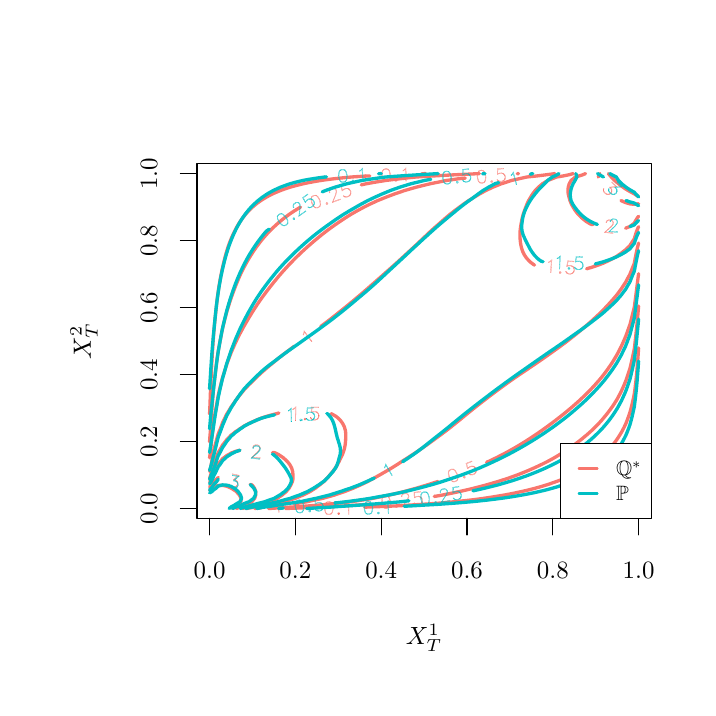
\begin{tikzpicture}[x=1pt,y=1pt]
\definecolor{fillColor}{RGB}{255,255,255}
\path[use as bounding box,fill=fillColor,fill opacity=0.00] (0,0) rectangle (238.49,238.49);
\begin{scope}
\path[clip] (  0.00,  0.00) rectangle (238.49,238.49);
\definecolor{drawColor}{RGB}{0,0,0}

\node[text=drawColor,anchor=base,inner sep=0pt, outer sep=0pt, scale=  0.90] at (143.25, 15.60) {$X^1_T$};

\node[text=drawColor,rotate= 90.00,anchor=base,inner sep=0pt, outer sep=0pt, scale=  0.90] at ( 22.80,125.25) {$X^2_T$};
\end{scope}
\begin{scope}
\path[clip] ( 61.20, 61.20) rectangle (225.29,189.29);
\definecolor{drawColor}{RGB}{248,118,109}

\path[draw=drawColor,line width= 1.2pt,line join=round,line cap=round] ( 65.73, 98.91) --
	( 65.73, 98.96) --
	( 65.78,100.19) --
	( 65.84,101.41) --
	( 65.88,102.63) --
	( 65.93,103.85) --
	( 65.98,105.08) --
	( 66.02,106.30) --
	( 66.07,107.52) --
	( 66.12,108.74) --
	( 66.18,109.97) --
	( 66.24,111.19) --
	( 66.30,112.41) --
	( 66.36,113.63) --
	( 66.41,114.85) --
	( 66.47,116.08) --
	( 66.53,117.30) --
	( 66.60,118.52) --
	( 66.67,119.74) --
	( 66.74,120.97) --
	( 66.82,122.19) --
	( 66.90,123.41) --
	( 66.98,124.63) --
	( 67.07,125.86) --
	( 67.16,127.08) --
	( 67.25,128.30) --
	( 67.29,128.80) --
	( 67.36,129.52) --
	( 67.47,130.75) --
	( 67.59,131.97) --
	( 67.71,133.19) --
	( 67.83,134.41) --
	( 67.96,135.64) --
	( 68.08,136.86) --
	( 68.22,138.08) --
	( 68.36,139.30) --
	( 68.50,140.53) --
	( 68.66,141.75) --
	( 68.83,142.97) --
	( 68.86,143.22) --
	( 69.01,144.19) --
	( 69.20,145.42) --
	( 69.41,146.64) --
	( 69.62,147.86) --
	( 69.85,149.08) --
	( 70.10,150.31) --
	( 70.36,151.53) --
	( 70.43,151.83) --
	( 70.64,152.75) --
	( 70.93,153.97) --
	( 71.24,155.20) --
	( 71.56,156.42) --
	( 71.91,157.64) --
	( 71.99,157.93) --
	( 72.29,158.86) --
	( 72.70,160.08) --
	( 73.16,161.31) --
	( 73.56,162.30) --
	( 73.66,162.53) --
	( 74.21,163.75) --
	( 74.80,164.97) --
	( 75.12,165.61) --
	( 75.44,166.20) --
	( 76.14,167.42) --
	( 76.69,168.29) --
	( 76.92,168.64) --
	( 77.79,169.86) --
	( 78.26,170.47) --
	( 78.76,171.09) --
	( 79.82,172.27) --
	( 79.86,172.31) --
	( 81.11,173.53) --
	( 81.39,173.78) --
	( 82.54,174.75) --
	( 82.95,175.07) --
	( 84.21,175.98) --
	( 84.52,176.18) --
	( 86.09,177.15) --
	( 86.16,177.20) --
	( 87.65,178.00) --
	( 88.51,178.42) --
	( 89.22,178.75) --
	( 90.78,179.41) --
	( 91.36,179.64) --
	( 92.35,180.01) --
	( 93.92,180.55) --
	( 94.92,180.87) --
	( 95.48,181.03) --
	( 97.05,181.46) --
	( 98.61,181.85) --
	( 99.63,182.09) --
	(100.18,182.21) --
	(101.75,182.53) --
	(103.31,182.82) --
	(104.88,183.10) --
	(106.18,183.31) --
	(106.44,183.35) --
	(108.01,183.56) --
	(109.58,183.76) --
	(111.14,183.94) --
	(112.71,184.11) --
	(114.27,184.27) --
	(115.84,184.42) --
	(117.03,184.53) --
	(117.41,184.56) --
	(118.97,184.66) --
	(120.54,184.76) --
	(122.10,184.86);

\path[draw=drawColor,line width= 1.2pt,line join=round,line cap=round] (142.46,185.71) --
	(143.82,185.76);

\path[draw=drawColor,line width= 1.2pt,line join=round,line cap=round] (122.10,184.86) -- (123.62,184.92);

\path[draw=drawColor,line width= 0.1pt,line join=round,line cap=round] (129.19,187.54) -- (128.52,187.29);

\path[draw=drawColor,line width= 0.1pt,line join=round,line cap=round] (128.52,187.29) -- (128.09,186.59);

\path[draw=drawColor,line width= 0.1pt,line join=round,line cap=round] (128.09,186.59) -- (127.92,185.44);

\path[draw=drawColor,line width= 0.1pt,line join=round,line cap=round] (127.92,185.44) -- (127.94,184.76);

\path[draw=drawColor,line width= 0.1pt,line join=round,line cap=round] (127.94,184.76) -- (128.22,183.64);

\path[draw=drawColor,line width= 0.1pt,line join=round,line cap=round] (128.22,183.64) -- (128.70,182.97);

\path[draw=drawColor,line width= 0.1pt,line join=round,line cap=round] (128.70,182.97) -- (129.39,182.78);

\path[draw=drawColor,line width= 0.1pt,line join=round,line cap=round] (129.39,182.78) -- (129.85,182.80);

\path[draw=drawColor,line width= 0.1pt,line join=round,line cap=round] (129.85,182.80) -- (130.52,183.05);

\path[draw=drawColor,line width= 0.1pt,line join=round,line cap=round] (130.52,183.05) -- (130.94,183.75);

\path[draw=drawColor,line width= 0.1pt,line join=round,line cap=round] (130.94,183.75) -- (131.12,184.90);

\path[draw=drawColor,line width= 0.1pt,line join=round,line cap=round] (131.12,184.90) -- (131.09,185.58);

\path[draw=drawColor,line width= 0.1pt,line join=round,line cap=round] (131.09,185.58) -- (130.82,186.70);

\path[draw=drawColor,line width= 0.1pt,line join=round,line cap=round] (130.82,186.70) -- (130.34,187.37);

\path[draw=drawColor,line width= 0.1pt,line join=round,line cap=round] (130.34,187.37) -- (129.65,187.56);

\path[draw=drawColor,line width= 0.1pt,line join=round,line cap=round] (129.65,187.56) -- (129.19,187.54);

\path[draw=drawColor,line width= 0.1pt,line join=round,line cap=round] (128.75,187.30) -- (128.32,186.60);

\path[draw=drawColor,line width= 0.1pt,line join=round,line cap=round] (128.32,186.60) -- (128.14,185.45);

\path[draw=drawColor,line width= 0.1pt,line join=round,line cap=round] (128.14,185.45) -- (128.17,184.77);

\path[draw=drawColor,line width= 0.1pt,line join=round,line cap=round] (128.17,184.77) -- (128.45,183.65);

\path[draw=drawColor,line width= 0.1pt,line join=round,line cap=round] (128.45,183.65) -- (128.93,182.98);

\path[draw=drawColor,line width= 0.1pt,line join=round,line cap=round] (128.69,183.20) -- (129.38,183.00);

\path[draw=drawColor,line width= 0.1pt,line join=round,line cap=round] (129.38,183.00) -- (129.84,183.02);

\path[draw=drawColor,line width= 0.1pt,line join=round,line cap=round] (129.84,183.02) -- (130.51,183.28);

\path[draw=drawColor,line width= 0.1pt,line join=round,line cap=round] (130.29,183.04) -- (130.72,183.74);

\path[draw=drawColor,line width= 0.1pt,line join=round,line cap=round] (130.72,183.74) -- (130.90,184.89);

\path[draw=drawColor,line width= 0.1pt,line join=round,line cap=round] (130.90,184.89) -- (130.87,185.57);

\path[draw=drawColor,line width= 0.1pt,line join=round,line cap=round] (130.87,185.57) -- (130.59,186.69);

\path[draw=drawColor,line width= 0.1pt,line join=round,line cap=round] (130.59,186.69) -- (130.11,187.36);

\path[draw=drawColor,line width= 0.1pt,line join=round,line cap=round] (130.35,187.14) -- (129.66,187.34);

\path[draw=drawColor,line width= 0.1pt,line join=round,line cap=round] (129.66,187.34) -- (129.20,187.32);

\path[draw=drawColor,line width= 0.1pt,line join=round,line cap=round] (129.20,187.32) -- (128.53,187.06);

\path[draw=drawColor,line width= 0.1pt,line join=round,line cap=round] (133.00,183.61) -- (132.78,183.37);

\path[draw=drawColor,line width= 0.1pt,line join=round,line cap=round] (132.78,183.37) -- (132.79,183.15);

\path[draw=drawColor,line width= 0.1pt,line join=round,line cap=round] (132.79,183.15) -- (133.03,182.93);

\path[draw=drawColor,line width= 0.1pt,line join=round,line cap=round] (133.03,182.93) -- (133.25,182.94);

\path[draw=drawColor,line width= 0.1pt,line join=round,line cap=round] (133.25,182.94) -- (133.47,183.17);

\path[draw=drawColor,line width= 0.1pt,line join=round,line cap=round] (133.47,183.17) -- (133.46,183.40);

\path[draw=drawColor,line width= 0.1pt,line join=round,line cap=round] (133.46,183.40) -- (133.22,183.62);

\path[draw=drawColor,line width= 0.1pt,line join=round,line cap=round] (133.22,183.62) -- (133.00,183.61);

\path[draw=drawColor,line width= 0.1pt,line join=round,line cap=round] (133.01,183.38) -- (133.02,183.16);

\path[draw=drawColor,line width= 0.1pt,line join=round,line cap=round] (133.02,183.16) -- (133.24,183.17);

\path[draw=drawColor,line width= 0.1pt,line join=round,line cap=round] (133.24,183.17) -- (133.23,183.39);

\path[draw=drawColor,line width= 0.1pt,line join=round,line cap=round] (133.23,183.39) -- (133.01,183.38);

\path[draw=drawColor,line width= 0.1pt,line join=round,line cap=round] (135.59,186.90) -- (136.03,187.15);

\path[draw=drawColor,line width= 0.1pt,line join=round,line cap=round] (136.03,187.15) -- (136.69,187.86);

\path[draw=drawColor,line width= 0.1pt,line join=round,line cap=round] (136.69,187.86) -- (136.89,183.09);

\path[draw=drawColor,line width= 0.1pt,line join=round,line cap=round] (135.59,186.90) -- (135.60,186.68);

\path[draw=drawColor,line width= 0.1pt,line join=round,line cap=round] (135.60,186.68) -- (136.04,186.92);

\path[draw=drawColor,line width= 0.1pt,line join=round,line cap=round] (136.04,186.92) -- (136.48,187.40);

\path[draw=drawColor,line width= 0.1pt,line join=round,line cap=round] (136.48,187.40) -- (136.66,183.08);

\path[draw=drawColor,line width= 0.1pt,line join=round,line cap=round] (136.66,183.08) -- (136.89,183.09);

\path[draw=drawColor,line width= 1.2pt,line join=round,line cap=round] (122.10, 65.23) --
	(123.67, 65.29) --
	(125.24, 65.35) --
	(126.80, 65.41) --
	(128.37, 65.48) --
	(129.93, 65.54) --
	(131.50, 65.61) --
	(133.07, 65.68) --
	(134.63, 65.76) --
	(136.20, 65.86) --
	(137.76, 65.96) --
	(137.76, 65.96) --
	(139.33, 66.05) --
	(140.90, 66.15) --
	(142.46, 66.24) --
	(144.03, 66.35) --
	(145.59, 66.45) --
	(147.16, 66.57) --
	(148.73, 66.69) --
	(150.29, 66.82) --
	(151.86, 66.97) --
	(153.42, 67.12) --
	(154.07, 67.18) --
	(154.99, 67.27) --
	(156.56, 67.43) --
	(158.12, 67.59) --
	(159.69, 67.76) --
	(161.25, 67.94) --
	(162.82, 68.14) --
	(164.39, 68.36) --
	(164.67, 68.40) --
	(165.95, 68.59) --
	(167.52, 68.83) --
	(169.08, 69.08) --
	(170.65, 69.34) --
	(172.22, 69.61) --
	(172.28, 69.62) --
	(173.78, 69.90) --
	(175.35, 70.20) --
	(176.91, 70.53) --
	(178.34, 70.85) --
	(178.48, 70.88) --
	(180.05, 71.23) --
	(181.61, 71.61) --
	(183.18, 72.01) --
	(183.39, 72.07) --
	(184.74, 72.44) --
	(186.31, 72.90) --
	(187.56, 73.29) --
	(187.88, 73.39) --
	(189.44, 73.92) --
	(191.01, 74.48) --
	(191.11, 74.51) --
	(192.57, 75.05) --
	(194.14, 75.68) --
	(194.29, 75.74) --
	(195.71, 76.33) --
	(197.07, 76.96) --
	(197.27, 77.05) --
	(198.84, 77.84) --
	(199.48, 78.18) --
	(200.40, 78.70) --
	(201.59, 79.40) --
	(201.97, 79.64) --
	(203.48, 80.63) --
	(203.54, 80.67) --
	(205.10, 81.77) --
	(205.21, 81.85) --
	(206.67, 82.97) --
	(206.79, 83.07) --
	(208.22, 84.29) --
	(208.23, 84.31) --
	(209.49, 85.52) --
	(209.80, 85.83) --
	(210.62, 86.74) --
	(211.37, 87.62) --
	(211.63, 87.96) --
	(212.55, 89.18) --
	(212.93, 89.72) --
	(213.39, 90.41) --
	(214.17, 91.63) --
	(214.50, 92.18) --
	(214.87, 92.85) --
	(215.51, 94.07) --
	(216.06, 95.23) --
	(216.09, 95.30) --
	(216.58, 96.52) --
	(217.03, 97.74) --
	(217.45, 98.96) --
	(217.63, 99.53) --
	(217.82,100.19) --
	(218.15,101.41) --
	(218.45,102.63) --
	(218.72,103.85) --
	(218.98,105.08) --
	(219.20,106.15) --
	(219.22,106.30) --
	(219.39,107.52) --
	(219.54,108.74) --
	(219.69,109.97) --
	(219.82,111.19) --
	(219.95,112.41) --
	(220.06,113.63) --
	(220.17,114.85) --
	(220.27,116.08) --
	(220.37,117.30) --
	(220.46,118.52) --
	(220.55,119.74) --
	(220.64,120.97) --
	(220.73,122.19) --
	(220.76,122.75);

\path[draw=drawColor,line width= 1.2pt,line join=round,line cap=round] (121.76, 65.22) -- (122.10, 65.23);

\path[draw=drawColor,line width= 0.1pt,line join=round,line cap=round] (108.52, 67.27) -- (107.85, 67.02);

\path[draw=drawColor,line width= 0.1pt,line join=round,line cap=round] (107.85, 67.02) -- (107.41, 66.33);

\path[draw=drawColor,line width= 0.1pt,line join=round,line cap=round] (107.41, 66.33) -- (107.21, 65.19);

\path[draw=drawColor,line width= 0.1pt,line join=round,line cap=round] (107.21, 65.19) -- (107.23, 64.51);

\path[draw=drawColor,line width= 0.1pt,line join=round,line cap=round] (107.23, 64.51) -- (107.49, 63.37);

\path[draw=drawColor,line width= 0.1pt,line join=round,line cap=round] (107.49, 63.37) -- (107.96, 62.70);

\path[draw=drawColor,line width= 0.1pt,line join=round,line cap=round] (107.96, 62.70) -- (108.65, 62.50);

\path[draw=drawColor,line width= 0.1pt,line join=round,line cap=round] (108.65, 62.50) -- (109.10, 62.51);

\path[draw=drawColor,line width= 0.1pt,line join=round,line cap=round] (109.10, 62.51) -- (109.78, 62.75);

\path[draw=drawColor,line width= 0.1pt,line join=round,line cap=round] (109.78, 62.75) -- (110.21, 63.44);

\path[draw=drawColor,line width= 0.1pt,line join=round,line cap=round] (110.21, 63.44) -- (110.41, 64.59);

\path[draw=drawColor,line width= 0.1pt,line join=round,line cap=round] (110.41, 64.59) -- (110.39, 65.27);

\path[draw=drawColor,line width= 0.1pt,line join=round,line cap=round] (110.39, 65.27) -- (110.14, 66.40);

\path[draw=drawColor,line width= 0.1pt,line join=round,line cap=round] (110.14, 66.40) -- (109.66, 67.07);

\path[draw=drawColor,line width= 0.1pt,line join=round,line cap=round] (109.66, 67.07) -- (108.98, 67.28);

\path[draw=drawColor,line width= 0.1pt,line join=round,line cap=round] (108.98, 67.28) -- (108.52, 67.27);

\path[draw=drawColor,line width= 0.1pt,line join=round,line cap=round] (108.07, 67.03) -- (107.64, 66.33);

\path[draw=drawColor,line width= 0.1pt,line join=round,line cap=round] (107.64, 66.33) -- (107.44, 65.19);

\path[draw=drawColor,line width= 0.1pt,line join=round,line cap=round] (107.44, 65.19) -- (107.46, 64.51);

\path[draw=drawColor,line width= 0.1pt,line join=round,line cap=round] (107.46, 64.51) -- (107.71, 63.38);

\path[draw=drawColor,line width= 0.1pt,line join=round,line cap=round] (107.71, 63.38) -- (108.19, 62.71);

\path[draw=drawColor,line width= 0.1pt,line join=round,line cap=round] (107.95, 62.93) -- (108.64, 62.72);

\path[draw=drawColor,line width= 0.1pt,line join=round,line cap=round] (108.64, 62.72) -- (109.09, 62.73);

\path[draw=drawColor,line width= 0.1pt,line join=round,line cap=round] (109.09, 62.73) -- (109.77, 62.98);

\path[draw=drawColor,line width= 0.1pt,line join=round,line cap=round] (109.55, 62.75) -- (109.99, 63.44);

\path[draw=drawColor,line width= 0.1pt,line join=round,line cap=round] (109.99, 63.44) -- (110.18, 64.58);

\path[draw=drawColor,line width= 0.1pt,line join=round,line cap=round] (110.18, 64.58) -- (110.17, 65.26);

\path[draw=drawColor,line width= 0.1pt,line join=round,line cap=round] (110.17, 65.26) -- (109.91, 66.39);

\path[draw=drawColor,line width= 0.1pt,line join=round,line cap=round] (109.91, 66.39) -- (109.44, 67.06);

\path[draw=drawColor,line width= 0.1pt,line join=round,line cap=round] (109.67, 66.84) -- (108.98, 67.05);

\path[draw=drawColor,line width= 0.1pt,line join=round,line cap=round] (108.98, 67.05) -- (108.53, 67.04);

\path[draw=drawColor,line width= 0.1pt,line join=round,line cap=round] (108.53, 67.04) -- (107.85, 66.79);

\path[draw=drawColor,line width= 0.1pt,line join=round,line cap=round] (112.26, 63.27) -- (112.04, 63.04);

\path[draw=drawColor,line width= 0.1pt,line join=round,line cap=round] (112.04, 63.04) -- (112.05, 62.81);

\path[draw=drawColor,line width= 0.1pt,line join=round,line cap=round] (112.05, 62.81) -- (112.28, 62.59);

\path[draw=drawColor,line width= 0.1pt,line join=round,line cap=round] (112.28, 62.59) -- (112.51, 62.59);

\path[draw=drawColor,line width= 0.1pt,line join=round,line cap=round] (112.51, 62.59) -- (112.73, 62.83);

\path[draw=drawColor,line width= 0.1pt,line join=round,line cap=round] (112.73, 62.83) -- (112.72, 63.05);

\path[draw=drawColor,line width= 0.1pt,line join=round,line cap=round] (112.72, 63.05) -- (112.49, 63.28);

\path[draw=drawColor,line width= 0.1pt,line join=round,line cap=round] (112.49, 63.28) -- (112.26, 63.27);

\path[draw=drawColor,line width= 0.1pt,line join=round,line cap=round] (112.27, 63.04) -- (112.27, 62.82);

\path[draw=drawColor,line width= 0.1pt,line join=round,line cap=round] (112.27, 62.82) -- (112.50, 62.82);

\path[draw=drawColor,line width= 0.1pt,line join=round,line cap=round] (112.50, 62.82) -- (112.50, 63.05);

\path[draw=drawColor,line width= 0.1pt,line join=round,line cap=round] (112.50, 63.05) -- (112.27, 63.04);

\path[draw=drawColor,line width= 0.1pt,line join=round,line cap=round] (114.91, 66.52) -- (115.36, 66.76);

\path[draw=drawColor,line width= 0.1pt,line join=round,line cap=round] (115.36, 66.76) -- (116.02, 67.46);

\path[draw=drawColor,line width= 0.1pt,line join=round,line cap=round] (116.02, 67.46) -- (116.14, 62.69);

\path[draw=drawColor,line width= 0.1pt,line join=round,line cap=round] (114.91, 66.52) -- (114.91, 66.29);

\path[draw=drawColor,line width= 0.1pt,line join=round,line cap=round] (114.91, 66.29) -- (115.36, 66.53);

\path[draw=drawColor,line width= 0.1pt,line join=round,line cap=round] (115.36, 66.53) -- (115.81, 67.00);

\path[draw=drawColor,line width= 0.1pt,line join=round,line cap=round] (115.81, 67.00) -- (115.92, 62.68);

\path[draw=drawColor,line width= 0.1pt,line join=round,line cap=round] (115.92, 62.68) -- (116.14, 62.69);

\path[draw=drawColor,line width= 1.2pt,line join=round,line cap=round] ( 65.73, 88.80) --
	( 65.75, 89.18) --
	( 65.83, 90.41) --
	( 65.93, 91.63) --
	( 66.03, 92.85) --
	( 66.11, 94.07) --
	( 66.19, 95.30) --
	( 66.26, 96.52) --
	( 66.34, 97.74) --
	( 66.43, 98.96) --
	( 66.53,100.19) --
	( 66.62,101.41) --
	( 66.72,102.63) --
	( 66.82,103.85) --
	( 66.92,105.08) --
	( 67.02,106.30) --
	( 67.12,107.52) --
	( 67.23,108.74) --
	( 67.29,109.37) --
	( 67.37,109.97) --
	( 67.51,111.19) --
	( 67.66,112.41) --
	( 67.80,113.63) --
	( 67.94,114.85) --
	( 68.09,116.08) --
	( 68.24,117.30) --
	( 68.40,118.52) --
	( 68.57,119.74) --
	( 68.76,120.97) --
	( 68.86,121.65) --
	( 68.96,122.19) --
	( 69.19,123.41) --
	( 69.41,124.63) --
	( 69.64,125.86) --
	( 69.88,127.08) --
	( 70.11,128.30) --
	( 70.36,129.52) --
	( 70.43,129.86) --
	( 70.64,130.75) --
	( 70.95,131.97) --
	( 71.26,133.19) --
	( 71.58,134.41) --
	( 71.90,135.64) --
	( 71.99,135.98) --
	( 72.26,136.86) --
	( 72.63,138.08) --
	( 73.02,139.30) --
	( 73.42,140.53) --
	( 73.56,140.94) --
	( 73.85,141.75) --
	( 74.30,142.97) --
	( 74.76,144.19) --
	( 75.12,145.16) --
	( 75.23,145.42) --
	( 75.72,146.64) --
	( 76.24,147.86) --
	( 76.69,148.91) --
	( 76.77,149.08) --
	( 77.35,150.31) --
	( 77.96,151.53) --
	( 78.26,152.11) --
	( 78.61,152.75) --
	( 79.29,153.97) --
	( 79.82,154.89) --
	( 80.01,155.20) --
	( 80.76,156.42) --
	( 81.39,157.39) --
	( 81.55,157.64) --
	( 82.39,158.86) --
	( 82.95,159.65) --
	( 83.27,160.08) --
	( 84.21,161.31) --
	( 84.52,161.69) --
	( 85.21,162.53) --
	( 86.09,163.53) --
	( 86.28,163.75) --
	( 87.43,164.97) --
	( 87.65,165.20) --
	( 88.67,166.20) --
	( 89.22,166.71) --
	( 89.99,167.42) --
	( 90.78,168.11) --
	( 91.41,168.64) --
	( 92.35,169.41) --
	( 92.93,169.86) --
	( 93.92,170.60) --
	( 94.59,171.09) --
	( 95.48,171.70) --
	( 96.41,172.31) --
	( 97.05,172.71) --
	( 98.40,173.53);

\path[draw=drawColor,line width= 1.2pt,line join=round,line cap=round] (120.54,181.68) --
	(122.10,182.03) --
	(122.38,182.09) --
	(123.67,182.32) --
	(125.24,182.60) --
	(126.80,182.86) --
	(128.37,183.11) --
	(129.62,183.31) --
	(129.93,183.35) --
	(131.50,183.54) --
	(133.07,183.72) --
	(134.63,183.90) --
	(136.20,184.08) --
	(137.76,184.26) --
	(139.33,184.42) --
	(140.41,184.53) --
	(140.90,184.56) --
	(142.46,184.66) --
	(144.03,184.76) --
	(145.59,184.85) --
	(147.16,184.94) --
	(148.73,185.03) --
	(150.29,185.12) --
	(151.86,185.20) --
	(153.42,185.28) --
	(154.99,185.36) --
	(156.56,185.43) --
	(158.12,185.50) --
	(159.69,185.58) --
	(161.25,185.66) --
	(162.82,185.73) --
	(163.21,185.76);

\path[draw=drawColor,line width= 1.2pt,line join=round,line cap=round] ( 98.40,173.53) -- ( 98.57,173.59);

\path[draw=drawColor,line width= 0.1pt,line join=round,line cap=round] (103.08,177.80) -- (102.52,177.35);

\path[draw=drawColor,line width= 0.1pt,line join=round,line cap=round] (102.52,177.35) -- (102.33,176.55);

\path[draw=drawColor,line width= 0.1pt,line join=round,line cap=round] (102.33,176.55) -- (102.51,175.41);

\path[draw=drawColor,line width= 0.1pt,line join=round,line cap=round] (102.51,175.41) -- (102.74,174.77);

\path[draw=drawColor,line width= 0.1pt,line join=round,line cap=round] (102.74,174.77) -- (103.35,173.78);

\path[draw=drawColor,line width= 0.1pt,line join=round,line cap=round] (103.35,173.78) -- (104.01,173.30);

\path[draw=drawColor,line width= 0.1pt,line join=round,line cap=round] (104.01,173.30) -- (104.73,173.32);

\path[draw=drawColor,line width= 0.1pt,line join=round,line cap=round] (104.73,173.32) -- (105.15,173.48);

\path[draw=drawColor,line width= 0.1pt,line join=round,line cap=round] (105.15,173.48) -- (105.72,173.92);

\path[draw=drawColor,line width= 0.1pt,line join=round,line cap=round] (105.72,173.92) -- (105.91,174.72);

\path[draw=drawColor,line width= 0.1pt,line join=round,line cap=round] (105.91,174.72) -- (105.73,175.87);

\path[draw=drawColor,line width= 0.1pt,line join=round,line cap=round] (105.73,175.87) -- (105.49,176.51);

\path[draw=drawColor,line width= 0.1pt,line join=round,line cap=round] (105.49,176.51) -- (104.89,177.49);

\path[draw=drawColor,line width= 0.1pt,line join=round,line cap=round] (104.89,177.49) -- (104.22,177.98);

\path[draw=drawColor,line width= 0.1pt,line join=round,line cap=round] (104.22,177.98) -- (103.50,177.95);

\path[draw=drawColor,line width= 0.1pt,line join=round,line cap=round] (103.50,177.95) -- (103.08,177.80);

\path[draw=drawColor,line width= 0.1pt,line join=round,line cap=round] (102.73,177.43) -- (102.54,176.63);

\path[draw=drawColor,line width= 0.1pt,line join=round,line cap=round] (102.54,176.63) -- (102.72,175.48);

\path[draw=drawColor,line width= 0.1pt,line join=round,line cap=round] (102.72,175.48) -- (102.95,174.84);

\path[draw=drawColor,line width= 0.1pt,line join=round,line cap=round] (102.95,174.84) -- (103.56,173.86);

\path[draw=drawColor,line width= 0.1pt,line join=round,line cap=round] (103.56,173.86) -- (104.22,173.37);

\path[draw=drawColor,line width= 0.1pt,line join=round,line cap=round] (103.93,173.51) -- (104.65,173.53);

\path[draw=drawColor,line width= 0.1pt,line join=round,line cap=round] (104.65,173.53) -- (105.08,173.69);

\path[draw=drawColor,line width= 0.1pt,line join=round,line cap=round] (105.08,173.69) -- (105.64,174.14);

\path[draw=drawColor,line width= 0.1pt,line join=round,line cap=round] (105.50,173.85) -- (105.69,174.64);

\path[draw=drawColor,line width= 0.1pt,line join=round,line cap=round] (105.69,174.64) -- (105.51,175.79);

\path[draw=drawColor,line width= 0.1pt,line join=round,line cap=round] (105.51,175.79) -- (105.28,176.43);

\path[draw=drawColor,line width= 0.1pt,line join=round,line cap=round] (105.28,176.43) -- (104.67,177.42);

\path[draw=drawColor,line width= 0.1pt,line join=round,line cap=round] (104.67,177.42) -- (104.01,177.90);

\path[draw=drawColor,line width= 0.1pt,line join=round,line cap=round] (104.30,177.76) -- (103.58,177.74);

\path[draw=drawColor,line width= 0.1pt,line join=round,line cap=round] (103.58,177.74) -- (103.16,177.58);

\path[draw=drawColor,line width= 0.1pt,line join=round,line cap=round] (103.16,177.58) -- (102.60,177.13);

\path[draw=drawColor,line width= 0.1pt,line join=round,line cap=round] (107.90,175.22) -- (107.77,174.92);

\path[draw=drawColor,line width= 0.1pt,line join=round,line cap=round] (107.77,174.92) -- (107.85,174.71);

\path[draw=drawColor,line width= 0.1pt,line join=round,line cap=round] (107.85,174.71) -- (108.14,174.58);

\path[draw=drawColor,line width= 0.1pt,line join=round,line cap=round] (108.14,174.58) -- (108.35,174.65);

\path[draw=drawColor,line width= 0.1pt,line join=round,line cap=round] (108.35,174.65) -- (108.49,174.95);

\path[draw=drawColor,line width= 0.1pt,line join=round,line cap=round] (108.49,174.95) -- (108.41,175.16);

\path[draw=drawColor,line width= 0.1pt,line join=round,line cap=round] (108.41,175.16) -- (108.12,175.29);

\path[draw=drawColor,line width= 0.1pt,line join=round,line cap=round] (108.12,175.29) -- (107.90,175.22);

\path[draw=drawColor,line width= 0.1pt,line join=round,line cap=round] (107.98,175.00) -- (108.06,174.79);

\path[draw=drawColor,line width= 0.1pt,line join=round,line cap=round] (108.06,174.79) -- (108.27,174.87);

\path[draw=drawColor,line width= 0.1pt,line join=round,line cap=round] (108.27,174.87) -- (108.20,175.08);

\path[draw=drawColor,line width= 0.1pt,line join=round,line cap=round] (108.20,175.08) -- (107.98,175.00);

\path[draw=drawColor,line width= 0.1pt,line join=round,line cap=round] (109.02,178.77) -- (108.94,178.99);

\path[draw=drawColor,line width= 0.1pt,line join=round,line cap=round] (108.94,178.99) -- (108.99,179.49);

\path[draw=drawColor,line width= 0.1pt,line join=round,line cap=round] (108.99,179.49) -- (109.13,179.78);

\path[draw=drawColor,line width= 0.1pt,line join=round,line cap=round] (109.13,179.78) -- (109.48,180.15);

\path[draw=drawColor,line width= 0.1pt,line join=round,line cap=round] (109.48,180.15) -- (110.33,180.47);

\path[draw=drawColor,line width= 0.1pt,line join=round,line cap=round] (110.33,180.47) -- (110.83,180.41);

\path[draw=drawColor,line width= 0.1pt,line join=round,line cap=round] (110.83,180.41) -- (111.13,180.28);

\path[draw=drawColor,line width= 0.1pt,line join=round,line cap=round] (111.13,180.28) -- (111.50,179.93);

\path[draw=drawColor,line width= 0.1pt,line join=round,line cap=round] (111.50,179.93) -- (111.65,179.50);

\path[draw=drawColor,line width= 0.1pt,line join=round,line cap=round] (111.65,179.50) -- (111.60,179.00);

\path[draw=drawColor,line width= 0.1pt,line join=round,line cap=round] (111.60,179.00) -- (111.41,178.20);

\path[draw=drawColor,line width= 0.1pt,line join=round,line cap=round] (111.41,178.20) -- (110.27,175.36);

\path[draw=drawColor,line width= 0.1pt,line join=round,line cap=round] (109.02,178.77) -- (109.23,178.85);

\path[draw=drawColor,line width= 0.1pt,line join=round,line cap=round] (109.23,178.85) -- (109.15,179.07);

\path[draw=drawColor,line width= 0.1pt,line join=round,line cap=round] (109.15,179.07) -- (109.21,179.57);

\path[draw=drawColor,line width= 0.1pt,line join=round,line cap=round] (109.21,179.57) -- (109.55,179.94);

\path[draw=drawColor,line width= 0.1pt,line join=round,line cap=round] (109.55,179.94) -- (110.41,180.26);

\path[draw=drawColor,line width= 0.1pt,line join=round,line cap=round] (110.41,180.26) -- (110.91,180.20);

\path[draw=drawColor,line width= 0.1pt,line join=round,line cap=round] (110.91,180.20) -- (111.28,179.85);

\path[draw=drawColor,line width= 0.1pt,line join=round,line cap=round] (111.28,179.85) -- (111.44,179.42);

\path[draw=drawColor,line width= 0.1pt,line join=round,line cap=round] (111.44,179.42) -- (111.38,178.92);

\path[draw=drawColor,line width= 0.1pt,line join=round,line cap=round] (111.38,178.92) -- (111.19,178.12);

\path[draw=drawColor,line width= 0.1pt,line join=round,line cap=round] (111.19,178.12) -- (110.06,175.28);

\path[draw=drawColor,line width= 0.1pt,line join=round,line cap=round] (110.19,175.57) -- (112.97,176.60);

\path[draw=drawColor,line width= 0.1pt,line join=round,line cap=round] (112.97,176.60) -- (113.05,176.38);

\path[draw=drawColor,line width= 0.1pt,line join=round,line cap=round] (110.06,175.28) -- (113.05,176.38);

\path[draw=drawColor,line width= 0.1pt,line join=round,line cap=round] (113.10,181.49) -- (113.60,179.49);

\path[draw=drawColor,line width= 0.1pt,line join=round,line cap=round] (113.39,181.36) -- (113.73,179.78);

\path[draw=drawColor,line width= 0.1pt,line join=round,line cap=round] (113.10,181.49) -- (115.23,182.28);

\path[draw=drawColor,line width= 0.1pt,line join=round,line cap=round] (115.23,182.28) -- (115.31,182.06);

\path[draw=drawColor,line width= 0.1pt,line join=round,line cap=round] (113.39,181.36) -- (115.31,182.06);

\path[draw=drawColor,line width= 0.1pt,line join=round,line cap=round] (113.73,179.78) -- (114.29,180.23);

\path[draw=drawColor,line width= 0.1pt,line join=round,line cap=round] (114.29,180.23) -- (114.93,180.47);

\path[draw=drawColor,line width= 0.1pt,line join=round,line cap=round] (114.93,180.47) -- (115.65,180.49);

\path[draw=drawColor,line width= 0.1pt,line join=round,line cap=round] (115.65,180.49) -- (116.23,180.22);

\path[draw=drawColor,line width= 0.1pt,line join=round,line cap=round] (116.23,180.22) -- (116.68,179.66);

\path[draw=drawColor,line width= 0.1pt,line join=round,line cap=round] (116.68,179.66) -- (116.84,179.23);

\path[draw=drawColor,line width= 0.1pt,line join=round,line cap=round] (116.84,179.23) -- (116.86,178.52);

\path[draw=drawColor,line width= 0.1pt,line join=round,line cap=round] (116.86,178.52) -- (116.59,177.93);

\path[draw=drawColor,line width= 0.1pt,line join=round,line cap=round] (116.59,177.93) -- (116.03,177.48);

\path[draw=drawColor,line width= 0.1pt,line join=round,line cap=round] (116.03,177.48) -- (115.39,177.25);

\path[draw=drawColor,line width= 0.1pt,line join=round,line cap=round] (115.39,177.25) -- (114.67,177.23);

\path[draw=drawColor,line width= 0.1pt,line join=round,line cap=round] (114.67,177.23) -- (114.38,177.36);

\path[draw=drawColor,line width= 0.1pt,line join=round,line cap=round] (114.38,177.36) -- (114.01,177.71);

\path[draw=drawColor,line width= 0.1pt,line join=round,line cap=round] (114.01,177.71) -- (114.22,177.79);

\path[draw=drawColor,line width= 0.1pt,line join=round,line cap=round] (113.60,179.49) -- (113.81,179.57);

\path[draw=drawColor,line width= 0.1pt,line join=round,line cap=round] (113.81,179.57) -- (114.16,179.94);

\path[draw=drawColor,line width= 0.1pt,line join=round,line cap=round] (114.16,179.94) -- (115.01,180.26);

\path[draw=drawColor,line width= 0.1pt,line join=round,line cap=round] (115.01,180.26) -- (115.73,180.28);

\path[draw=drawColor,line width= 0.1pt,line join=round,line cap=round] (115.73,180.28) -- (116.39,179.80);

\path[draw=drawColor,line width= 0.1pt,line join=round,line cap=round] (115.22,180.33) -- (116.02,180.14);

\path[draw=drawColor,line width= 0.1pt,line join=round,line cap=round] (116.02,180.14) -- (116.47,179.58);

\path[draw=drawColor,line width= 0.1pt,line join=round,line cap=round] (116.47,179.58) -- (116.63,179.16);

\path[draw=drawColor,line width= 0.1pt,line join=round,line cap=round] (116.63,179.16) -- (116.65,178.44);

\path[draw=drawColor,line width= 0.1pt,line join=round,line cap=round] (116.65,178.44) -- (116.17,177.78);

\path[draw=drawColor,line width= 0.1pt,line join=round,line cap=round] (116.70,178.94) -- (116.51,178.15);

\path[draw=drawColor,line width= 0.1pt,line join=round,line cap=round] (116.51,178.15) -- (115.95,177.70);

\path[draw=drawColor,line width= 0.1pt,line join=round,line cap=round] (115.95,177.70) -- (115.31,177.46);

\path[draw=drawColor,line width= 0.1pt,line join=round,line cap=round] (115.31,177.46) -- (114.59,177.44);

\path[draw=drawColor,line width= 0.1pt,line join=round,line cap=round] (114.59,177.44) -- (114.22,177.79);

\path[draw=drawColor,line width= 0.1pt,line join=round,line cap=round] (115.10,177.38) -- (114.30,177.57);

\path[draw=drawColor,line width= 1.2pt,line join=round,line cap=round] ( 93.15, 64.74) --
	( 93.92, 64.77) --
	( 95.48, 64.83) --
	( 97.05, 64.88) --
	( 98.61, 64.94) --
	(100.18, 65.01) --
	(101.75, 65.08) --
	(103.31, 65.15) --
	(104.88, 65.21) --
	(106.44, 65.27) --
	(108.01, 65.34) --
	(109.58, 65.42) --
	(111.14, 65.50) --
	(112.71, 65.59) --
	(114.27, 65.68) --
	(115.84, 65.78) --
	(117.41, 65.87) --
	(118.75, 65.96) --
	(118.97, 65.97) --
	(120.54, 66.08) --
	(122.10, 66.20) --
	(123.67, 66.33);

\path[draw=drawColor,line width= 1.2pt,line join=round,line cap=round] (147.16, 69.13) --
	(148.73, 69.40) --
	(149.96, 69.62) --
	(150.29, 69.69) --
	(151.86, 70.00) --
	(153.42, 70.32) --
	(154.99, 70.65) --
	(155.94, 70.85) --
	(156.56, 70.99) --
	(158.12, 71.34) --
	(159.69, 71.71) --
	(161.19, 72.07) --
	(161.25, 72.09) --
	(162.82, 72.49) --
	(164.39, 72.90) --
	(165.81, 73.29) --
	(165.95, 73.33) --
	(167.52, 73.78) --
	(169.08, 74.24) --
	(170.00, 74.51) --
	(170.65, 74.72) --
	(172.22, 75.22) --
	(173.77, 75.74) --
	(173.78, 75.74) --
	(175.35, 76.29) --
	(176.91, 76.87) --
	(177.14, 76.96) --
	(178.48, 77.48) --
	(180.05, 78.12) --
	(180.19, 78.18) --
	(181.61, 78.79) --
	(183.01, 79.40) --
	(183.18, 79.48) --
	(184.74, 80.20) --
	(185.63, 80.63) --
	(186.31, 80.96) --
	(187.88, 81.75) --
	(188.06, 81.85) --
	(189.44, 82.60) --
	(190.29, 83.07) --
	(191.01, 83.49) --
	(192.33, 84.29) --
	(192.57, 84.45) --
	(194.14, 85.45) --
	(194.24, 85.52) --
	(195.71, 86.50) --
	(196.05, 86.74) --
	(197.27, 87.61) --
	(197.76, 87.96) --
	(198.84, 88.77) --
	(199.38, 89.18) --
	(200.40, 89.99) --
	(200.91, 90.41) --
	(201.97, 91.29) --
	(202.36, 91.63) --
	(203.54, 92.68) --
	(203.72, 92.85) --
	(204.99, 94.07) --
	(205.10, 94.18) --
	(206.19, 95.30) --
	(206.67, 95.81) --
	(207.31, 96.52) --
	(208.23, 97.59) --
	(208.35, 97.74) --
	(209.34, 98.96) --
	(209.80, 99.55) --
	(210.28,100.19) --
	(211.17,101.41) --
	(211.37,101.68) --
	(211.99,102.63) --
	(212.76,103.85) --
	(212.93,104.13) --
	(213.45,105.08) --
	(214.10,106.30) --
	(214.50,107.09) --
	(214.69,107.52) --
	(215.24,108.74) --
	(215.76,109.97) --
	(216.06,110.70) --
	(216.24,111.19) --
	(216.67,112.41) --
	(217.08,113.63) --
	(217.47,114.85) --
	(217.63,115.35) --
	(217.81,116.08) --
	(218.10,117.30) --
	(218.37,118.52) --
	(218.64,119.74) --
	(218.90,120.97) --
	(219.15,122.19) --
	(219.20,122.41) --
	(219.32,123.41) --
	(219.46,124.63) --
	(219.60,125.86) --
	(219.73,127.08) --
	(219.86,128.30) --
	(219.99,129.52) --
	(220.11,130.75) --
	(220.23,131.97) --
	(220.35,133.19) --
	(220.46,134.41) --
	(220.56,135.64) --
	(220.67,136.86) --
	(220.76,137.92);

\path[draw=drawColor,line width= 1.2pt,line join=round,line cap=round] (146.92, 69.10) -- (147.16, 69.13);

\path[draw=drawColor,line width= 0.1pt,line join=round,line cap=round] (129.03, 69.37) -- (128.38, 69.07);

\path[draw=drawColor,line width= 0.1pt,line join=round,line cap=round] (128.38, 69.07) -- (128.01, 68.34);

\path[draw=drawColor,line width= 0.1pt,line join=round,line cap=round] (128.01, 68.34) -- (127.92, 67.18);

\path[draw=drawColor,line width= 0.1pt,line join=round,line cap=round] (127.92, 67.18) -- (128.00, 66.50);

\path[draw=drawColor,line width= 0.1pt,line join=round,line cap=round] (128.00, 66.50) -- (128.36, 65.40);

\path[draw=drawColor,line width= 0.1pt,line join=round,line cap=round] (128.36, 65.40) -- (128.89, 64.78);

\path[draw=drawColor,line width= 0.1pt,line join=round,line cap=round] (128.89, 64.78) -- (129.59, 64.63);

\path[draw=drawColor,line width= 0.1pt,line join=round,line cap=round] (129.59, 64.63) -- (130.05, 64.69);

\path[draw=drawColor,line width= 0.1pt,line join=round,line cap=round] (130.05, 64.69) -- (130.70, 65.00);

\path[draw=drawColor,line width= 0.1pt,line join=round,line cap=round] (130.70, 65.00) -- (131.07, 65.73);

\path[draw=drawColor,line width= 0.1pt,line join=round,line cap=round] (131.07, 65.73) -- (131.16, 66.88);

\path[draw=drawColor,line width= 0.1pt,line join=round,line cap=round] (131.16, 66.88) -- (131.08, 67.56);

\path[draw=drawColor,line width= 0.1pt,line join=round,line cap=round] (131.08, 67.56) -- (130.72, 68.66);

\path[draw=drawColor,line width= 0.1pt,line join=round,line cap=round] (130.72, 68.66) -- (130.19, 69.28);

\path[draw=drawColor,line width= 0.1pt,line join=round,line cap=round] (130.19, 69.28) -- (129.48, 69.43);

\path[draw=drawColor,line width= 0.1pt,line join=round,line cap=round] (129.48, 69.43) -- (129.03, 69.37);

\path[draw=drawColor,line width= 0.1pt,line join=round,line cap=round] (128.61, 69.09) -- (128.23, 68.36);

\path[draw=drawColor,line width= 0.1pt,line join=round,line cap=round] (128.23, 68.36) -- (128.14, 67.21);

\path[draw=drawColor,line width= 0.1pt,line join=round,line cap=round] (128.14, 67.21) -- (128.22, 66.53);

\path[draw=drawColor,line width= 0.1pt,line join=round,line cap=round] (128.22, 66.53) -- (128.58, 65.43);

\path[draw=drawColor,line width= 0.1pt,line join=round,line cap=round] (128.58, 65.43) -- (129.12, 64.81);

\path[draw=drawColor,line width= 0.1pt,line join=round,line cap=round] (128.86, 65.01) -- (129.57, 64.86);

\path[draw=drawColor,line width= 0.1pt,line join=round,line cap=round] (129.57, 64.86) -- (130.02, 64.91);

\path[draw=drawColor,line width= 0.1pt,line join=round,line cap=round] (130.02, 64.91) -- (130.67, 65.22);

\path[draw=drawColor,line width= 0.1pt,line join=round,line cap=round] (130.47, 64.97) -- (130.84, 65.70);

\path[draw=drawColor,line width= 0.1pt,line join=round,line cap=round] (130.84, 65.70) -- (130.93, 66.85);

\path[draw=drawColor,line width= 0.1pt,line join=round,line cap=round] (130.93, 66.85) -- (130.85, 67.53);

\path[draw=drawColor,line width= 0.1pt,line join=round,line cap=round] (130.85, 67.53) -- (130.49, 68.63);

\path[draw=drawColor,line width= 0.1pt,line join=round,line cap=round] (130.49, 68.63) -- (129.96, 69.26);

\path[draw=drawColor,line width= 0.1pt,line join=round,line cap=round] (130.21, 69.06) -- (129.51, 69.20);

\path[draw=drawColor,line width= 0.1pt,line join=round,line cap=round] (129.51, 69.20) -- (129.06, 69.15);

\path[draw=drawColor,line width= 0.1pt,line join=round,line cap=round] (129.06, 69.15) -- (128.41, 68.84);

\path[draw=drawColor,line width= 0.1pt,line join=round,line cap=round] (133.12, 65.74) -- (132.93, 65.49);

\path[draw=drawColor,line width= 0.1pt,line join=round,line cap=round] (132.93, 65.49) -- (132.95, 65.26);

\path[draw=drawColor,line width= 0.1pt,line join=round,line cap=round] (132.95, 65.26) -- (133.21, 65.07);

\path[draw=drawColor,line width= 0.1pt,line join=round,line cap=round] (133.21, 65.07) -- (133.43, 65.09);

\path[draw=drawColor,line width= 0.1pt,line join=round,line cap=round] (133.43, 65.09) -- (133.63, 65.35);

\path[draw=drawColor,line width= 0.1pt,line join=round,line cap=round] (133.63, 65.35) -- (133.60, 65.57);

\path[draw=drawColor,line width= 0.1pt,line join=round,line cap=round] (133.60, 65.57) -- (133.35, 65.77);

\path[draw=drawColor,line width= 0.1pt,line join=round,line cap=round] (133.35, 65.77) -- (133.12, 65.74);

\path[draw=drawColor,line width= 0.1pt,line join=round,line cap=round] (133.15, 65.52) -- (133.18, 65.29);

\path[draw=drawColor,line width= 0.1pt,line join=round,line cap=round] (133.18, 65.29) -- (133.40, 65.32);

\path[draw=drawColor,line width= 0.1pt,line join=round,line cap=round] (133.40, 65.32) -- (133.38, 65.54);

\path[draw=drawColor,line width= 0.1pt,line join=round,line cap=round] (133.38, 65.54) -- (133.15, 65.52);

\path[draw=drawColor,line width= 0.1pt,line join=round,line cap=round] (135.03, 68.95) -- (135.00, 69.17);

\path[draw=drawColor,line width= 0.1pt,line join=round,line cap=round] (135.00, 69.17) -- (135.18, 69.65);

\path[draw=drawColor,line width= 0.1pt,line join=round,line cap=round] (135.18, 69.65) -- (135.38, 69.90);

\path[draw=drawColor,line width= 0.1pt,line join=round,line cap=round] (135.38, 69.90) -- (135.80, 70.18);

\path[draw=drawColor,line width= 0.1pt,line join=round,line cap=round] (135.80, 70.18) -- (136.70, 70.29);

\path[draw=drawColor,line width= 0.1pt,line join=round,line cap=round] (136.70, 70.29) -- (137.18, 70.12);

\path[draw=drawColor,line width= 0.1pt,line join=round,line cap=round] (137.18, 70.12) -- (137.43, 69.92);

\path[draw=drawColor,line width= 0.1pt,line join=round,line cap=round] (137.43, 69.92) -- (137.71, 69.49);

\path[draw=drawColor,line width= 0.1pt,line join=round,line cap=round] (137.71, 69.49) -- (137.77, 69.04);

\path[draw=drawColor,line width= 0.1pt,line join=round,line cap=round] (137.77, 69.04) -- (137.60, 68.56);

\path[draw=drawColor,line width= 0.1pt,line join=round,line cap=round] (137.60, 68.56) -- (137.22, 67.83);

\path[draw=drawColor,line width= 0.1pt,line join=round,line cap=round] (137.22, 67.83) -- (135.46, 65.33);

\path[draw=drawColor,line width= 0.1pt,line join=round,line cap=round] (135.03, 68.95) -- (135.26, 68.97);

\path[draw=drawColor,line width= 0.1pt,line join=round,line cap=round] (135.26, 68.97) -- (135.23, 69.20);

\path[draw=drawColor,line width= 0.1pt,line join=round,line cap=round] (135.23, 69.20) -- (135.40, 69.68);

\path[draw=drawColor,line width= 0.1pt,line join=round,line cap=round] (135.40, 69.68) -- (135.83, 69.96);

\path[draw=drawColor,line width= 0.1pt,line join=round,line cap=round] (135.83, 69.96) -- (136.73, 70.06);

\path[draw=drawColor,line width= 0.1pt,line join=round,line cap=round] (136.73, 70.06) -- (137.21, 69.89);

\path[draw=drawColor,line width= 0.1pt,line join=round,line cap=round] (137.21, 69.89) -- (137.49, 69.47);

\path[draw=drawColor,line width= 0.1pt,line join=round,line cap=round] (137.49, 69.47) -- (137.54, 69.02);

\path[draw=drawColor,line width= 0.1pt,line join=round,line cap=round] (137.54, 69.02) -- (137.37, 68.54);

\path[draw=drawColor,line width= 0.1pt,line join=round,line cap=round] (137.37, 68.54) -- (137.00, 67.81);

\path[draw=drawColor,line width= 0.1pt,line join=round,line cap=round] (137.00, 67.81) -- (135.24, 65.31);

\path[draw=drawColor,line width= 0.1pt,line join=round,line cap=round] (135.44, 65.56) -- (138.37, 65.91);

\path[draw=drawColor,line width= 0.1pt,line join=round,line cap=round] (138.37, 65.91) -- (138.40, 65.68);

\path[draw=drawColor,line width= 0.1pt,line join=round,line cap=round] (135.24, 65.31) -- (138.40, 65.68);

\path[draw=drawColor,line width= 0.1pt,line join=round,line cap=round] (139.64, 70.64) -- (139.65, 68.58);

\path[draw=drawColor,line width= 0.1pt,line join=round,line cap=round] (139.89, 70.44) -- (139.85, 68.83);

\path[draw=drawColor,line width= 0.1pt,line join=round,line cap=round] (139.64, 70.64) -- (141.89, 70.91);

\path[draw=drawColor,line width= 0.1pt,line join=round,line cap=round] (141.89, 70.91) -- (141.92, 70.68);

\path[draw=drawColor,line width= 0.1pt,line join=round,line cap=round] (139.89, 70.44) -- (141.92, 70.68);

\path[draw=drawColor,line width= 0.1pt,line join=round,line cap=round] (139.85, 68.83) -- (140.50, 69.14);

\path[draw=drawColor,line width= 0.1pt,line join=round,line cap=round] (140.50, 69.14) -- (141.18, 69.22);

\path[draw=drawColor,line width= 0.1pt,line join=round,line cap=round] (141.18, 69.22) -- (141.88, 69.08);

\path[draw=drawColor,line width= 0.1pt,line join=round,line cap=round] (141.88, 69.08) -- (142.39, 68.68);

\path[draw=drawColor,line width= 0.1pt,line join=round,line cap=round] (142.39, 68.68) -- (142.69, 68.03);

\path[draw=drawColor,line width= 0.1pt,line join=round,line cap=round] (142.69, 68.03) -- (142.75, 67.58);

\path[draw=drawColor,line width= 0.1pt,line join=round,line cap=round] (142.75, 67.58) -- (142.60, 66.87);

\path[draw=drawColor,line width= 0.1pt,line join=round,line cap=round] (142.60, 66.87) -- (142.21, 66.37);

\path[draw=drawColor,line width= 0.1pt,line join=round,line cap=round] (142.21, 66.37) -- (141.56, 66.06);

\path[draw=drawColor,line width= 0.1pt,line join=round,line cap=round] (141.56, 66.06) -- (140.88, 65.98);

\path[draw=drawColor,line width= 0.1pt,line join=round,line cap=round] (140.88, 65.98) -- (140.17, 66.13);

\path[draw=drawColor,line width= 0.1pt,line join=round,line cap=round] (140.17, 66.13) -- (139.92, 66.32);

\path[draw=drawColor,line width= 0.1pt,line join=round,line cap=round] (139.92, 66.32) -- (139.64, 66.75);

\path[draw=drawColor,line width= 0.1pt,line join=round,line cap=round] (139.64, 66.75) -- (139.87, 66.78);

\path[draw=drawColor,line width= 0.1pt,line join=round,line cap=round] (139.65, 68.58) -- (139.88, 68.61);

\path[draw=drawColor,line width= 0.1pt,line join=round,line cap=round] (139.88, 68.61) -- (140.30, 68.89);

\path[draw=drawColor,line width= 0.1pt,line join=round,line cap=round] (140.30, 68.89) -- (141.21, 69.00);

\path[draw=drawColor,line width= 0.1pt,line join=round,line cap=round] (141.21, 69.00) -- (141.91, 68.85);

\path[draw=drawColor,line width= 0.1pt,line join=round,line cap=round] (141.91, 68.85) -- (142.44, 68.23);

\path[draw=drawColor,line width= 0.1pt,line join=round,line cap=round] (141.43, 69.02) -- (142.16, 68.65);

\path[draw=drawColor,line width= 0.1pt,line join=round,line cap=round] (142.16, 68.65) -- (142.47, 68.00);

\path[draw=drawColor,line width= 0.1pt,line join=round,line cap=round] (142.47, 68.00) -- (142.52, 67.55);

\path[draw=drawColor,line width= 0.1pt,line join=round,line cap=round] (142.52, 67.55) -- (142.38, 66.85);

\path[draw=drawColor,line width= 0.1pt,line join=round,line cap=round] (142.38, 66.85) -- (141.75, 66.31);

\path[draw=drawColor,line width= 0.1pt,line join=round,line cap=round] (142.55, 67.32) -- (142.18, 66.59);

\path[draw=drawColor,line width= 0.1pt,line join=round,line cap=round] (142.18, 66.59) -- (141.53, 66.29);

\path[draw=drawColor,line width= 0.1pt,line join=round,line cap=round] (141.53, 66.29) -- (140.85, 66.21);

\path[draw=drawColor,line width= 0.1pt,line join=round,line cap=round] (140.85, 66.21) -- (140.15, 66.35);

\path[draw=drawColor,line width= 0.1pt,line join=round,line cap=round] (140.15, 66.35) -- (139.87, 66.78);

\path[draw=drawColor,line width= 0.1pt,line join=round,line cap=round] (140.63, 66.18) -- (139.90, 66.55);

\path[draw=drawColor,line width= 1.2pt,line join=round,line cap=round] ( 65.73, 83.05) --
	( 65.73, 83.07) --
	( 65.91, 84.29) --
	( 66.07, 85.52) --
	( 66.21, 86.74) --
	( 66.33, 87.96) --
	( 66.45, 89.18) --
	( 66.58, 90.41) --
	( 66.73, 91.63) --
	( 66.87, 92.85) --
	( 67.01, 94.07) --
	( 67.15, 95.30) --
	( 67.29, 96.52) --
	( 67.29, 96.57) --
	( 67.48, 97.74) --
	( 67.69, 98.96) --
	( 67.91,100.19) --
	( 68.13,101.41) --
	( 68.35,102.63) --
	( 68.55,103.85) --
	( 68.76,105.08) --
	( 68.86,105.68) --
	( 69.00,106.30) --
	( 69.28,107.52) --
	( 69.58,108.74) --
	( 69.89,109.97) --
	( 70.20,111.19) --
	( 70.43,112.06) --
	( 70.54,112.41) --
	( 70.93,113.63) --
	( 71.31,114.85) --
	( 71.69,116.08) --
	( 71.99,117.04) --
	( 72.09,117.30) --
	( 72.54,118.52) --
	( 73.00,119.74) --
	( 73.47,120.97) --
	( 73.56,121.21) --
	( 74.00,122.19) --
	( 74.53,123.41) --
	( 75.07,124.63) --
	( 75.12,124.75) --
	( 75.67,125.86) --
	( 76.27,127.08) --
	( 76.69,127.91) --
	( 76.90,128.30) --
	( 77.56,129.52) --
	( 78.22,130.75) --
	( 78.26,130.81) --
	( 78.94,131.97) --
	( 79.65,133.19) --
	( 79.82,133.49) --
	( 80.39,134.41) --
	( 81.14,135.64) --
	( 81.39,136.04) --
	( 81.92,136.86) --
	( 82.71,138.08) --
	( 82.95,138.47) --
	( 83.53,139.30) --
	( 84.38,140.53) --
	( 84.52,140.73) --
	( 85.28,141.75) --
	( 86.09,142.85) --
	( 86.18,142.97) --
	( 87.12,144.19) --
	( 87.65,144.89) --
	( 88.07,145.42) --
	( 89.05,146.64) --
	( 89.22,146.85) --
	( 90.05,147.86) --
	( 90.78,148.74) --
	( 91.08,149.08) --
	( 92.14,150.31) --
	( 92.35,150.54) --
	( 93.25,151.53) --
	( 93.92,152.26) --
	( 94.38,152.75) --
	( 95.48,153.91) --
	( 95.55,153.97) --
	( 96.75,155.20) --
	( 97.05,155.49) --
	( 98.00,156.42) --
	( 98.61,157.00) --
	( 99.29,157.64) --
	(100.18,158.46) --
	(100.62,158.86) --
	(101.75,159.86) --
	(102.00,160.08) --
	(103.31,161.22) --
	(103.42,161.31) --
	(104.87,162.53) --
	(104.88,162.53) --
	(106.38,163.75) --
	(106.44,163.80) --
	(107.96,164.97) --
	(108.01,165.02) --
	(109.58,166.18) --
	(109.60,166.20) --
	(111.14,167.29) --
	(111.33,167.42) --
	(112.71,168.37) --
	(113.11,168.64) --
	(114.27,169.41) --
	(114.96,169.86) --
	(115.84,170.41) --
	(116.92,171.09) --
	(117.41,171.37) --
	(118.97,172.27) --
	(119.04,172.31) --
	(120.54,173.11) --
	(121.32,173.53) --
	(122.10,173.93) --
	(123.67,174.72) --
	(123.75,174.75) --
	(125.24,175.44) --
	(126.40,175.98) --
	(126.80,176.14) --
	(128.37,176.78) --
	(129.39,177.20) --
	(129.93,177.40) --
	(131.50,177.99) --
	(132.63,178.42) --
	(133.07,178.57) --
	(134.63,179.10) --
	(136.20,179.64) --
	(136.22,179.64) --
	(137.76,180.09) --
	(139.33,180.54) --
	(140.46,180.87) --
	(140.90,180.97) --
	(142.46,181.36) --
	(144.03,181.74) --
	(145.45,182.09) --
	(145.59,182.12) --
	(147.16,182.43) --
	(148.73,182.74) --
	(150.29,183.06) --
	(151.55,183.31) --
	(151.86,183.35) --
	(153.42,183.57) --
	(154.99,183.79) --
	(156.56,184.00);

\path[draw=drawColor,line width= 1.2pt,line join=round,line cap=round] (176.91,185.72) --
	(177.37,185.76);

\path[draw=drawColor,line width= 1.2pt,line join=round,line cap=round] (156.56,184.00) -- (158.12,184.13);

\path[draw=drawColor,line width= 0.1pt,line join=round,line cap=round] (163.58,186.99) -- (162.92,186.70);

\path[draw=drawColor,line width= 0.1pt,line join=round,line cap=round] (162.92,186.70) -- (162.52,185.98);

\path[draw=drawColor,line width= 0.1pt,line join=round,line cap=round] (162.52,185.98) -- (162.39,184.83);

\path[draw=drawColor,line width= 0.1pt,line join=round,line cap=round] (162.39,184.83) -- (162.45,184.15);

\path[draw=drawColor,line width= 0.1pt,line join=round,line cap=round] (162.45,184.15) -- (162.77,183.04);

\path[draw=drawColor,line width= 0.1pt,line join=round,line cap=round] (162.77,183.04) -- (163.28,182.40);

\path[draw=drawColor,line width= 0.1pt,line join=round,line cap=round] (163.28,182.40) -- (163.98,182.23);

\path[draw=drawColor,line width= 0.1pt,line join=round,line cap=round] (163.98,182.23) -- (164.43,182.27);

\path[draw=drawColor,line width= 0.1pt,line join=round,line cap=round] (164.43,182.27) -- (165.09,182.55);

\path[draw=drawColor,line width= 0.1pt,line join=round,line cap=round] (165.09,182.55) -- (165.49,183.27);

\path[draw=drawColor,line width= 0.1pt,line join=round,line cap=round] (165.49,183.27) -- (165.62,184.42);

\path[draw=drawColor,line width= 0.1pt,line join=round,line cap=round] (165.62,184.42) -- (165.56,185.10);

\path[draw=drawColor,line width= 0.1pt,line join=round,line cap=round] (165.56,185.10) -- (165.24,186.21);

\path[draw=drawColor,line width= 0.1pt,line join=round,line cap=round] (165.24,186.21) -- (164.73,186.86);

\path[draw=drawColor,line width= 0.1pt,line join=round,line cap=round] (164.73,186.86) -- (164.03,187.02);

\path[draw=drawColor,line width= 0.1pt,line join=round,line cap=round] (164.03,187.02) -- (163.58,186.99);

\path[draw=drawColor,line width= 0.1pt,line join=round,line cap=round] (163.14,186.72) -- (162.75,186.00);

\path[draw=drawColor,line width= 0.1pt,line join=round,line cap=round] (162.75,186.00) -- (162.62,184.85);

\path[draw=drawColor,line width= 0.1pt,line join=round,line cap=round] (162.62,184.85) -- (162.68,184.17);

\path[draw=drawColor,line width= 0.1pt,line join=round,line cap=round] (162.68,184.17) -- (163.00,183.06);

\path[draw=drawColor,line width= 0.1pt,line join=round,line cap=round] (163.00,183.06) -- (163.51,182.42);

\path[draw=drawColor,line width= 0.1pt,line join=round,line cap=round] (163.26,182.63) -- (163.96,182.46);

\path[draw=drawColor,line width= 0.1pt,line join=round,line cap=round] (163.96,182.46) -- (164.41,182.50);

\path[draw=drawColor,line width= 0.1pt,line join=round,line cap=round] (164.41,182.50) -- (165.07,182.78);

\path[draw=drawColor,line width= 0.1pt,line join=round,line cap=round] (164.87,182.53) -- (165.26,183.25);

\path[draw=drawColor,line width= 0.1pt,line join=round,line cap=round] (165.26,183.25) -- (165.39,184.40);

\path[draw=drawColor,line width= 0.1pt,line join=round,line cap=round] (165.39,184.40) -- (165.34,185.08);

\path[draw=drawColor,line width= 0.1pt,line join=round,line cap=round] (165.34,185.08) -- (165.01,186.20);

\path[draw=drawColor,line width= 0.1pt,line join=round,line cap=round] (165.01,186.20) -- (164.50,186.84);

\path[draw=drawColor,line width= 0.1pt,line join=round,line cap=round] (164.75,186.63) -- (164.05,186.80);

\path[draw=drawColor,line width= 0.1pt,line join=round,line cap=round] (164.05,186.80) -- (163.60,186.76);

\path[draw=drawColor,line width= 0.1pt,line join=round,line cap=round] (163.60,186.76) -- (162.94,186.48);

\path[draw=drawColor,line width= 0.1pt,line join=round,line cap=round] (167.55,183.22) -- (167.34,182.97);

\path[draw=drawColor,line width= 0.1pt,line join=round,line cap=round] (167.34,182.97) -- (167.36,182.74);

\path[draw=drawColor,line width= 0.1pt,line join=round,line cap=round] (167.36,182.74) -- (167.60,182.54);

\path[draw=drawColor,line width= 0.1pt,line join=round,line cap=round] (167.60,182.54) -- (167.83,182.56);

\path[draw=drawColor,line width= 0.1pt,line join=round,line cap=round] (167.83,182.56) -- (168.04,182.80);

\path[draw=drawColor,line width= 0.1pt,line join=round,line cap=round] (168.04,182.80) -- (168.02,183.03);

\path[draw=drawColor,line width= 0.1pt,line join=round,line cap=round] (168.02,183.03) -- (167.77,183.24);

\path[draw=drawColor,line width= 0.1pt,line join=round,line cap=round] (167.77,183.24) -- (167.55,183.22);

\path[draw=drawColor,line width= 0.1pt,line join=round,line cap=round] (167.57,182.99) -- (167.59,182.76);

\path[draw=drawColor,line width= 0.1pt,line join=round,line cap=round] (167.59,182.76) -- (167.81,182.78);

\path[draw=drawColor,line width= 0.1pt,line join=round,line cap=round] (167.81,182.78) -- (167.79,183.01);

\path[draw=drawColor,line width= 0.1pt,line join=round,line cap=round] (167.79,183.01) -- (167.57,182.99);

\path[draw=drawColor,line width= 0.1pt,line join=round,line cap=round] (169.69,187.50) -- (169.64,185.45);

\path[draw=drawColor,line width= 0.1pt,line join=round,line cap=round] (169.94,187.30) -- (169.85,185.69);

\path[draw=drawColor,line width= 0.1pt,line join=round,line cap=round] (169.69,187.50) -- (171.96,187.70);

\path[draw=drawColor,line width= 0.1pt,line join=round,line cap=round] (171.96,187.70) -- (171.98,187.47);

\path[draw=drawColor,line width= 0.1pt,line join=round,line cap=round] (169.94,187.30) -- (171.98,187.47);

\path[draw=drawColor,line width= 0.1pt,line join=round,line cap=round] (169.85,185.69) -- (170.51,185.98);

\path[draw=drawColor,line width= 0.1pt,line join=round,line cap=round] (170.51,185.98) -- (171.19,186.03);

\path[draw=drawColor,line width= 0.1pt,line join=round,line cap=round] (171.19,186.03) -- (171.88,185.86);

\path[draw=drawColor,line width= 0.1pt,line join=round,line cap=round] (171.88,185.86) -- (172.38,185.45);

\path[draw=drawColor,line width= 0.1pt,line join=round,line cap=round] (172.38,185.45) -- (172.66,184.79);

\path[draw=drawColor,line width= 0.1pt,line join=round,line cap=round] (172.66,184.79) -- (172.70,184.34);

\path[draw=drawColor,line width= 0.1pt,line join=round,line cap=round] (172.70,184.34) -- (172.53,183.64);

\path[draw=drawColor,line width= 0.1pt,line join=round,line cap=round] (172.53,183.64) -- (172.11,183.15);

\path[draw=drawColor,line width= 0.1pt,line join=round,line cap=round] (172.11,183.15) -- (171.45,182.86);

\path[draw=drawColor,line width= 0.1pt,line join=round,line cap=round] (171.45,182.86) -- (170.77,182.81);

\path[draw=drawColor,line width= 0.1pt,line join=round,line cap=round] (170.77,182.81) -- (170.08,182.97);

\path[draw=drawColor,line width= 0.1pt,line join=round,line cap=round] (170.08,182.97) -- (169.83,183.18);

\path[draw=drawColor,line width= 0.1pt,line join=round,line cap=round] (169.83,183.18) -- (169.57,183.62);

\path[draw=drawColor,line width= 0.1pt,line join=round,line cap=round] (169.57,183.62) -- (169.79,183.63);

\path[draw=drawColor,line width= 0.1pt,line join=round,line cap=round] (169.64,185.45) -- (169.87,185.47);

\path[draw=drawColor,line width= 0.1pt,line join=round,line cap=round] (169.87,185.47) -- (170.30,185.73);

\path[draw=drawColor,line width= 0.1pt,line join=round,line cap=round] (170.30,185.73) -- (171.20,185.81);

\path[draw=drawColor,line width= 0.1pt,line join=round,line cap=round] (171.20,185.81) -- (171.90,185.64);

\path[draw=drawColor,line width= 0.1pt,line join=round,line cap=round] (171.90,185.64) -- (172.41,185.00);

\path[draw=drawColor,line width= 0.1pt,line join=round,line cap=round] (171.43,185.83) -- (172.15,185.43);

\path[draw=drawColor,line width= 0.1pt,line join=round,line cap=round] (172.15,185.43) -- (172.43,184.77);

\path[draw=drawColor,line width= 0.1pt,line join=round,line cap=round] (172.43,184.77) -- (172.47,184.32);

\path[draw=drawColor,line width= 0.1pt,line join=round,line cap=round] (172.47,184.32) -- (172.30,183.62);

\path[draw=drawColor,line width= 0.1pt,line join=round,line cap=round] (172.30,183.62) -- (171.66,183.11);

\path[draw=drawColor,line width= 0.1pt,line join=round,line cap=round] (172.49,184.09) -- (172.10,183.37);

\path[draw=drawColor,line width= 0.1pt,line join=round,line cap=round] (172.10,183.37) -- (171.44,183.09);

\path[draw=drawColor,line width= 0.1pt,line join=round,line cap=round] (171.44,183.09) -- (170.76,183.03);

\path[draw=drawColor,line width= 0.1pt,line join=round,line cap=round] (170.76,183.03) -- (170.06,183.20);

\path[draw=drawColor,line width= 0.1pt,line join=round,line cap=round] (170.06,183.20) -- (169.79,183.63);

\path[draw=drawColor,line width= 0.1pt,line join=round,line cap=round] (170.53,183.01) -- (169.81,183.41);

\path[draw=drawColor,line width= 1.2pt,line join=round,line cap=round] ( 87.05, 64.74) --
	( 87.65, 64.77) --
	( 89.22, 64.86) --
	( 90.78, 64.98) --
	( 92.35, 65.10) --
	( 93.92, 65.19) --
	( 95.48, 65.28) --
	( 97.05, 65.37) --
	( 98.61, 65.47) --
	(100.18, 65.59) --
	(101.75, 65.70) --
	(103.31, 65.82) --
	(104.88, 65.93) --
	(105.21, 65.96) --
	(106.44, 66.08) --
	(108.01, 66.23) --
	(109.58, 66.39) --
	(111.14, 66.57) --
	(112.71, 66.74) --
	(114.27, 66.92) --
	(115.84, 67.09) --
	(116.67, 67.18) --
	(117.41, 67.29) --
	(118.97, 67.51) --
	(120.54, 67.74) --
	(122.10, 67.98) --
	(123.67, 68.23) --
	(124.70, 68.40) --
	(125.24, 68.51) --
	(126.80, 68.83) --
	(128.37, 69.14) --
	(129.93, 69.45) --
	(130.79, 69.62) --
	(131.50, 69.79) --
	(133.07, 70.15) --
	(134.63, 70.52) --
	(135.99, 70.85) --
	(136.20, 70.91) --
	(137.76, 71.34) --
	(139.33, 71.78) --
	(140.39, 72.07) --
	(140.90, 72.22) --
	(142.46, 72.69) --
	(144.03, 73.16) --
	(144.46, 73.29) --
	(145.59, 73.66) --
	(147.16, 74.16) --
	(148.24, 74.51);

\path[draw=drawColor,line width= 1.2pt,line join=round,line cap=round] (165.95, 81.47) --
	(166.77, 81.85) --
	(167.52, 82.21) --
	(169.08, 82.97) --
	(169.30, 83.07) --
	(170.65, 83.76) --
	(171.70, 84.29) --
	(172.22, 84.57) --
	(173.78, 85.41) --
	(173.97, 85.52) --
	(175.35, 86.29) --
	(176.13, 86.74) --
	(176.91, 87.20) --
	(178.19, 87.96) --
	(178.48, 88.14) --
	(180.05, 89.11) --
	(180.16, 89.18) --
	(181.61, 90.12) --
	(182.06, 90.41) --
	(183.18, 91.15) --
	(183.88, 91.63) --
	(184.74, 92.22) --
	(185.65, 92.85) --
	(186.31, 93.32) --
	(187.36, 94.07) --
	(187.88, 94.45) --
	(189.02, 95.30) --
	(189.44, 95.61) --
	(190.65, 96.52) --
	(191.01, 96.80) --
	(192.23, 97.74) --
	(192.57, 98.01) --
	(193.77, 98.96) --
	(194.14, 99.27) --
	(195.26,100.19) --
	(195.71,100.56) --
	(196.70,101.41) --
	(197.27,101.90) --
	(198.10,102.63) --
	(198.84,103.28) --
	(199.46,103.85) --
	(200.40,104.73) --
	(200.77,105.08) --
	(201.97,106.24) --
	(202.03,106.30) --
	(203.23,107.52) --
	(203.54,107.84) --
	(204.38,108.74) --
	(205.10,109.52) --
	(205.49,109.97) --
	(206.57,111.19) --
	(206.67,111.30) --
	(207.58,112.41) --
	(208.23,113.22) --
	(208.54,113.63) --
	(209.43,114.85) --
	(209.80,115.36) --
	(210.29,116.08) --
	(211.11,117.30) --
	(211.37,117.69) --
	(211.87,118.52) --
	(212.61,119.74) --
	(212.93,120.29) --
	(213.29,120.97) --
	(213.92,122.19) --
	(214.50,123.32) --
	(214.54,123.41) --
	(215.09,124.63) --
	(215.63,125.86) --
	(216.06,126.84) --
	(216.15,127.08) --
	(216.59,128.30) --
	(217.02,129.52) --
	(217.46,130.75) --
	(217.63,131.21) --
	(217.83,131.97) --
	(218.14,133.19) --
	(218.44,134.41) --
	(218.74,135.64) --
	(219.05,136.86) --
	(219.20,137.45) --
	(219.28,138.08) --
	(219.44,139.30) --
	(219.60,140.53) --
	(219.76,141.75) --
	(219.92,142.97) --
	(220.07,144.19) --
	(220.22,145.42) --
	(220.37,146.64) --
	(220.53,147.86) --
	(220.69,149.08) --
	(220.76,149.59);

\path[draw=drawColor,line width= 1.2pt,line join=round,line cap=round] (165.80, 81.41) -- (165.95, 81.47);

\path[draw=drawColor,line width= 0.1pt,line join=round,line cap=round] (152.66, 78.81) -- (152.10, 78.35);

\path[draw=drawColor,line width= 0.1pt,line join=round,line cap=round] (152.10, 78.35) -- (151.93, 77.55);

\path[draw=drawColor,line width= 0.1pt,line join=round,line cap=round] (151.93, 77.55) -- (152.13, 76.41);

\path[draw=drawColor,line width= 0.1pt,line join=round,line cap=round] (152.13, 76.41) -- (152.38, 75.78);

\path[draw=drawColor,line width= 0.1pt,line join=round,line cap=round] (152.38, 75.78) -- (153.01, 74.80);

\path[draw=drawColor,line width= 0.1pt,line join=round,line cap=round] (153.01, 74.80) -- (153.68, 74.33);

\path[draw=drawColor,line width= 0.1pt,line join=round,line cap=round] (153.68, 74.33) -- (154.40, 74.37);

\path[draw=drawColor,line width= 0.1pt,line join=round,line cap=round] (154.40, 74.37) -- (154.82, 74.54);

\path[draw=drawColor,line width= 0.1pt,line join=round,line cap=round] (154.82, 74.54) -- (155.38, 75.00);

\path[draw=drawColor,line width= 0.1pt,line join=round,line cap=round] (155.38, 75.00) -- (155.55, 75.80);

\path[draw=drawColor,line width= 0.1pt,line join=round,line cap=round] (155.55, 75.80) -- (155.35, 76.94);

\path[draw=drawColor,line width= 0.1pt,line join=round,line cap=round] (155.35, 76.94) -- (155.10, 77.57);

\path[draw=drawColor,line width= 0.1pt,line join=round,line cap=round] (155.10, 77.57) -- (154.47, 78.55);

\path[draw=drawColor,line width= 0.1pt,line join=round,line cap=round] (154.47, 78.55) -- (153.80, 79.02);

\path[draw=drawColor,line width= 0.1pt,line join=round,line cap=round] (153.80, 79.02) -- (153.08, 78.98);

\path[draw=drawColor,line width= 0.1pt,line join=round,line cap=round] (153.08, 78.98) -- (152.66, 78.81);

\path[draw=drawColor,line width= 0.1pt,line join=round,line cap=round] (152.32, 78.44) -- (152.14, 77.63);

\path[draw=drawColor,line width= 0.1pt,line join=round,line cap=round] (152.14, 77.63) -- (152.35, 76.49);

\path[draw=drawColor,line width= 0.1pt,line join=round,line cap=round] (152.35, 76.49) -- (152.60, 75.86);

\path[draw=drawColor,line width= 0.1pt,line join=round,line cap=round] (152.60, 75.86) -- (153.22, 74.88);

\path[draw=drawColor,line width= 0.1pt,line join=round,line cap=round] (153.22, 74.88) -- (153.89, 74.42);

\path[draw=drawColor,line width= 0.1pt,line join=round,line cap=round] (153.60, 74.54) -- (154.32, 74.58);

\path[draw=drawColor,line width= 0.1pt,line join=round,line cap=round] (154.32, 74.58) -- (154.74, 74.75);

\path[draw=drawColor,line width= 0.1pt,line join=round,line cap=round] (154.74, 74.75) -- (155.29, 75.21);

\path[draw=drawColor,line width= 0.1pt,line join=round,line cap=round] (155.16, 74.91) -- (155.34, 75.72);

\path[draw=drawColor,line width= 0.1pt,line join=round,line cap=round] (155.34, 75.72) -- (155.13, 76.86);

\path[draw=drawColor,line width= 0.1pt,line join=round,line cap=round] (155.13, 76.86) -- (154.88, 77.49);

\path[draw=drawColor,line width= 0.1pt,line join=round,line cap=round] (154.88, 77.49) -- (154.26, 78.47);

\path[draw=drawColor,line width= 0.1pt,line join=round,line cap=round] (154.26, 78.47) -- (153.58, 78.93);

\path[draw=drawColor,line width= 0.1pt,line join=round,line cap=round] (153.88, 78.81) -- (153.16, 78.77);

\path[draw=drawColor,line width= 0.1pt,line join=round,line cap=round] (153.16, 78.77) -- (152.74, 78.60);

\path[draw=drawColor,line width= 0.1pt,line join=round,line cap=round] (152.74, 78.60) -- (152.19, 78.14);

\path[draw=drawColor,line width= 0.1pt,line join=round,line cap=round] (157.54, 76.34) -- (157.41, 76.04);

\path[draw=drawColor,line width= 0.1pt,line join=round,line cap=round] (157.41, 76.04) -- (157.49, 75.83);

\path[draw=drawColor,line width= 0.1pt,line join=round,line cap=round] (157.49, 75.83) -- (157.79, 75.70);

\path[draw=drawColor,line width= 0.1pt,line join=round,line cap=round] (157.79, 75.70) -- (158.00, 75.78);

\path[draw=drawColor,line width= 0.1pt,line join=round,line cap=round] (158.00, 75.78) -- (158.13, 76.08);

\path[draw=drawColor,line width= 0.1pt,line join=round,line cap=round] (158.13, 76.08) -- (158.04, 76.29);

\path[draw=drawColor,line width= 0.1pt,line join=round,line cap=round] (158.04, 76.29) -- (157.75, 76.42);

\path[draw=drawColor,line width= 0.1pt,line join=round,line cap=round] (157.75, 76.42) -- (157.54, 76.34);

\path[draw=drawColor,line width= 0.1pt,line join=round,line cap=round] (157.62, 76.12) -- (157.70, 75.91);

\path[draw=drawColor,line width= 0.1pt,line join=round,line cap=round] (157.70, 75.91) -- (157.91, 76.00);

\path[draw=drawColor,line width= 0.1pt,line join=round,line cap=round] (157.91, 76.00) -- (157.83, 76.21);

\path[draw=drawColor,line width= 0.1pt,line join=round,line cap=round] (157.83, 76.21) -- (157.62, 76.12);

\path[draw=drawColor,line width= 0.1pt,line join=round,line cap=round] (158.37, 81.06) -- (158.90, 79.07);

\path[draw=drawColor,line width= 0.1pt,line join=round,line cap=round] (158.66, 80.93) -- (159.03, 79.36);

\path[draw=drawColor,line width= 0.1pt,line join=round,line cap=round] (158.37, 81.06) -- (160.48, 81.89);

\path[draw=drawColor,line width= 0.1pt,line join=round,line cap=round] (160.48, 81.89) -- (160.57, 81.68);

\path[draw=drawColor,line width= 0.1pt,line join=round,line cap=round] (158.66, 80.93) -- (160.57, 81.68);

\path[draw=drawColor,line width= 0.1pt,line join=round,line cap=round] (159.03, 79.36) -- (159.58, 79.83);

\path[draw=drawColor,line width= 0.1pt,line join=round,line cap=round] (159.58, 79.83) -- (160.22, 80.07);

\path[draw=drawColor,line width= 0.1pt,line join=round,line cap=round] (160.22, 80.07) -- (160.94, 80.11);

\path[draw=drawColor,line width= 0.1pt,line join=round,line cap=round] (160.94, 80.11) -- (161.52, 79.86);

\path[draw=drawColor,line width= 0.1pt,line join=round,line cap=round] (161.52, 79.86) -- (161.99, 79.30);

\path[draw=drawColor,line width= 0.1pt,line join=round,line cap=round] (161.99, 79.30) -- (162.15, 78.88);

\path[draw=drawColor,line width= 0.1pt,line join=round,line cap=round] (162.15, 78.88) -- (162.19, 78.16);

\path[draw=drawColor,line width= 0.1pt,line join=round,line cap=round] (162.19, 78.16) -- (161.93, 77.57);

\path[draw=drawColor,line width= 0.1pt,line join=round,line cap=round] (161.93, 77.57) -- (161.38, 77.11);

\path[draw=drawColor,line width= 0.1pt,line join=round,line cap=round] (161.38, 77.11) -- (160.75, 76.86);

\path[draw=drawColor,line width= 0.1pt,line join=round,line cap=round] (160.75, 76.86) -- (160.03, 76.83);

\path[draw=drawColor,line width= 0.1pt,line join=round,line cap=round] (160.03, 76.83) -- (159.73, 76.95);

\path[draw=drawColor,line width= 0.1pt,line join=round,line cap=round] (159.73, 76.95) -- (159.36, 77.29);

\path[draw=drawColor,line width= 0.1pt,line join=round,line cap=round] (159.36, 77.29) -- (159.57, 77.38);

\path[draw=drawColor,line width= 0.1pt,line join=round,line cap=round] (158.90, 79.07) -- (159.11, 79.15);

\path[draw=drawColor,line width= 0.1pt,line join=round,line cap=round] (159.11, 79.15) -- (159.45, 79.53);

\path[draw=drawColor,line width= 0.1pt,line join=round,line cap=round] (159.45, 79.53) -- (160.30, 79.86);

\path[draw=drawColor,line width= 0.1pt,line join=round,line cap=round] (160.30, 79.86) -- (161.02, 79.90);

\path[draw=drawColor,line width= 0.1pt,line join=round,line cap=round] (161.02, 79.90) -- (161.69, 79.43);

\path[draw=drawColor,line width= 0.1pt,line join=round,line cap=round] (160.51, 79.95) -- (161.31, 79.77);

\path[draw=drawColor,line width= 0.1pt,line join=round,line cap=round] (161.31, 79.77) -- (161.77, 79.22);

\path[draw=drawColor,line width= 0.1pt,line join=round,line cap=round] (161.77, 79.22) -- (161.94, 78.80);

\path[draw=drawColor,line width= 0.1pt,line join=round,line cap=round] (161.94, 78.80) -- (161.98, 78.08);

\path[draw=drawColor,line width= 0.1pt,line join=round,line cap=round] (161.98, 78.08) -- (161.51, 77.41);

\path[draw=drawColor,line width= 0.1pt,line join=round,line cap=round] (162.02, 78.59) -- (161.85, 77.79);

\path[draw=drawColor,line width= 0.1pt,line join=round,line cap=round] (161.85, 77.79) -- (161.30, 77.32);

\path[draw=drawColor,line width= 0.1pt,line join=round,line cap=round] (161.30, 77.32) -- (160.66, 77.08);

\path[draw=drawColor,line width= 0.1pt,line join=round,line cap=round] (160.66, 77.08) -- (159.95, 77.04);

\path[draw=drawColor,line width= 0.1pt,line join=round,line cap=round] (159.95, 77.04) -- (159.57, 77.38);

\path[draw=drawColor,line width= 0.1pt,line join=round,line cap=round] (160.45, 76.99) -- (159.65, 77.17);

\path[draw=drawColor,line width= 1.2pt,line join=round,line cap=round] ( 65.73, 78.12) --
	( 65.75, 78.18) --
	( 66.07, 79.40) --
	( 66.32, 80.63) --
	( 66.53, 81.85) --
	( 66.74, 83.07) --
	( 66.98, 84.29) --
	( 67.21, 85.52) --
	( 67.29, 85.99) --
	( 67.51, 86.74) --
	( 67.84, 87.96) --
	( 68.15, 89.18) --
	( 68.48, 90.41) --
	( 68.84, 91.63) --
	( 68.86, 91.72) --
	( 69.34, 92.85) --
	( 69.82, 94.07) --
	( 70.27, 95.30) --
	( 70.43, 95.75) --
	( 70.81, 96.52) --
	( 71.40, 97.74) --
	( 71.99, 98.93) --
	( 72.01, 98.96) --
	( 72.78,100.19) --
	( 73.51,101.41) --
	( 73.56,101.50) --
	( 74.37,102.63) --
	( 75.12,103.75) --
	( 75.21,103.85) --
	( 76.16,105.08) --
	( 76.69,105.79) --
	( 77.12,106.30) --
	( 78.12,107.52) --
	( 78.26,107.69) --
	( 79.26,108.74) --
	( 79.82,109.35) --
	( 80.46,109.97) --
	( 81.39,110.89) --
	( 81.70,111.19) --
	( 82.95,112.41) --
	( 82.95,112.42) --
	( 84.26,113.63) --
	( 84.52,113.88) --
	( 85.64,114.85) --
	( 86.09,115.26) --
	( 87.07,116.08) --
	( 87.65,116.58) --
	( 88.54,117.30) --
	( 89.22,117.87) --
	( 90.03,118.52) --
	( 90.78,119.15) --
	( 91.55,119.74) --
	( 92.35,120.38) --
	( 93.13,120.97) --
	( 93.92,121.58) --
	( 94.74,122.19) --
	( 95.48,122.75) --
	( 96.38,123.41);

\path[draw=drawColor,line width= 1.2pt,line join=round,line cap=round] (106.22,130.75) --
	(106.44,130.92) --
	(107.84,131.97) --
	(108.01,132.10) --
	(109.43,133.19) --
	(109.58,133.31) --
	(110.99,134.41) --
	(111.14,134.54) --
	(112.52,135.64) --
	(112.71,135.79) --
	(114.05,136.86) --
	(114.27,137.04) --
	(115.55,138.08) --
	(115.84,138.32) --
	(117.03,139.30) --
	(117.41,139.61) --
	(118.50,140.53) --
	(118.97,140.92) --
	(119.95,141.75) --
	(120.54,142.25) --
	(121.38,142.97) --
	(122.10,143.60) --
	(122.79,144.19) --
	(123.67,144.96) --
	(124.19,145.42) --
	(125.24,146.33) --
	(125.59,146.64) --
	(126.80,147.71) --
	(126.98,147.86) --
	(128.36,149.08) --
	(128.37,149.09) --
	(129.75,150.31) --
	(129.93,150.47) --
	(131.13,151.53) --
	(131.50,151.86) --
	(132.50,152.75) --
	(133.07,153.26) --
	(133.85,153.97) --
	(134.63,154.68) --
	(135.20,155.20) --
	(136.20,156.11) --
	(136.53,156.42) --
	(137.76,157.56) --
	(137.85,157.64) --
	(139.18,158.86) --
	(139.33,159.00) --
	(140.50,160.08) --
	(140.90,160.46) --
	(141.79,161.31) --
	(142.46,161.94) --
	(143.07,162.53) --
	(144.03,163.43) --
	(144.36,163.75) --
	(145.59,164.91) --
	(145.67,164.97) --
	(147.02,166.20) --
	(147.16,166.32) --
	(148.42,167.42) --
	(148.73,167.69) --
	(149.80,168.64) --
	(150.29,169.06) --
	(151.20,169.86) --
	(151.86,170.41) --
	(152.66,171.09) --
	(153.42,171.67) --
	(154.23,172.31) --
	(154.99,172.87) --
	(155.87,173.53) --
	(156.56,174.03) --
	(157.53,174.75) --
	(158.12,175.15) --
	(159.31,175.98) --
	(159.69,176.20) --
	(161.25,177.17) --
	(161.29,177.20) --
	(162.82,178.11) --
	(163.31,178.42) --
	(164.39,179.00) --
	(165.52,179.64) --
	(165.95,179.84) --
	(167.52,180.57) --
	(168.13,180.87) --
	(169.08,181.24) --
	(170.65,181.88) --
	(171.14,182.09) --
	(172.22,182.41) --
	(173.78,182.92) --
	(174.92,183.31) --
	(175.35,183.40) --
	(176.91,183.75) --
	(178.48,184.10) --
	(180.05,184.46) --
	(180.36,184.53) --
	(181.61,184.66) --
	(183.18,184.82) --
	(184.74,185.00) --
	(186.31,185.19) --
	(187.88,185.40) --
	(189.44,185.60) --
	(190.53,185.76);

\path[draw=drawColor,line width= 1.2pt,line join=round,line cap=round] (105.86,130.47) -- (106.22,130.75);

\path[draw=drawColor,line width= 0.1pt,line join=round,line cap=round] ( 99.51,127.59) -- ( 99.73,128.04);

\path[draw=drawColor,line width= 0.1pt,line join=round,line cap=round] ( 99.73,128.04) -- ( 99.87,128.99);

\path[draw=drawColor,line width= 0.1pt,line join=round,line cap=round] ( 99.87,128.99) -- (102.73,125.17);

\path[draw=drawColor,line width= 0.1pt,line join=round,line cap=round] ( 99.51,127.59) -- ( 99.64,127.40);

\path[draw=drawColor,line width= 0.1pt,line join=round,line cap=round] ( 99.64,127.40) -- ( 99.87,127.86);

\path[draw=drawColor,line width= 0.1pt,line join=round,line cap=round] ( 99.87,127.86) -- ( 99.96,128.49);

\path[draw=drawColor,line width= 0.1pt,line join=round,line cap=round] ( 99.96,128.49) -- (102.54,125.03);

\path[draw=drawColor,line width= 0.1pt,line join=round,line cap=round] (102.54,125.03) -- (102.73,125.17);

\path[draw=drawColor,line width= 1.2pt,line join=round,line cap=round] ( 82.02, 64.74) --
	( 82.95, 64.87) --
	( 84.52, 65.09);

\path[draw=drawColor,line width= 1.2pt,line join=round,line cap=round] ( 97.05, 66.56) --
	( 98.61, 66.80) --
	(100.18, 67.06) --
	(100.94, 67.18) --
	(101.75, 67.37) --
	(103.31, 67.72) --
	(104.88, 68.05) --
	(106.44, 68.37) --
	(106.60, 68.40) --
	(108.01, 68.80) --
	(109.58, 69.24) --
	(110.92, 69.62) --
	(111.14, 69.71) --
	(112.71, 70.25) --
	(114.27, 70.77) --
	(114.52, 70.85) --
	(115.84, 71.38) --
	(117.41, 71.99) --
	(117.61, 72.07) --
	(118.97, 72.68) --
	(120.38, 73.29) --
	(120.54, 73.37) --
	(122.10, 74.13) --
	(122.93, 74.51) --
	(123.67, 74.93) --
	(125.20, 75.74) --
	(125.24, 75.76) --
	(126.80, 76.65) --
	(127.38, 76.96) --
	(128.37, 77.54) --
	(129.52, 78.18) --
	(129.93, 78.44) --
	(131.50, 79.36) --
	(131.57, 79.40) --
	(133.07, 80.35) --
	(133.53, 80.63) --
	(134.63, 81.35) --
	(135.43, 81.85) --
	(136.20, 82.36) --
	(137.33, 83.07) --
	(137.76, 83.36) --
	(139.22, 84.29) --
	(139.33, 84.37) --
	(140.90, 85.41) --
	(141.06, 85.52) --
	(142.46, 86.49) --
	(142.83, 86.74) --
	(144.03, 87.59) --
	(144.56, 87.96) --
	(145.59, 88.72) --
	(146.25, 89.18) --
	(147.16, 89.86) --
	(147.92, 90.41) --
	(148.73, 91.00) --
	(149.59, 91.63) --
	(150.29, 92.17) --
	(151.21, 92.85) --
	(151.86, 93.36) --
	(152.79, 94.07) --
	(153.42, 94.59) --
	(154.32, 95.30) --
	(154.99, 95.84) --
	(155.83, 96.52) --
	(156.56, 97.12) --
	(157.31, 97.74) --
	(158.12, 98.41) --
	(158.81, 98.96) --
	(159.69, 99.68) --
	(160.33,100.19) --
	(161.25,100.94) --
	(161.85,101.41) --
	(162.82,102.18) --
	(163.40,102.63) --
	(164.39,103.40) --
	(164.97,103.85) --
	(165.95,104.61) --
	(166.57,105.08) --
	(167.52,105.79) --
	(168.19,106.30) --
	(169.08,106.97) --
	(169.82,107.52) --
	(170.65,108.13) --
	(171.48,108.74) --
	(172.22,109.28) --
	(173.17,109.97) --
	(173.78,110.40) --
	(174.89,111.19) --
	(175.35,111.51) --
	(176.65,112.41) --
	(176.91,112.59) --
	(178.44,113.63) --
	(178.48,113.66) --
	(180.05,114.71) --
	(180.26,114.85) --
	(181.61,115.76) --
	(182.08,116.08) --
	(183.18,116.82) --
	(183.88,117.30) --
	(184.74,117.89) --
	(185.65,118.52) --
	(186.31,118.98) --
	(187.39,119.74) --
	(187.88,120.08) --
	(189.12,120.97) --
	(189.44,121.20) --
	(190.83,122.19) --
	(191.01,122.31) --
	(192.53,123.41) --
	(192.57,123.44) --
	(194.14,124.60) --
	(194.19,124.63) --
	(195.71,125.80) --
	(195.78,125.86) --
	(197.27,127.04) --
	(197.32,127.08) --
	(198.84,128.30) --
	(198.84,128.30) --
	(200.33,129.52) --
	(200.40,129.58) --
	(201.78,130.75) --
	(201.97,130.90) --
	(203.17,131.97) --
	(203.54,132.28) --
	(204.52,133.19) --
	(205.10,133.72) --
	(205.84,134.41) --
	(206.67,135.17) --
	(207.12,135.64) --
	(208.23,136.73) --
	(208.35,136.86) --
	(209.48,138.08) --
	(209.80,138.41) --
	(210.59,139.30) --
	(211.37,140.13) --
	(211.69,140.53) --
	(212.73,141.75) --
	(212.93,141.98) --
	(213.65,142.97) --
	(214.50,144.10) --
	(214.55,144.19) --
	(215.34,145.42) --
	(216.06,146.49) --
	(216.14,146.64) --
	(216.78,147.86) --
	(217.46,149.08) --
	(217.63,149.38) --
	(217.98,150.31) --
	(218.47,151.53) --
	(218.97,152.75) --
	(219.20,153.30) --
	(219.32,153.97) --
	(219.54,155.20) --
	(219.78,156.42) --
	(220.03,157.64) --
	(220.31,158.86) --
	(220.62,160.08) --
	(220.76,160.66);

\path[draw=drawColor,line width= 1.2pt,line join=round,line cap=round] ( 96.26, 66.47) -- ( 97.05, 66.56);

\path[draw=drawColor,line width= 0.1pt,line join=round,line cap=round] ( 89.31, 67.14) -- ( 89.74, 67.42);

\path[draw=drawColor,line width= 0.1pt,line join=round,line cap=round] ( 89.74, 67.42) -- ( 90.34, 68.17);

\path[draw=drawColor,line width= 0.1pt,line join=round,line cap=round] ( 90.34, 68.17) -- ( 90.89, 63.43);

\path[draw=drawColor,line width= 0.1pt,line join=round,line cap=round] ( 89.31, 67.14) -- ( 89.34, 66.91);

\path[draw=drawColor,line width= 0.1pt,line join=round,line cap=round] ( 89.34, 66.91) -- ( 89.77, 67.19);

\path[draw=drawColor,line width= 0.1pt,line join=round,line cap=round] ( 89.77, 67.19) -- ( 90.16, 67.70);

\path[draw=drawColor,line width= 0.1pt,line join=round,line cap=round] ( 90.16, 67.70) -- ( 90.67, 63.41);

\path[draw=drawColor,line width= 0.1pt,line join=round,line cap=round] ( 90.67, 63.41) -- ( 90.89, 63.43);

\path[draw=drawColor,line width= 1.2pt,line join=round,line cap=round] ( 65.73, 75.60) --
	( 65.79, 75.74) --
	( 66.14, 76.96) --
	( 66.53, 78.18) --
	( 66.89, 79.40) --
	( 67.19, 80.63) --
	( 67.29, 81.13) --
	( 67.60, 81.85) --
	( 68.09, 83.07) --
	( 68.60, 84.29) --
	( 68.86, 84.98) --
	( 69.22, 85.52) --
	( 69.92, 86.74) --
	( 70.43, 87.68) --
	( 70.67, 87.96) --
	( 71.62, 89.18) --
	( 71.99, 89.68) --
	( 72.72, 90.41) --
	( 73.56, 91.28) --
	( 74.04, 91.63) --
	( 75.12, 92.51) --
	( 75.68, 92.85) --
	( 76.69, 93.55) --
	( 77.52, 94.07) --
	( 78.26, 94.58) --
	( 79.64, 95.30) --
	( 79.82, 95.40) --
	( 81.39, 96.12) --
	( 82.32, 96.52) --
	( 82.95, 96.82) --
	( 84.52, 97.44) --
	( 85.45, 97.74) --
	( 86.09, 97.96) --
	( 87.65, 98.41) --
	( 89.22, 98.83) --
	( 89.73, 98.96) --
	( 90.78, 99.26);

\path[draw=drawColor,line width= 1.2pt,line join=round,line cap=round] (109.79, 98.96) --
	(111.14, 98.21) --
	(111.78, 97.74) --
	(112.71, 96.91) --
	(113.06, 96.52) --
	(113.92, 95.30) --
	(114.27, 94.58) --
	(114.49, 94.07) --
	(114.82, 92.85) --
	(114.96, 91.63) --
	(114.93, 90.41) --
	(114.87, 89.18) --
	(114.75, 87.96) --
	(114.54, 86.74) --
	(114.27, 85.77) --
	(114.21, 85.52) --
	(113.75, 84.29) --
	(113.16, 83.07) --
	(112.71, 82.15) --
	(112.57, 81.85) --
	(111.94, 80.63) --
	(111.20, 79.40) --
	(111.14, 79.34) --
	(110.30, 78.18) --
	(109.58, 77.32) --
	(109.29, 76.96) --
	(108.27, 75.74) --
	(108.01, 75.49) --
	(107.07, 74.51) --
	(106.44, 74.04) --
	(105.54, 73.29) --
	(104.88, 72.81) --
	(103.94, 72.07) --
	(103.31, 71.69) --
	(102.03, 70.85) --
	(101.75, 70.72) --
	(100.18, 69.95) --
	( 99.59, 69.62) --
	( 98.61, 69.23) --
	( 97.05, 68.57) --
	( 96.68, 68.40) --
	( 95.48, 68.06) --
	( 93.92, 67.59) --
	( 92.67, 67.18) --
	( 92.35, 67.12) --
	( 90.78, 66.78) --
	( 89.22, 66.42) --
	( 87.65, 66.06) --
	( 87.21, 65.96) --
	( 86.09, 65.82) --
	( 84.52, 65.62) --
	( 82.95, 65.38) --
	( 81.39, 65.12) --
	( 79.82, 64.89) --
	( 79.09, 64.74);

\path[draw=drawColor,line width= 1.2pt,line join=round,line cap=round] (109.65, 98.97) -- (109.79, 98.96);

\path[draw=drawColor,line width= 0.1pt,line join=round,line cap=round] ( 95.81,100.66) -- ( 96.26,100.88);

\path[draw=drawColor,line width= 0.1pt,line join=round,line cap=round] ( 96.26,100.88) -- ( 96.96,101.55);

\path[draw=drawColor,line width= 0.1pt,line join=round,line cap=round] ( 96.96,101.55) -- ( 96.88, 96.78);

\path[draw=drawColor,line width= 0.1pt,line join=round,line cap=round] ( 95.81,100.66) -- ( 95.80,100.43);

\path[draw=drawColor,line width= 0.1pt,line join=round,line cap=round] ( 95.80,100.43) -- ( 96.26,100.65);

\path[draw=drawColor,line width= 0.1pt,line join=round,line cap=round] ( 96.26,100.65) -- ( 96.72,101.10);

\path[draw=drawColor,line width= 0.1pt,line join=round,line cap=round] ( 96.72,101.10) -- ( 96.66, 96.78);

\path[draw=drawColor,line width= 0.1pt,line join=round,line cap=round] ( 96.66, 96.78) -- ( 96.88, 96.78);

\path[draw=drawColor,line width= 0.1pt,line join=round,line cap=round] (100.08, 97.41) -- ( 99.84, 97.18);

\path[draw=drawColor,line width= 0.1pt,line join=round,line cap=round] ( 99.84, 97.18) -- ( 99.84, 96.96);

\path[draw=drawColor,line width= 0.1pt,line join=round,line cap=round] ( 99.84, 96.96) -- (100.06, 96.73);

\path[draw=drawColor,line width= 0.1pt,line join=round,line cap=round] (100.06, 96.73) -- (100.29, 96.72);

\path[draw=drawColor,line width= 0.1pt,line join=round,line cap=round] (100.29, 96.72) -- (100.52, 96.95);

\path[draw=drawColor,line width= 0.1pt,line join=round,line cap=round] (100.52, 96.95) -- (100.53, 97.17);

\path[draw=drawColor,line width= 0.1pt,line join=round,line cap=round] (100.53, 97.17) -- (100.30, 97.40);

\path[draw=drawColor,line width= 0.1pt,line join=round,line cap=round] (100.30, 97.40) -- (100.08, 97.41);

\path[draw=drawColor,line width= 0.1pt,line join=round,line cap=round] (100.07, 97.18) -- (100.07, 96.95);

\path[draw=drawColor,line width= 0.1pt,line join=round,line cap=round] (100.07, 96.95) -- (100.30, 96.95);

\path[draw=drawColor,line width= 0.1pt,line join=round,line cap=round] (100.30, 96.95) -- (100.30, 97.18);

\path[draw=drawColor,line width= 0.1pt,line join=round,line cap=round] (100.30, 97.18) -- (100.07, 97.18);

\path[draw=drawColor,line width= 0.1pt,line join=round,line cap=round] (102.64,101.46) -- (102.38, 99.42);

\path[draw=drawColor,line width= 0.1pt,line join=round,line cap=round] (102.86,101.23) -- (102.61, 99.64);

\path[draw=drawColor,line width= 0.1pt,line join=round,line cap=round] (102.64,101.46) -- (104.91,101.43);

\path[draw=drawColor,line width= 0.1pt,line join=round,line cap=round] (104.91,101.43) -- (104.91,101.20);

\path[draw=drawColor,line width= 0.1pt,line join=round,line cap=round] (102.86,101.23) -- (104.91,101.20);

\path[draw=drawColor,line width= 0.1pt,line join=round,line cap=round] (102.61, 99.64) -- (103.30, 99.86);

\path[draw=drawColor,line width= 0.1pt,line join=round,line cap=round] (103.30, 99.86) -- (103.98, 99.85);

\path[draw=drawColor,line width= 0.1pt,line join=round,line cap=round] (103.98, 99.85) -- (104.66, 99.61);

\path[draw=drawColor,line width= 0.1pt,line join=round,line cap=round] (104.66, 99.61) -- (105.10, 99.15);

\path[draw=drawColor,line width= 0.1pt,line join=round,line cap=round] (105.10, 99.15) -- (105.32, 98.46);

\path[draw=drawColor,line width= 0.1pt,line join=round,line cap=round] (105.32, 98.46) -- (105.31, 98.01);

\path[draw=drawColor,line width= 0.1pt,line join=round,line cap=round] (105.31, 98.01) -- (105.07, 97.33);

\path[draw=drawColor,line width= 0.1pt,line join=round,line cap=round] (105.07, 97.33) -- (104.61, 96.88);

\path[draw=drawColor,line width= 0.1pt,line join=round,line cap=round] (104.61, 96.88) -- (103.93, 96.67);

\path[draw=drawColor,line width= 0.1pt,line join=round,line cap=round] (103.93, 96.67) -- (103.25, 96.68);

\path[draw=drawColor,line width= 0.1pt,line join=round,line cap=round] (103.25, 96.68) -- (102.57, 96.92);

\path[draw=drawColor,line width= 0.1pt,line join=round,line cap=round] (102.57, 96.92) -- (102.34, 97.15);

\path[draw=drawColor,line width= 0.1pt,line join=round,line cap=round] (102.34, 97.15) -- (102.12, 97.60);

\path[draw=drawColor,line width= 0.1pt,line join=round,line cap=round] (102.12, 97.60) -- (102.35, 97.60);

\path[draw=drawColor,line width= 0.1pt,line join=round,line cap=round] (102.38, 99.42) -- (102.61, 99.41);

\path[draw=drawColor,line width= 0.1pt,line join=round,line cap=round] (102.61, 99.41) -- (103.06, 99.64);

\path[draw=drawColor,line width= 0.1pt,line join=round,line cap=round] (103.06, 99.64) -- (103.97, 99.62);

\path[draw=drawColor,line width= 0.1pt,line join=round,line cap=round] (103.97, 99.62) -- (104.65, 99.38);

\path[draw=drawColor,line width= 0.1pt,line join=round,line cap=round] (104.65, 99.38) -- (105.10, 98.69);

\path[draw=drawColor,line width= 0.1pt,line join=round,line cap=round] (104.20, 99.62) -- (104.88, 99.15);

\path[draw=drawColor,line width= 0.1pt,line join=round,line cap=round] (104.88, 99.15) -- (105.09, 98.47);

\path[draw=drawColor,line width= 0.1pt,line join=round,line cap=round] (105.09, 98.47) -- (105.09, 98.01);

\path[draw=drawColor,line width= 0.1pt,line join=round,line cap=round] (105.09, 98.01) -- (104.85, 97.33);

\path[draw=drawColor,line width= 0.1pt,line join=round,line cap=round] (104.85, 97.33) -- (104.16, 96.89);

\path[draw=drawColor,line width= 0.1pt,line join=round,line cap=round] (105.08, 97.79) -- (104.62, 97.11);

\path[draw=drawColor,line width= 0.1pt,line join=round,line cap=round] (104.62, 97.11) -- (103.93, 96.89);

\path[draw=drawColor,line width= 0.1pt,line join=round,line cap=round] (103.93, 96.89) -- (103.25, 96.90);

\path[draw=drawColor,line width= 0.1pt,line join=round,line cap=round] (103.25, 96.90) -- (102.57, 97.14);

\path[draw=drawColor,line width= 0.1pt,line join=round,line cap=round] (102.57, 97.14) -- (102.35, 97.60);

\path[draw=drawColor,line width= 0.1pt,line join=round,line cap=round] (103.02, 96.91) -- (102.35, 97.37);

\path[draw=drawColor,line width= 1.2pt,line join=round,line cap=round] (220.76,166.59) --
	(220.57,166.20) --
	(220.07,164.97) --
	(219.66,163.75) --
	(219.30,162.53) --
	(219.20,162.16) --
	(218.60,161.31) --
	(217.82,160.08) --
	(217.63,159.77) --
	(216.67,158.86) --
	(216.06,158.22) --
	(215.27,157.64) --
	(214.50,157.00) --
	(213.62,156.42) --
	(212.93,155.92) --
	(211.65,155.20) --
	(211.37,155.02) --
	(209.80,154.23) --
	(209.22,153.97) --
	(208.23,153.49) --
	(206.67,152.88) --
	(206.28,152.75) --
	(205.10,152.33) --
	(203.54,151.81) --
	(202.52,151.53) --
	(201.97,151.36);

\path[draw=drawColor,line width= 1.2pt,line join=round,line cap=round] (183.01,152.75) --
	(181.61,153.80) --
	(181.42,153.97) --
	(180.29,155.20) --
	(180.05,155.53) --
	(179.47,156.42) --
	(178.87,157.64) --
	(178.48,158.79) --
	(178.46,158.86) --
	(178.19,160.08) --
	(178.01,161.31) --
	(177.91,162.53) --
	(177.88,163.75) --
	(177.93,164.97) --
	(178.07,166.20) --
	(178.27,167.42) --
	(178.48,168.59) --
	(178.49,168.64) --
	(178.75,169.86) --
	(179.08,171.09) --
	(179.49,172.31) --
	(179.96,173.53) --
	(180.05,173.75) --
	(180.42,174.75) --
	(180.99,175.98) --
	(181.61,177.01) --
	(181.72,177.20) --
	(182.47,178.42) --
	(183.18,179.33) --
	(183.40,179.64) --
	(184.60,180.87) --
	(184.74,180.98) --
	(186.02,182.09) --
	(186.31,182.25) --
	(187.88,183.25) --
	(187.96,183.31) --
	(189.44,183.85) --
	(191.01,184.48) --
	(191.14,184.53) --
	(192.57,184.76) --
	(194.14,185.03) --
	(195.71,185.37) --
	(197.18,185.76);

\path[draw=drawColor,line width= 1.2pt,line join=round,line cap=round] (183.16,152.74) -- (183.01,152.75);

\path[draw=drawColor,line width= 0.1pt,line join=round,line cap=round] (188.25,153.85) -- (188.72,154.04);

\path[draw=drawColor,line width= 0.1pt,line join=round,line cap=round] (188.72,154.04) -- (189.45,154.67);

\path[draw=drawColor,line width= 0.1pt,line join=round,line cap=round] (189.45,154.67) -- (189.10,149.91);

\path[draw=drawColor,line width= 0.1pt,line join=round,line cap=round] (188.25,153.85) -- (188.24,153.62);

\path[draw=drawColor,line width= 0.1pt,line join=round,line cap=round] (188.24,153.62) -- (188.71,153.81);

\path[draw=drawColor,line width= 0.1pt,line join=round,line cap=round] (188.71,153.81) -- (189.19,154.23);

\path[draw=drawColor,line width= 0.1pt,line join=round,line cap=round] (189.19,154.23) -- (188.88,149.93);

\path[draw=drawColor,line width= 0.1pt,line join=round,line cap=round] (188.88,149.93) -- (189.10,149.91);

\path[draw=drawColor,line width= 0.1pt,line join=round,line cap=round] (192.33,150.36) -- (192.08,150.15);

\path[draw=drawColor,line width= 0.1pt,line join=round,line cap=round] (192.08,150.15) -- (192.07,149.92);

\path[draw=drawColor,line width= 0.1pt,line join=round,line cap=round] (192.07,149.92) -- (192.28,149.68);

\path[draw=drawColor,line width= 0.1pt,line join=round,line cap=round] (192.28,149.68) -- (192.50,149.66);

\path[draw=drawColor,line width= 0.1pt,line join=round,line cap=round] (192.50,149.66) -- (192.75,149.87);

\path[draw=drawColor,line width= 0.1pt,line join=round,line cap=round] (192.75,149.87) -- (192.76,150.10);

\path[draw=drawColor,line width= 0.1pt,line join=round,line cap=round] (192.76,150.10) -- (192.55,150.34);

\path[draw=drawColor,line width= 0.1pt,line join=round,line cap=round] (192.55,150.34) -- (192.33,150.36);

\path[draw=drawColor,line width= 0.1pt,line join=round,line cap=round] (192.31,150.13) -- (192.29,149.90);

\path[draw=drawColor,line width= 0.1pt,line join=round,line cap=round] (192.29,149.90) -- (192.52,149.89);

\path[draw=drawColor,line width= 0.1pt,line join=round,line cap=round] (192.52,149.89) -- (192.54,150.11);

\path[draw=drawColor,line width= 0.1pt,line join=round,line cap=round] (192.54,150.11) -- (192.31,150.13);

\path[draw=drawColor,line width= 0.1pt,line join=round,line cap=round] (195.12,154.25) -- (194.74,152.23);

\path[draw=drawColor,line width= 0.1pt,line join=round,line cap=round] (195.33,154.01) -- (194.99,152.44);

\path[draw=drawColor,line width= 0.1pt,line join=round,line cap=round] (195.12,154.25) -- (197.39,154.09);

\path[draw=drawColor,line width= 0.1pt,line join=round,line cap=round] (197.39,154.09) -- (197.37,153.86);

\path[draw=drawColor,line width= 0.1pt,line join=round,line cap=round] (195.33,154.01) -- (197.37,153.86);

\path[draw=drawColor,line width= 0.1pt,line join=round,line cap=round] (194.99,152.44) -- (195.68,152.62);

\path[draw=drawColor,line width= 0.1pt,line join=round,line cap=round] (195.68,152.62) -- (196.36,152.57);

\path[draw=drawColor,line width= 0.1pt,line join=round,line cap=round] (196.36,152.57) -- (197.03,152.29);

\path[draw=drawColor,line width= 0.1pt,line join=round,line cap=round] (197.03,152.29) -- (197.45,151.80);

\path[draw=drawColor,line width= 0.1pt,line join=round,line cap=round] (197.45,151.80) -- (197.62,151.11);

\path[draw=drawColor,line width= 0.1pt,line join=round,line cap=round] (197.62,151.11) -- (197.59,150.65);

\path[draw=drawColor,line width= 0.1pt,line join=round,line cap=round] (197.59,150.65) -- (197.31,149.99);

\path[draw=drawColor,line width= 0.1pt,line join=round,line cap=round] (197.31,149.99) -- (196.83,149.57);

\path[draw=drawColor,line width= 0.1pt,line join=round,line cap=round] (196.83,149.57) -- (196.13,149.39);

\path[draw=drawColor,line width= 0.1pt,line join=round,line cap=round] (196.13,149.39) -- (195.45,149.44);

\path[draw=drawColor,line width= 0.1pt,line join=round,line cap=round] (195.45,149.44) -- (194.79,149.72);

\path[draw=drawColor,line width= 0.1pt,line join=round,line cap=round] (194.79,149.72) -- (194.58,149.96);

\path[draw=drawColor,line width= 0.1pt,line join=round,line cap=round] (194.58,149.96) -- (194.38,150.43);

\path[draw=drawColor,line width= 0.1pt,line join=round,line cap=round] (194.38,150.43) -- (194.61,150.42);

\path[draw=drawColor,line width= 0.1pt,line join=round,line cap=round] (194.74,152.23) -- (194.97,152.21);

\path[draw=drawColor,line width= 0.1pt,line join=round,line cap=round] (194.97,152.21) -- (195.44,152.41);

\path[draw=drawColor,line width= 0.1pt,line join=round,line cap=round] (195.44,152.41) -- (196.35,152.34);

\path[draw=drawColor,line width= 0.1pt,line join=round,line cap=round] (196.35,152.34) -- (197.01,152.06);

\path[draw=drawColor,line width= 0.1pt,line join=round,line cap=round] (197.01,152.06) -- (197.41,151.35);

\path[draw=drawColor,line width= 0.1pt,line join=round,line cap=round] (196.57,152.32) -- (197.22,151.82);

\path[draw=drawColor,line width= 0.1pt,line join=round,line cap=round] (197.22,151.82) -- (197.40,151.12);

\path[draw=drawColor,line width= 0.1pt,line join=round,line cap=round] (197.40,151.12) -- (197.36,150.67);

\path[draw=drawColor,line width= 0.1pt,line join=round,line cap=round] (197.36,150.67) -- (197.09,150.01);

\path[draw=drawColor,line width= 0.1pt,line join=round,line cap=round] (197.09,150.01) -- (196.37,149.60);

\path[draw=drawColor,line width= 0.1pt,line join=round,line cap=round] (197.35,150.44) -- (196.84,149.80);

\path[draw=drawColor,line width= 0.1pt,line join=round,line cap=round] (196.84,149.80) -- (196.15,149.62);

\path[draw=drawColor,line width= 0.1pt,line join=round,line cap=round] (196.15,149.62) -- (195.47,149.67);

\path[draw=drawColor,line width= 0.1pt,line join=round,line cap=round] (195.47,149.67) -- (194.80,149.95);

\path[draw=drawColor,line width= 0.1pt,line join=round,line cap=round] (194.80,149.95) -- (194.61,150.42);

\path[draw=drawColor,line width= 0.1pt,line join=round,line cap=round] (195.24,149.69) -- (194.59,150.19);

\path[draw=drawColor,line width= 1.2pt,line join=round,line cap=round] ( 65.73, 74.24) --
	( 65.94, 74.51) --
	( 66.48, 75.74) --
	( 66.88, 76.96) --
	( 67.29, 78.15) --
	( 67.32, 78.18) --
	( 68.10, 79.40) --
	( 68.74, 80.63) --
	( 68.86, 80.90) --
	( 69.72, 81.85) --
	( 70.43, 82.74) --
	( 70.91, 83.07) --
	( 71.99, 83.90) --
	( 72.75, 84.29) --
	( 73.56, 84.79) --
	( 75.12, 85.39) --
	( 75.68, 85.52) --
	( 76.69, 85.80);

\path[draw=drawColor,line width= 1.2pt,line join=round,line cap=round] ( 89.22, 84.92) --
	( 90.54, 84.29) --
	( 90.78, 84.16) --
	( 92.35, 83.09) --
	( 92.37, 83.07) --
	( 93.70, 81.85) --
	( 93.92, 81.61) --
	( 94.70, 80.63) --
	( 95.38, 79.40) --
	( 95.48, 79.06) --
	( 95.73, 78.18) --
	( 95.86, 76.96) --
	( 95.90, 75.74) --
	( 95.68, 74.51) --
	( 95.48, 74.11) --
	( 95.12, 73.29) --
	( 94.45, 72.07) --
	( 93.92, 71.47) --
	( 93.44, 70.85) --
	( 92.35, 69.98) --
	( 91.97, 69.62) --
	( 90.78, 68.85) --
	( 90.21, 68.40) --
	( 89.22, 67.98) --
	( 87.65, 67.25) --
	( 87.52, 67.18) --
	( 86.09, 66.81) --
	( 84.52, 66.36) --
	( 83.43, 65.96) --
	( 82.95, 65.88) --
	( 81.39, 65.59) --
	( 79.82, 65.33) --
	( 78.26, 64.98) --
	( 77.61, 64.74);

\path[draw=drawColor,line width= 1.2pt,line join=round,line cap=round] ( 88.48, 84.97) -- ( 89.22, 84.92);

\path[draw=drawColor,line width= 0.1pt,line join=round,line cap=round] ( 81.31, 86.73) -- ( 81.33, 86.95);

\path[draw=drawColor,line width= 0.1pt,line join=round,line cap=round] ( 81.33, 86.95) -- ( 81.59, 87.39);

\path[draw=drawColor,line width= 0.1pt,line join=round,line cap=round] ( 81.59, 87.39) -- ( 81.83, 87.60);

\path[draw=drawColor,line width= 0.1pt,line join=round,line cap=round] ( 81.83, 87.60) -- ( 82.30, 87.80);

\path[draw=drawColor,line width= 0.1pt,line join=round,line cap=round] ( 82.30, 87.80) -- ( 83.21, 87.73);

\path[draw=drawColor,line width= 0.1pt,line join=round,line cap=round] ( 83.21, 87.73) -- ( 83.64, 87.47);

\path[draw=drawColor,line width= 0.1pt,line join=round,line cap=round] ( 83.64, 87.47) -- ( 83.85, 87.23);

\path[draw=drawColor,line width= 0.1pt,line join=round,line cap=round] ( 83.85, 87.23) -- ( 84.05, 86.76);

\path[draw=drawColor,line width= 0.1pt,line join=round,line cap=round] ( 84.05, 86.76) -- ( 84.02, 86.31);

\path[draw=drawColor,line width= 0.1pt,line join=round,line cap=round] ( 84.02, 86.31) -- ( 83.76, 85.87);

\path[draw=drawColor,line width= 0.1pt,line join=round,line cap=round] ( 83.76, 85.87) -- ( 83.26, 85.22);

\path[draw=drawColor,line width= 0.1pt,line join=round,line cap=round] ( 83.26, 85.22) -- ( 81.06, 83.10);

\path[draw=drawColor,line width= 0.1pt,line join=round,line cap=round] ( 81.31, 86.73) -- ( 81.54, 86.71);

\path[draw=drawColor,line width= 0.1pt,line join=round,line cap=round] ( 81.54, 86.71) -- ( 81.56, 86.94);

\path[draw=drawColor,line width= 0.1pt,line join=round,line cap=round] ( 81.56, 86.94) -- ( 81.81, 87.37);

\path[draw=drawColor,line width= 0.1pt,line join=round,line cap=round] ( 81.81, 87.37) -- ( 82.28, 87.57);

\path[draw=drawColor,line width= 0.1pt,line join=round,line cap=round] ( 82.28, 87.57) -- ( 83.19, 87.50);

\path[draw=drawColor,line width= 0.1pt,line join=round,line cap=round] ( 83.19, 87.50) -- ( 83.63, 87.25);

\path[draw=drawColor,line width= 0.1pt,line join=round,line cap=round] ( 83.63, 87.25) -- ( 83.82, 86.78);

\path[draw=drawColor,line width= 0.1pt,line join=round,line cap=round] ( 83.82, 86.78) -- ( 83.79, 86.32);

\path[draw=drawColor,line width= 0.1pt,line join=round,line cap=round] ( 83.79, 86.32) -- ( 83.53, 85.89);

\path[draw=drawColor,line width= 0.1pt,line join=round,line cap=round] ( 83.53, 85.89) -- ( 83.03, 85.24);

\path[draw=drawColor,line width= 0.1pt,line join=round,line cap=round] ( 83.03, 85.24) -- ( 80.83, 83.11);

\path[draw=drawColor,line width= 0.1pt,line join=round,line cap=round] ( 81.07, 83.33) -- ( 84.02, 83.12);

\path[draw=drawColor,line width= 0.1pt,line join=round,line cap=round] ( 84.02, 83.12) -- ( 84.00, 82.89);

\path[draw=drawColor,line width= 0.1pt,line join=round,line cap=round] ( 80.83, 83.11) -- ( 84.00, 82.89);

\path[draw=drawColor,line width= 1.2pt,line join=round,line cap=round] (220.76,170.36) --
	(220.36,169.86) --
	(219.61,168.64) --
	(219.20,167.81) --
	(218.62,167.42) --
	(217.63,166.63) --
	(216.47,166.20) --
	(216.06,166.01);

\path[draw=drawColor,line width= 1.2pt,line join=round,line cap=round] (203.57,167.42) --
	(203.54,167.44) --
	(201.97,168.37) --
	(201.59,168.64) --
	(200.40,169.59) --
	(200.10,169.86) --
	(198.90,171.09) --
	(198.84,171.16) --
	(197.93,172.31) --
	(197.27,173.32) --
	(197.14,173.53) --
	(196.48,174.75) --
	(195.97,175.98) --
	(195.71,176.89) --
	(195.62,177.20) --
	(195.32,178.42) --
	(195.21,179.64) --
	(195.33,180.87) --
	(195.68,182.09) --
	(195.71,182.13) --
	(196.38,183.31) --
	(197.27,183.98) --
	(197.91,184.53) --
	(198.84,184.78) --
	(200.40,185.26) --
	(201.59,185.76);

\path[draw=drawColor,line width= 1.2pt,line join=round,line cap=round] (204.32,167.33) -- (203.57,167.42);

\path[draw=drawColor,line width= 0.1pt,line join=round,line cap=round] (208.98,168.07) -- (209.00,168.29);

\path[draw=drawColor,line width= 0.1pt,line join=round,line cap=round] (209.00,168.29) -- (209.28,168.72);

\path[draw=drawColor,line width= 0.1pt,line join=round,line cap=round] (209.28,168.72) -- (209.53,168.92);

\path[draw=drawColor,line width= 0.1pt,line join=round,line cap=round] (209.53,168.92) -- (210.01,169.10);

\path[draw=drawColor,line width= 0.1pt,line join=round,line cap=round] (210.01,169.10) -- (210.91,168.99);

\path[draw=drawColor,line width= 0.1pt,line join=round,line cap=round] (210.91,168.99) -- (211.34,168.72);

\path[draw=drawColor,line width= 0.1pt,line join=round,line cap=round] (211.34,168.72) -- (211.54,168.47);

\path[draw=drawColor,line width= 0.1pt,line join=round,line cap=round] (211.54,168.47) -- (211.71,167.99);

\path[draw=drawColor,line width= 0.1pt,line join=round,line cap=round] (211.71,167.99) -- (211.66,167.54);

\path[draw=drawColor,line width= 0.1pt,line join=round,line cap=round] (211.66,167.54) -- (211.39,167.11);

\path[draw=drawColor,line width= 0.1pt,line join=round,line cap=round] (211.39,167.11) -- (210.86,166.48);

\path[draw=drawColor,line width= 0.1pt,line join=round,line cap=round] (210.86,166.48) -- (208.57,164.45);

\path[draw=drawColor,line width= 0.1pt,line join=round,line cap=round] (208.98,168.07) -- (209.20,168.04);

\path[draw=drawColor,line width= 0.1pt,line join=round,line cap=round] (209.20,168.04) -- (209.23,168.27);

\path[draw=drawColor,line width= 0.1pt,line join=round,line cap=round] (209.23,168.27) -- (209.51,168.70);

\path[draw=drawColor,line width= 0.1pt,line join=round,line cap=round] (209.51,168.70) -- (209.98,168.87);

\path[draw=drawColor,line width= 0.1pt,line join=round,line cap=round] (209.98,168.87) -- (210.89,168.77);

\path[draw=drawColor,line width= 0.1pt,line join=round,line cap=round] (210.89,168.77) -- (211.31,168.49);

\path[draw=drawColor,line width= 0.1pt,line join=round,line cap=round] (211.31,168.49) -- (211.49,168.01);

\path[draw=drawColor,line width= 0.1pt,line join=round,line cap=round] (211.49,168.01) -- (211.44,167.56);

\path[draw=drawColor,line width= 0.1pt,line join=round,line cap=round] (211.44,167.56) -- (211.16,167.14);

\path[draw=drawColor,line width= 0.1pt,line join=round,line cap=round] (211.16,167.14) -- (210.63,166.51);

\path[draw=drawColor,line width= 0.1pt,line join=round,line cap=round] (210.63,166.51) -- (208.34,164.48);

\path[draw=drawColor,line width= 0.1pt,line join=round,line cap=round] (208.60,164.68) -- (211.53,164.35);

\path[draw=drawColor,line width= 0.1pt,line join=round,line cap=round] (211.53,164.35) -- (211.51,164.12);

\path[draw=drawColor,line width= 0.1pt,line join=round,line cap=round] (208.34,164.48) -- (211.51,164.12);

\path[draw=drawColor,line width= 1.2pt,line join=round,line cap=round] ( 65.73, 72.51) --
	( 66.43, 73.29) --
	( 67.29, 74.50) --
	( 67.32, 74.51) --
	( 68.66, 75.74) --
	( 68.86, 75.98);

\path[draw=drawColor,line width= 1.2pt,line join=round,line cap=round] ( 81.04, 73.29) --
	( 81.39, 72.86) --
	( 81.95, 72.07) --
	( 82.41, 70.85) --
	( 82.40, 69.62) --
	( 82.03, 68.40) --
	( 81.39, 67.69) --
	( 81.02, 67.18) --
	( 79.82, 66.61) --
	( 78.81, 65.96) --
	( 78.26, 65.83) --
	( 76.69, 65.27) --
	( 75.42, 64.74);

\path[draw=drawColor,line width= 1.2pt,line join=round,line cap=round] ( 80.40, 73.43) -- ( 81.04, 73.29);

\path[draw=drawColor,line width= 0.1pt,line join=round,line cap=round] ( 74.04, 77.28) -- ( 76.48, 76.74);

\path[draw=drawColor,line width= 0.1pt,line join=round,line cap=round] ( 76.48, 76.74) -- ( 74.48, 75.09);

\path[draw=drawColor,line width= 0.1pt,line join=round,line cap=round] ( 74.04, 77.28) -- ( 73.99, 77.06);

\path[draw=drawColor,line width= 0.1pt,line join=round,line cap=round] ( 73.99, 77.06) -- ( 76.21, 76.57);

\path[draw=drawColor,line width= 0.1pt,line join=round,line cap=round] ( 76.25, 76.79) -- ( 74.26, 75.13);

\path[draw=drawColor,line width= 0.1pt,line join=round,line cap=round] ( 74.53, 75.31) -- ( 74.98, 75.21);

\path[draw=drawColor,line width= 0.1pt,line join=round,line cap=round] ( 74.98, 75.21) -- ( 75.59, 74.84);

\path[draw=drawColor,line width= 0.1pt,line join=round,line cap=round] ( 75.59, 74.84) -- ( 75.94, 74.30);

\path[draw=drawColor,line width= 0.1pt,line join=round,line cap=round] ( 75.94, 74.30) -- ( 76.01, 73.58);

\path[draw=drawColor,line width= 0.1pt,line join=round,line cap=round] ( 76.01, 73.58) -- ( 75.96, 73.36);

\path[draw=drawColor,line width= 0.1pt,line join=round,line cap=round] ( 75.96, 73.36) -- ( 75.60, 72.75);

\path[draw=drawColor,line width= 0.1pt,line join=round,line cap=round] ( 75.60, 72.75) -- ( 75.05, 72.40);

\path[draw=drawColor,line width= 0.1pt,line join=round,line cap=round] ( 75.05, 72.40) -- ( 74.34, 72.32);

\path[draw=drawColor,line width= 0.1pt,line join=round,line cap=round] ( 74.34, 72.32) -- ( 73.67, 72.47);

\path[draw=drawColor,line width= 0.1pt,line join=round,line cap=round] ( 73.67, 72.47) -- ( 73.06, 72.84);

\path[draw=drawColor,line width= 0.1pt,line join=round,line cap=round] ( 73.06, 72.84) -- ( 72.88, 73.11);

\path[draw=drawColor,line width= 0.1pt,line join=round,line cap=round] ( 72.88, 73.11) -- ( 72.76, 73.60);

\path[draw=drawColor,line width= 0.1pt,line join=round,line cap=round] ( 72.76, 73.60) -- ( 72.98, 73.55);

\path[draw=drawColor,line width= 0.1pt,line join=round,line cap=round] ( 74.26, 75.13) -- ( 74.93, 74.99);

\path[draw=drawColor,line width= 0.1pt,line join=round,line cap=round] ( 74.93, 74.99) -- ( 75.54, 74.62);

\path[draw=drawColor,line width= 0.1pt,line join=round,line cap=round] ( 75.54, 74.62) -- ( 75.84, 73.86);

\path[draw=drawColor,line width= 0.1pt,line join=round,line cap=round] ( 75.15, 74.94) -- ( 75.72, 74.35);

\path[draw=drawColor,line width= 0.1pt,line join=round,line cap=round] ( 75.72, 74.35) -- ( 75.79, 73.63);

\path[draw=drawColor,line width= 0.1pt,line join=round,line cap=round] ( 75.79, 73.63) -- ( 75.74, 73.41);

\path[draw=drawColor,line width= 0.1pt,line join=round,line cap=round] ( 75.74, 73.41) -- ( 75.37, 72.79);

\path[draw=drawColor,line width= 0.1pt,line join=round,line cap=round] ( 75.37, 72.79) -- ( 74.61, 72.50);

\path[draw=drawColor,line width= 0.1pt,line join=round,line cap=round] ( 75.69, 73.19) -- ( 75.10, 72.62);

\path[draw=drawColor,line width= 0.1pt,line join=round,line cap=round] ( 75.10, 72.62) -- ( 74.39, 72.55);

\path[draw=drawColor,line width= 0.1pt,line join=round,line cap=round] ( 74.39, 72.55) -- ( 73.72, 72.69);

\path[draw=drawColor,line width= 0.1pt,line join=round,line cap=round] ( 73.72, 72.69) -- ( 73.11, 73.06);

\path[draw=drawColor,line width= 0.1pt,line join=round,line cap=round] ( 73.11, 73.06) -- ( 72.98, 73.55);

\path[draw=drawColor,line width= 0.1pt,line join=round,line cap=round] ( 73.50, 72.74) -- ( 72.93, 73.33);

\path[draw=drawColor,line width= 1.2pt,line join=round,line cap=round] (220.76,174.85) --
	(219.77,174.75) --
	(219.20,174.66) --
	(218.26,174.75) --
	(217.63,174.82) --
	(216.06,175.27) --
	(214.50,175.96) --
	(214.47,175.98);

\path[draw=drawColor,line width= 1.2pt,line join=round,line cap=round] (206.15,184.53) --
	(206.67,185.42) --
	(206.78,185.76);

\path[draw=drawColor,line width= 1.2pt,line join=round,line cap=round] (214.47,175.98) -- (214.39,176.06);

\path[draw=drawColor,line width= 0.1pt,line join=round,line cap=round] (211.18,182.78) -- (212.93,180.98);

\path[draw=drawColor,line width= 0.1pt,line join=round,line cap=round] (212.93,180.98) -- (210.35,180.70);

\path[draw=drawColor,line width= 0.1pt,line join=round,line cap=round] (211.18,182.78) -- (211.02,182.62);

\path[draw=drawColor,line width= 0.1pt,line join=round,line cap=round] (211.02,182.62) -- (212.61,180.99);

\path[draw=drawColor,line width= 0.1pt,line join=round,line cap=round] (212.77,181.15) -- (210.19,180.86);

\path[draw=drawColor,line width= 0.1pt,line join=round,line cap=round] (210.51,180.86) -- (210.83,180.53);

\path[draw=drawColor,line width= 0.1pt,line join=round,line cap=round] (210.83,180.53) -- (211.14,179.88);

\path[draw=drawColor,line width= 0.1pt,line join=round,line cap=round] (211.14,179.88) -- (211.13,179.24);

\path[draw=drawColor,line width= 0.1pt,line join=round,line cap=round] (211.13,179.24) -- (210.80,178.60);

\path[draw=drawColor,line width= 0.1pt,line join=round,line cap=round] (210.80,178.60) -- (210.64,178.44);

\path[draw=drawColor,line width= 0.1pt,line join=round,line cap=round] (210.64,178.44) -- (209.99,178.13);

\path[draw=drawColor,line width= 0.1pt,line join=round,line cap=round] (209.99,178.13) -- (209.35,178.14);

\path[draw=drawColor,line width= 0.1pt,line join=round,line cap=round] (209.35,178.14) -- (208.71,178.47);

\path[draw=drawColor,line width= 0.1pt,line join=round,line cap=round] (208.71,178.47) -- (208.24,178.96);

\path[draw=drawColor,line width= 0.1pt,line join=round,line cap=round] (208.24,178.96) -- (207.93,179.61);

\path[draw=drawColor,line width= 0.1pt,line join=round,line cap=round] (207.93,179.61) -- (207.93,179.93);

\path[draw=drawColor,line width= 0.1pt,line join=round,line cap=round] (207.93,179.93) -- (208.10,180.41);

\path[draw=drawColor,line width= 0.1pt,line join=round,line cap=round] (208.10,180.41) -- (208.26,180.24);

\path[draw=drawColor,line width= 0.1pt,line join=round,line cap=round] (210.19,180.86) -- (210.67,180.37);

\path[draw=drawColor,line width= 0.1pt,line join=round,line cap=round] (210.67,180.37) -- (210.98,179.72);

\path[draw=drawColor,line width= 0.1pt,line join=round,line cap=round] (210.98,179.72) -- (210.81,178.92);

\path[draw=drawColor,line width= 0.1pt,line join=round,line cap=round] (210.83,180.21) -- (210.98,179.40);

\path[draw=drawColor,line width= 0.1pt,line join=round,line cap=round] (210.98,179.40) -- (210.65,178.76);

\path[draw=drawColor,line width= 0.1pt,line join=round,line cap=round] (210.65,178.76) -- (210.48,178.61);

\path[draw=drawColor,line width= 0.1pt,line join=round,line cap=round] (210.48,178.61) -- (209.84,178.29);

\path[draw=drawColor,line width= 0.1pt,line join=round,line cap=round] (209.84,178.29) -- (209.03,178.47);

\path[draw=drawColor,line width= 0.1pt,line join=round,line cap=round] (210.32,178.45) -- (209.51,178.30);

\path[draw=drawColor,line width= 0.1pt,line join=round,line cap=round] (209.51,178.30) -- (208.88,178.63);

\path[draw=drawColor,line width= 0.1pt,line join=round,line cap=round] (208.88,178.63) -- (208.40,179.12);

\path[draw=drawColor,line width= 0.1pt,line join=round,line cap=round] (208.40,179.12) -- (208.09,179.76);

\path[draw=drawColor,line width= 0.1pt,line join=round,line cap=round] (208.09,179.76) -- (208.26,180.24);

\path[draw=drawColor,line width= 0.1pt,line join=round,line cap=round] (208.24,179.28) -- (208.09,180.09);

\path[draw=drawColor,line width= 1.2pt,line join=round,line cap=round] ( 65.73, 71.37) --
	( 66.97, 72.07) --
	( 67.29, 72.44) --
	( 68.86, 73.08) --
	( 70.43, 73.11) --
	( 71.99, 72.77) --
	( 73.56, 72.10) --
	( 73.61, 72.07) --
	( 75.12, 71.08) --
	( 75.40, 70.85) --
	( 76.49, 69.62) --
	( 76.69, 69.25) --
	( 77.09, 68.40) --
	( 77.04, 67.18) --
	( 76.69, 66.82) --
	( 76.09, 65.96) --
	( 75.12, 65.56) --
	( 74.11, 64.74);

\path[draw=drawColor,line width= 1.2pt,line join=round,line cap=round] (220.76,177.42) --
	(219.23,178.42) --
	(219.20,178.45) --
	(217.63,179.26) --
	(216.99,179.64) --
	(216.06,180.21) --
	(215.10,180.87) --
	(214.50,181.30) --
	(213.51,182.09) --
	(212.93,182.57) --
	(212.09,183.31) --
	(211.37,184.01) --
	(210.88,184.53) --
	(209.85,185.76);
\end{scope}
\begin{scope}
\path[clip] (  0.00,  0.00) rectangle (238.49,238.49);
\definecolor{drawColor}{RGB}{0,0,0}

\path[draw=drawColor,line width= 0.4pt,line join=round,line cap=round] ( 65.73, 61.20) -- (220.76, 61.20);

\path[draw=drawColor,line width= 0.4pt,line join=round,line cap=round] ( 65.73, 61.20) -- ( 65.73, 55.20);

\path[draw=drawColor,line width= 0.4pt,line join=round,line cap=round] ( 96.73, 61.20) -- ( 96.73, 55.20);

\path[draw=drawColor,line width= 0.4pt,line join=round,line cap=round] (127.74, 61.20) -- (127.74, 55.20);

\path[draw=drawColor,line width= 0.4pt,line join=round,line cap=round] (158.75, 61.20) -- (158.75, 55.20);

\path[draw=drawColor,line width= 0.4pt,line join=round,line cap=round] (189.76, 61.20) -- (189.76, 55.20);

\path[draw=drawColor,line width= 0.4pt,line join=round,line cap=round] (220.76, 61.20) -- (220.76, 55.20);

\node[text=drawColor,anchor=base,inner sep=0pt, outer sep=0pt, scale=  0.90] at ( 65.73, 39.60) {0.0};

\node[text=drawColor,anchor=base,inner sep=0pt, outer sep=0pt, scale=  0.90] at ( 96.73, 39.60) {0.2};

\node[text=drawColor,anchor=base,inner sep=0pt, outer sep=0pt, scale=  0.90] at (127.74, 39.60) {0.4};

\node[text=drawColor,anchor=base,inner sep=0pt, outer sep=0pt, scale=  0.90] at (158.75, 39.60) {0.6};

\node[text=drawColor,anchor=base,inner sep=0pt, outer sep=0pt, scale=  0.90] at (189.76, 39.60) {0.8};

\node[text=drawColor,anchor=base,inner sep=0pt, outer sep=0pt, scale=  0.90] at (220.76, 39.60) {1.0};

\path[draw=drawColor,line width= 0.4pt,line join=round,line cap=round] ( 61.20, 64.73) -- ( 61.20,185.76);

\path[draw=drawColor,line width= 0.4pt,line join=round,line cap=round] ( 61.20, 64.73) -- ( 55.20, 64.73);

\path[draw=drawColor,line width= 0.4pt,line join=round,line cap=round] ( 61.20, 88.94) -- ( 55.20, 88.94);

\path[draw=drawColor,line width= 0.4pt,line join=round,line cap=round] ( 61.20,113.14) -- ( 55.20,113.14);

\path[draw=drawColor,line width= 0.4pt,line join=round,line cap=round] ( 61.20,137.35) -- ( 55.20,137.35);

\path[draw=drawColor,line width= 0.4pt,line join=round,line cap=round] ( 61.20,161.55) -- ( 55.20,161.55);

\path[draw=drawColor,line width= 0.4pt,line join=round,line cap=round] ( 61.20,185.76) -- ( 55.20,185.76);

\node[text=drawColor,rotate= 90.00,anchor=base,inner sep=0pt, outer sep=0pt, scale=  0.90] at ( 46.80, 64.73) {0.0};

\node[text=drawColor,rotate= 90.00,anchor=base,inner sep=0pt, outer sep=0pt, scale=  0.90] at ( 46.80, 88.94) {0.2};

\node[text=drawColor,rotate= 90.00,anchor=base,inner sep=0pt, outer sep=0pt, scale=  0.90] at ( 46.80,113.14) {0.4};

\node[text=drawColor,rotate= 90.00,anchor=base,inner sep=0pt, outer sep=0pt, scale=  0.90] at ( 46.80,137.35) {0.6};

\node[text=drawColor,rotate= 90.00,anchor=base,inner sep=0pt, outer sep=0pt, scale=  0.90] at ( 46.80,161.55) {0.8};

\node[text=drawColor,rotate= 90.00,anchor=base,inner sep=0pt, outer sep=0pt, scale=  0.90] at ( 46.80,185.76) {1.0};

\path[draw=drawColor,line width= 0.4pt,line join=round,line cap=round] ( 61.20, 61.20) --
	(225.29, 61.20) --
	(225.29,189.29) --
	( 61.20,189.29) --
	cycle;
\end{scope}
\begin{scope}
\path[clip] ( 61.20, 61.20) rectangle (225.29,189.29);
\definecolor{drawColor}{RGB}{0,191,196}

\path[draw=drawColor,line width= 1.2pt,line join=round,line cap=round] ( 65.73,108.01) --
	( 65.77,108.74) --
	( 65.85,109.97) --
	( 65.93,111.19) --
	( 66.01,112.41) --
	( 66.08,113.63) --
	( 66.16,114.85) --
	( 66.24,116.08) --
	( 66.32,117.30) --
	( 66.40,118.52) --
	( 66.49,119.74) --
	( 66.58,120.97) --
	( 66.68,122.19) --
	( 66.78,123.41) --
	( 66.88,124.63) --
	( 66.99,125.86) --
	( 67.10,127.08) --
	( 67.21,128.30) --
	( 67.29,129.14) --
	( 67.33,129.52) --
	( 67.44,130.75) --
	( 67.56,131.97) --
	( 67.68,133.19) --
	( 67.81,134.41) --
	( 67.93,135.64) --
	( 68.07,136.86) --
	( 68.21,138.08) --
	( 68.36,139.30) --
	( 68.52,140.53) --
	( 68.69,141.75) --
	( 68.86,142.90) --
	( 68.87,142.97) --
	( 69.06,144.19) --
	( 69.26,145.42) --
	( 69.48,146.64) --
	( 69.70,147.86) --
	( 69.94,149.08) --
	( 70.20,150.31) --
	( 70.43,151.31) --
	( 70.48,151.53) --
	( 70.76,152.75) --
	( 71.06,153.97) --
	( 71.38,155.20) --
	( 71.73,156.42) --
	( 71.99,157.31) --
	( 72.10,157.64) --
	( 72.49,158.86) --
	( 72.91,160.08) --
	( 73.37,161.31) --
	( 73.56,161.78) --
	( 73.86,162.53) --
	( 74.38,163.75) --
	( 74.95,164.97) --
	( 75.12,165.33) --
	( 75.56,166.20) --
	( 76.23,167.42) --
	( 76.69,168.21) --
	( 76.95,168.64) --
	( 77.74,169.86) --
	( 78.26,170.60) --
	( 78.61,171.09) --
	( 79.57,172.31) --
	( 79.82,172.61) --
	( 80.64,173.53) --
	( 81.39,174.31) --
	( 81.85,174.75) --
	( 82.95,175.75) --
	( 83.22,175.98) --
	( 84.52,177.01) --
	( 84.78,177.20) --
	( 86.09,178.10) --
	( 86.58,178.42) --
	( 87.65,179.05) --
	( 88.75,179.64) --
	( 89.22,179.87) --
	( 90.78,180.59) --
	( 91.42,180.87) --
	( 92.35,181.22) --
	( 93.92,181.78) --
	( 94.84,182.09) --
	( 95.48,182.27) --
	( 97.05,182.70) --
	( 98.61,183.08) --
	( 99.58,183.31) --
	(100.18,183.42) --
	(101.75,183.70) --
	(103.31,183.95) --
	(104.88,184.19) --
	(106.44,184.40) --
	(107.40,184.53);

\path[draw=drawColor,line width= 1.2pt,line join=round,line cap=round] (126.80,185.71) --
	(127.78,185.76);

\path[draw=drawColor,line width= 1.2pt,line join=round,line cap=round] (107.40,184.53) -- (107.97,184.57);

\path[draw=drawColor,line width= 0.1pt,line join=round,line cap=round] (113.50,187.30) -- (112.83,187.03);

\path[draw=drawColor,line width= 0.1pt,line join=round,line cap=round] (112.83,187.03) -- (112.42,186.32);

\path[draw=drawColor,line width= 0.1pt,line join=round,line cap=round] (112.42,186.32) -- (112.26,185.17);

\path[draw=drawColor,line width= 0.1pt,line join=round,line cap=round] (112.26,185.17) -- (112.30,184.49);

\path[draw=drawColor,line width= 0.1pt,line join=round,line cap=round] (112.30,184.49) -- (112.60,183.37);

\path[draw=drawColor,line width= 0.1pt,line join=round,line cap=round] (112.60,183.37) -- (113.10,182.72);

\path[draw=drawColor,line width= 0.1pt,line join=round,line cap=round] (113.10,182.72) -- (113.79,182.53);

\path[draw=drawColor,line width= 0.1pt,line join=round,line cap=round] (113.79,182.53) -- (114.24,182.56);

\path[draw=drawColor,line width= 0.1pt,line join=round,line cap=round] (114.24,182.56) -- (114.91,182.83);

\path[draw=drawColor,line width= 0.1pt,line join=round,line cap=round] (114.91,182.83) -- (115.32,183.54);

\path[draw=drawColor,line width= 0.1pt,line join=round,line cap=round] (115.32,183.54) -- (115.48,184.68);

\path[draw=drawColor,line width= 0.1pt,line join=round,line cap=round] (115.48,184.68) -- (115.44,185.36);

\path[draw=drawColor,line width= 0.1pt,line join=round,line cap=round] (115.44,185.36) -- (115.14,186.48);

\path[draw=drawColor,line width= 0.1pt,line join=round,line cap=round] (115.14,186.48) -- (114.65,187.14);

\path[draw=drawColor,line width= 0.1pt,line join=round,line cap=round] (114.65,187.14) -- (113.95,187.32);

\path[draw=drawColor,line width= 0.1pt,line join=round,line cap=round] (113.95,187.32) -- (113.50,187.30);

\path[draw=drawColor,line width= 0.1pt,line join=round,line cap=round] (113.06,187.04) -- (112.65,186.33);

\path[draw=drawColor,line width= 0.1pt,line join=round,line cap=round] (112.65,186.33) -- (112.49,185.18);

\path[draw=drawColor,line width= 0.1pt,line join=round,line cap=round] (112.49,185.18) -- (112.53,184.50);

\path[draw=drawColor,line width= 0.1pt,line join=round,line cap=round] (112.53,184.50) -- (112.83,183.38);

\path[draw=drawColor,line width= 0.1pt,line join=round,line cap=round] (112.83,183.38) -- (113.32,182.73);

\path[draw=drawColor,line width= 0.1pt,line join=round,line cap=round] (113.08,182.94) -- (113.78,182.76);

\path[draw=drawColor,line width= 0.1pt,line join=round,line cap=round] (113.78,182.76) -- (114.23,182.79);

\path[draw=drawColor,line width= 0.1pt,line join=round,line cap=round] (114.23,182.79) -- (114.90,183.05);

\path[draw=drawColor,line width= 0.1pt,line join=round,line cap=round] (114.68,182.81) -- (115.10,183.52);

\path[draw=drawColor,line width= 0.1pt,line join=round,line cap=round] (115.10,183.52) -- (115.25,184.67);

\path[draw=drawColor,line width= 0.1pt,line join=round,line cap=round] (115.25,184.67) -- (115.21,185.35);

\path[draw=drawColor,line width= 0.1pt,line join=round,line cap=round] (115.21,185.35) -- (114.92,186.47);

\path[draw=drawColor,line width= 0.1pt,line join=round,line cap=round] (114.92,186.47) -- (114.42,187.12);

\path[draw=drawColor,line width= 0.1pt,line join=round,line cap=round] (114.66,186.91) -- (113.97,187.10);

\path[draw=drawColor,line width= 0.1pt,line join=round,line cap=round] (113.97,187.10) -- (113.51,187.07);

\path[draw=drawColor,line width= 0.1pt,line join=round,line cap=round] (113.51,187.07) -- (112.85,186.80);

\path[draw=drawColor,line width= 0.1pt,line join=round,line cap=round] (117.38,183.43) -- (117.17,183.19);

\path[draw=drawColor,line width= 0.1pt,line join=round,line cap=round] (117.17,183.19) -- (117.18,182.97);

\path[draw=drawColor,line width= 0.1pt,line join=round,line cap=round] (117.18,182.97) -- (117.42,182.75);

\path[draw=drawColor,line width= 0.1pt,line join=round,line cap=round] (117.42,182.75) -- (117.65,182.77);

\path[draw=drawColor,line width= 0.1pt,line join=round,line cap=round] (117.65,182.77) -- (117.86,183.01);

\path[draw=drawColor,line width= 0.1pt,line join=round,line cap=round] (117.86,183.01) -- (117.85,183.23);

\path[draw=drawColor,line width= 0.1pt,line join=round,line cap=round] (117.85,183.23) -- (117.60,183.45);

\path[draw=drawColor,line width= 0.1pt,line join=round,line cap=round] (117.60,183.45) -- (117.38,183.43);

\path[draw=drawColor,line width= 0.1pt,line join=round,line cap=round] (117.39,183.21) -- (117.41,182.98);

\path[draw=drawColor,line width= 0.1pt,line join=round,line cap=round] (117.41,182.98) -- (117.63,182.99);

\path[draw=drawColor,line width= 0.1pt,line join=round,line cap=round] (117.63,182.99) -- (117.62,183.22);

\path[draw=drawColor,line width= 0.1pt,line join=round,line cap=round] (117.62,183.22) -- (117.39,183.21);

\path[draw=drawColor,line width= 0.1pt,line join=round,line cap=round] (119.91,186.77) -- (120.35,187.03);

\path[draw=drawColor,line width= 0.1pt,line join=round,line cap=round] (120.35,187.03) -- (120.99,187.75);

\path[draw=drawColor,line width= 0.1pt,line join=round,line cap=round] (120.99,187.75) -- (121.28,182.99);

\path[draw=drawColor,line width= 0.1pt,line join=round,line cap=round] (119.91,186.77) -- (119.92,186.55);

\path[draw=drawColor,line width= 0.1pt,line join=round,line cap=round] (119.92,186.55) -- (120.36,186.80);

\path[draw=drawColor,line width= 0.1pt,line join=round,line cap=round] (120.36,186.80) -- (120.79,187.28);

\path[draw=drawColor,line width= 0.1pt,line join=round,line cap=round] (120.79,187.28) -- (121.05,182.97);

\path[draw=drawColor,line width= 0.1pt,line join=round,line cap=round] (121.05,182.97) -- (121.28,182.99);

\path[draw=drawColor,line width= 1.2pt,line join=round,line cap=round] (136.20, 65.55) --
	(137.76, 65.64) --
	(139.33, 65.72) --
	(140.90, 65.82) --
	(142.46, 65.91) --
	(143.20, 65.96) --
	(144.03, 66.00) --
	(145.59, 66.09) --
	(147.16, 66.18) --
	(148.73, 66.28) --
	(150.29, 66.39) --
	(151.86, 66.50) --
	(153.42, 66.61) --
	(154.99, 66.73) --
	(156.56, 66.86) --
	(158.12, 66.99) --
	(159.69, 67.13) --
	(160.28, 67.18) --
	(161.25, 67.27) --
	(162.82, 67.43) --
	(164.39, 67.60) --
	(165.95, 67.77) --
	(167.52, 67.96) --
	(169.08, 68.15) --
	(170.65, 68.36) --
	(170.99, 68.40) --
	(172.22, 68.57) --
	(173.78, 68.80) --
	(175.35, 69.04) --
	(176.91, 69.30) --
	(178.48, 69.58) --
	(178.75, 69.62) --
	(180.05, 69.86) --
	(181.61, 70.17) --
	(183.18, 70.49) --
	(184.74, 70.84) --
	(184.76, 70.85) --
	(186.31, 71.21) --
	(187.88, 71.60) --
	(189.44, 72.03) --
	(189.58, 72.07) --
	(191.01, 72.48) --
	(192.57, 72.97) --
	(193.56, 73.29) --
	(194.14, 73.49) --
	(195.71, 74.05) --
	(196.89, 74.51) --
	(197.27, 74.67) --
	(198.84, 75.32) --
	(199.77, 75.74) --
	(200.40, 76.03) --
	(201.97, 76.82) --
	(202.23, 76.96) --
	(203.54, 77.69) --
	(204.34, 78.18) --
	(205.10, 78.66) --
	(206.21, 79.40) --
	(206.67, 79.73) --
	(207.85, 80.63) --
	(208.23, 80.93) --
	(209.30, 81.85) --
	(209.80, 82.31) --
	(210.58, 83.07) --
	(211.37, 83.90) --
	(211.71, 84.29) --
	(212.72, 85.52) --
	(212.93, 85.79) --
	(213.61, 86.74) --
	(214.41, 87.96) --
	(214.50, 88.10) --
	(215.12, 89.18) --
	(215.76, 90.41) --
	(216.06, 91.00) --
	(216.34, 91.63) --
	(216.83, 92.85) --
	(217.29, 94.07) --
	(217.63, 95.03) --
	(217.71, 95.30) --
	(218.04, 96.52) --
	(218.35, 97.74) --
	(218.64, 98.96) --
	(218.92,100.19) --
	(219.17,101.41) --
	(219.20,101.52) --
	(219.35,102.63) --
	(219.50,103.85) --
	(219.65,105.08) --
	(219.78,106.30) --
	(219.91,107.52) --
	(220.03,108.74) --
	(220.14,109.97) --
	(220.25,111.19) --
	(220.35,112.41) --
	(220.44,113.63) --
	(220.54,114.85) --
	(220.62,116.08) --
	(220.71,117.30) --
	(220.76,118.03);

\path[draw=drawColor,line width= 1.2pt,line join=round,line cap=round] (136.07, 65.54) -- (136.20, 65.55);

\path[draw=drawColor,line width= 0.1pt,line join=round,line cap=round] (122.79, 67.36) -- (122.12, 67.11);

\path[draw=drawColor,line width= 0.1pt,line join=round,line cap=round] (122.12, 67.11) -- (121.70, 66.41);

\path[draw=drawColor,line width= 0.1pt,line join=round,line cap=round] (121.70, 66.41) -- (121.52, 65.26);

\path[draw=drawColor,line width= 0.1pt,line join=round,line cap=round] (121.52, 65.26) -- (121.55, 64.58);

\path[draw=drawColor,line width= 0.1pt,line join=round,line cap=round] (121.55, 64.58) -- (121.82, 63.45);

\path[draw=drawColor,line width= 0.1pt,line join=round,line cap=round] (121.82, 63.45) -- (122.31, 62.79);

\path[draw=drawColor,line width= 0.1pt,line join=round,line cap=round] (122.31, 62.79) -- (123.00, 62.59);

\path[draw=drawColor,line width= 0.1pt,line join=round,line cap=round] (123.00, 62.59) -- (123.45, 62.61);

\path[draw=drawColor,line width= 0.1pt,line join=round,line cap=round] (123.45, 62.61) -- (124.12, 62.87);

\path[draw=drawColor,line width= 0.1pt,line join=round,line cap=round] (124.12, 62.87) -- (124.55, 63.57);

\path[draw=drawColor,line width= 0.1pt,line join=round,line cap=round] (124.55, 63.57) -- (124.73, 64.72);

\path[draw=drawColor,line width= 0.1pt,line join=round,line cap=round] (124.73, 64.72) -- (124.70, 65.40);

\path[draw=drawColor,line width= 0.1pt,line join=round,line cap=round] (124.70, 65.40) -- (124.42, 66.52);

\path[draw=drawColor,line width= 0.1pt,line join=round,line cap=round] (124.42, 66.52) -- (123.94, 67.18);

\path[draw=drawColor,line width= 0.1pt,line join=round,line cap=round] (123.94, 67.18) -- (123.25, 67.38);

\path[draw=drawColor,line width= 0.1pt,line join=round,line cap=round] (123.25, 67.38) -- (122.79, 67.36);

\path[draw=drawColor,line width= 0.1pt,line join=round,line cap=round] (122.35, 67.12) -- (121.93, 66.42);

\path[draw=drawColor,line width= 0.1pt,line join=round,line cap=round] (121.93, 66.42) -- (121.75, 65.27);

\path[draw=drawColor,line width= 0.1pt,line join=round,line cap=round] (121.75, 65.27) -- (121.78, 64.59);

\path[draw=drawColor,line width= 0.1pt,line join=round,line cap=round] (121.78, 64.59) -- (122.05, 63.46);

\path[draw=drawColor,line width= 0.1pt,line join=round,line cap=round] (122.05, 63.46) -- (122.54, 62.80);

\path[draw=drawColor,line width= 0.1pt,line join=round,line cap=round] (122.30, 63.02) -- (122.99, 62.82);

\path[draw=drawColor,line width= 0.1pt,line join=round,line cap=round] (122.99, 62.82) -- (123.44, 62.84);

\path[draw=drawColor,line width= 0.1pt,line join=round,line cap=round] (123.44, 62.84) -- (124.11, 63.10);

\path[draw=drawColor,line width= 0.1pt,line join=round,line cap=round] (123.90, 62.86) -- (124.32, 63.56);

\path[draw=drawColor,line width= 0.1pt,line join=round,line cap=round] (124.32, 63.56) -- (124.50, 64.71);

\path[draw=drawColor,line width= 0.1pt,line join=round,line cap=round] (124.50, 64.71) -- (124.47, 65.39);

\path[draw=drawColor,line width= 0.1pt,line join=round,line cap=round] (124.47, 65.39) -- (124.20, 66.51);

\path[draw=drawColor,line width= 0.1pt,line join=round,line cap=round] (124.20, 66.51) -- (123.71, 67.17);

\path[draw=drawColor,line width= 0.1pt,line join=round,line cap=round] (123.95, 66.96) -- (123.26, 67.15);

\path[draw=drawColor,line width= 0.1pt,line join=round,line cap=round] (123.26, 67.15) -- (122.80, 67.14);

\path[draw=drawColor,line width= 0.1pt,line join=round,line cap=round] (122.80, 67.14) -- (122.13, 66.88);

\path[draw=drawColor,line width= 0.1pt,line join=round,line cap=round] (126.60, 63.43) -- (126.39, 63.19);

\path[draw=drawColor,line width= 0.1pt,line join=round,line cap=round] (126.39, 63.19) -- (126.40, 62.97);

\path[draw=drawColor,line width= 0.1pt,line join=round,line cap=round] (126.40, 62.97) -- (126.63, 62.75);

\path[draw=drawColor,line width= 0.1pt,line join=round,line cap=round] (126.63, 62.75) -- (126.86, 62.76);

\path[draw=drawColor,line width= 0.1pt,line join=round,line cap=round] (126.86, 62.76) -- (127.08, 63.00);

\path[draw=drawColor,line width= 0.1pt,line join=round,line cap=round] (127.08, 63.00) -- (127.07, 63.22);

\path[draw=drawColor,line width= 0.1pt,line join=round,line cap=round] (127.07, 63.22) -- (126.83, 63.44);

\path[draw=drawColor,line width= 0.1pt,line join=round,line cap=round] (126.83, 63.44) -- (126.60, 63.43);

\path[draw=drawColor,line width= 0.1pt,line join=round,line cap=round] (126.61, 63.20) -- (126.62, 62.98);

\path[draw=drawColor,line width= 0.1pt,line join=round,line cap=round] (126.62, 62.98) -- (126.85, 62.99);

\path[draw=drawColor,line width= 0.1pt,line join=round,line cap=round] (126.85, 62.99) -- (126.84, 63.21);

\path[draw=drawColor,line width= 0.1pt,line join=round,line cap=round] (126.84, 63.21) -- (126.61, 63.20);

\path[draw=drawColor,line width= 0.1pt,line join=round,line cap=round] (129.19, 66.73) -- (129.64, 66.97);

\path[draw=drawColor,line width= 0.1pt,line join=round,line cap=round] (129.64, 66.97) -- (130.29, 67.68);

\path[draw=drawColor,line width= 0.1pt,line join=round,line cap=round] (130.29, 67.68) -- (130.49, 62.92);

\path[draw=drawColor,line width= 0.1pt,line join=round,line cap=round] (129.19, 66.73) -- (129.20, 66.50);

\path[draw=drawColor,line width= 0.1pt,line join=round,line cap=round] (129.20, 66.50) -- (129.65, 66.75);

\path[draw=drawColor,line width= 0.1pt,line join=round,line cap=round] (129.65, 66.75) -- (130.08, 67.22);

\path[draw=drawColor,line width= 0.1pt,line join=round,line cap=round] (130.08, 67.22) -- (130.27, 62.91);

\path[draw=drawColor,line width= 0.1pt,line join=round,line cap=round] (130.27, 62.91) -- (130.49, 62.92);

\path[draw=drawColor,line width= 1.2pt,line join=round,line cap=round] ( 65.73, 93.55) --
	( 65.78, 94.07) --
	( 65.88, 95.30) --
	( 65.99, 96.52) --
	( 66.09, 97.74) --
	( 66.21, 98.96) --
	( 66.34,100.19) --
	( 66.47,101.41) --
	( 66.60,102.63) --
	( 66.72,103.85) --
	( 66.85,105.08) --
	( 66.98,106.30) --
	( 67.11,107.52) --
	( 67.25,108.74) --
	( 67.29,109.09) --
	( 67.40,109.97) --
	( 67.54,111.19) --
	( 67.68,112.41) --
	( 67.83,113.63) --
	( 67.97,114.85) --
	( 68.12,116.08) --
	( 68.27,117.30) --
	( 68.44,118.52) --
	( 68.61,119.74) --
	( 68.79,120.97) --
	( 68.86,121.44) --
	( 68.99,122.19) --
	( 69.20,123.41) --
	( 69.42,124.63) --
	( 69.64,125.86) --
	( 69.86,127.08) --
	( 70.10,128.30) --
	( 70.34,129.52) --
	( 70.43,129.93) --
	( 70.61,130.75) --
	( 70.90,131.97) --
	( 71.19,133.19) --
	( 71.49,134.41) --
	( 71.80,135.64) --
	( 71.99,136.40) --
	( 72.12,136.86) --
	( 72.47,138.08) --
	( 72.83,139.30) --
	( 73.21,140.53) --
	( 73.56,141.60) --
	( 73.61,141.75) --
	( 74.03,142.97) --
	( 74.45,144.19) --
	( 74.90,145.42) --
	( 75.12,146.03) --
	( 75.37,146.64) --
	( 75.86,147.86) --
	( 76.38,149.08) --
	( 76.69,149.79) --
	( 76.93,150.31) --
	( 77.51,151.53) --
	( 78.11,152.75) --
	( 78.26,153.05) --
	( 78.74,153.97) --
	( 79.40,155.20) --
	( 79.82,155.94) --
	( 80.10,156.42) --
	( 80.85,157.64) --
	( 81.39,158.49) --
	( 81.63,158.86) --
	( 82.46,160.08) --
	( 82.95,160.78) --
	( 83.33,161.31) --
	( 84.25,162.53) --
	( 84.52,162.88) --
	( 85.22,163.75) --
	( 86.09,164.78) --
	( 86.26,164.97);

\path[draw=drawColor,line width= 1.2pt,line join=round,line cap=round] (106.44,179.16) --
	(107.63,179.64) --
	(108.01,179.78) --
	(109.58,180.34) --
	(111.13,180.87) --
	(111.14,180.87) --
	(112.71,181.33) --
	(114.27,181.78) --
	(115.38,182.09) --
	(115.84,182.20) --
	(117.41,182.55) --
	(118.97,182.89) --
	(120.54,183.22) --
	(120.94,183.31) --
	(122.10,183.49) --
	(123.67,183.73) --
	(125.24,183.96) --
	(126.80,184.18) --
	(128.37,184.39) --
	(129.41,184.53) --
	(129.93,184.57) --
	(131.50,184.69) --
	(133.07,184.80) --
	(134.63,184.91) --
	(136.20,185.02) --
	(137.76,185.12) --
	(139.33,185.22) --
	(140.90,185.32) --
	(142.46,185.41) --
	(144.03,185.50) --
	(145.59,185.59) --
	(147.16,185.69) --
	(148.31,185.76);

\path[draw=drawColor,line width= 1.2pt,line join=round,line cap=round] ( 86.26,164.97) -- ( 87.29,165.70);

\path[draw=drawColor,line width= 0.1pt,line join=round,line cap=round] ( 90.57,170.92) -- ( 90.14,170.35);

\path[draw=drawColor,line width= 0.1pt,line join=round,line cap=round] ( 90.14,170.35) -- ( 90.16,169.53);

\path[draw=drawColor,line width= 0.1pt,line join=round,line cap=round] ( 90.16,169.53) -- ( 90.63,168.47);

\path[draw=drawColor,line width= 0.1pt,line join=round,line cap=round] ( 90.63,168.47) -- ( 91.02,167.91);

\path[draw=drawColor,line width= 0.1pt,line join=round,line cap=round] ( 91.02,167.91) -- ( 91.86,167.11);

\path[draw=drawColor,line width= 0.1pt,line join=round,line cap=round] ( 91.86,167.11) -- ( 92.62,166.81);

\path[draw=drawColor,line width= 0.1pt,line join=round,line cap=round] ( 92.62,166.81) -- ( 93.31,167.02);

\path[draw=drawColor,line width= 0.1pt,line join=round,line cap=round] ( 93.31,167.02) -- ( 93.68,167.28);

\path[draw=drawColor,line width= 0.1pt,line join=round,line cap=round] ( 93.68,167.28) -- ( 94.11,167.86);

\path[draw=drawColor,line width= 0.1pt,line join=round,line cap=round] ( 94.11,167.86) -- ( 94.09,168.68);

\path[draw=drawColor,line width= 0.1pt,line join=round,line cap=round] ( 94.09,168.68) -- ( 93.62,169.74);

\path[draw=drawColor,line width= 0.1pt,line join=round,line cap=round] ( 93.62,169.74) -- ( 93.23,170.30);

\path[draw=drawColor,line width= 0.1pt,line join=round,line cap=round] ( 93.23,170.30) -- ( 92.39,171.10);

\path[draw=drawColor,line width= 0.1pt,line join=round,line cap=round] ( 92.39,171.10) -- ( 91.63,171.39);

\path[draw=drawColor,line width= 0.1pt,line join=round,line cap=round] ( 91.63,171.39) -- ( 90.94,171.19);

\path[draw=drawColor,line width= 0.1pt,line join=round,line cap=round] ( 90.94,171.19) -- ( 90.57,170.92);

\path[draw=drawColor,line width= 0.1pt,line join=round,line cap=round] ( 90.33,170.48) -- ( 90.35,169.66);

\path[draw=drawColor,line width= 0.1pt,line join=round,line cap=round] ( 90.35,169.66) -- ( 90.81,168.60);

\path[draw=drawColor,line width= 0.1pt,line join=round,line cap=round] ( 90.81,168.60) -- ( 91.21,168.04);

\path[draw=drawColor,line width= 0.1pt,line join=round,line cap=round] ( 91.21,168.04) -- ( 92.05,167.24);

\path[draw=drawColor,line width= 0.1pt,line join=round,line cap=round] ( 92.05,167.24) -- ( 92.81,166.94);

\path[draw=drawColor,line width= 0.1pt,line join=round,line cap=round] ( 92.49,167.00) -- ( 93.18,167.21);

\path[draw=drawColor,line width= 0.1pt,line join=round,line cap=round] ( 93.18,167.21) -- ( 93.55,167.47);

\path[draw=drawColor,line width= 0.1pt,line join=round,line cap=round] ( 93.55,167.47) -- ( 93.98,168.05);

\path[draw=drawColor,line width= 0.1pt,line join=round,line cap=round] ( 93.93,167.73) -- ( 93.90,168.55);

\path[draw=drawColor,line width= 0.1pt,line join=round,line cap=round] ( 93.90,168.55) -- ( 93.44,169.61);

\path[draw=drawColor,line width= 0.1pt,line join=round,line cap=round] ( 93.44,169.61) -- ( 93.04,170.17);

\path[draw=drawColor,line width= 0.1pt,line join=round,line cap=round] ( 93.04,170.17) -- ( 92.21,170.96);

\path[draw=drawColor,line width= 0.1pt,line join=round,line cap=round] ( 92.21,170.96) -- ( 91.44,171.26);

\path[draw=drawColor,line width= 0.1pt,line join=round,line cap=round] ( 91.76,171.21) -- ( 91.07,171.00);

\path[draw=drawColor,line width= 0.1pt,line join=round,line cap=round] ( 91.07,171.00) -- ( 90.70,170.74);

\path[draw=drawColor,line width= 0.1pt,line join=round,line cap=round] ( 90.70,170.74) -- ( 90.27,170.16);

\path[draw=drawColor,line width= 0.1pt,line join=round,line cap=round] ( 95.89,169.67) -- ( 95.84,169.35);

\path[draw=drawColor,line width= 0.1pt,line join=round,line cap=round] ( 95.84,169.35) -- ( 95.97,169.17);

\path[draw=drawColor,line width= 0.1pt,line join=round,line cap=round] ( 95.97,169.17) -- ( 96.29,169.11);

\path[draw=drawColor,line width= 0.1pt,line join=round,line cap=round] ( 96.29,169.11) -- ( 96.47,169.24);

\path[draw=drawColor,line width= 0.1pt,line join=round,line cap=round] ( 96.47,169.24) -- ( 96.53,169.56);

\path[draw=drawColor,line width= 0.1pt,line join=round,line cap=round] ( 96.53,169.56) -- ( 96.40,169.74);

\path[draw=drawColor,line width= 0.1pt,line join=round,line cap=round] ( 96.40,169.74) -- ( 96.08,169.80);

\path[draw=drawColor,line width= 0.1pt,line join=round,line cap=round] ( 96.08,169.80) -- ( 95.89,169.67);

\path[draw=drawColor,line width= 0.1pt,line join=round,line cap=round] ( 96.03,169.48) -- ( 96.16,169.30);

\path[draw=drawColor,line width= 0.1pt,line join=round,line cap=round] ( 96.16,169.30) -- ( 96.34,169.43);

\path[draw=drawColor,line width= 0.1pt,line join=round,line cap=round] ( 96.34,169.43) -- ( 96.21,169.61);

\path[draw=drawColor,line width= 0.1pt,line join=round,line cap=round] ( 96.21,169.61) -- ( 96.03,169.48);

\path[draw=drawColor,line width= 0.1pt,line join=round,line cap=round] ( 96.05,173.39) -- ( 95.92,173.58);

\path[draw=drawColor,line width= 0.1pt,line join=round,line cap=round] ( 95.92,173.58) -- ( 95.85,174.08);

\path[draw=drawColor,line width= 0.1pt,line join=round,line cap=round] ( 95.85,174.08) -- ( 95.90,174.40);

\path[draw=drawColor,line width= 0.1pt,line join=round,line cap=round] ( 95.90,174.40) -- ( 96.14,174.85);

\path[draw=drawColor,line width= 0.1pt,line join=round,line cap=round] ( 96.14,174.85) -- ( 96.89,175.37);

\path[draw=drawColor,line width= 0.1pt,line join=round,line cap=round] ( 96.89,175.37) -- ( 97.39,175.44);

\path[draw=drawColor,line width= 0.1pt,line join=round,line cap=round] ( 97.39,175.44) -- ( 97.71,175.39);

\path[draw=drawColor,line width= 0.1pt,line join=round,line cap=round] ( 97.71,175.39) -- ( 98.15,175.15);

\path[draw=drawColor,line width= 0.1pt,line join=round,line cap=round] ( 98.15,175.15) -- ( 98.42,174.78);

\path[draw=drawColor,line width= 0.1pt,line join=round,line cap=round] ( 98.42,174.78) -- ( 98.49,174.27);

\path[draw=drawColor,line width= 0.1pt,line join=round,line cap=round] ( 98.49,174.27) -- ( 98.51,173.45);

\path[draw=drawColor,line width= 0.1pt,line join=round,line cap=round] ( 98.51,173.45) -- ( 98.15,170.42);

\path[draw=drawColor,line width= 0.1pt,line join=round,line cap=round] ( 96.05,173.39) -- ( 96.24,173.52);

\path[draw=drawColor,line width= 0.1pt,line join=round,line cap=round] ( 96.24,173.52) -- ( 96.11,173.71);

\path[draw=drawColor,line width= 0.1pt,line join=round,line cap=round] ( 96.11,173.71) -- ( 96.03,174.21);

\path[draw=drawColor,line width= 0.1pt,line join=round,line cap=round] ( 96.03,174.21) -- ( 96.27,174.66);

\path[draw=drawColor,line width= 0.1pt,line join=round,line cap=round] ( 96.27,174.66) -- ( 97.02,175.18);

\path[draw=drawColor,line width= 0.1pt,line join=round,line cap=round] ( 97.02,175.18) -- ( 97.52,175.26);

\path[draw=drawColor,line width= 0.1pt,line join=round,line cap=round] ( 97.52,175.26) -- ( 97.97,175.02);

\path[draw=drawColor,line width= 0.1pt,line join=round,line cap=round] ( 97.97,175.02) -- ( 98.23,174.65);

\path[draw=drawColor,line width= 0.1pt,line join=round,line cap=round] ( 98.23,174.65) -- ( 98.31,174.14);

\path[draw=drawColor,line width= 0.1pt,line join=round,line cap=round] ( 98.31,174.14) -- ( 98.33,173.32);

\path[draw=drawColor,line width= 0.1pt,line join=round,line cap=round] ( 98.33,173.32) -- ( 97.96,170.29);

\path[draw=drawColor,line width= 0.1pt,line join=round,line cap=round] ( 98.02,170.60) -- (100.43,172.30);

\path[draw=drawColor,line width= 0.1pt,line join=round,line cap=round] (100.43,172.30) -- (100.56,172.12);

\path[draw=drawColor,line width= 0.1pt,line join=round,line cap=round] ( 97.96,170.29) -- (100.56,172.12);

\path[draw=drawColor,line width= 0.1pt,line join=round,line cap=round] ( 99.30,177.07) -- (100.30,175.26);

\path[draw=drawColor,line width= 0.1pt,line join=round,line cap=round] ( 99.62,177.01) -- (100.35,175.58);

\path[draw=drawColor,line width= 0.1pt,line join=round,line cap=round] ( 99.30,177.07) -- (101.16,178.38);

\path[draw=drawColor,line width= 0.1pt,line join=round,line cap=round] (101.16,178.38) -- (101.29,178.19);

\path[draw=drawColor,line width= 0.1pt,line join=round,line cap=round] ( 99.62,177.01) -- (101.29,178.19);

\path[draw=drawColor,line width= 0.1pt,line join=round,line cap=round] (100.35,175.58) -- (100.78,176.16);

\path[draw=drawColor,line width= 0.1pt,line join=round,line cap=round] (100.78,176.16) -- (101.34,176.55);

\path[draw=drawColor,line width= 0.1pt,line join=round,line cap=round] (101.34,176.55) -- (102.02,176.76);

\path[draw=drawColor,line width= 0.1pt,line join=round,line cap=round] (102.02,176.76) -- (102.66,176.65);

\path[draw=drawColor,line width= 0.1pt,line join=round,line cap=round] (102.66,176.65) -- (103.23,176.22);

\path[draw=drawColor,line width= 0.1pt,line join=round,line cap=round] (103.23,176.22) -- (103.50,175.85);

\path[draw=drawColor,line width= 0.1pt,line join=round,line cap=round] (103.50,175.85) -- (103.70,175.16);

\path[draw=drawColor,line width= 0.1pt,line join=round,line cap=round] (103.70,175.16) -- (103.59,174.53);

\path[draw=drawColor,line width= 0.1pt,line join=round,line cap=round] (103.59,174.53) -- (103.17,173.95);

\path[draw=drawColor,line width= 0.1pt,line join=round,line cap=round] (103.17,173.95) -- (102.61,173.56);

\path[draw=drawColor,line width= 0.1pt,line join=round,line cap=round] (102.61,173.56) -- (101.92,173.35);

\path[draw=drawColor,line width= 0.1pt,line join=round,line cap=round] (101.92,173.35) -- (101.60,173.41);

\path[draw=drawColor,line width= 0.1pt,line join=round,line cap=round] (101.60,173.41) -- (101.16,173.65);

\path[draw=drawColor,line width= 0.1pt,line join=round,line cap=round] (101.16,173.65) -- (101.34,173.78);

\path[draw=drawColor,line width= 0.1pt,line join=round,line cap=round] (100.30,175.26) -- (100.48,175.40);

\path[draw=drawColor,line width= 0.1pt,line join=round,line cap=round] (100.48,175.40) -- (100.72,175.84);

\path[draw=drawColor,line width= 0.1pt,line join=round,line cap=round] (100.72,175.84) -- (101.47,176.37);

\path[draw=drawColor,line width= 0.1pt,line join=round,line cap=round] (101.47,176.37) -- (102.15,176.57);

\path[draw=drawColor,line width= 0.1pt,line join=round,line cap=round] (102.15,176.57) -- (102.92,176.28);

\path[draw=drawColor,line width= 0.1pt,line join=round,line cap=round] (101.65,176.50) -- (102.47,176.52);

\path[draw=drawColor,line width= 0.1pt,line join=round,line cap=round] (102.47,176.52) -- (103.05,176.09);

\path[draw=drawColor,line width= 0.1pt,line join=round,line cap=round] (103.05,176.09) -- (103.31,175.72);

\path[draw=drawColor,line width= 0.1pt,line join=round,line cap=round] (103.31,175.72) -- (103.52,175.03);

\path[draw=drawColor,line width= 0.1pt,line join=round,line cap=round] (103.52,175.03) -- (103.22,174.27);

\path[draw=drawColor,line width= 0.1pt,line join=round,line cap=round] (103.44,175.53) -- (103.46,174.71);

\path[draw=drawColor,line width= 0.1pt,line join=round,line cap=round] (103.46,174.71) -- (103.03,174.13);

\path[draw=drawColor,line width= 0.1pt,line join=round,line cap=round] (103.03,174.13) -- (102.48,173.74);

\path[draw=drawColor,line width= 0.1pt,line join=round,line cap=round] (102.48,173.74) -- (101.79,173.54);

\path[draw=drawColor,line width= 0.1pt,line join=round,line cap=round] (101.79,173.54) -- (101.34,173.78);

\path[draw=drawColor,line width= 0.1pt,line join=round,line cap=round] (102.29,173.61) -- (101.47,173.59);

\path[draw=drawColor,line width= 1.2pt,line join=round,line cap=round] (100.81, 64.74) --
	(101.75, 64.80) --
	(103.31, 64.89) --
	(104.88, 64.98) --
	(106.44, 65.07) --
	(108.01, 65.16) --
	(109.58, 65.25) --
	(111.14, 65.36) --
	(112.71, 65.47) --
	(114.27, 65.58) --
	(115.84, 65.68) --
	(117.41, 65.79) --
	(118.97, 65.90) --
	(119.79, 65.96) --
	(120.54, 66.01) --
	(122.10, 66.12) --
	(123.67, 66.25) --
	(125.24, 66.37) --
	(126.80, 66.50) --
	(128.37, 66.62) --
	(129.93, 66.75) --
	(131.50, 66.88) --
	(133.07, 67.02) --
	(134.63, 67.16) --
	(134.79, 67.18) --
	(136.20, 67.34) --
	(137.76, 67.52);

\path[draw=drawColor,line width= 1.2pt,line join=round,line cap=round] (161.25, 71.20) --
	(162.82, 71.54) --
	(164.39, 71.90) --
	(165.13, 72.07) --
	(165.95, 72.27) --
	(167.52, 72.66) --
	(169.08, 73.06) --
	(169.96, 73.29) --
	(170.65, 73.48) --
	(172.22, 73.93) --
	(173.78, 74.39) --
	(174.20, 74.51) --
	(175.35, 74.87) --
	(176.91, 75.38) --
	(177.97, 75.74) --
	(178.48, 75.92) --
	(180.05, 76.47) --
	(181.35, 76.96) --
	(181.61, 77.06) --
	(183.18, 77.68) --
	(184.41, 78.18) --
	(184.74, 78.32) --
	(186.31, 79.00) --
	(187.20, 79.40) --
	(187.88, 79.72) --
	(189.44, 80.47) --
	(189.77, 80.63) --
	(191.01, 81.26) --
	(192.12, 81.85) --
	(192.57, 82.10) --
	(194.14, 82.99) --
	(194.28, 83.07) --
	(195.71, 83.94) --
	(196.27, 84.29) --
	(197.27, 84.94) --
	(198.12, 85.52) --
	(198.84, 86.01) --
	(199.85, 86.74) --
	(200.40, 87.15) --
	(201.46, 87.96) --
	(201.97, 88.37) --
	(202.95, 89.18) --
	(203.54, 89.68) --
	(204.34, 90.41) --
	(205.10, 91.11) --
	(205.64, 91.63) --
	(206.67, 92.66) --
	(206.85, 92.85) --
	(207.99, 94.07) --
	(208.23, 94.35) --
	(209.04, 95.30) --
	(209.80, 96.24) --
	(210.02, 96.52) --
	(210.93, 97.74) --
	(211.37, 98.34) --
	(211.79, 98.96) --
	(212.58,100.19) --
	(212.93,100.74) --
	(213.32,101.41) --
	(213.99,102.63) --
	(214.50,103.58) --
	(214.63,103.85) --
	(215.20,105.08) --
	(215.75,106.30) --
	(216.06,107.02) --
	(216.25,107.52) --
	(216.70,108.74) --
	(217.12,109.97) --
	(217.54,111.19) --
	(217.63,111.47) --
	(217.87,112.41) --
	(218.16,113.63) --
	(218.45,114.85) --
	(218.72,116.08) --
	(218.99,117.30) --
	(219.20,118.28) --
	(219.23,118.52) --
	(219.38,119.74) --
	(219.53,120.97) --
	(219.67,122.19) --
	(219.80,123.41) --
	(219.93,124.63) --
	(220.05,125.86) --
	(220.17,127.08) --
	(220.29,128.30) --
	(220.41,129.52) --
	(220.53,130.75) --
	(220.65,131.97) --
	(220.76,133.17);

\path[draw=drawColor,line width= 1.2pt,line join=round,line cap=round] (160.89, 71.14) -- (161.25, 71.20);

\path[draw=drawColor,line width= 0.1pt,line join=round,line cap=round] (143.01, 70.76) -- (142.37, 70.43);

\path[draw=drawColor,line width= 0.1pt,line join=round,line cap=round] (142.37, 70.43) -- (142.03, 69.68);

\path[draw=drawColor,line width= 0.1pt,line join=round,line cap=round] (142.03, 69.68) -- (141.98, 68.52);

\path[draw=drawColor,line width= 0.1pt,line join=round,line cap=round] (141.98, 68.52) -- (142.08, 67.85);

\path[draw=drawColor,line width= 0.1pt,line join=round,line cap=round] (142.08, 67.85) -- (142.48, 66.76);

\path[draw=drawColor,line width= 0.1pt,line join=round,line cap=round] (142.48, 66.76) -- (143.04, 66.16);

\path[draw=drawColor,line width= 0.1pt,line join=round,line cap=round] (143.04, 66.16) -- (143.75, 66.04);

\path[draw=drawColor,line width= 0.1pt,line join=round,line cap=round] (143.75, 66.04) -- (144.20, 66.11);

\path[draw=drawColor,line width= 0.1pt,line join=round,line cap=round] (144.20, 66.11) -- (144.83, 66.44);

\path[draw=drawColor,line width= 0.1pt,line join=round,line cap=round] (144.83, 66.44) -- (145.18, 67.19);

\path[draw=drawColor,line width= 0.1pt,line join=round,line cap=round] (145.18, 67.19) -- (145.23, 68.34);

\path[draw=drawColor,line width= 0.1pt,line join=round,line cap=round] (145.23, 68.34) -- (145.12, 69.02);

\path[draw=drawColor,line width= 0.1pt,line join=round,line cap=round] (145.12, 69.02) -- (144.72, 70.10);

\path[draw=drawColor,line width= 0.1pt,line join=round,line cap=round] (144.72, 70.10) -- (144.17, 70.71);

\path[draw=drawColor,line width= 0.1pt,line join=round,line cap=round] (144.17, 70.71) -- (143.46, 70.83);

\path[draw=drawColor,line width= 0.1pt,line join=round,line cap=round] (143.46, 70.83) -- (143.01, 70.76);

\path[draw=drawColor,line width= 0.1pt,line join=round,line cap=round] (142.59, 70.46) -- (142.25, 69.72);

\path[draw=drawColor,line width= 0.1pt,line join=round,line cap=round] (142.25, 69.72) -- (142.20, 68.56);

\path[draw=drawColor,line width= 0.1pt,line join=round,line cap=round] (142.20, 68.56) -- (142.31, 67.89);

\path[draw=drawColor,line width= 0.1pt,line join=round,line cap=round] (142.31, 67.89) -- (142.71, 66.80);

\path[draw=drawColor,line width= 0.1pt,line join=round,line cap=round] (142.71, 66.80) -- (143.26, 66.20);

\path[draw=drawColor,line width= 0.1pt,line join=round,line cap=round] (143.00, 66.38) -- (143.71, 66.27);

\path[draw=drawColor,line width= 0.1pt,line join=round,line cap=round] (143.71, 66.27) -- (144.16, 66.34);

\path[draw=drawColor,line width= 0.1pt,line join=round,line cap=round] (144.16, 66.34) -- (144.80, 66.67);

\path[draw=drawColor,line width= 0.1pt,line join=round,line cap=round] (144.61, 66.41) -- (144.95, 67.15);

\path[draw=drawColor,line width= 0.1pt,line join=round,line cap=round] (144.95, 67.15) -- (145.00, 68.31);

\path[draw=drawColor,line width= 0.1pt,line join=round,line cap=round] (145.00, 68.31) -- (144.90, 68.98);

\path[draw=drawColor,line width= 0.1pt,line join=round,line cap=round] (144.90, 68.98) -- (144.50, 70.07);

\path[draw=drawColor,line width= 0.1pt,line join=round,line cap=round] (144.50, 70.07) -- (143.94, 70.67);

\path[draw=drawColor,line width= 0.1pt,line join=round,line cap=round] (144.20, 70.48) -- (143.49, 70.60);

\path[draw=drawColor,line width= 0.1pt,line join=round,line cap=round] (143.49, 70.60) -- (143.04, 70.53);

\path[draw=drawColor,line width= 0.1pt,line join=round,line cap=round] (143.04, 70.53) -- (142.41, 70.20);

\path[draw=drawColor,line width= 0.1pt,line join=round,line cap=round] (147.23, 67.28) -- (147.04, 67.02);

\path[draw=drawColor,line width= 0.1pt,line join=round,line cap=round] (147.04, 67.02) -- (147.08, 66.79);

\path[draw=drawColor,line width= 0.1pt,line join=round,line cap=round] (147.08, 66.79) -- (147.34, 66.60);

\path[draw=drawColor,line width= 0.1pt,line join=round,line cap=round] (147.34, 66.60) -- (147.56, 66.64);

\path[draw=drawColor,line width= 0.1pt,line join=round,line cap=round] (147.56, 66.64) -- (147.75, 66.90);

\path[draw=drawColor,line width= 0.1pt,line join=round,line cap=round] (147.75, 66.90) -- (147.72, 67.12);

\path[draw=drawColor,line width= 0.1pt,line join=round,line cap=round] (147.72, 67.12) -- (147.46, 67.31);

\path[draw=drawColor,line width= 0.1pt,line join=round,line cap=round] (147.46, 67.31) -- (147.23, 67.28);

\path[draw=drawColor,line width= 0.1pt,line join=round,line cap=round] (147.27, 67.05) -- (147.30, 66.83);

\path[draw=drawColor,line width= 0.1pt,line join=round,line cap=round] (147.30, 66.83) -- (147.53, 66.86);

\path[draw=drawColor,line width= 0.1pt,line join=round,line cap=round] (147.53, 66.86) -- (147.49, 67.09);

\path[draw=drawColor,line width= 0.1pt,line join=round,line cap=round] (147.49, 67.09) -- (147.27, 67.05);

\path[draw=drawColor,line width= 0.1pt,line join=round,line cap=round] (149.02, 70.55) -- (148.99, 70.77);

\path[draw=drawColor,line width= 0.1pt,line join=round,line cap=round] (148.99, 70.77) -- (149.14, 71.26);

\path[draw=drawColor,line width= 0.1pt,line join=round,line cap=round] (149.14, 71.26) -- (149.33, 71.52);

\path[draw=drawColor,line width= 0.1pt,line join=round,line cap=round] (149.33, 71.52) -- (149.74, 71.81);

\path[draw=drawColor,line width= 0.1pt,line join=round,line cap=round] (149.74, 71.81) -- (150.64, 71.95);

\path[draw=drawColor,line width= 0.1pt,line join=round,line cap=round] (150.64, 71.95) -- (151.13, 71.80);

\path[draw=drawColor,line width= 0.1pt,line join=round,line cap=round] (151.13, 71.80) -- (151.39, 71.61);

\path[draw=drawColor,line width= 0.1pt,line join=round,line cap=round] (151.39, 71.61) -- (151.68, 71.19);

\path[draw=drawColor,line width= 0.1pt,line join=round,line cap=round] (151.68, 71.19) -- (151.75, 70.75);

\path[draw=drawColor,line width= 0.1pt,line join=round,line cap=round] (151.75, 70.75) -- (151.60, 70.26);

\path[draw=drawColor,line width= 0.1pt,line join=round,line cap=round] (151.60, 70.26) -- (151.25, 69.52);

\path[draw=drawColor,line width= 0.1pt,line join=round,line cap=round] (151.25, 69.52) -- (149.59, 66.96);

\path[draw=drawColor,line width= 0.1pt,line join=round,line cap=round] (149.02, 70.55) -- (149.25, 70.58);

\path[draw=drawColor,line width= 0.1pt,line join=round,line cap=round] (149.25, 70.58) -- (149.21, 70.81);

\path[draw=drawColor,line width= 0.1pt,line join=round,line cap=round] (149.21, 70.81) -- (149.37, 71.29);

\path[draw=drawColor,line width= 0.1pt,line join=round,line cap=round] (149.37, 71.29) -- (149.78, 71.59);

\path[draw=drawColor,line width= 0.1pt,line join=round,line cap=round] (149.78, 71.59) -- (150.68, 71.73);

\path[draw=drawColor,line width= 0.1pt,line join=round,line cap=round] (150.68, 71.73) -- (151.16, 71.57);

\path[draw=drawColor,line width= 0.1pt,line join=round,line cap=round] (151.16, 71.57) -- (151.46, 71.16);

\path[draw=drawColor,line width= 0.1pt,line join=round,line cap=round] (151.46, 71.16) -- (151.53, 70.71);

\path[draw=drawColor,line width= 0.1pt,line join=round,line cap=round] (151.53, 70.71) -- (151.37, 70.23);

\path[draw=drawColor,line width= 0.1pt,line join=round,line cap=round] (151.37, 70.23) -- (151.03, 69.48);

\path[draw=drawColor,line width= 0.1pt,line join=round,line cap=round] (151.03, 69.48) -- (149.36, 66.92);

\path[draw=drawColor,line width= 0.1pt,line join=round,line cap=round] (149.55, 67.18) -- (152.47, 67.64);

\path[draw=drawColor,line width= 0.1pt,line join=round,line cap=round] (152.47, 67.64) -- (152.50, 67.41);

\path[draw=drawColor,line width= 0.1pt,line join=round,line cap=round] (149.36, 66.92) -- (152.50, 67.41);

\path[draw=drawColor,line width= 0.1pt,line join=round,line cap=round] (153.56, 72.41) -- (153.65, 70.35);

\path[draw=drawColor,line width= 0.1pt,line join=round,line cap=round] (153.82, 72.22) -- (153.84, 70.61);

\path[draw=drawColor,line width= 0.1pt,line join=round,line cap=round] (153.56, 72.41) -- (155.81, 72.76);

\path[draw=drawColor,line width= 0.1pt,line join=round,line cap=round] (155.81, 72.76) -- (155.84, 72.54);

\path[draw=drawColor,line width= 0.1pt,line join=round,line cap=round] (153.82, 72.22) -- (155.84, 72.54);

\path[draw=drawColor,line width= 0.1pt,line join=round,line cap=round] (153.84, 70.61) -- (154.48, 70.94);

\path[draw=drawColor,line width= 0.1pt,line join=round,line cap=round] (154.48, 70.94) -- (155.16, 71.05);

\path[draw=drawColor,line width= 0.1pt,line join=round,line cap=round] (155.16, 71.05) -- (155.86, 70.93);

\path[draw=drawColor,line width= 0.1pt,line join=round,line cap=round] (155.86, 70.93) -- (156.38, 70.55);

\path[draw=drawColor,line width= 0.1pt,line join=round,line cap=round] (156.38, 70.55) -- (156.71, 69.91);

\path[draw=drawColor,line width= 0.1pt,line join=round,line cap=round] (156.71, 69.91) -- (156.78, 69.46);

\path[draw=drawColor,line width= 0.1pt,line join=round,line cap=round] (156.78, 69.46) -- (156.66, 68.75);

\path[draw=drawColor,line width= 0.1pt,line join=round,line cap=round] (156.66, 68.75) -- (156.29, 68.23);

\path[draw=drawColor,line width= 0.1pt,line join=round,line cap=round] (156.29, 68.23) -- (155.65, 67.90);

\path[draw=drawColor,line width= 0.1pt,line join=round,line cap=round] (155.65, 67.90) -- (154.97, 67.80);

\path[draw=drawColor,line width= 0.1pt,line join=round,line cap=round] (154.97, 67.80) -- (154.27, 67.92);

\path[draw=drawColor,line width= 0.1pt,line join=round,line cap=round] (154.27, 67.92) -- (154.01, 68.11);

\path[draw=drawColor,line width= 0.1pt,line join=round,line cap=round] (154.01, 68.11) -- (153.71, 68.52);

\path[draw=drawColor,line width= 0.1pt,line join=round,line cap=round] (153.71, 68.52) -- (153.94, 68.56);

\path[draw=drawColor,line width= 0.1pt,line join=round,line cap=round] (153.65, 70.35) -- (153.88, 70.39);

\path[draw=drawColor,line width= 0.1pt,line join=round,line cap=round] (153.88, 70.39) -- (154.29, 70.68);

\path[draw=drawColor,line width= 0.1pt,line join=round,line cap=round] (154.29, 70.68) -- (155.19, 70.82);

\path[draw=drawColor,line width= 0.1pt,line join=round,line cap=round] (155.19, 70.82) -- (155.90, 70.70);

\path[draw=drawColor,line width= 0.1pt,line join=round,line cap=round] (155.90, 70.70) -- (156.45, 70.10);

\path[draw=drawColor,line width= 0.1pt,line join=round,line cap=round] (155.41, 70.86) -- (156.16, 70.51);

\path[draw=drawColor,line width= 0.1pt,line join=round,line cap=round] (156.16, 70.51) -- (156.49, 69.88);

\path[draw=drawColor,line width= 0.1pt,line join=round,line cap=round] (156.49, 69.88) -- (156.56, 69.43);

\path[draw=drawColor,line width= 0.1pt,line join=round,line cap=round] (156.56, 69.43) -- (156.44, 68.72);

\path[draw=drawColor,line width= 0.1pt,line join=round,line cap=round] (156.44, 68.72) -- (155.84, 68.16);

\path[draw=drawColor,line width= 0.1pt,line join=round,line cap=round] (156.59, 69.20) -- (156.25, 68.46);

\path[draw=drawColor,line width= 0.1pt,line join=round,line cap=round] (156.25, 68.46) -- (155.61, 68.13);

\path[draw=drawColor,line width= 0.1pt,line join=round,line cap=round] (155.61, 68.13) -- (154.94, 68.02);

\path[draw=drawColor,line width= 0.1pt,line join=round,line cap=round] (154.94, 68.02) -- (154.23, 68.14);

\path[draw=drawColor,line width= 0.1pt,line join=round,line cap=round] (154.23, 68.14) -- (153.94, 68.56);

\path[draw=drawColor,line width= 0.1pt,line join=round,line cap=round] (154.71, 67.99) -- (153.97, 68.33);

\path[draw=drawColor,line width= 1.2pt,line join=round,line cap=round] ( 65.73, 84.99) --
	( 65.82, 85.52) --
	( 66.01, 86.74) --
	( 66.19, 87.96) --
	( 66.35, 89.18) --
	( 66.53, 90.41) --
	( 66.73, 91.63) --
	( 66.92, 92.85) --
	( 67.11, 94.07) --
	( 67.29, 95.30) --
	( 67.29, 95.32) --
	( 67.47, 96.52) --
	( 67.66, 97.74) --
	( 67.85, 98.96) --
	( 68.06,100.19) --
	( 68.27,101.41) --
	( 68.48,102.63) --
	( 68.68,103.85) --
	( 68.86,104.91) --
	( 68.90,105.08) --
	( 69.16,106.30) --
	( 69.43,107.52) --
	( 69.70,108.74) --
	( 69.99,109.97) --
	( 70.28,111.19) --
	( 70.43,111.79) --
	( 70.61,112.41) --
	( 70.96,113.63) --
	( 71.31,114.85) --
	( 71.65,116.08) --
	( 71.99,117.28) --
	( 72.00,117.30) --
	( 72.40,118.52) --
	( 72.81,119.74) --
	( 73.23,120.97) --
	( 73.56,121.94) --
	( 73.66,122.19) --
	( 74.14,123.41) --
	( 74.61,124.63) --
	( 75.09,125.86) --
	( 75.12,125.95) --
	( 75.61,127.08) --
	( 76.14,128.30) --
	( 76.67,129.52) --
	( 76.69,129.57) --
	( 77.26,130.75) --
	( 77.86,131.97) --
	( 78.26,132.78) --
	( 78.48,133.19) --
	( 79.13,134.41) --
	( 79.78,135.64) --
	( 79.82,135.71) --
	( 80.48,136.86) --
	( 81.18,138.08) --
	( 81.39,138.44) --
	( 81.91,139.30) --
	( 82.67,140.53) --
	( 82.95,140.98) --
	( 83.47,141.75) --
	( 84.30,142.97) --
	( 84.52,143.30) --
	( 85.17,144.19) --
	( 86.06,145.42) --
	( 86.09,145.45) --
	( 86.99,146.64) --
	( 87.65,147.50) --
	( 87.94,147.86) --
	( 88.93,149.08) --
	( 89.22,149.44) --
	( 89.94,150.31) --
	( 90.78,151.29) --
	( 91.00,151.53) --
	( 92.10,152.75) --
	( 92.35,153.03) --
	( 93.24,153.97) --
	( 93.92,154.68) --
	( 94.43,155.20) --
	( 95.48,156.25) --
	( 95.65,156.42) --
	( 96.92,157.64) --
	( 97.05,157.76) --
	( 98.23,158.86) --
	( 98.61,159.21) --
	( 99.59,160.08) --
	(100.18,160.61) --
	(100.98,161.31) --
	(101.75,161.96) --
	(102.43,162.53) --
	(103.31,163.25) --
	(103.94,163.75) --
	(104.88,164.49) --
	(105.51,164.97) --
	(106.44,165.67) --
	(107.15,166.20) --
	(108.01,166.82) --
	(108.85,167.42) --
	(109.58,167.93) --
	(110.58,168.64) --
	(111.14,169.03) --
	(112.36,169.86) --
	(112.71,170.09) --
	(114.25,171.09) --
	(114.27,171.10) --
	(115.84,172.05) --
	(116.27,172.31) --
	(117.41,172.96) --
	(118.40,173.53) --
	(118.97,173.86) --
	(120.54,174.75) --
	(120.55,174.75) --
	(122.10,175.58) --
	(122.84,175.98) --
	(123.67,176.38) --
	(125.24,177.12) --
	(125.39,177.20) --
	(126.80,177.83) --
	(128.12,178.42) --
	(128.37,178.52) --
	(129.93,179.17) --
	(131.07,179.64) --
	(131.50,179.80) --
	(133.07,180.35) --
	(134.50,180.87) --
	(134.63,180.91) --
	(136.20,181.38) --
	(137.76,181.87) --
	(138.48,182.09) --
	(139.33,182.29) --
	(140.90,182.67) --
	(142.46,183.06) --
	(143.47,183.31) --
	(144.03,183.40) --
	(145.59,183.66);

\path[draw=drawColor,line width= 1.2pt,line join=round,line cap=round] (164.39,185.67) --
	(165.26,185.76);

\path[draw=drawColor,line width= 1.2pt,line join=round,line cap=round] (145.59,183.66) -- (145.63,183.67);

\path[draw=drawColor,line width= 0.1pt,line join=round,line cap=round] (151.03,186.65) -- (150.37,186.35);

\path[draw=drawColor,line width= 0.1pt,line join=round,line cap=round] (150.37,186.35) -- (149.99,185.62);

\path[draw=drawColor,line width= 0.1pt,line join=round,line cap=round] (149.99,185.62) -- (149.89,184.47);

\path[draw=drawColor,line width= 0.1pt,line join=round,line cap=round] (149.89,184.47) -- (149.96,183.79);

\path[draw=drawColor,line width= 0.1pt,line join=round,line cap=round] (149.96,183.79) -- (150.31,182.68);

\path[draw=drawColor,line width= 0.1pt,line join=round,line cap=round] (150.31,182.68) -- (150.83,182.05);

\path[draw=drawColor,line width= 0.1pt,line join=round,line cap=round] (150.83,182.05) -- (151.53,181.90);

\path[draw=drawColor,line width= 0.1pt,line join=round,line cap=round] (151.53,181.90) -- (151.98,181.95);

\path[draw=drawColor,line width= 0.1pt,line join=round,line cap=round] (151.98,181.95) -- (152.64,182.25);

\path[draw=drawColor,line width= 0.1pt,line join=round,line cap=round] (152.64,182.25) -- (153.02,182.97);

\path[draw=drawColor,line width= 0.1pt,line join=round,line cap=round] (153.02,182.97) -- (153.12,184.13);

\path[draw=drawColor,line width= 0.1pt,line join=round,line cap=round] (153.12,184.13) -- (153.05,184.80);

\path[draw=drawColor,line width= 0.1pt,line join=round,line cap=round] (153.05,184.80) -- (152.70,185.91);

\path[draw=drawColor,line width= 0.1pt,line join=round,line cap=round] (152.70,185.91) -- (152.18,186.54);

\path[draw=drawColor,line width= 0.1pt,line join=round,line cap=round] (152.18,186.54) -- (151.48,186.69);

\path[draw=drawColor,line width= 0.1pt,line join=round,line cap=round] (151.48,186.69) -- (151.03,186.65);

\path[draw=drawColor,line width= 0.1pt,line join=round,line cap=round] (150.60,186.37) -- (150.22,185.64);

\path[draw=drawColor,line width= 0.1pt,line join=round,line cap=round] (150.22,185.64) -- (150.11,184.49);

\path[draw=drawColor,line width= 0.1pt,line join=round,line cap=round] (150.11,184.49) -- (150.19,183.81);

\path[draw=drawColor,line width= 0.1pt,line join=round,line cap=round] (150.19,183.81) -- (150.53,182.71);

\path[draw=drawColor,line width= 0.1pt,line join=round,line cap=round] (150.53,182.71) -- (151.06,182.08);

\path[draw=drawColor,line width= 0.1pt,line join=round,line cap=round] (150.81,182.28) -- (151.51,182.13);

\path[draw=drawColor,line width= 0.1pt,line join=round,line cap=round] (151.51,182.13) -- (151.96,182.17);

\path[draw=drawColor,line width= 0.1pt,line join=round,line cap=round] (151.96,182.17) -- (152.61,182.47);

\path[draw=drawColor,line width= 0.1pt,line join=round,line cap=round] (152.41,182.22) -- (152.79,182.95);

\path[draw=drawColor,line width= 0.1pt,line join=round,line cap=round] (152.79,182.95) -- (152.90,184.10);

\path[draw=drawColor,line width= 0.1pt,line join=round,line cap=round] (152.90,184.10) -- (152.82,184.78);

\path[draw=drawColor,line width= 0.1pt,line join=round,line cap=round] (152.82,184.78) -- (152.48,185.89);

\path[draw=drawColor,line width= 0.1pt,line join=round,line cap=round] (152.48,185.89) -- (151.95,186.52);

\path[draw=drawColor,line width= 0.1pt,line join=round,line cap=round] (152.20,186.31) -- (151.50,186.47);

\path[draw=drawColor,line width= 0.1pt,line join=round,line cap=round] (151.50,186.47) -- (151.05,186.42);

\path[draw=drawColor,line width= 0.1pt,line join=round,line cap=round] (151.05,186.42) -- (150.40,186.12);

\path[draw=drawColor,line width= 0.1pt,line join=round,line cap=round] (155.08,182.96) -- (154.87,182.71);

\path[draw=drawColor,line width= 0.1pt,line join=round,line cap=round] (154.87,182.71) -- (154.90,182.49);

\path[draw=drawColor,line width= 0.1pt,line join=round,line cap=round] (154.90,182.49) -- (155.15,182.29);

\path[draw=drawColor,line width= 0.1pt,line join=round,line cap=round] (155.15,182.29) -- (155.37,182.31);

\path[draw=drawColor,line width= 0.1pt,line join=round,line cap=round] (155.37,182.31) -- (155.58,182.56);

\path[draw=drawColor,line width= 0.1pt,line join=round,line cap=round] (155.58,182.56) -- (155.55,182.79);

\path[draw=drawColor,line width= 0.1pt,line join=round,line cap=round] (155.55,182.79) -- (155.30,182.99);

\path[draw=drawColor,line width= 0.1pt,line join=round,line cap=round] (155.30,182.99) -- (155.08,182.96);

\path[draw=drawColor,line width= 0.1pt,line join=round,line cap=round] (155.10,182.74) -- (155.12,182.51);

\path[draw=drawColor,line width= 0.1pt,line join=round,line cap=round] (155.12,182.51) -- (155.35,182.54);

\path[draw=drawColor,line width= 0.1pt,line join=round,line cap=round] (155.35,182.54) -- (155.33,182.76);

\path[draw=drawColor,line width= 0.1pt,line join=round,line cap=round] (155.33,182.76) -- (155.10,182.74);

\path[draw=drawColor,line width= 0.1pt,line join=round,line cap=round] (157.13,187.30) -- (157.12,185.24);

\path[draw=drawColor,line width= 0.1pt,line join=round,line cap=round] (157.38,187.10) -- (157.32,185.49);

\path[draw=drawColor,line width= 0.1pt,line join=round,line cap=round] (157.13,187.30) -- (159.39,187.54);

\path[draw=drawColor,line width= 0.1pt,line join=round,line cap=round] (159.39,187.54) -- (159.41,187.31);

\path[draw=drawColor,line width= 0.1pt,line join=round,line cap=round] (157.38,187.10) -- (159.41,187.31);

\path[draw=drawColor,line width= 0.1pt,line join=round,line cap=round] (157.32,185.49) -- (157.97,185.79);

\path[draw=drawColor,line width= 0.1pt,line join=round,line cap=round] (157.97,185.79) -- (158.65,185.86);

\path[draw=drawColor,line width= 0.1pt,line join=round,line cap=round] (158.65,185.86) -- (159.35,185.71);

\path[draw=drawColor,line width= 0.1pt,line join=round,line cap=round] (159.35,185.71) -- (159.85,185.30);

\path[draw=drawColor,line width= 0.1pt,line join=round,line cap=round] (159.85,185.30) -- (160.15,184.65);

\path[draw=drawColor,line width= 0.1pt,line join=round,line cap=round] (160.15,184.65) -- (160.20,184.20);

\path[draw=drawColor,line width= 0.1pt,line join=round,line cap=round] (160.20,184.20) -- (160.05,183.50);

\path[draw=drawColor,line width= 0.1pt,line join=round,line cap=round] (160.05,183.50) -- (159.64,183.00);

\path[draw=drawColor,line width= 0.1pt,line join=round,line cap=round] (159.64,183.00) -- (158.99,182.70);

\path[draw=drawColor,line width= 0.1pt,line join=round,line cap=round] (158.99,182.70) -- (158.31,182.62);

\path[draw=drawColor,line width= 0.1pt,line join=round,line cap=round] (158.31,182.62) -- (157.61,182.78);

\path[draw=drawColor,line width= 0.1pt,line join=round,line cap=round] (157.61,182.78) -- (157.36,182.98);

\path[draw=drawColor,line width= 0.1pt,line join=round,line cap=round] (157.36,182.98) -- (157.09,183.41);

\path[draw=drawColor,line width= 0.1pt,line join=round,line cap=round] (157.09,183.41) -- (157.31,183.43);

\path[draw=drawColor,line width= 0.1pt,line join=round,line cap=round] (157.12,185.24) -- (157.34,185.26);

\path[draw=drawColor,line width= 0.1pt,line join=round,line cap=round] (157.34,185.26) -- (157.77,185.54);

\path[draw=drawColor,line width= 0.1pt,line join=round,line cap=round] (157.77,185.54) -- (158.68,185.63);

\path[draw=drawColor,line width= 0.1pt,line join=round,line cap=round] (158.68,185.63) -- (159.38,185.48);

\path[draw=drawColor,line width= 0.1pt,line join=round,line cap=round] (159.38,185.48) -- (159.90,184.85);

\path[draw=drawColor,line width= 0.1pt,line join=round,line cap=round] (158.90,185.66) -- (159.63,185.28);

\path[draw=drawColor,line width= 0.1pt,line join=round,line cap=round] (159.63,185.28) -- (159.93,184.63);

\path[draw=drawColor,line width= 0.1pt,line join=round,line cap=round] (159.93,184.63) -- (159.98,184.17);

\path[draw=drawColor,line width= 0.1pt,line join=round,line cap=round] (159.98,184.17) -- (159.82,183.47);

\path[draw=drawColor,line width= 0.1pt,line join=round,line cap=round] (159.82,183.47) -- (159.19,182.95);

\path[draw=drawColor,line width= 0.1pt,line join=round,line cap=round] (160.00,183.95) -- (159.62,183.22);

\path[draw=drawColor,line width= 0.1pt,line join=round,line cap=round] (159.62,183.22) -- (158.97,182.92);

\path[draw=drawColor,line width= 0.1pt,line join=round,line cap=round] (158.97,182.92) -- (158.29,182.85);

\path[draw=drawColor,line width= 0.1pt,line join=round,line cap=round] (158.29,182.85) -- (157.59,183.00);

\path[draw=drawColor,line width= 0.1pt,line join=round,line cap=round] (157.59,183.00) -- (157.31,183.43);

\path[draw=drawColor,line width= 0.1pt,line join=round,line cap=round] (158.06,182.83) -- (157.34,183.21);

\path[draw=drawColor,line width= 1.2pt,line join=round,line cap=round] ( 90.68, 64.74) --
	( 90.78, 64.75) --
	( 92.35, 64.92);

\path[draw=drawColor,line width= 1.2pt,line join=round,line cap=round] (111.14, 66.74) --
	(112.71, 66.92) --
	(114.27, 67.09) --
	(115.07, 67.18) --
	(115.84, 67.28) --
	(117.41, 67.49) --
	(118.97, 67.70) --
	(120.54, 67.92) --
	(122.10, 68.15) --
	(123.67, 68.40) --
	(123.68, 68.40) --
	(125.24, 68.69) --
	(126.80, 68.97) --
	(128.37, 69.25) --
	(129.93, 69.53) --
	(130.46, 69.62) --
	(131.50, 69.83) --
	(133.07, 70.15) --
	(134.63, 70.48) --
	(136.20, 70.82) --
	(136.31, 70.85) --
	(137.76, 71.20) --
	(139.33, 71.59) --
	(140.90, 71.97) --
	(141.29, 72.07) --
	(142.46, 72.38) --
	(144.03, 72.80) --
	(145.59, 73.23) --
	(145.84, 73.29) --
	(147.16, 73.68) --
	(148.73, 74.15) --
	(149.91, 74.51) --
	(150.29, 74.64) --
	(151.86, 75.16) --
	(153.42, 75.68) --
	(153.61, 75.74) --
	(154.99, 76.22) --
	(156.56, 76.77) --
	(157.08, 76.96) --
	(158.12, 77.35) --
	(159.69, 77.94) --
	(160.32, 78.18) --
	(161.25, 78.56) --
	(162.82, 79.20) --
	(163.31, 79.40) --
	(164.39, 79.88) --
	(165.95, 80.56) --
	(166.10, 80.63) --
	(167.52, 81.28) --
	(168.76, 81.85) --
	(169.08, 82.01) --
	(170.65, 82.76) --
	(171.29, 83.07) --
	(172.22, 83.54) --
	(173.69, 84.29) --
	(173.78, 84.34) --
	(175.35, 85.17) --
	(175.98, 85.52) --
	(176.91, 86.03) --
	(178.17, 86.74) --
	(178.48, 86.92) --
	(180.05, 87.82) --
	(180.28, 87.96) --
	(181.61, 88.76) --
	(182.31, 89.18) --
	(183.18, 89.72) --
	(184.26, 90.41) --
	(184.74, 90.72) --
	(186.13, 91.63) --
	(186.31, 91.75) --
	(187.88, 92.81) --
	(187.94, 92.85) --
	(189.44, 93.90) --
	(189.69, 94.07) --
	(191.01, 95.03) --
	(191.38, 95.30) --
	(192.57, 96.19) --
	(193.01, 96.52) --
	(194.14, 97.40) --
	(194.57, 97.74) --
	(195.71, 98.65) --
	(196.08, 98.96) --
	(197.27, 99.96) --
	(197.53,100.19) --
	(198.84,101.31) --
	(198.95,101.41) --
	(200.33,102.63) --
	(200.40,102.70) --
	(201.64,103.85) --
	(201.97,104.16) --
	(202.90,105.08) --
	(203.54,105.71) --
	(204.10,106.30) --
	(205.10,107.35) --
	(205.26,107.52) --
	(206.39,108.74) --
	(206.67,109.05) --
	(207.45,109.97) --
	(208.23,110.87) --
	(208.48,111.19) --
	(209.43,112.41) --
	(209.80,112.88) --
	(210.34,113.63) --
	(211.23,114.85) --
	(211.37,115.04) --
	(212.05,116.08) --
	(212.85,117.30) --
	(212.93,117.43) --
	(213.55,118.52) --
	(214.24,119.74) --
	(214.50,120.20) --
	(214.87,120.97) --
	(215.46,122.19) --
	(216.05,123.41) --
	(216.06,123.45) --
	(216.52,124.63) --
	(216.98,125.86) --
	(217.44,127.08) --
	(217.63,127.57) --
	(217.82,128.30) --
	(218.15,129.52) --
	(218.47,130.75) --
	(218.79,131.97) --
	(219.11,133.19) --
	(219.20,133.53) --
	(219.31,134.41) --
	(219.47,135.64) --
	(219.63,136.86) --
	(219.79,138.08) --
	(219.95,139.30) --
	(220.11,140.53) --
	(220.27,141.75) --
	(220.43,142.97) --
	(220.58,144.19) --
	(220.74,145.42) --
	(220.76,145.57);

\path[draw=drawColor,line width= 1.2pt,line join=round,line cap=round] (111.13, 66.74) -- (111.14, 66.74);

\path[draw=drawColor,line width= 0.1pt,line join=round,line cap=round] ( 97.78, 67.84) -- ( 97.12, 67.55);

\path[draw=drawColor,line width= 0.1pt,line join=round,line cap=round] ( 97.12, 67.55) -- ( 96.73, 66.83);

\path[draw=drawColor,line width= 0.1pt,line join=round,line cap=round] ( 96.73, 66.83) -- ( 96.62, 65.67);

\path[draw=drawColor,line width= 0.1pt,line join=round,line cap=round] ( 96.62, 65.67) -- ( 96.68, 64.99);

\path[draw=drawColor,line width= 0.1pt,line join=round,line cap=round] ( 96.68, 64.99) -- ( 97.02, 63.88);

\path[draw=drawColor,line width= 0.1pt,line join=round,line cap=round] ( 97.02, 63.88) -- ( 97.54, 63.25);

\path[draw=drawColor,line width= 0.1pt,line join=round,line cap=round] ( 97.54, 63.25) -- ( 98.24, 63.09);

\path[draw=drawColor,line width= 0.1pt,line join=round,line cap=round] ( 98.24, 63.09) -- ( 98.69, 63.13);

\path[draw=drawColor,line width= 0.1pt,line join=round,line cap=round] ( 98.69, 63.13) -- ( 99.35, 63.43);

\path[draw=drawColor,line width= 0.1pt,line join=round,line cap=round] ( 99.35, 63.43) -- ( 99.73, 64.15);

\path[draw=drawColor,line width= 0.1pt,line join=round,line cap=round] ( 99.73, 64.15) -- ( 99.85, 65.30);

\path[draw=drawColor,line width= 0.1pt,line join=round,line cap=round] ( 99.85, 65.30) -- ( 99.78, 65.98);

\path[draw=drawColor,line width= 0.1pt,line join=round,line cap=round] ( 99.78, 65.98) -- ( 99.45, 67.09);

\path[draw=drawColor,line width= 0.1pt,line join=round,line cap=round] ( 99.45, 67.09) -- ( 98.93, 67.72);

\path[draw=drawColor,line width= 0.1pt,line join=round,line cap=round] ( 98.93, 67.72) -- ( 98.23, 67.88);

\path[draw=drawColor,line width= 0.1pt,line join=round,line cap=round] ( 98.23, 67.88) -- ( 97.78, 67.84);

\path[draw=drawColor,line width= 0.1pt,line join=round,line cap=round] ( 97.34, 67.57) -- ( 96.96, 66.85);

\path[draw=drawColor,line width= 0.1pt,line join=round,line cap=round] ( 96.96, 66.85) -- ( 96.84, 65.69);

\path[draw=drawColor,line width= 0.1pt,line join=round,line cap=round] ( 96.84, 65.69) -- ( 96.91, 65.02);

\path[draw=drawColor,line width= 0.1pt,line join=round,line cap=round] ( 96.91, 65.02) -- ( 97.24, 63.91);

\path[draw=drawColor,line width= 0.1pt,line join=round,line cap=round] ( 97.24, 63.91) -- ( 97.76, 63.27);

\path[draw=drawColor,line width= 0.1pt,line join=round,line cap=round] ( 97.51, 63.48) -- ( 98.21, 63.32);

\path[draw=drawColor,line width= 0.1pt,line join=round,line cap=round] ( 98.21, 63.32) -- ( 98.67, 63.36);

\path[draw=drawColor,line width= 0.1pt,line join=round,line cap=round] ( 98.67, 63.36) -- ( 99.32, 63.65);

\path[draw=drawColor,line width= 0.1pt,line join=round,line cap=round] ( 99.12, 63.40) -- ( 99.51, 64.13);

\path[draw=drawColor,line width= 0.1pt,line join=round,line cap=round] ( 99.51, 64.13) -- ( 99.62, 65.28);

\path[draw=drawColor,line width= 0.1pt,line join=round,line cap=round] ( 99.62, 65.28) -- ( 99.56, 65.96);

\path[draw=drawColor,line width= 0.1pt,line join=round,line cap=round] ( 99.56, 65.96) -- ( 99.22, 67.07);

\path[draw=drawColor,line width= 0.1pt,line join=round,line cap=round] ( 99.22, 67.07) -- ( 98.70, 67.70);

\path[draw=drawColor,line width= 0.1pt,line join=round,line cap=round] ( 98.95, 67.50) -- ( 98.25, 67.66);

\path[draw=drawColor,line width= 0.1pt,line join=round,line cap=round] ( 98.25, 67.66) -- ( 97.80, 67.61);

\path[draw=drawColor,line width= 0.1pt,line join=round,line cap=round] ( 97.80, 67.61) -- ( 97.14, 67.32);

\path[draw=drawColor,line width= 0.1pt,line join=round,line cap=round] (101.79, 64.12) -- (101.59, 63.87);

\path[draw=drawColor,line width= 0.1pt,line join=round,line cap=round] (101.59, 63.87) -- (101.61, 63.65);

\path[draw=drawColor,line width= 0.1pt,line join=round,line cap=round] (101.61, 63.65) -- (101.86, 63.44);

\path[draw=drawColor,line width= 0.1pt,line join=round,line cap=round] (101.86, 63.44) -- (102.08, 63.46);

\path[draw=drawColor,line width= 0.1pt,line join=round,line cap=round] (102.08, 63.46) -- (102.29, 63.71);

\path[draw=drawColor,line width= 0.1pt,line join=round,line cap=round] (102.29, 63.71) -- (102.26, 63.94);

\path[draw=drawColor,line width= 0.1pt,line join=round,line cap=round] (102.26, 63.94) -- (102.02, 64.14);

\path[draw=drawColor,line width= 0.1pt,line join=round,line cap=round] (102.02, 64.14) -- (101.79, 64.12);

\path[draw=drawColor,line width= 0.1pt,line join=round,line cap=round] (101.81, 63.89) -- (101.83, 63.67);

\path[draw=drawColor,line width= 0.1pt,line join=round,line cap=round] (101.83, 63.67) -- (102.06, 63.69);

\path[draw=drawColor,line width= 0.1pt,line join=round,line cap=round] (102.06, 63.69) -- (102.04, 63.92);

\path[draw=drawColor,line width= 0.1pt,line join=round,line cap=round] (102.04, 63.92) -- (101.81, 63.89);

\path[draw=drawColor,line width= 0.1pt,line join=round,line cap=round] (103.88, 68.43) -- (103.85, 66.37);

\path[draw=drawColor,line width= 0.1pt,line join=round,line cap=round] (104.13, 68.23) -- (104.06, 66.62);

\path[draw=drawColor,line width= 0.1pt,line join=round,line cap=round] (103.88, 68.43) -- (106.15, 68.65);

\path[draw=drawColor,line width= 0.1pt,line join=round,line cap=round] (106.15, 68.65) -- (106.17, 68.43);

\path[draw=drawColor,line width= 0.1pt,line join=round,line cap=round] (104.13, 68.23) -- (106.17, 68.43);

\path[draw=drawColor,line width= 0.1pt,line join=round,line cap=round] (104.06, 66.62) -- (104.72, 66.92);

\path[draw=drawColor,line width= 0.1pt,line join=round,line cap=round] (104.72, 66.92) -- (105.39, 66.98);

\path[draw=drawColor,line width= 0.1pt,line join=round,line cap=round] (105.39, 66.98) -- (106.09, 66.82);

\path[draw=drawColor,line width= 0.1pt,line join=round,line cap=round] (106.09, 66.82) -- (106.59, 66.41);

\path[draw=drawColor,line width= 0.1pt,line join=round,line cap=round] (106.59, 66.41) -- (106.88, 65.76);

\path[draw=drawColor,line width= 0.1pt,line join=round,line cap=round] (106.88, 65.76) -- (106.93, 65.30);

\path[draw=drawColor,line width= 0.1pt,line join=round,line cap=round] (106.93, 65.30) -- (106.77, 64.60);

\path[draw=drawColor,line width= 0.1pt,line join=round,line cap=round] (106.77, 64.60) -- (106.36, 64.11);

\path[draw=drawColor,line width= 0.1pt,line join=round,line cap=round] (106.36, 64.11) -- (105.70, 63.81);

\path[draw=drawColor,line width= 0.1pt,line join=round,line cap=round] (105.70, 63.81) -- (105.02, 63.75);

\path[draw=drawColor,line width= 0.1pt,line join=round,line cap=round] (105.02, 63.75) -- (104.32, 63.91);

\path[draw=drawColor,line width= 0.1pt,line join=round,line cap=round] (104.32, 63.91) -- (104.07, 64.11);

\path[draw=drawColor,line width= 0.1pt,line join=round,line cap=round] (104.07, 64.11) -- (103.80, 64.54);

\path[draw=drawColor,line width= 0.1pt,line join=round,line cap=round] (103.80, 64.54) -- (104.03, 64.57);

\path[draw=drawColor,line width= 0.1pt,line join=round,line cap=round] (103.85, 66.37) -- (104.08, 66.40);

\path[draw=drawColor,line width= 0.1pt,line join=round,line cap=round] (104.08, 66.40) -- (104.51, 66.67);

\path[draw=drawColor,line width= 0.1pt,line join=round,line cap=round] (104.51, 66.67) -- (105.42, 66.75);

\path[draw=drawColor,line width= 0.1pt,line join=round,line cap=round] (105.42, 66.75) -- (106.12, 66.59);

\path[draw=drawColor,line width= 0.1pt,line join=round,line cap=round] (106.12, 66.59) -- (106.63, 65.96);

\path[draw=drawColor,line width= 0.1pt,line join=round,line cap=round] (105.64, 66.78) -- (106.36, 66.39);

\path[draw=drawColor,line width= 0.1pt,line join=round,line cap=round] (106.36, 66.39) -- (106.66, 65.73);

\path[draw=drawColor,line width= 0.1pt,line join=round,line cap=round] (106.66, 65.73) -- (106.70, 65.28);

\path[draw=drawColor,line width= 0.1pt,line join=round,line cap=round] (106.70, 65.28) -- (106.54, 64.58);

\path[draw=drawColor,line width= 0.1pt,line join=round,line cap=round] (106.54, 64.58) -- (105.91, 64.06);

\path[draw=drawColor,line width= 0.1pt,line join=round,line cap=round] (106.72, 65.05) -- (106.34, 64.33);

\path[draw=drawColor,line width= 0.1pt,line join=round,line cap=round] (106.34, 64.33) -- (105.68, 64.04);

\path[draw=drawColor,line width= 0.1pt,line join=round,line cap=round] (105.68, 64.04) -- (105.00, 63.97);

\path[draw=drawColor,line width= 0.1pt,line join=round,line cap=round] (105.00, 63.97) -- (104.30, 64.13);

\path[draw=drawColor,line width= 0.1pt,line join=round,line cap=round] (104.30, 64.13) -- (104.03, 64.57);

\path[draw=drawColor,line width= 0.1pt,line join=round,line cap=round] (104.77, 63.95) -- (104.05, 64.34);

\path[draw=drawColor,line width= 1.2pt,line join=round,line cap=round] ( 65.73, 78.47) --
	( 66.04, 79.40) --
	( 66.38, 80.63) --
	( 66.67, 81.85) --
	( 66.96, 83.07) --
	( 67.29, 84.28) --
	( 67.30, 84.29) --
	( 67.63, 85.52) --
	( 67.93, 86.74) --
	( 68.22, 87.96) --
	( 68.51, 89.18) --
	( 68.82, 90.41) --
	( 68.86, 90.57) --
	( 69.28, 91.63) --
	( 69.74, 92.85) --
	( 70.18, 94.07) --
	( 70.43, 94.81) --
	( 70.65, 95.30) --
	( 71.18, 96.52) --
	( 71.70, 97.74) --
	( 71.99, 98.40) --
	( 72.31, 98.96) --
	( 73.00,100.19) --
	( 73.56,101.23) --
	( 73.68,101.41) --
	( 74.48,102.63) --
	( 75.12,103.69) --
	( 75.24,103.85) --
	( 76.09,105.08) --
	( 76.69,105.97) --
	( 76.95,106.30) --
	( 77.88,107.52) --
	( 78.26,108.02) --
	( 78.94,108.74) --
	( 79.82,109.69) --
	( 80.13,109.97) --
	( 81.37,111.19) --
	( 81.39,111.21) --
	( 82.60,112.41) --
	( 82.95,112.79) --
	( 83.86,113.63) --
	( 84.52,114.28) --
	( 85.21,114.85) --
	( 86.09,115.61) --
	( 86.70,116.08) --
	( 87.65,116.82) --
	( 88.31,117.30) --
	( 89.22,117.99) --
	( 89.93,118.52) --
	( 90.78,119.19) --
	( 91.55,119.74) --
	( 92.35,120.36) --
	( 93.21,120.97) --
	( 93.92,121.50) --
	( 94.90,122.19) --
	( 95.48,122.61) --
	( 96.63,123.41) --
	( 97.05,123.71) --
	( 98.37,124.63) --
	( 98.61,124.81) --
	(100.07,125.86) --
	(100.18,125.94) --
	(101.75,127.05) --
	(101.78,127.08) --
	(103.31,128.17) --
	(103.49,128.30) --
	(104.88,129.30) --
	(105.19,129.52) --
	(106.44,130.44) --
	(106.87,130.75) --
	(108.01,131.59) --
	(108.53,131.97) --
	(109.58,132.76) --
	(110.14,133.19) --
	(111.14,133.97) --
	(111.71,134.41) --
	(112.71,135.20) --
	(113.26,135.64) --
	(114.27,136.45) --
	(114.78,136.86) --
	(115.84,137.73) --
	(116.26,138.08) --
	(117.41,139.03) --
	(117.73,139.30) --
	(118.97,140.35) --
	(119.19,140.53) --
	(120.54,141.66) --
	(120.65,141.75) --
	(122.09,142.97) --
	(122.10,142.98) --
	(123.51,144.19) --
	(123.67,144.34) --
	(124.89,145.42) --
	(125.24,145.73) --
	(126.24,146.64) --
	(126.80,147.15) --
	(127.57,147.86) --
	(128.37,148.60) --
	(128.88,149.08) --
	(129.93,150.06) --
	(130.20,150.31) --
	(131.50,151.51) --
	(131.52,151.53) --
	(132.84,152.75) --
	(133.07,152.96) --
	(134.15,153.97) --
	(134.63,154.41) --
	(135.47,155.20) --
	(136.20,155.87) --
	(136.79,156.42) --
	(137.76,157.32) --
	(138.10,157.64) --
	(139.33,158.79) --
	(139.41,158.86) --
	(140.73,160.08) --
	(140.90,160.23) --
	(142.07,161.31) --
	(142.46,161.66) --
	(143.40,162.53) --
	(144.03,163.09) --
	(144.75,163.75) --
	(145.59,164.51) --
	(146.11,164.97) --
	(147.16,165.91) --
	(147.48,166.20) --
	(148.73,167.28) --
	(148.89,167.42) --
	(150.29,168.61) --
	(150.33,168.64) --
	(151.79,169.86) --
	(151.86,169.92) --
	(153.27,171.09) --
	(153.42,171.21) --
	(154.76,172.31) --
	(154.99,172.50) --
	(156.27,173.53) --
	(156.56,173.76) --
	(157.83,174.75) --
	(158.12,174.97) --
	(159.49,175.98) --
	(159.69,176.11) --
	(161.21,177.20) --
	(161.25,177.23) --
	(162.81,178.42) --
	(162.82,178.43) --
	(164.39,179.54) --
	(164.52,179.64) --
	(165.95,180.48) --
	(166.58,180.87) --
	(167.52,181.35) --
	(168.84,182.09) --
	(169.08,182.19);

\path[draw=drawColor,line width= 1.2pt,line join=round,line cap=round] (181.61,185.56) --
	(182.52,185.76);

\path[draw=drawColor,line width= 1.2pt,line join=round,line cap=round] (169.08,182.19) -- (170.20,182.49);

\path[draw=drawColor,line width= 0.1pt,line join=round,line cap=round] (174.64,185.22) -- (175.02,185.56);

\path[draw=drawColor,line width= 0.1pt,line join=round,line cap=round] (175.02,185.56) -- (175.51,186.39);

\path[draw=drawColor,line width= 0.1pt,line join=round,line cap=round] (175.51,186.39) -- (176.74,181.78);

\path[draw=drawColor,line width= 0.1pt,line join=round,line cap=round] (174.64,185.22) -- (174.70,185.00);

\path[draw=drawColor,line width= 0.1pt,line join=round,line cap=round] (174.70,185.00) -- (175.08,185.34);

\path[draw=drawColor,line width= 0.1pt,line join=round,line cap=round] (175.08,185.34) -- (175.40,185.89);

\path[draw=drawColor,line width= 0.1pt,line join=round,line cap=round] (175.40,185.89) -- (176.53,181.72);

\path[draw=drawColor,line width= 0.1pt,line join=round,line cap=round] (176.53,181.72) -- (176.74,181.78);

\path[draw=drawColor,line width= 1.2pt,line join=round,line cap=round] ( 82.80, 64.74) --
	( 82.95, 64.76) --
	( 84.52, 65.06) --
	( 86.09, 65.33) --
	( 87.65, 65.55) --
	( 89.22, 65.78) --
	( 90.25, 65.96) --
	( 90.78, 66.05) --
	( 92.35, 66.29) --
	( 93.92, 66.52) --
	( 95.48, 66.74) --
	( 97.05, 66.97) --
	( 98.46, 67.18) --
	( 98.61, 67.21) --
	(100.18, 67.57) --
	(101.75, 67.91) --
	(103.31, 68.24) --
	(104.14, 68.40) --
	(104.88, 68.58) --
	(106.44, 68.96) --
	(108.01, 69.35) --
	(109.09, 69.62) --
	(109.58, 69.78) --
	(111.14, 70.28) --
	(112.71, 70.77) --
	(112.97, 70.85) --
	(114.27, 71.30) --
	(115.84, 71.82) --
	(116.61, 72.07) --
	(117.41, 72.38) --
	(118.97, 72.97) --
	(119.81, 73.29) --
	(120.54, 73.62) --
	(122.10, 74.30) --
	(122.62, 74.51) --
	(123.67, 75.03) --
	(125.20, 75.74) --
	(125.24, 75.76);

\path[draw=drawColor,line width= 1.2pt,line join=round,line cap=round] (135.82, 81.85) --
	(136.20, 82.11) --
	(137.65, 83.07) --
	(137.76, 83.15) --
	(139.33, 84.21) --
	(139.45, 84.29) --
	(140.90, 85.35) --
	(141.14, 85.52) --
	(142.46, 86.54) --
	(142.74, 86.74) --
	(144.03, 87.77) --
	(144.28, 87.96) --
	(145.59, 89.02) --
	(145.80, 89.18) --
	(147.16, 90.27) --
	(147.34, 90.41) --
	(148.73, 91.50) --
	(148.90, 91.63) --
	(150.29, 92.74) --
	(150.44, 92.85) --
	(151.86, 94.00) --
	(151.95, 94.07) --
	(153.42, 95.28) --
	(153.44, 95.30) --
	(154.93, 96.52) --
	(154.99, 96.57) --
	(156.42, 97.74) --
	(156.56, 97.85) --
	(157.94, 98.96) --
	(158.12, 99.11) --
	(159.49,100.19) --
	(159.69,100.35) --
	(161.04,101.41) --
	(161.25,101.58) --
	(162.62,102.63) --
	(162.82,102.79) --
	(164.21,103.85) --
	(164.39,103.99) --
	(165.81,105.08) --
	(165.95,105.18) --
	(167.42,106.30) --
	(167.52,106.37) --
	(169.05,107.52) --
	(169.08,107.55) --
	(170.65,108.71) --
	(170.69,108.74) --
	(172.22,109.86) --
	(172.36,109.97) --
	(173.78,110.99) --
	(174.05,111.19) --
	(175.35,112.12) --
	(175.76,112.41) --
	(176.91,113.23) --
	(177.48,113.63) --
	(178.48,114.33) --
	(179.23,114.85) --
	(180.05,115.43) --
	(180.97,116.08) --
	(181.61,116.52) --
	(182.72,117.30) --
	(183.18,117.62) --
	(184.47,118.52) --
	(184.74,118.71) --
	(186.23,119.74) --
	(186.31,119.80) --
	(187.88,120.89) --
	(187.99,120.97) --
	(189.44,121.96) --
	(189.78,122.19) --
	(191.01,123.02) --
	(191.58,123.41) --
	(192.57,124.09) --
	(193.35,124.63) --
	(194.14,125.18) --
	(195.09,125.86) --
	(195.71,126.29) --
	(196.80,127.08) --
	(197.27,127.41) --
	(198.52,128.30) --
	(198.84,128.52) --
	(200.25,129.52) --
	(200.40,129.63) --
	(201.94,130.75) --
	(201.97,130.77) --
	(203.54,131.95) --
	(203.56,131.97) --
	(205.10,133.16) --
	(205.14,133.19) --
	(206.67,134.37) --
	(206.72,134.41) --
	(208.21,135.64) --
	(208.23,135.66) --
	(209.55,136.86) --
	(209.80,137.07) --
	(210.89,138.08) --
	(211.37,138.50) --
	(212.16,139.30) --
	(212.93,140.06) --
	(213.32,140.53) --
	(214.38,141.75) --
	(214.50,141.88) --
	(215.30,142.97) --
	(216.06,143.95) --
	(216.20,144.19) --
	(216.90,145.42) --
	(217.63,146.63) --
	(217.63,146.64) --
	(218.10,147.86) --
	(218.59,149.08) --
	(219.13,150.31) --
	(219.20,150.45) --
	(219.40,151.53) --
	(219.63,152.75) --
	(219.87,153.97) --
	(220.12,155.20) --
	(220.39,156.42) --
	(220.69,157.64) --
	(220.76,157.88);

\path[draw=drawColor,line width= 1.2pt,line join=round,line cap=round] (135.48, 81.65) -- (135.82, 81.85);

\path[draw=drawColor,line width= 0.1pt,line join=round,line cap=round] (128.83, 79.53) -- (129.11, 79.96);

\path[draw=drawColor,line width= 0.1pt,line join=round,line cap=round] (129.11, 79.96) -- (129.36, 80.89);

\path[draw=drawColor,line width= 0.1pt,line join=round,line cap=round] (129.36, 80.89) -- (131.75, 76.75);

\path[draw=drawColor,line width= 0.1pt,line join=round,line cap=round] (128.83, 79.53) -- (128.95, 79.33);

\path[draw=drawColor,line width= 0.1pt,line join=round,line cap=round] (128.95, 79.33) -- (129.23, 79.76);

\path[draw=drawColor,line width= 0.1pt,line join=round,line cap=round] (129.23, 79.76) -- (129.39, 80.38);

\path[draw=drawColor,line width= 0.1pt,line join=round,line cap=round] (129.39, 80.38) -- (131.55, 76.64);

\path[draw=drawColor,line width= 0.1pt,line join=round,line cap=round] (131.55, 76.64) -- (131.75, 76.75);

\path[draw=drawColor,line width= 1.2pt,line join=round,line cap=round] ( 65.73, 75.25) --
	( 65.94, 75.74) --
	( 66.36, 76.96) --
	( 66.86, 78.18) --
	( 67.29, 79.26) --
	( 67.36, 79.40) --
	( 67.79, 80.63) --
	( 68.18, 81.85) --
	( 68.58, 83.07) --
	( 68.86, 83.84) --
	( 69.14, 84.29) --
	( 69.80, 85.52) --
	( 70.40, 86.74) --
	( 70.43, 86.79) --
	( 71.27, 87.96) --
	( 71.99, 89.06) --
	( 72.10, 89.18) --
	( 73.14, 90.41) --
	( 73.56, 90.91) --
	( 74.43, 91.63) --
	( 75.12, 92.26) --
	( 75.98, 92.85) --
	( 76.69, 93.40) --
	( 77.69, 94.07) --
	( 78.26, 94.49) --
	( 79.74, 95.30) --
	( 79.82, 95.34) --
	( 81.39, 96.07) --
	( 82.41, 96.52) --
	( 82.95, 96.77) --
	( 84.52, 97.38) --
	( 85.75, 97.74) --
	( 86.09, 97.85) --
	( 87.65, 98.24) --
	( 89.22, 98.60);

\path[draw=drawColor,line width= 1.2pt,line join=round,line cap=round] (108.38, 98.96) --
	(109.45, 97.74) --
	(109.58, 97.54) --
	(110.17, 96.52) --
	(110.65, 95.30) --
	(111.00, 94.07) --
	(111.14, 93.46) --
	(111.28, 92.85) --
	(111.55, 91.63) --
	(111.85, 90.41) --
	(112.24, 89.18) --
	(112.64, 87.96) --
	(112.71, 87.68) --
	(112.93, 86.74) --
	(113.04, 85.52) --
	(112.92, 84.29) --
	(112.71, 83.57) --
	(112.57, 83.07) --
	(112.26, 81.85) --
	(111.86, 80.63) --
	(111.28, 79.40) --
	(111.14, 79.23) --
	(110.41, 78.18) --
	(109.58, 77.24) --
	(109.35, 76.96) --
	(108.27, 75.74) --
	(108.01, 75.51) --
	(106.95, 74.51) --
	(106.44, 74.18) --
	(105.21, 73.29) --
	(104.88, 73.10) --
	(103.31, 72.09) --
	(103.29, 72.07) --
	(101.75, 71.23) --
	(101.12, 70.85) --
	(100.18, 70.47) --
	( 98.61, 69.78) --
	( 98.28, 69.62) --
	( 97.05, 69.21) --
	( 95.48, 68.65) --
	( 94.87, 68.40) --
	( 93.92, 68.16) --
	( 92.35, 67.74) --
	( 90.78, 67.29) --
	( 90.45, 67.18) --
	( 89.22, 66.92) --
	( 87.65, 66.62) --
	( 86.09, 66.34) --
	( 84.52, 66.04) --
	( 84.16, 65.96) --
	( 82.95, 65.66) --
	( 81.39, 65.28) --
	( 79.82, 64.98) --
	( 78.74, 64.74);

\path[draw=drawColor,line width= 1.2pt,line join=round,line cap=round] (108.08, 98.96) -- (108.38, 98.96);

\path[draw=drawColor,line width= 0.1pt,line join=round,line cap=round] ( 94.19,100.17) -- ( 94.64,100.41);

\path[draw=drawColor,line width= 0.1pt,line join=round,line cap=round] ( 94.64,100.41) -- ( 95.31,101.10);

\path[draw=drawColor,line width= 0.1pt,line join=round,line cap=round] ( 95.31,101.10) -- ( 95.40, 96.33);

\path[draw=drawColor,line width= 0.1pt,line join=round,line cap=round] ( 94.19,100.17) -- ( 94.19, 99.94);

\path[draw=drawColor,line width= 0.1pt,line join=round,line cap=round] ( 94.19, 99.94) -- ( 94.64,100.18);

\path[draw=drawColor,line width= 0.1pt,line join=round,line cap=round] ( 94.64,100.18) -- ( 95.09,100.64);

\path[draw=drawColor,line width= 0.1pt,line join=round,line cap=round] ( 95.09,100.64) -- ( 95.17, 96.33);

\path[draw=drawColor,line width= 0.1pt,line join=round,line cap=round] ( 95.17, 96.33) -- ( 95.40, 96.33);

\path[draw=drawColor,line width= 0.1pt,line join=round,line cap=round] ( 98.57, 97.07) -- ( 98.34, 96.84);

\path[draw=drawColor,line width= 0.1pt,line join=round,line cap=round] ( 98.34, 96.84) -- ( 98.35, 96.61);

\path[draw=drawColor,line width= 0.1pt,line join=round,line cap=round] ( 98.35, 96.61) -- ( 98.58, 96.39);

\path[draw=drawColor,line width= 0.1pt,line join=round,line cap=round] ( 98.58, 96.39) -- ( 98.81, 96.40);

\path[draw=drawColor,line width= 0.1pt,line join=round,line cap=round] ( 98.81, 96.40) -- ( 99.03, 96.63);

\path[draw=drawColor,line width= 0.1pt,line join=round,line cap=round] ( 99.03, 96.63) -- ( 99.03, 96.85);

\path[draw=drawColor,line width= 0.1pt,line join=round,line cap=round] ( 99.03, 96.85) -- ( 98.79, 97.08);

\path[draw=drawColor,line width= 0.1pt,line join=round,line cap=round] ( 98.79, 97.08) -- ( 98.57, 97.07);

\path[draw=drawColor,line width= 0.1pt,line join=round,line cap=round] ( 98.57, 96.85) -- ( 98.58, 96.62);

\path[draw=drawColor,line width= 0.1pt,line join=round,line cap=round] ( 98.58, 96.62) -- ( 98.80, 96.62);

\path[draw=drawColor,line width= 0.1pt,line join=round,line cap=round] ( 98.80, 96.62) -- ( 98.80, 96.85);

\path[draw=drawColor,line width= 0.1pt,line join=round,line cap=round] ( 98.80, 96.85) -- ( 98.57, 96.85);

\path[draw=drawColor,line width= 0.1pt,line join=round,line cap=round] (100.99,101.21) -- (100.80, 99.16);

\path[draw=drawColor,line width= 0.1pt,line join=round,line cap=round] (101.22,100.99) -- (101.02, 99.39);

\path[draw=drawColor,line width= 0.1pt,line join=round,line cap=round] (100.99,101.21) -- (103.26,101.25);

\path[draw=drawColor,line width= 0.1pt,line join=round,line cap=round] (103.26,101.25) -- (103.27,101.03);

\path[draw=drawColor,line width= 0.1pt,line join=round,line cap=round] (101.22,100.99) -- (103.27,101.03);

\path[draw=drawColor,line width= 0.1pt,line join=round,line cap=round] (101.02, 99.39) -- (101.70, 99.63);

\path[draw=drawColor,line width= 0.1pt,line join=round,line cap=round] (101.70, 99.63) -- (102.38, 99.65);

\path[draw=drawColor,line width= 0.1pt,line join=round,line cap=round] (102.38, 99.65) -- (103.07, 99.43);

\path[draw=drawColor,line width= 0.1pt,line join=round,line cap=round] (103.07, 99.43) -- (103.53, 98.99);

\path[draw=drawColor,line width= 0.1pt,line join=round,line cap=round] (103.53, 98.99) -- (103.77, 98.31);

\path[draw=drawColor,line width= 0.1pt,line join=round,line cap=round] (103.77, 98.31) -- (103.78, 97.85);

\path[draw=drawColor,line width= 0.1pt,line join=round,line cap=round] (103.78, 97.85) -- (103.57, 97.17);

\path[draw=drawColor,line width= 0.1pt,line join=round,line cap=round] (103.57, 97.17) -- (103.12, 96.70);

\path[draw=drawColor,line width= 0.1pt,line join=round,line cap=round] (103.12, 96.70) -- (102.44, 96.46);

\path[draw=drawColor,line width= 0.1pt,line join=round,line cap=round] (102.44, 96.46) -- (101.76, 96.45);

\path[draw=drawColor,line width= 0.1pt,line join=round,line cap=round] (101.76, 96.45) -- (101.08, 96.67);

\path[draw=drawColor,line width= 0.1pt,line join=round,line cap=round] (101.08, 96.67) -- (100.84, 96.89);

\path[draw=drawColor,line width= 0.1pt,line join=round,line cap=round] (100.84, 96.89) -- (100.61, 97.34);

\path[draw=drawColor,line width= 0.1pt,line join=round,line cap=round] (100.61, 97.34) -- (100.84, 97.34);

\path[draw=drawColor,line width= 0.1pt,line join=round,line cap=round] (100.80, 99.16) -- (101.03, 99.16);

\path[draw=drawColor,line width= 0.1pt,line join=round,line cap=round] (101.03, 99.16) -- (101.48, 99.40);

\path[draw=drawColor,line width= 0.1pt,line join=round,line cap=round] (101.48, 99.40) -- (102.39, 99.42);

\path[draw=drawColor,line width= 0.1pt,line join=round,line cap=round] (102.39, 99.42) -- (103.07, 99.20);

\path[draw=drawColor,line width= 0.1pt,line join=round,line cap=round] (103.07, 99.20) -- (103.54, 98.53);

\path[draw=drawColor,line width= 0.1pt,line join=round,line cap=round] (102.61, 99.42) -- (103.30, 98.98);

\path[draw=drawColor,line width= 0.1pt,line join=round,line cap=round] (103.30, 98.98) -- (103.54, 98.30);

\path[draw=drawColor,line width= 0.1pt,line join=round,line cap=round] (103.54, 98.30) -- (103.55, 97.85);

\path[draw=drawColor,line width= 0.1pt,line join=round,line cap=round] (103.55, 97.85) -- (103.34, 97.16);

\path[draw=drawColor,line width= 0.1pt,line join=round,line cap=round] (103.34, 97.16) -- (102.67, 96.70);

\path[draw=drawColor,line width= 0.1pt,line join=round,line cap=round] (103.56, 97.62) -- (103.12, 96.93);

\path[draw=drawColor,line width= 0.1pt,line join=round,line cap=round] (103.12, 96.93) -- (102.44, 96.69);

\path[draw=drawColor,line width= 0.1pt,line join=round,line cap=round] (102.44, 96.69) -- (101.76, 96.68);

\path[draw=drawColor,line width= 0.1pt,line join=round,line cap=round] (101.76, 96.68) -- (101.07, 96.89);

\path[draw=drawColor,line width= 0.1pt,line join=round,line cap=round] (101.07, 96.89) -- (100.84, 97.34);

\path[draw=drawColor,line width= 0.1pt,line join=round,line cap=round] (101.53, 96.67) -- (100.84, 97.12);

\path[draw=drawColor,line width= 1.2pt,line join=round,line cap=round] (220.76,164.50) --
	(220.37,163.75) --
	(219.87,162.53) --
	(219.45,161.31) --
	(219.20,160.50) --
	(218.82,160.08) --
	(217.83,158.86) --
	(217.63,158.57) --
	(216.31,157.64) --
	(216.06,157.44) --
	(214.50,156.54) --
	(214.25,156.42) --
	(212.93,155.74) --
	(211.65,155.20) --
	(211.37,155.07) --
	(209.80,154.49) --
	(208.28,153.97) --
	(208.23,153.96) --
	(206.67,153.50) --
	(205.10,153.11);

\path[draw=drawColor,line width= 1.2pt,line join=round,line cap=round] (185.77,153.97) --
	(184.74,154.67) --
	(184.13,155.20) --
	(183.18,156.18) --
	(182.98,156.42) --
	(182.09,157.64) --
	(181.61,158.41) --
	(181.36,158.86) --
	(180.72,160.08) --
	(180.09,161.31) --
	(180.05,161.40) --
	(179.50,162.53) --
	(179.00,163.75) --
	(178.65,164.97) --
	(178.50,166.20) --
	(178.56,167.42) --
	(178.71,168.64) --
	(178.92,169.86) --
	(179.23,171.09) --
	(179.67,172.31) --
	(180.05,173.13) --
	(180.22,173.53) --
	(180.85,174.75) --
	(181.58,175.98) --
	(181.61,176.02) --
	(182.41,177.20) --
	(183.18,178.18) --
	(183.35,178.42) --
	(184.36,179.64) --
	(184.74,180.03) --
	(185.51,180.87) --
	(186.31,181.62) --
	(186.77,182.09) --
	(187.88,183.26) --
	(187.92,183.31) --
	(189.44,184.42) --
	(189.58,184.53) --
	(191.01,185.16) --
	(191.97,185.76);

\path[draw=drawColor,line width= 1.2pt,line join=round,line cap=round] (186.26,153.95) -- (185.77,153.97);

\path[draw=drawColor,line width= 0.1pt,line join=round,line cap=round] (191.32,155.20) -- (191.78,155.41);

\path[draw=drawColor,line width= 0.1pt,line join=round,line cap=round] (191.78,155.41) -- (192.49,156.06);

\path[draw=drawColor,line width= 0.1pt,line join=round,line cap=round] (192.49,156.06) -- (192.28,151.29);

\path[draw=drawColor,line width= 0.1pt,line join=round,line cap=round] (191.32,155.20) -- (191.31,154.98);

\path[draw=drawColor,line width= 0.1pt,line join=round,line cap=round] (191.31,154.98) -- (191.77,155.18);

\path[draw=drawColor,line width= 0.1pt,line join=round,line cap=round] (191.77,155.18) -- (192.25,155.62);

\path[draw=drawColor,line width= 0.1pt,line join=round,line cap=round] (192.25,155.62) -- (192.05,151.30);

\path[draw=drawColor,line width= 0.1pt,line join=round,line cap=round] (192.05,151.30) -- (192.28,151.29);

\path[draw=drawColor,line width= 0.1pt,line join=round,line cap=round] (195.49,151.83) -- (195.25,151.62);

\path[draw=drawColor,line width= 0.1pt,line join=round,line cap=round] (195.25,151.62) -- (195.24,151.39);

\path[draw=drawColor,line width= 0.1pt,line join=round,line cap=round] (195.24,151.39) -- (195.46,151.15);

\path[draw=drawColor,line width= 0.1pt,line join=round,line cap=round] (195.46,151.15) -- (195.69,151.14);

\path[draw=drawColor,line width= 0.1pt,line join=round,line cap=round] (195.69,151.14) -- (195.92,151.36);

\path[draw=drawColor,line width= 0.1pt,line join=round,line cap=round] (195.92,151.36) -- (195.93,151.59);

\path[draw=drawColor,line width= 0.1pt,line join=round,line cap=round] (195.93,151.59) -- (195.72,151.82);

\path[draw=drawColor,line width= 0.1pt,line join=round,line cap=round] (195.72,151.82) -- (195.49,151.83);

\path[draw=drawColor,line width= 0.1pt,line join=round,line cap=round] (195.48,151.61) -- (195.47,151.38);

\path[draw=drawColor,line width= 0.1pt,line join=round,line cap=round] (195.47,151.38) -- (195.70,151.37);

\path[draw=drawColor,line width= 0.1pt,line join=round,line cap=round] (195.70,151.37) -- (195.71,151.60);

\path[draw=drawColor,line width= 0.1pt,line join=round,line cap=round] (195.71,151.60) -- (195.48,151.61);

\path[draw=drawColor,line width= 0.1pt,line join=round,line cap=round] (198.17,155.81) -- (197.85,153.78);

\path[draw=drawColor,line width= 0.1pt,line join=round,line cap=round] (198.39,155.57) -- (198.09,153.99);

\path[draw=drawColor,line width= 0.1pt,line join=round,line cap=round] (198.17,155.81) -- (200.44,155.71);

\path[draw=drawColor,line width= 0.1pt,line join=round,line cap=round] (200.44,155.71) -- (200.43,155.48);

\path[draw=drawColor,line width= 0.1pt,line join=round,line cap=round] (198.39,155.57) -- (200.43,155.48);

\path[draw=drawColor,line width= 0.1pt,line join=round,line cap=round] (198.09,153.99) -- (198.78,154.19);

\path[draw=drawColor,line width= 0.1pt,line join=round,line cap=round] (198.78,154.19) -- (199.46,154.16);

\path[draw=drawColor,line width= 0.1pt,line join=round,line cap=round] (199.46,154.16) -- (200.13,153.90);

\path[draw=drawColor,line width= 0.1pt,line join=round,line cap=round] (200.13,153.90) -- (200.57,153.43);

\path[draw=drawColor,line width= 0.1pt,line join=round,line cap=round] (200.57,153.43) -- (200.76,152.74);

\path[draw=drawColor,line width= 0.1pt,line join=round,line cap=round] (200.76,152.74) -- (200.74,152.28);

\path[draw=drawColor,line width= 0.1pt,line join=round,line cap=round] (200.74,152.28) -- (200.49,151.61);

\path[draw=drawColor,line width= 0.1pt,line join=round,line cap=round] (200.49,151.61) -- (200.01,151.18);

\path[draw=drawColor,line width= 0.1pt,line join=round,line cap=round] (200.01,151.18) -- (199.32,150.98);

\path[draw=drawColor,line width= 0.1pt,line join=round,line cap=round] (199.32,150.98) -- (198.64,151.01);

\path[draw=drawColor,line width= 0.1pt,line join=round,line cap=round] (198.64,151.01) -- (197.97,151.27);

\path[draw=drawColor,line width= 0.1pt,line join=round,line cap=round] (197.97,151.27) -- (197.75,151.51);

\path[draw=drawColor,line width= 0.1pt,line join=round,line cap=round] (197.75,151.51) -- (197.54,151.97);

\path[draw=drawColor,line width= 0.1pt,line join=round,line cap=round] (197.54,151.97) -- (197.77,151.96);

\path[draw=drawColor,line width= 0.1pt,line join=round,line cap=round] (197.85,153.78) -- (198.08,153.77);

\path[draw=drawColor,line width= 0.1pt,line join=round,line cap=round] (198.08,153.77) -- (198.54,153.97);

\path[draw=drawColor,line width= 0.1pt,line join=round,line cap=round] (198.54,153.97) -- (199.45,153.93);

\path[draw=drawColor,line width= 0.1pt,line join=round,line cap=round] (199.45,153.93) -- (200.12,153.67);

\path[draw=drawColor,line width= 0.1pt,line join=round,line cap=round] (200.12,153.67) -- (200.55,152.97);

\path[draw=drawColor,line width= 0.1pt,line join=round,line cap=round] (199.68,153.92) -- (200.34,153.44);

\path[draw=drawColor,line width= 0.1pt,line join=round,line cap=round] (200.34,153.44) -- (200.54,152.75);

\path[draw=drawColor,line width= 0.1pt,line join=round,line cap=round] (200.54,152.75) -- (200.52,152.29);

\path[draw=drawColor,line width= 0.1pt,line join=round,line cap=round] (200.52,152.29) -- (200.26,151.62);

\path[draw=drawColor,line width= 0.1pt,line join=round,line cap=round] (200.26,151.62) -- (199.56,151.20);

\path[draw=drawColor,line width= 0.1pt,line join=round,line cap=round] (200.51,152.07) -- (200.02,151.40);

\path[draw=drawColor,line width= 0.1pt,line join=round,line cap=round] (200.02,151.40) -- (199.33,151.21);

\path[draw=drawColor,line width= 0.1pt,line join=round,line cap=round] (199.33,151.21) -- (198.65,151.24);

\path[draw=drawColor,line width= 0.1pt,line join=round,line cap=round] (198.65,151.24) -- (197.98,151.50);

\path[draw=drawColor,line width= 0.1pt,line join=round,line cap=round] (197.98,151.50) -- (197.77,151.96);

\path[draw=drawColor,line width= 0.1pt,line join=round,line cap=round] (198.42,151.25) -- (197.76,151.73);

\path[draw=drawColor,line width= 1.2pt,line join=round,line cap=round] ( 65.73, 73.64) --
	( 66.33, 74.51) --
	( 66.93, 75.74) --
	( 67.29, 76.60) --
	( 67.48, 76.96) --
	( 68.10, 78.18) --
	( 68.68, 79.40) --
	( 68.86, 79.84) --
	( 69.49, 80.63) --
	( 70.32, 81.85) --
	( 70.43, 82.02) --
	( 71.60, 83.07) --
	( 71.99, 83.44) --
	( 73.33, 84.29) --
	( 73.56, 84.46) --
	( 75.12, 85.24) --
	( 75.96, 85.52) --
	( 76.69, 85.80);

\path[draw=drawColor,line width= 1.2pt,line join=round,line cap=round] ( 88.74, 84.29) --
	( 89.22, 83.88) --
	( 90.11, 83.07) --
	( 90.78, 82.34) --
	( 91.21, 81.85) --
	( 92.18, 80.63) --
	( 92.35, 80.40) --
	( 93.11, 79.40) --
	( 93.88, 78.18) --
	( 93.92, 78.12) --
	( 94.58, 76.96) --
	( 95.19, 75.74) --
	( 95.31, 74.51) --
	( 94.81, 73.29) --
	( 94.05, 72.07) --
	( 93.92, 71.95) --
	( 92.88, 70.85) --
	( 92.35, 70.52) --
	( 91.16, 69.62) --
	( 90.78, 69.44) --
	( 89.22, 68.50) --
	( 89.06, 68.40) --
	( 87.65, 67.93) --
	( 86.09, 67.35) --
	( 85.69, 67.18) --
	( 84.52, 66.91) --
	( 82.95, 66.50) --
	( 81.39, 66.06) --
	( 81.01, 65.96) --
	( 79.82, 65.66) --
	( 78.26, 65.24) --
	( 76.78, 64.74);

\path[draw=drawColor,line width= 1.2pt,line join=round,line cap=round] ( 88.42, 84.33) -- ( 88.74, 84.29);

\path[draw=drawColor,line width= 0.1pt,line join=round,line cap=round] ( 81.36, 86.48) -- ( 81.38, 86.70);

\path[draw=drawColor,line width= 0.1pt,line join=round,line cap=round] ( 81.38, 86.70) -- ( 81.67, 87.12);

\path[draw=drawColor,line width= 0.1pt,line join=round,line cap=round] ( 81.67, 87.12) -- ( 81.92, 87.32);

\path[draw=drawColor,line width= 0.1pt,line join=round,line cap=round] ( 81.92, 87.32) -- ( 82.40, 87.49);

\path[draw=drawColor,line width= 0.1pt,line join=round,line cap=round] ( 82.40, 87.49) -- ( 83.30, 87.38);

\path[draw=drawColor,line width= 0.1pt,line join=round,line cap=round] ( 83.30, 87.38) -- ( 83.72, 87.10);

\path[draw=drawColor,line width= 0.1pt,line join=round,line cap=round] ( 83.72, 87.10) -- ( 83.92, 86.84);

\path[draw=drawColor,line width= 0.1pt,line join=round,line cap=round] ( 83.92, 86.84) -- ( 84.09, 86.36);

\path[draw=drawColor,line width= 0.1pt,line join=round,line cap=round] ( 84.09, 86.36) -- ( 84.03, 85.91);

\path[draw=drawColor,line width= 0.1pt,line join=round,line cap=round] ( 84.03, 85.91) -- ( 83.75, 85.49);

\path[draw=drawColor,line width= 0.1pt,line join=round,line cap=round] ( 83.75, 85.49) -- ( 83.22, 84.87);

\path[draw=drawColor,line width= 0.1pt,line join=round,line cap=round] ( 83.22, 84.87) -- ( 80.91, 82.87);

\path[draw=drawColor,line width= 0.1pt,line join=round,line cap=round] ( 81.36, 86.48) -- ( 81.58, 86.45);

\path[draw=drawColor,line width= 0.1pt,line join=round,line cap=round] ( 81.58, 86.45) -- ( 81.61, 86.67);

\path[draw=drawColor,line width= 0.1pt,line join=round,line cap=round] ( 81.61, 86.67) -- ( 81.89, 87.10);

\path[draw=drawColor,line width= 0.1pt,line join=round,line cap=round] ( 81.89, 87.10) -- ( 82.37, 87.27);

\path[draw=drawColor,line width= 0.1pt,line join=round,line cap=round] ( 82.37, 87.27) -- ( 83.27, 87.15);

\path[draw=drawColor,line width= 0.1pt,line join=round,line cap=round] ( 83.27, 87.15) -- ( 83.70, 86.87);

\path[draw=drawColor,line width= 0.1pt,line join=round,line cap=round] ( 83.70, 86.87) -- ( 83.86, 86.39);

\path[draw=drawColor,line width= 0.1pt,line join=round,line cap=round] ( 83.86, 86.39) -- ( 83.81, 85.94);

\path[draw=drawColor,line width= 0.1pt,line join=round,line cap=round] ( 83.81, 85.94) -- ( 83.53, 85.52);

\path[draw=drawColor,line width= 0.1pt,line join=round,line cap=round] ( 83.53, 85.52) -- ( 82.99, 84.90);

\path[draw=drawColor,line width= 0.1pt,line join=round,line cap=round] ( 82.99, 84.90) -- ( 80.68, 82.90);

\path[draw=drawColor,line width= 0.1pt,line join=round,line cap=round] ( 80.93, 83.09) -- ( 83.87, 82.73);

\path[draw=drawColor,line width= 0.1pt,line join=round,line cap=round] ( 83.87, 82.73) -- ( 83.84, 82.50);

\path[draw=drawColor,line width= 0.1pt,line join=round,line cap=round] ( 80.68, 82.90) -- ( 83.84, 82.50);

\path[draw=drawColor,line width= 1.2pt,line join=round,line cap=round] (220.76,168.77) --
	(220.58,168.64) --
	(219.36,167.42) --
	(219.20,167.20) --
	(217.63,166.63);

\path[draw=drawColor,line width= 1.2pt,line join=round,line cap=round] (205.70,167.42) --
	(205.10,167.65) --
	(203.54,168.38) --
	(203.08,168.64) --
	(201.97,169.33) --
	(201.24,169.86) --
	(200.40,170.56) --
	(199.84,171.09) --
	(198.84,172.16) --
	(198.71,172.31) --
	(197.76,173.53) --
	(197.27,174.23) --
	(196.93,174.75) --
	(196.35,175.98) --
	(196.10,177.20) --
	(196.07,178.42) --
	(196.22,179.64) --
	(196.57,180.87) --
	(197.08,182.09) --
	(197.27,182.39) --
	(197.82,183.31) --
	(198.46,184.53) --
	(198.09,185.76);

\path[draw=drawColor,line width= 1.2pt,line join=round,line cap=round] (205.84,167.41) -- (205.70,167.42);

\path[draw=drawColor,line width= 0.1pt,line join=round,line cap=round] (210.46,168.36) -- (210.47,168.58);

\path[draw=drawColor,line width= 0.1pt,line join=round,line cap=round] (210.47,168.58) -- (210.73,169.02);

\path[draw=drawColor,line width= 0.1pt,line join=round,line cap=round] (210.73,169.02) -- (210.97,169.23);

\path[draw=drawColor,line width= 0.1pt,line join=round,line cap=round] (210.97,169.23) -- (211.44,169.43);

\path[draw=drawColor,line width= 0.1pt,line join=round,line cap=round] (211.44,169.43) -- (212.35,169.37);

\path[draw=drawColor,line width= 0.1pt,line join=round,line cap=round] (212.35,169.37) -- (212.78,169.11);

\path[draw=drawColor,line width= 0.1pt,line join=round,line cap=round] (212.78,169.11) -- (213.00,168.87);

\path[draw=drawColor,line width= 0.1pt,line join=round,line cap=round] (213.00,168.87) -- (213.19,168.40);

\path[draw=drawColor,line width= 0.1pt,line join=round,line cap=round] (213.19,168.40) -- (213.16,167.95);

\path[draw=drawColor,line width= 0.1pt,line join=round,line cap=round] (213.16,167.95) -- (212.91,167.51);

\path[draw=drawColor,line width= 0.1pt,line join=round,line cap=round] (212.91,167.51) -- (212.41,166.86);

\path[draw=drawColor,line width= 0.1pt,line join=round,line cap=round] (212.41,166.86) -- (210.22,164.73);

\path[draw=drawColor,line width= 0.1pt,line join=round,line cap=round] (210.46,168.36) -- (210.68,168.34);

\path[draw=drawColor,line width= 0.1pt,line join=round,line cap=round] (210.68,168.34) -- (210.70,168.57);

\path[draw=drawColor,line width= 0.1pt,line join=round,line cap=round] (210.70,168.57) -- (210.96,169.01);

\path[draw=drawColor,line width= 0.1pt,line join=round,line cap=round] (210.96,169.01) -- (211.42,169.20);

\path[draw=drawColor,line width= 0.1pt,line join=round,line cap=round] (211.42,169.20) -- (212.33,169.14);

\path[draw=drawColor,line width= 0.1pt,line join=round,line cap=round] (212.33,169.14) -- (212.77,168.89);

\path[draw=drawColor,line width= 0.1pt,line join=round,line cap=round] (212.77,168.89) -- (212.97,168.42);

\path[draw=drawColor,line width= 0.1pt,line join=round,line cap=round] (212.97,168.42) -- (212.94,167.96);

\path[draw=drawColor,line width= 0.1pt,line join=round,line cap=round] (212.94,167.96) -- (212.68,167.53);

\path[draw=drawColor,line width= 0.1pt,line join=round,line cap=round] (212.68,167.53) -- (212.18,166.87);

\path[draw=drawColor,line width= 0.1pt,line join=round,line cap=round] (212.18,166.87) -- (209.99,164.74);

\path[draw=drawColor,line width= 0.1pt,line join=round,line cap=round] (210.23,164.95) -- (213.18,164.76);

\path[draw=drawColor,line width= 0.1pt,line join=round,line cap=round] (213.18,164.76) -- (213.16,164.53);

\path[draw=drawColor,line width= 0.1pt,line join=round,line cap=round] (209.99,164.74) -- (213.16,164.53);

\path[draw=drawColor,line width= 1.2pt,line join=round,line cap=round] ( 65.73, 71.48) --
	( 66.35, 72.07) --
	( 67.19, 73.29) --
	( 67.29, 73.44) --
	( 68.32, 74.51) --
	( 68.86, 75.30);

\path[draw=drawColor,line width= 1.2pt,line join=round,line cap=round] ( 80.57, 73.29) --
	( 81.39, 72.43) --
	( 81.71, 72.07) --
	( 82.39, 70.85) --
	( 82.28, 69.62) --
	( 81.65, 68.40) --
	( 81.39, 68.23) --
	( 79.99, 67.18) --
	( 79.82, 67.13) --
	( 78.26, 66.54) --
	( 77.17, 65.96) --
	( 76.69, 65.77) --
	( 75.12, 65.24) --
	( 74.05, 64.74);

\path[draw=drawColor,line width= 1.2pt,line join=round,line cap=round] ( 80.51, 73.30) -- ( 80.57, 73.29);

\path[draw=drawColor,line width= 0.1pt,line join=round,line cap=round] ( 73.97, 76.84) -- ( 76.43, 76.42);

\path[draw=drawColor,line width= 0.1pt,line join=round,line cap=round] ( 76.43, 76.42) -- ( 74.52, 74.67);

\path[draw=drawColor,line width= 0.1pt,line join=round,line cap=round] ( 73.97, 76.84) -- ( 73.93, 76.62);

\path[draw=drawColor,line width= 0.1pt,line join=round,line cap=round] ( 73.93, 76.62) -- ( 76.17, 76.24);

\path[draw=drawColor,line width= 0.1pt,line join=round,line cap=round] ( 76.21, 76.46) -- ( 74.29, 74.71);

\path[draw=drawColor,line width= 0.1pt,line join=round,line cap=round] ( 74.56, 74.90) -- ( 75.00, 74.82);

\path[draw=drawColor,line width= 0.1pt,line join=round,line cap=round] ( 75.00, 74.82) -- ( 75.64, 74.48);

\path[draw=drawColor,line width= 0.1pt,line join=round,line cap=round] ( 75.64, 74.48) -- ( 76.01, 73.96);

\path[draw=drawColor,line width= 0.1pt,line join=round,line cap=round] ( 76.01, 73.96) -- ( 76.12, 73.25);

\path[draw=drawColor,line width= 0.1pt,line join=round,line cap=round] ( 76.12, 73.25) -- ( 76.08, 73.02);

\path[draw=drawColor,line width= 0.1pt,line join=round,line cap=round] ( 76.08, 73.02) -- ( 75.74, 72.39);

\path[draw=drawColor,line width= 0.1pt,line join=round,line cap=round] ( 75.74, 72.39) -- ( 75.22, 72.02);

\path[draw=drawColor,line width= 0.1pt,line join=round,line cap=round] ( 75.22, 72.02) -- ( 74.51, 71.91);

\path[draw=drawColor,line width= 0.1pt,line join=round,line cap=round] ( 74.51, 71.91) -- ( 73.83, 72.03);

\path[draw=drawColor,line width= 0.1pt,line join=round,line cap=round] ( 73.83, 72.03) -- ( 73.20, 72.36);

\path[draw=drawColor,line width= 0.1pt,line join=round,line cap=round] ( 73.20, 72.36) -- ( 73.01, 72.63);

\path[draw=drawColor,line width= 0.1pt,line join=round,line cap=round] ( 73.01, 72.63) -- ( 72.87, 73.11);

\path[draw=drawColor,line width= 0.1pt,line join=round,line cap=round] ( 72.87, 73.11) -- ( 73.09, 73.07);

\path[draw=drawColor,line width= 0.1pt,line join=round,line cap=round] ( 74.29, 74.71) -- ( 74.97, 74.60);

\path[draw=drawColor,line width= 0.1pt,line join=round,line cap=round] ( 74.97, 74.60) -- ( 75.60, 74.26);

\path[draw=drawColor,line width= 0.1pt,line join=round,line cap=round] ( 75.60, 74.26) -- ( 75.93, 73.51);

\path[draw=drawColor,line width= 0.1pt,line join=round,line cap=round] ( 75.19, 74.56) -- ( 75.79, 74.00);

\path[draw=drawColor,line width= 0.1pt,line join=round,line cap=round] ( 75.79, 74.00) -- ( 75.89, 73.29);

\path[draw=drawColor,line width= 0.1pt,line join=round,line cap=round] ( 75.89, 73.29) -- ( 75.86, 73.06);

\path[draw=drawColor,line width= 0.1pt,line join=round,line cap=round] ( 75.86, 73.06) -- ( 75.52, 72.43);

\path[draw=drawColor,line width= 0.1pt,line join=round,line cap=round] ( 75.52, 72.43) -- ( 74.77, 72.10);

\path[draw=drawColor,line width= 0.1pt,line join=round,line cap=round] ( 75.82, 72.84) -- ( 75.25, 72.24);

\path[draw=drawColor,line width= 0.1pt,line join=round,line cap=round] ( 75.25, 72.24) -- ( 74.54, 72.13);

\path[draw=drawColor,line width= 0.1pt,line join=round,line cap=round] ( 74.54, 72.13) -- ( 73.87, 72.25);

\path[draw=drawColor,line width= 0.1pt,line join=round,line cap=round] ( 73.87, 72.25) -- ( 73.24, 72.59);

\path[draw=drawColor,line width= 0.1pt,line join=round,line cap=round] ( 73.24, 72.59) -- ( 73.09, 73.07);

\path[draw=drawColor,line width= 0.1pt,line join=round,line cap=round] ( 73.65, 72.29) -- ( 73.05, 72.85);

\path[draw=drawColor,line width= 1.2pt,line join=round,line cap=round] (220.76,174.16) --
	(219.71,174.75) --
	(219.20,175.11) --
	(217.63,175.52) --
	(216.33,175.98);

\path[draw=drawColor,line width= 1.2pt,line join=round,line cap=round] (208.06,184.53) --
	(206.67,185.30) --
	(205.91,185.76);

\path[draw=drawColor,line width= 1.2pt,line join=round,line cap=round] (216.33,175.98) -- (216.27,176.03);

\path[draw=drawColor,line width= 0.1pt,line join=round,line cap=round] (213.09,182.76) -- (214.82,180.96);

\path[draw=drawColor,line width= 0.1pt,line join=round,line cap=round] (214.82,180.96) -- (212.25,180.68);

\path[draw=drawColor,line width= 0.1pt,line join=round,line cap=round] (213.09,182.76) -- (212.92,182.60);

\path[draw=drawColor,line width= 0.1pt,line join=round,line cap=round] (212.92,182.60) -- (214.50,180.96);

\path[draw=drawColor,line width= 0.1pt,line join=round,line cap=round] (214.67,181.12) -- (212.09,180.85);

\path[draw=drawColor,line width= 0.1pt,line join=round,line cap=round] (212.41,180.84) -- (212.73,180.51);

\path[draw=drawColor,line width= 0.1pt,line join=round,line cap=round] (212.73,180.51) -- (213.04,179.87);

\path[draw=drawColor,line width= 0.1pt,line join=round,line cap=round] (213.04,179.87) -- (213.03,179.22);

\path[draw=drawColor,line width= 0.1pt,line join=round,line cap=round] (213.03,179.22) -- (212.69,178.59);

\path[draw=drawColor,line width= 0.1pt,line join=round,line cap=round] (212.69,178.59) -- (212.53,178.43);

\path[draw=drawColor,line width= 0.1pt,line join=round,line cap=round] (212.53,178.43) -- (211.88,178.12);

\path[draw=drawColor,line width= 0.1pt,line join=round,line cap=round] (211.88,178.12) -- (211.24,178.13);

\path[draw=drawColor,line width= 0.1pt,line join=round,line cap=round] (211.24,178.13) -- (210.60,178.46);

\path[draw=drawColor,line width= 0.1pt,line join=round,line cap=round] (210.60,178.46) -- (210.13,178.95);

\path[draw=drawColor,line width= 0.1pt,line join=round,line cap=round] (210.13,178.95) -- (209.82,179.60);

\path[draw=drawColor,line width= 0.1pt,line join=round,line cap=round] (209.82,179.60) -- (209.82,179.92);

\path[draw=drawColor,line width= 0.1pt,line join=round,line cap=round] (209.82,179.92) -- (209.99,180.40);

\path[draw=drawColor,line width= 0.1pt,line join=round,line cap=round] (209.99,180.40) -- (210.15,180.24);

\path[draw=drawColor,line width= 0.1pt,line join=round,line cap=round] (212.09,180.85) -- (212.56,180.36);

\path[draw=drawColor,line width= 0.1pt,line join=round,line cap=round] (212.56,180.36) -- (212.87,179.71);

\path[draw=drawColor,line width= 0.1pt,line join=round,line cap=round] (212.87,179.71) -- (212.70,178.91);

\path[draw=drawColor,line width= 0.1pt,line join=round,line cap=round] (212.72,180.19) -- (212.87,179.39);

\path[draw=drawColor,line width= 0.1pt,line join=round,line cap=round] (212.87,179.39) -- (212.54,178.75);

\path[draw=drawColor,line width= 0.1pt,line join=round,line cap=round] (212.54,178.75) -- (212.37,178.59);

\path[draw=drawColor,line width= 0.1pt,line join=round,line cap=round] (212.37,178.59) -- (211.72,178.28);

\path[draw=drawColor,line width= 0.1pt,line join=round,line cap=round] (211.72,178.28) -- (210.92,178.46);

\path[draw=drawColor,line width= 0.1pt,line join=round,line cap=round] (212.21,178.43) -- (211.40,178.29);

\path[draw=drawColor,line width= 0.1pt,line join=round,line cap=round] (211.40,178.29) -- (210.77,178.62);

\path[draw=drawColor,line width= 0.1pt,line join=round,line cap=round] (210.77,178.62) -- (210.29,179.11);

\path[draw=drawColor,line width= 0.1pt,line join=round,line cap=round] (210.29,179.11) -- (209.98,179.76);

\path[draw=drawColor,line width= 0.1pt,line join=round,line cap=round] (209.98,179.76) -- (210.15,180.24);

\path[draw=drawColor,line width= 0.1pt,line join=round,line cap=round] (210.13,179.27) -- (209.99,180.08);

\path[draw=drawColor,line width= 1.2pt,line join=round,line cap=round] ( 65.73, 70.40) --
	( 66.59, 70.85) --
	( 67.29, 71.52) --
	( 68.08, 72.07) --
	( 68.86, 72.85) --
	( 70.43, 73.28) --
	( 71.99, 73.17) --
	( 73.56, 72.70) --
	( 74.62, 72.07) --
	( 75.12, 71.71) --
	( 76.05, 70.85) --
	( 76.69, 69.98) --
	( 76.93, 69.62) --
	( 77.31, 68.40) --
	( 76.71, 67.18) --
	( 76.69, 67.17) --
	( 75.12, 66.26) --
	( 74.76, 65.96) --
	( 73.56, 65.36) --
	( 72.79, 64.74);

\path[draw=drawColor,line width= 1.2pt,line join=round,line cap=round] (220.76,177.31) --
	(219.67,178.42) --
	(219.20,179.02) --
	(218.08,179.64) --
	(217.63,179.90) --
	(216.18,180.87) --
	(216.06,180.95) --
	(214.65,182.09) --
	(214.50,182.23) --
	(213.47,183.31) --
	(212.93,184.15) --
	(212.69,184.53) --
	(211.37,185.19) --
	(210.36,185.76);
\definecolor{drawColor}{RGB}{0,0,0}
\definecolor{fillColor}{RGB}{255,255,255}

\path[draw=drawColor,line width= 0.4pt,line join=round,line cap=round,fill=fillColor] (192.38, 88.20) rectangle (225.29, 61.20);
\definecolor{drawColor}{RGB}{248,118,109}

\path[draw=drawColor,line width= 0.8pt,line join=round,line cap=round] (199.13, 79.20) -- (205.88, 79.20);
\definecolor{drawColor}{RGB}{0,191,196}

\path[draw=drawColor,line width= 0.8pt,line join=round,line cap=round] (199.13, 70.20) -- (205.88, 70.20);
\definecolor{drawColor}{RGB}{0,0,0}

\node[text=drawColor,anchor=base west,inner sep=0pt, outer sep=0pt, scale=  0.75] at (212.63, 76.62) {$\mathbb{Q}^*$};

\node[text=drawColor,anchor=base west,inner sep=0pt, outer sep=0pt, scale=  0.75] at (212.63, 67.62) {$\mathbb{P}$};
\end{scope}
\end{tikzpicture}
}
\subfloat[Copula of $(X_T^1, X_T^2)$ -- severity distributions with $t$ copula, correlation 0.8, 3 d.f.]{% Created by tikzDevice version 0.12.3.1 on 2022-10-18 12:58:29
% !TEX encoding = UTF-8 Unicode
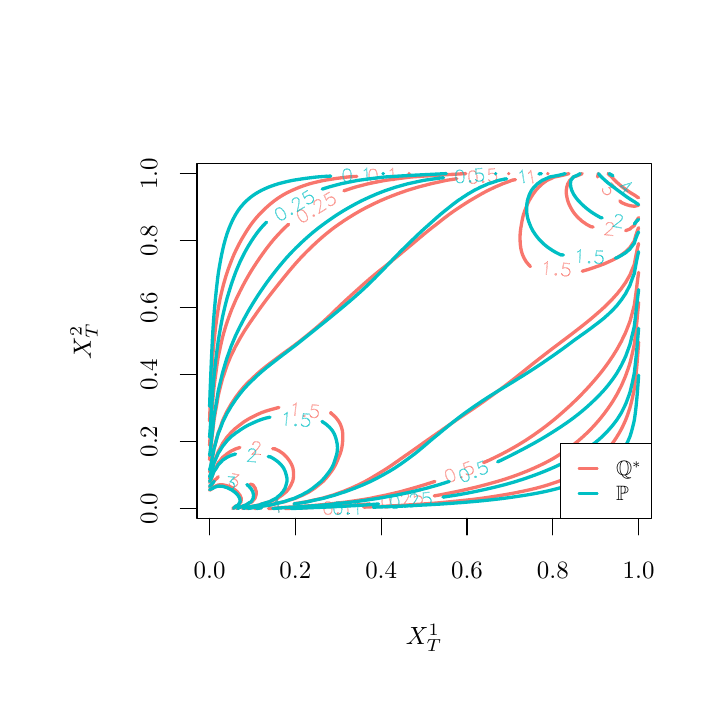
\begin{tikzpicture}[x=1pt,y=1pt]
\definecolor{fillColor}{RGB}{255,255,255}
\path[use as bounding box,fill=fillColor,fill opacity=0.00] (0,0) rectangle (238.49,238.49);
\begin{scope}
\path[clip] (  0.00,  0.00) rectangle (238.49,238.49);
\definecolor{drawColor}{RGB}{0,0,0}

\node[text=drawColor,anchor=base,inner sep=0pt, outer sep=0pt, scale=  0.90] at (143.25, 15.60) {$X^1_T$};

\node[text=drawColor,rotate= 90.00,anchor=base,inner sep=0pt, outer sep=0pt, scale=  0.90] at ( 22.80,125.25) {$X^2_T$};
\end{scope}
\begin{scope}
\path[clip] ( 61.20, 61.20) rectangle (225.29,189.29);
\definecolor{drawColor}{RGB}{248,118,109}

\path[draw=drawColor,line width= 1.2pt,line join=round,line cap=round] ( 65.73, 96.33) --
	( 65.73, 96.52) --
	( 65.77, 97.74) --
	( 65.82, 98.96) --
	( 65.87,100.19) --
	( 65.92,101.41) --
	( 65.97,102.63) --
	( 66.02,103.85) --
	( 66.07,105.08) --
	( 66.12,106.30) --
	( 66.17,107.52) --
	( 66.22,108.74) --
	( 66.29,109.97) --
	( 66.35,111.19) --
	( 66.42,112.41) --
	( 66.49,113.63) --
	( 66.56,114.85) --
	( 66.63,116.08) --
	( 66.70,117.30) --
	( 66.78,118.52) --
	( 66.87,119.74) --
	( 66.97,120.97) --
	( 67.08,122.19) --
	( 67.19,123.41) --
	( 67.29,124.55) --
	( 67.30,124.63) --
	( 67.42,125.86) --
	( 67.55,127.08) --
	( 67.68,128.30) --
	( 67.82,129.52) --
	( 67.97,130.75) --
	( 68.13,131.97) --
	( 68.30,133.19) --
	( 68.48,134.41) --
	( 68.66,135.64) --
	( 68.85,136.86) --
	( 68.86,136.91) --
	( 69.06,138.08) --
	( 69.29,139.30) --
	( 69.53,140.53) --
	( 69.80,141.75) --
	( 70.08,142.97) --
	( 70.38,144.19) --
	( 70.43,144.40) --
	( 70.69,145.42) --
	( 71.03,146.64) --
	( 71.38,147.86) --
	( 71.76,149.08) --
	( 71.99,149.81) --
	( 72.16,150.31) --
	( 72.58,151.53) --
	( 73.03,152.75) --
	( 73.50,153.97) --
	( 73.56,154.12) --
	( 73.99,155.20) --
	( 74.50,156.42) --
	( 75.06,157.64) --
	( 75.12,157.78) --
	( 75.64,158.86) --
	( 76.26,160.08) --
	( 76.69,160.88) --
	( 76.92,161.31) --
	( 77.61,162.53) --
	( 78.26,163.60) --
	( 78.35,163.75) --
	( 79.10,164.97) --
	( 79.82,166.08) --
	( 79.90,166.20) --
	( 80.75,167.42) --
	( 81.39,168.28) --
	( 81.67,168.64) --
	( 82.68,169.86) --
	( 82.95,170.17) --
	( 83.78,171.09) --
	( 84.52,171.85) --
	( 84.98,172.31) --
	( 86.09,173.36) --
	( 86.27,173.53) --
	( 87.65,174.75) --
	( 87.66,174.75) --
	( 89.18,175.98) --
	( 89.22,176.00) --
	( 90.78,177.10) --
	( 90.94,177.20) --
	( 92.35,178.07) --
	( 92.97,178.42) --
	( 93.92,178.92) --
	( 95.42,179.64) --
	( 95.48,179.67) --
	( 97.05,180.35) --
	( 98.32,180.87) --
	( 98.61,180.97) --
	(100.18,181.53) --
	(101.75,182.03) --
	(101.92,182.09) --
	(103.31,182.45) --
	(104.88,182.83) --
	(106.44,183.17) --
	(107.14,183.31) --
	(108.01,183.46) --
	(109.58,183.71) --
	(111.14,183.95) --
	(112.71,184.17) --
	(114.27,184.37) --
	(115.65,184.53) --
	(115.84,184.55) --
	(117.41,184.67);

\path[draw=drawColor,line width= 1.2pt,line join=round,line cap=round] (137.76,185.75) --
	(137.85,185.76);

\path[draw=drawColor,line width= 1.2pt,line join=round,line cap=round] (117.41,184.67) -- (118.93,184.75);

\path[draw=drawColor,line width= 0.1pt,line join=round,line cap=round] (124.47,187.44) -- (123.81,187.17);

\path[draw=drawColor,line width= 0.1pt,line join=round,line cap=round] (123.81,187.17) -- (123.39,186.47);

\path[draw=drawColor,line width= 0.1pt,line join=round,line cap=round] (123.39,186.47) -- (123.22,185.32);

\path[draw=drawColor,line width= 0.1pt,line join=round,line cap=round] (123.22,185.32) -- (123.26,184.64);

\path[draw=drawColor,line width= 0.1pt,line join=round,line cap=round] (123.26,184.64) -- (123.54,183.52);

\path[draw=drawColor,line width= 0.1pt,line join=round,line cap=round] (123.54,183.52) -- (124.03,182.86);

\path[draw=drawColor,line width= 0.1pt,line join=round,line cap=round] (124.03,182.86) -- (124.73,182.67);

\path[draw=drawColor,line width= 0.1pt,line join=round,line cap=round] (124.73,182.67) -- (125.18,182.69);

\path[draw=drawColor,line width= 0.1pt,line join=round,line cap=round] (125.18,182.69) -- (125.85,182.96);

\path[draw=drawColor,line width= 0.1pt,line join=round,line cap=round] (125.85,182.96) -- (126.27,183.66);

\path[draw=drawColor,line width= 0.1pt,line join=round,line cap=round] (126.27,183.66) -- (126.43,184.81);

\path[draw=drawColor,line width= 0.1pt,line join=round,line cap=round] (126.43,184.81) -- (126.40,185.49);

\path[draw=drawColor,line width= 0.1pt,line join=round,line cap=round] (126.40,185.49) -- (126.11,186.61);

\path[draw=drawColor,line width= 0.1pt,line join=round,line cap=round] (126.11,186.61) -- (125.62,187.27);

\path[draw=drawColor,line width= 0.1pt,line join=round,line cap=round] (125.62,187.27) -- (124.93,187.46);

\path[draw=drawColor,line width= 0.1pt,line join=round,line cap=round] (124.93,187.46) -- (124.47,187.44);

\path[draw=drawColor,line width= 0.1pt,line join=round,line cap=round] (124.03,187.19) -- (123.62,186.48);

\path[draw=drawColor,line width= 0.1pt,line join=round,line cap=round] (123.62,186.48) -- (123.45,185.33);

\path[draw=drawColor,line width= 0.1pt,line join=round,line cap=round] (123.45,185.33) -- (123.48,184.65);

\path[draw=drawColor,line width= 0.1pt,line join=round,line cap=round] (123.48,184.65) -- (123.77,183.53);

\path[draw=drawColor,line width= 0.1pt,line join=round,line cap=round] (123.77,183.53) -- (124.26,182.87);

\path[draw=drawColor,line width= 0.1pt,line join=round,line cap=round] (124.02,183.09) -- (124.72,182.90);

\path[draw=drawColor,line width= 0.1pt,line join=round,line cap=round] (124.72,182.90) -- (125.17,182.92);

\path[draw=drawColor,line width= 0.1pt,line join=round,line cap=round] (125.17,182.92) -- (125.84,183.18);

\path[draw=drawColor,line width= 0.1pt,line join=round,line cap=round] (125.62,182.95) -- (126.04,183.65);

\path[draw=drawColor,line width= 0.1pt,line join=round,line cap=round] (126.04,183.65) -- (126.21,184.80);

\path[draw=drawColor,line width= 0.1pt,line join=round,line cap=round] (126.21,184.80) -- (126.17,185.48);

\path[draw=drawColor,line width= 0.1pt,line join=round,line cap=round] (126.17,185.48) -- (125.88,186.60);

\path[draw=drawColor,line width= 0.1pt,line join=round,line cap=round] (125.88,186.60) -- (125.39,187.26);

\path[draw=drawColor,line width= 0.1pt,line join=round,line cap=round] (125.63,187.04) -- (124.94,187.23);

\path[draw=drawColor,line width= 0.1pt,line join=round,line cap=round] (124.94,187.23) -- (124.49,187.21);

\path[draw=drawColor,line width= 0.1pt,line join=round,line cap=round] (124.49,187.21) -- (123.82,186.95);

\path[draw=drawColor,line width= 0.1pt,line join=round,line cap=round] (128.32,183.54) -- (128.11,183.31);

\path[draw=drawColor,line width= 0.1pt,line join=round,line cap=round] (128.11,183.31) -- (128.12,183.08);

\path[draw=drawColor,line width= 0.1pt,line join=round,line cap=round] (128.12,183.08) -- (128.36,182.86);

\path[draw=drawColor,line width= 0.1pt,line join=round,line cap=round] (128.36,182.86) -- (128.59,182.88);

\path[draw=drawColor,line width= 0.1pt,line join=round,line cap=round] (128.59,182.88) -- (128.80,183.11);

\path[draw=drawColor,line width= 0.1pt,line join=round,line cap=round] (128.80,183.11) -- (128.79,183.34);

\path[draw=drawColor,line width= 0.1pt,line join=round,line cap=round] (128.79,183.34) -- (128.55,183.56);

\path[draw=drawColor,line width= 0.1pt,line join=round,line cap=round] (128.55,183.56) -- (128.32,183.54);

\path[draw=drawColor,line width= 0.1pt,line join=round,line cap=round] (128.33,183.32) -- (128.35,183.09);

\path[draw=drawColor,line width= 0.1pt,line join=round,line cap=round] (128.35,183.09) -- (128.57,183.10);

\path[draw=drawColor,line width= 0.1pt,line join=round,line cap=round] (128.57,183.10) -- (128.56,183.33);

\path[draw=drawColor,line width= 0.1pt,line join=round,line cap=round] (128.56,183.33) -- (128.33,183.32);

\path[draw=drawColor,line width= 0.1pt,line join=round,line cap=round] (130.88,186.87) -- (131.32,187.12);

\path[draw=drawColor,line width= 0.1pt,line join=round,line cap=round] (131.32,187.12) -- (131.96,187.83);

\path[draw=drawColor,line width= 0.1pt,line join=round,line cap=round] (131.96,187.83) -- (132.22,183.07);

\path[draw=drawColor,line width= 0.1pt,line join=round,line cap=round] (130.88,186.87) -- (130.89,186.64);

\path[draw=drawColor,line width= 0.1pt,line join=round,line cap=round] (130.89,186.64) -- (131.33,186.89);

\path[draw=drawColor,line width= 0.1pt,line join=round,line cap=round] (131.33,186.89) -- (131.76,187.37);

\path[draw=drawColor,line width= 0.1pt,line join=round,line cap=round] (131.76,187.37) -- (131.99,183.06);

\path[draw=drawColor,line width= 0.1pt,line join=round,line cap=round] (131.99,183.06) -- (132.22,183.07);

\path[draw=drawColor,line width= 1.2pt,line join=round,line cap=round] (122.10, 65.26) --
	(123.67, 65.32) --
	(125.24, 65.39) --
	(126.80, 65.46) --
	(128.37, 65.53) --
	(129.93, 65.60) --
	(131.50, 65.67) --
	(133.07, 65.75) --
	(134.63, 65.84) --
	(136.20, 65.94) --
	(136.42, 65.96) --
	(137.76, 66.04) --
	(139.33, 66.14) --
	(140.90, 66.24) --
	(142.46, 66.35) --
	(144.03, 66.45) --
	(145.59, 66.56) --
	(147.16, 66.68) --
	(148.73, 66.81) --
	(150.29, 66.95) --
	(151.86, 67.11) --
	(152.62, 67.18) --
	(153.42, 67.26) --
	(154.99, 67.41) --
	(156.56, 67.57) --
	(158.12, 67.73) --
	(159.69, 67.90) --
	(161.25, 68.08) --
	(162.82, 68.28) --
	(163.75, 68.40) --
	(164.39, 68.49) --
	(165.95, 68.71) --
	(167.52, 68.94) --
	(169.08, 69.18) --
	(170.65, 69.44) --
	(171.78, 69.62) --
	(172.22, 69.70) --
	(173.78, 69.97) --
	(175.35, 70.25) --
	(176.91, 70.56) --
	(178.30, 70.85) --
	(178.48, 70.88) --
	(180.05, 71.21) --
	(181.61, 71.56) --
	(183.18, 71.94) --
	(183.71, 72.07) --
	(184.74, 72.34) --
	(186.31, 72.77) --
	(187.88, 73.24) --
	(188.03, 73.29) --
	(189.44, 73.74) --
	(191.01, 74.28) --
	(191.66, 74.51) --
	(192.57, 74.85) --
	(194.14, 75.45) --
	(194.83, 75.74) --
	(195.71, 76.11) --
	(197.27, 76.83) --
	(197.54, 76.96) --
	(198.84, 77.63) --
	(199.82, 78.18) --
	(200.40, 78.53) --
	(201.79, 79.40) --
	(201.97, 79.53) --
	(203.54, 80.62) --
	(203.55, 80.63) --
	(205.10, 81.82) --
	(205.14, 81.85) --
	(206.57, 83.07) --
	(206.67, 83.16) --
	(207.87, 84.29) --
	(208.23, 84.66) --
	(209.04, 85.52) --
	(209.80, 86.38) --
	(210.10, 86.74) --
	(211.06, 87.96) --
	(211.37, 88.38) --
	(211.94, 89.18) --
	(212.75, 90.41) --
	(212.93, 90.69) --
	(213.51, 91.63) --
	(214.21, 92.85) --
	(214.50, 93.38) --
	(214.85, 94.07) --
	(215.44, 95.30) --
	(215.99, 96.52) --
	(216.06, 96.70) --
	(216.47, 97.74) --
	(216.91, 98.96) --
	(217.32,100.19) --
	(217.63,101.15) --
	(217.70,101.41) --
	(218.02,102.63) --
	(218.32,103.85) --
	(218.60,105.08) --
	(218.86,106.30) --
	(219.11,107.52) --
	(219.20,107.97) --
	(219.30,108.74) --
	(219.46,109.97) --
	(219.61,111.19) --
	(219.74,112.41) --
	(219.87,113.63) --
	(219.98,114.85) --
	(220.10,116.08) --
	(220.20,117.30) --
	(220.30,118.52) --
	(220.40,119.74) --
	(220.50,120.97) --
	(220.58,122.19) --
	(220.67,123.41) --
	(220.75,124.63) --
	(220.76,124.90);

\path[draw=drawColor,line width= 1.2pt,line join=round,line cap=round] (121.45, 65.24) -- (122.10, 65.26);

\path[draw=drawColor,line width= 0.1pt,line join=round,line cap=round] (108.21, 67.27) -- (107.54, 67.03);

\path[draw=drawColor,line width= 0.1pt,line join=round,line cap=round] (107.54, 67.03) -- (107.10, 66.33);

\path[draw=drawColor,line width= 0.1pt,line join=round,line cap=round] (107.10, 66.33) -- (106.90, 65.19);

\path[draw=drawColor,line width= 0.1pt,line join=round,line cap=round] (106.90, 65.19) -- (106.92, 64.51);

\path[draw=drawColor,line width= 0.1pt,line join=round,line cap=round] (106.92, 64.51) -- (107.18, 63.38);

\path[draw=drawColor,line width= 0.1pt,line join=round,line cap=round] (107.18, 63.38) -- (107.65, 62.71);

\path[draw=drawColor,line width= 0.1pt,line join=round,line cap=round] (107.65, 62.71) -- (108.34, 62.50);

\path[draw=drawColor,line width= 0.1pt,line join=round,line cap=round] (108.34, 62.50) -- (108.79, 62.51);

\path[draw=drawColor,line width= 0.1pt,line join=round,line cap=round] (108.79, 62.51) -- (109.47, 62.76);

\path[draw=drawColor,line width= 0.1pt,line join=round,line cap=round] (109.47, 62.76) -- (109.91, 63.45);

\path[draw=drawColor,line width= 0.1pt,line join=round,line cap=round] (109.91, 63.45) -- (110.10, 64.60);

\path[draw=drawColor,line width= 0.1pt,line join=round,line cap=round] (110.10, 64.60) -- (110.08, 65.28);

\path[draw=drawColor,line width= 0.1pt,line join=round,line cap=round] (110.08, 65.28) -- (109.83, 66.41);

\path[draw=drawColor,line width= 0.1pt,line join=round,line cap=round] (109.83, 66.41) -- (109.35, 67.08);

\path[draw=drawColor,line width= 0.1pt,line join=round,line cap=round] (109.35, 67.08) -- (108.67, 67.29);

\path[draw=drawColor,line width= 0.1pt,line join=round,line cap=round] (108.67, 67.29) -- (108.21, 67.27);

\path[draw=drawColor,line width= 0.1pt,line join=round,line cap=round] (107.76, 67.03) -- (107.33, 66.34);

\path[draw=drawColor,line width= 0.1pt,line join=round,line cap=round] (107.33, 66.34) -- (107.13, 65.20);

\path[draw=drawColor,line width= 0.1pt,line join=round,line cap=round] (107.13, 65.20) -- (107.15, 64.52);

\path[draw=drawColor,line width= 0.1pt,line join=round,line cap=round] (107.15, 64.52) -- (107.41, 63.39);

\path[draw=drawColor,line width= 0.1pt,line join=round,line cap=round] (107.41, 63.39) -- (107.88, 62.72);

\path[draw=drawColor,line width= 0.1pt,line join=round,line cap=round] (107.65, 62.94) -- (108.33, 62.73);

\path[draw=drawColor,line width= 0.1pt,line join=round,line cap=round] (108.33, 62.73) -- (108.79, 62.74);

\path[draw=drawColor,line width= 0.1pt,line join=round,line cap=round] (108.79, 62.74) -- (109.46, 62.99);

\path[draw=drawColor,line width= 0.1pt,line join=round,line cap=round] (109.24, 62.75) -- (109.68, 63.45);

\path[draw=drawColor,line width= 0.1pt,line join=round,line cap=round] (109.68, 63.45) -- (109.88, 64.59);

\path[draw=drawColor,line width= 0.1pt,line join=round,line cap=round] (109.88, 64.59) -- (109.86, 65.27);

\path[draw=drawColor,line width= 0.1pt,line join=round,line cap=round] (109.86, 65.27) -- (109.60, 66.40);

\path[draw=drawColor,line width= 0.1pt,line join=round,line cap=round] (109.60, 66.40) -- (109.13, 67.07);

\path[draw=drawColor,line width= 0.1pt,line join=round,line cap=round] (109.36, 66.85) -- (108.67, 67.06);

\path[draw=drawColor,line width= 0.1pt,line join=round,line cap=round] (108.67, 67.06) -- (108.22, 67.05);

\path[draw=drawColor,line width= 0.1pt,line join=round,line cap=round] (108.22, 67.05) -- (107.54, 66.80);

\path[draw=drawColor,line width= 0.1pt,line join=round,line cap=round] (111.96, 63.28) -- (111.74, 63.05);

\path[draw=drawColor,line width= 0.1pt,line join=round,line cap=round] (111.74, 63.05) -- (111.74, 62.82);

\path[draw=drawColor,line width= 0.1pt,line join=round,line cap=round] (111.74, 62.82) -- (111.98, 62.60);

\path[draw=drawColor,line width= 0.1pt,line join=round,line cap=round] (111.98, 62.60) -- (112.20, 62.61);

\path[draw=drawColor,line width= 0.1pt,line join=round,line cap=round] (112.20, 62.61) -- (112.42, 62.84);

\path[draw=drawColor,line width= 0.1pt,line join=round,line cap=round] (112.42, 62.84) -- (112.42, 63.07);

\path[draw=drawColor,line width= 0.1pt,line join=round,line cap=round] (112.42, 63.07) -- (112.18, 63.29);

\path[draw=drawColor,line width= 0.1pt,line join=round,line cap=round] (112.18, 63.29) -- (111.96, 63.28);

\path[draw=drawColor,line width= 0.1pt,line join=round,line cap=round] (111.96, 63.05) -- (111.97, 62.83);

\path[draw=drawColor,line width= 0.1pt,line join=round,line cap=round] (111.97, 62.83) -- (112.20, 62.83);

\path[draw=drawColor,line width= 0.1pt,line join=round,line cap=round] (112.20, 62.83) -- (112.19, 63.06);

\path[draw=drawColor,line width= 0.1pt,line join=round,line cap=round] (112.19, 63.06) -- (111.96, 63.05);

\path[draw=drawColor,line width= 0.1pt,line join=round,line cap=round] (114.60, 66.53) -- (115.05, 66.77);

\path[draw=drawColor,line width= 0.1pt,line join=round,line cap=round] (115.05, 66.77) -- (115.71, 67.47);

\path[draw=drawColor,line width= 0.1pt,line join=round,line cap=round] (115.71, 67.47) -- (115.84, 62.70);

\path[draw=drawColor,line width= 0.1pt,line join=round,line cap=round] (114.60, 66.53) -- (114.60, 66.31);

\path[draw=drawColor,line width= 0.1pt,line join=round,line cap=round] (114.60, 66.31) -- (115.05, 66.55);

\path[draw=drawColor,line width= 0.1pt,line join=round,line cap=round] (115.05, 66.55) -- (115.49, 67.01);

\path[draw=drawColor,line width= 0.1pt,line join=round,line cap=round] (115.49, 67.01) -- (115.61, 62.70);

\path[draw=drawColor,line width= 0.1pt,line join=round,line cap=round] (115.61, 62.70) -- (115.84, 62.70);

\path[draw=drawColor,line width= 1.2pt,line join=round,line cap=round] ( 65.73, 87.53) --
	( 65.76, 87.96) --
	( 65.83, 89.18) --
	( 65.91, 90.41) --
	( 66.00, 91.63) --
	( 66.09, 92.85) --
	( 66.17, 94.07) --
	( 66.25, 95.30) --
	( 66.33, 96.52) --
	( 66.40, 97.74) --
	( 66.49, 98.96) --
	( 66.59,100.19) --
	( 66.69,101.41) --
	( 66.80,102.63) --
	( 66.90,103.85) --
	( 67.00,105.08) --
	( 67.11,106.30) --
	( 67.23,107.52) --
	( 67.29,108.16) --
	( 67.36,108.74) --
	( 67.52,109.97) --
	( 67.67,111.19) --
	( 67.83,112.41) --
	( 67.99,113.63) --
	( 68.15,114.85) --
	( 68.32,116.08) --
	( 68.50,117.30) --
	( 68.69,118.52) --
	( 68.86,119.51) --
	( 68.91,119.74) --
	( 69.17,120.97) --
	( 69.43,122.19) --
	( 69.69,123.41) --
	( 69.96,124.63) --
	( 70.24,125.86) --
	( 70.43,126.64) --
	( 70.55,127.08) --
	( 70.88,128.30) --
	( 71.24,129.52) --
	( 71.61,130.75) --
	( 71.99,131.92) --
	( 72.01,131.97) --
	( 72.44,133.19) --
	( 72.88,134.41) --
	( 73.33,135.64) --
	( 73.56,136.24) --
	( 73.81,136.86) --
	( 74.32,138.08) --
	( 74.85,139.30) --
	( 75.12,139.93) --
	( 75.40,140.53) --
	( 75.99,141.75) --
	( 76.59,142.97) --
	( 76.69,143.18) --
	( 77.21,144.19) --
	( 77.84,145.42) --
	( 78.26,146.20) --
	( 78.50,146.64) --
	( 79.18,147.86) --
	( 79.82,148.98) --
	( 79.88,149.08) --
	( 80.61,150.31) --
	( 81.37,151.53) --
	( 81.39,151.55) --
	( 82.16,152.75) --
	( 82.95,153.95) --
	( 82.97,153.97) --
	( 83.80,155.20) --
	( 84.52,156.22) --
	( 84.66,156.42) --
	( 85.54,157.64) --
	( 86.09,158.39) --
	( 86.44,158.86) --
	( 87.39,160.08) --
	( 87.65,160.42) --
	( 88.37,161.31) --
	( 89.22,162.30) --
	( 89.42,162.53) --
	( 90.53,163.75) --
	( 90.78,164.02) --
	( 91.70,164.97) --
	( 92.35,165.63) --
	( 92.92,166.20) --
	( 93.92,167.15) --
	( 94.21,167.42);

\path[draw=drawColor,line width= 1.2pt,line join=round,line cap=round] (114.27,179.54) --
	(114.56,179.64) --
	(115.84,180.07) --
	(117.41,180.57) --
	(118.39,180.87) --
	(118.97,181.03) --
	(120.54,181.44) --
	(122.10,181.84) --
	(123.09,182.09) --
	(123.67,182.21) --
	(125.24,182.54) --
	(126.80,182.85) --
	(128.37,183.15) --
	(129.26,183.31) --
	(129.93,183.41) --
	(131.50,183.62) --
	(133.07,183.83) --
	(134.63,184.04) --
	(136.20,184.24) --
	(137.76,184.44) --
	(138.56,184.53) --
	(139.33,184.59) --
	(140.90,184.70) --
	(142.46,184.80) --
	(144.03,184.91) --
	(145.59,185.00) --
	(147.16,185.10) --
	(148.73,185.20) --
	(150.29,185.30) --
	(151.86,185.39) --
	(153.42,185.48) --
	(154.99,185.57) --
	(156.56,185.66) --
	(158.12,185.74) --
	(158.33,185.76);

\path[draw=drawColor,line width= 1.2pt,line join=round,line cap=round] ( 94.21,167.42) -- ( 94.23,167.44);

\path[draw=drawColor,line width= 0.1pt,line join=round,line cap=round] ( 97.86,172.42) -- ( 97.40,171.87);

\path[draw=drawColor,line width= 0.1pt,line join=round,line cap=round] ( 97.40,171.87) -- ( 97.36,171.05);

\path[draw=drawColor,line width= 0.1pt,line join=round,line cap=round] ( 97.36,171.05) -- ( 97.75,169.96);

\path[draw=drawColor,line width= 0.1pt,line join=round,line cap=round] ( 97.75,169.96) -- ( 98.11,169.38);

\path[draw=drawColor,line width= 0.1pt,line join=round,line cap=round] ( 98.11,169.38) -- ( 98.89,168.52);

\path[draw=drawColor,line width= 0.1pt,line join=round,line cap=round] ( 98.89,168.52) -- ( 99.63,168.17);

\path[draw=drawColor,line width= 0.1pt,line join=round,line cap=round] ( 99.63,168.17) -- (100.33,168.33);

\path[draw=drawColor,line width= 0.1pt,line join=round,line cap=round] (100.33,168.33) -- (100.72,168.57);

\path[draw=drawColor,line width= 0.1pt,line join=round,line cap=round] (100.72,168.57) -- (101.19,169.11);

\path[draw=drawColor,line width= 0.1pt,line join=round,line cap=round] (101.19,169.11) -- (101.22,169.93);

\path[draw=drawColor,line width= 0.1pt,line join=round,line cap=round] (101.22,169.93) -- (100.83,171.02);

\path[draw=drawColor,line width= 0.1pt,line join=round,line cap=round] (100.83,171.02) -- (100.48,171.61);

\path[draw=drawColor,line width= 0.1pt,line join=round,line cap=round] (100.48,171.61) -- ( 99.70,172.46);

\path[draw=drawColor,line width= 0.1pt,line join=round,line cap=round] ( 99.70,172.46) -- ( 98.95,172.81);

\path[draw=drawColor,line width= 0.1pt,line join=round,line cap=round] ( 98.95,172.81) -- ( 98.25,172.65);

\path[draw=drawColor,line width= 0.1pt,line join=round,line cap=round] ( 98.25,172.65) -- ( 97.86,172.42);

\path[draw=drawColor,line width= 0.1pt,line join=round,line cap=round] ( 97.59,171.99) -- ( 97.56,171.17);

\path[draw=drawColor,line width= 0.1pt,line join=round,line cap=round] ( 97.56,171.17) -- ( 97.95,170.08);

\path[draw=drawColor,line width= 0.1pt,line join=round,line cap=round] ( 97.95,170.08) -- ( 98.30,169.50);

\path[draw=drawColor,line width= 0.1pt,line join=round,line cap=round] ( 98.30,169.50) -- ( 99.08,168.64);

\path[draw=drawColor,line width= 0.1pt,line join=round,line cap=round] ( 99.08,168.64) -- ( 99.83,168.29);

\path[draw=drawColor,line width= 0.1pt,line join=round,line cap=round] ( 99.51,168.37) -- (100.21,168.53);

\path[draw=drawColor,line width= 0.1pt,line join=round,line cap=round] (100.21,168.53) -- (100.60,168.76);

\path[draw=drawColor,line width= 0.1pt,line join=round,line cap=round] (100.60,168.76) -- (101.07,169.31);

\path[draw=drawColor,line width= 0.1pt,line join=round,line cap=round] (100.99,169.00) -- (101.03,169.82);

\path[draw=drawColor,line width= 0.1pt,line join=round,line cap=round] (101.03,169.82) -- (100.64,170.91);

\path[draw=drawColor,line width= 0.1pt,line join=round,line cap=round] (100.64,170.91) -- (100.28,171.49);

\path[draw=drawColor,line width= 0.1pt,line join=round,line cap=round] (100.28,171.49) -- ( 99.50,172.34);

\path[draw=drawColor,line width= 0.1pt,line join=round,line cap=round] ( 99.50,172.34) -- ( 98.76,172.69);

\path[draw=drawColor,line width= 0.1pt,line join=round,line cap=round] ( 99.07,172.62) -- ( 98.37,172.46);

\path[draw=drawColor,line width= 0.1pt,line join=round,line cap=round] ( 98.37,172.46) -- ( 97.98,172.22);

\path[draw=drawColor,line width= 0.1pt,line join=round,line cap=round] ( 97.98,172.22) -- ( 97.52,171.68);

\path[draw=drawColor,line width= 0.1pt,line join=round,line cap=round] (103.09,170.80) -- (103.01,170.48);

\path[draw=drawColor,line width= 0.1pt,line join=round,line cap=round] (103.01,170.48) -- (103.13,170.29);

\path[draw=drawColor,line width= 0.1pt,line join=round,line cap=round] (103.13,170.29) -- (103.44,170.21);

\path[draw=drawColor,line width= 0.1pt,line join=round,line cap=round] (103.44,170.21) -- (103.64,170.33);

\path[draw=drawColor,line width= 0.1pt,line join=round,line cap=round] (103.64,170.33) -- (103.72,170.64);

\path[draw=drawColor,line width= 0.1pt,line join=round,line cap=round] (103.72,170.64) -- (103.60,170.84);

\path[draw=drawColor,line width= 0.1pt,line join=round,line cap=round] (103.60,170.84) -- (103.29,170.91);

\path[draw=drawColor,line width= 0.1pt,line join=round,line cap=round] (103.29,170.91) -- (103.09,170.80);

\path[draw=drawColor,line width= 0.1pt,line join=round,line cap=round] (103.21,170.60) -- (103.33,170.41);

\path[draw=drawColor,line width= 0.1pt,line join=round,line cap=round] (103.33,170.41) -- (103.52,170.52);

\path[draw=drawColor,line width= 0.1pt,line join=round,line cap=round] (103.52,170.52) -- (103.40,170.72);

\path[draw=drawColor,line width= 0.1pt,line join=round,line cap=round] (103.40,170.72) -- (103.21,170.60);

\path[draw=drawColor,line width= 0.1pt,line join=round,line cap=round] (103.51,174.50) -- (103.39,174.69);

\path[draw=drawColor,line width= 0.1pt,line join=round,line cap=round] (103.39,174.69) -- (103.35,175.20);

\path[draw=drawColor,line width= 0.1pt,line join=round,line cap=round] (103.35,175.20) -- (103.43,175.51);

\path[draw=drawColor,line width= 0.1pt,line join=round,line cap=round] (103.43,175.51) -- (103.70,175.94);

\path[draw=drawColor,line width= 0.1pt,line join=round,line cap=round] (103.70,175.94) -- (104.48,176.41);

\path[draw=drawColor,line width= 0.1pt,line join=round,line cap=round] (104.48,176.41) -- (104.98,176.45);

\path[draw=drawColor,line width= 0.1pt,line join=round,line cap=round] (104.98,176.45) -- (105.30,176.38);

\path[draw=drawColor,line width= 0.1pt,line join=round,line cap=round] (105.30,176.38) -- (105.73,176.10);

\path[draw=drawColor,line width= 0.1pt,line join=round,line cap=round] (105.73,176.10) -- (105.96,175.72);

\path[draw=drawColor,line width= 0.1pt,line join=round,line cap=round] (105.96,175.72) -- (106.00,175.21);

\path[draw=drawColor,line width= 0.1pt,line join=round,line cap=round] (106.00,175.21) -- (105.97,174.39);

\path[draw=drawColor,line width= 0.1pt,line join=round,line cap=round] (105.97,174.39) -- (105.39,171.39);

\path[draw=drawColor,line width= 0.1pt,line join=round,line cap=round] (103.51,174.50) -- (103.70,174.62);

\path[draw=drawColor,line width= 0.1pt,line join=round,line cap=round] (103.70,174.62) -- (103.59,174.81);

\path[draw=drawColor,line width= 0.1pt,line join=round,line cap=round] (103.59,174.81) -- (103.55,175.32);

\path[draw=drawColor,line width= 0.1pt,line join=round,line cap=round] (103.55,175.32) -- (103.82,175.75);

\path[draw=drawColor,line width= 0.1pt,line join=round,line cap=round] (103.82,175.75) -- (104.60,176.22);

\path[draw=drawColor,line width= 0.1pt,line join=round,line cap=round] (104.60,176.22) -- (105.10,176.26);

\path[draw=drawColor,line width= 0.1pt,line join=round,line cap=round] (105.10,176.26) -- (105.53,175.99);

\path[draw=drawColor,line width= 0.1pt,line join=round,line cap=round] (105.53,175.99) -- (105.77,175.60);

\path[draw=drawColor,line width= 0.1pt,line join=round,line cap=round] (105.77,175.60) -- (105.81,175.09);

\path[draw=drawColor,line width= 0.1pt,line join=round,line cap=round] (105.81,175.09) -- (105.77,174.27);

\path[draw=drawColor,line width= 0.1pt,line join=round,line cap=round] (105.77,174.27) -- (105.20,171.27);

\path[draw=drawColor,line width= 0.1pt,line join=round,line cap=round] (105.27,171.58) -- (107.80,173.11);

\path[draw=drawColor,line width= 0.1pt,line join=round,line cap=round] (107.80,173.11) -- (107.92,172.92);

\path[draw=drawColor,line width= 0.1pt,line join=round,line cap=round] (105.20,171.27) -- (107.92,172.92);

\path[draw=drawColor,line width= 0.1pt,line join=round,line cap=round] (107.01,177.94) -- (107.87,176.07);

\path[draw=drawColor,line width= 0.1pt,line join=round,line cap=round] (107.32,177.86) -- (107.95,176.38);

\path[draw=drawColor,line width= 0.1pt,line join=round,line cap=round] (107.01,177.94) -- (108.95,179.12);

\path[draw=drawColor,line width= 0.1pt,line join=round,line cap=round] (108.95,179.12) -- (109.07,178.92);

\path[draw=drawColor,line width= 0.1pt,line join=round,line cap=round] (107.32,177.86) -- (109.07,178.92);

\path[draw=drawColor,line width= 0.1pt,line join=round,line cap=round] (107.95,176.38) -- (108.41,176.93);

\path[draw=drawColor,line width= 0.1pt,line join=round,line cap=round] (108.41,176.93) -- (109.00,177.28);

\path[draw=drawColor,line width= 0.1pt,line join=round,line cap=round] (109.00,177.28) -- (109.70,177.44);

\path[draw=drawColor,line width= 0.1pt,line join=round,line cap=round] (109.70,177.44) -- (110.32,177.29);

\path[draw=drawColor,line width= 0.1pt,line join=round,line cap=round] (110.32,177.29) -- (110.87,176.82);

\path[draw=drawColor,line width= 0.1pt,line join=round,line cap=round] (110.87,176.82) -- (111.10,176.43);

\path[draw=drawColor,line width= 0.1pt,line join=round,line cap=round] (111.10,176.43) -- (111.26,175.73);

\path[draw=drawColor,line width= 0.1pt,line join=round,line cap=round] (111.26,175.73) -- (111.11,175.11);

\path[draw=drawColor,line width= 0.1pt,line join=round,line cap=round] (111.11,175.11) -- (110.64,174.56);

\path[draw=drawColor,line width= 0.1pt,line join=round,line cap=round] (110.64,174.56) -- (110.06,174.21);

\path[draw=drawColor,line width= 0.1pt,line join=round,line cap=round] (110.06,174.21) -- (109.36,174.05);

\path[draw=drawColor,line width= 0.1pt,line join=round,line cap=round] (109.36,174.05) -- (109.05,174.13);

\path[draw=drawColor,line width= 0.1pt,line join=round,line cap=round] (109.05,174.13) -- (108.62,174.40);

\path[draw=drawColor,line width= 0.1pt,line join=round,line cap=round] (108.62,174.40) -- (108.81,174.52);

\path[draw=drawColor,line width= 0.1pt,line join=round,line cap=round] (107.87,176.07) -- (108.06,176.19);

\path[draw=drawColor,line width= 0.1pt,line join=round,line cap=round] (108.06,176.19) -- (108.34,176.62);

\path[draw=drawColor,line width= 0.1pt,line join=round,line cap=round] (108.34,176.62) -- (109.11,177.09);

\path[draw=drawColor,line width= 0.1pt,line join=round,line cap=round] (109.11,177.09) -- (109.82,177.25);

\path[draw=drawColor,line width= 0.1pt,line join=round,line cap=round] (109.82,177.25) -- (110.56,176.90);

\path[draw=drawColor,line width= 0.1pt,line join=round,line cap=round] (109.31,177.21) -- (110.13,177.17);

\path[draw=drawColor,line width= 0.1pt,line join=round,line cap=round] (110.13,177.17) -- (110.67,176.70);

\path[draw=drawColor,line width= 0.1pt,line join=round,line cap=round] (110.67,176.70) -- (110.91,176.32);

\path[draw=drawColor,line width= 0.1pt,line join=round,line cap=round] (110.91,176.32) -- (111.07,175.61);

\path[draw=drawColor,line width= 0.1pt,line join=round,line cap=round] (111.07,175.61) -- (110.72,174.87);

\path[draw=drawColor,line width= 0.1pt,line join=round,line cap=round] (111.03,176.12) -- (110.99,175.30);

\path[draw=drawColor,line width= 0.1pt,line join=round,line cap=round] (110.99,175.30) -- (110.52,174.76);

\path[draw=drawColor,line width= 0.1pt,line join=round,line cap=round] (110.52,174.76) -- (109.94,174.40);

\path[draw=drawColor,line width= 0.1pt,line join=round,line cap=round] (109.94,174.40) -- (109.24,174.24);

\path[draw=drawColor,line width= 0.1pt,line join=round,line cap=round] (109.24,174.24) -- (108.81,174.52);

\path[draw=drawColor,line width= 0.1pt,line join=round,line cap=round] (109.75,174.28) -- (108.93,174.32);

\path[draw=drawColor,line width= 1.2pt,line join=round,line cap=round] ( 93.05, 64.74) --
	( 93.92, 64.77) --
	( 95.48, 64.83) --
	( 97.05, 64.88) --
	( 98.61, 64.94) --
	(100.18, 65.02) --
	(101.75, 65.09) --
	(103.31, 65.16) --
	(104.88, 65.22) --
	(106.44, 65.29) --
	(108.01, 65.36) --
	(109.58, 65.44) --
	(111.14, 65.53) --
	(112.71, 65.62) --
	(114.27, 65.72) --
	(115.84, 65.82) --
	(117.41, 65.92) --
	(117.99, 65.96) --
	(118.97, 66.03) --
	(120.54, 66.15) --
	(122.10, 66.27) --
	(123.67, 66.41);

\path[draw=drawColor,line width= 1.2pt,line join=round,line cap=round] (147.16, 69.34) --
	(148.73, 69.61) --
	(148.81, 69.62) --
	(150.29, 69.91) --
	(151.86, 70.22) --
	(153.42, 70.53) --
	(154.96, 70.85) --
	(154.99, 70.85) --
	(156.56, 71.19) --
	(158.12, 71.54) --
	(159.69, 71.90) --
	(160.44, 72.07) --
	(161.25, 72.27) --
	(162.82, 72.65) --
	(164.39, 73.06) --
	(165.30, 73.29) --
	(165.95, 73.47) --
	(167.52, 73.90) --
	(169.08, 74.34) --
	(169.70, 74.51) --
	(170.65, 74.80) --
	(172.22, 75.28) --
	(173.65, 75.74) --
	(173.78, 75.78) --
	(175.35, 76.32) --
	(176.91, 76.88) --
	(177.13, 76.96) --
	(178.48, 77.48) --
	(180.05, 78.10) --
	(180.25, 78.18) --
	(181.61, 78.75) --
	(183.11, 79.40) --
	(183.18, 79.43) --
	(184.74, 80.15) --
	(185.75, 80.63) --
	(186.31, 80.90) --
	(187.88, 81.70) --
	(188.16, 81.85) --
	(189.44, 82.55) --
	(190.34, 83.07) --
	(191.01, 83.48) --
	(192.30, 84.29) --
	(192.57, 84.47) --
	(194.12, 85.52) --
	(194.14, 85.53) --
	(195.71, 86.65) --
	(195.82, 86.74) --
	(197.27, 87.84) --
	(197.43, 87.96) --
	(198.84, 89.10) --
	(198.94, 89.18) --
	(200.34, 90.41) --
	(200.40, 90.46) --
	(201.67, 91.63) --
	(201.97, 91.91) --
	(202.93, 92.85) --
	(203.54, 93.47) --
	(204.11, 94.07) --
	(205.10, 95.14) --
	(205.24, 95.30) --
	(206.30, 96.52) --
	(206.67, 96.95) --
	(207.31, 97.74) --
	(208.23, 98.92) --
	(208.27, 98.96) --
	(209.18,100.19) --
	(209.80,101.05) --
	(210.05,101.41) --
	(210.88,102.63) --
	(211.37,103.37) --
	(211.66,103.85) --
	(212.40,105.08) --
	(212.93,105.99) --
	(213.09,106.30) --
	(213.73,107.52) --
	(214.35,108.74) --
	(214.50,109.05) --
	(214.91,109.97) --
	(215.44,111.19) --
	(215.95,112.41) --
	(216.06,112.69) --
	(216.40,113.63) --
	(216.83,114.85) --
	(217.24,116.08) --
	(217.63,117.27) --
	(217.64,117.30) --
	(217.94,118.52) --
	(218.24,119.74) --
	(218.52,120.97) --
	(218.80,122.19) --
	(219.06,123.41) --
	(219.20,124.08) --
	(219.27,124.63) --
	(219.42,125.86) --
	(219.56,127.08) --
	(219.70,128.30) --
	(219.84,129.52) --
	(219.97,130.75) --
	(220.10,131.97) --
	(220.22,133.19) --
	(220.33,134.41) --
	(220.44,135.64) --
	(220.55,136.86) --
	(220.66,138.08) --
	(220.76,139.18);

\path[draw=drawColor,line width= 1.2pt,line join=round,line cap=round] (146.90, 69.31) -- (147.16, 69.34);

\path[draw=drawColor,line width= 0.1pt,line join=round,line cap=round] (129.01, 69.48) -- (128.36, 69.17);

\path[draw=drawColor,line width= 0.1pt,line join=round,line cap=round] (128.36, 69.17) -- (128.00, 68.44);

\path[draw=drawColor,line width= 0.1pt,line join=round,line cap=round] (128.00, 68.44) -- (127.91, 67.28);

\path[draw=drawColor,line width= 0.1pt,line join=round,line cap=round] (127.91, 67.28) -- (128.00, 66.61);

\path[draw=drawColor,line width= 0.1pt,line join=round,line cap=round] (128.00, 66.61) -- (128.36, 65.51);

\path[draw=drawColor,line width= 0.1pt,line join=round,line cap=round] (128.36, 65.51) -- (128.90, 64.89);

\path[draw=drawColor,line width= 0.1pt,line join=round,line cap=round] (128.90, 64.89) -- (129.60, 64.75);

\path[draw=drawColor,line width= 0.1pt,line join=round,line cap=round] (129.60, 64.75) -- (130.06, 64.80);

\path[draw=drawColor,line width= 0.1pt,line join=round,line cap=round] (130.06, 64.80) -- (130.70, 65.11);

\path[draw=drawColor,line width= 0.1pt,line join=round,line cap=round] (130.70, 65.11) -- (131.07, 65.85);

\path[draw=drawColor,line width= 0.1pt,line join=round,line cap=round] (131.07, 65.85) -- (131.15, 67.00);

\path[draw=drawColor,line width= 0.1pt,line join=round,line cap=round] (131.15, 67.00) -- (131.07, 67.68);

\path[draw=drawColor,line width= 0.1pt,line join=round,line cap=round] (131.07, 67.68) -- (130.70, 68.78);

\path[draw=drawColor,line width= 0.1pt,line join=round,line cap=round] (130.70, 68.78) -- (130.17, 69.40);

\path[draw=drawColor,line width= 0.1pt,line join=round,line cap=round] (130.17, 69.40) -- (129.46, 69.54);

\path[draw=drawColor,line width= 0.1pt,line join=round,line cap=round] (129.46, 69.54) -- (129.01, 69.48);

\path[draw=drawColor,line width= 0.1pt,line join=round,line cap=round] (128.59, 69.20) -- (128.22, 68.47);

\path[draw=drawColor,line width= 0.1pt,line join=round,line cap=round] (128.22, 68.47) -- (128.14, 67.31);

\path[draw=drawColor,line width= 0.1pt,line join=round,line cap=round] (128.14, 67.31) -- (128.22, 66.64);

\path[draw=drawColor,line width= 0.1pt,line join=round,line cap=round] (128.22, 66.64) -- (128.59, 65.54);

\path[draw=drawColor,line width= 0.1pt,line join=round,line cap=round] (128.59, 65.54) -- (129.12, 64.92);

\path[draw=drawColor,line width= 0.1pt,line join=round,line cap=round] (128.87, 65.11) -- (129.58, 64.97);

\path[draw=drawColor,line width= 0.1pt,line join=round,line cap=round] (129.58, 64.97) -- (130.03, 65.03);

\path[draw=drawColor,line width= 0.1pt,line join=round,line cap=round] (130.03, 65.03) -- (130.68, 65.34);

\path[draw=drawColor,line width= 0.1pt,line join=round,line cap=round] (130.48, 65.08) -- (130.84, 65.82);

\path[draw=drawColor,line width= 0.1pt,line join=round,line cap=round] (130.84, 65.82) -- (130.93, 66.97);

\path[draw=drawColor,line width= 0.1pt,line join=round,line cap=round] (130.93, 66.97) -- (130.85, 67.65);

\path[draw=drawColor,line width= 0.1pt,line join=round,line cap=round] (130.85, 67.65) -- (130.48, 68.75);

\path[draw=drawColor,line width= 0.1pt,line join=round,line cap=round] (130.48, 68.75) -- (129.94, 69.37);

\path[draw=drawColor,line width= 0.1pt,line join=round,line cap=round] (130.20, 69.17) -- (129.49, 69.31);

\path[draw=drawColor,line width= 0.1pt,line join=round,line cap=round] (129.49, 69.31) -- (129.04, 69.26);

\path[draw=drawColor,line width= 0.1pt,line join=round,line cap=round] (129.04, 69.26) -- (128.39, 68.95);

\path[draw=drawColor,line width= 0.1pt,line join=round,line cap=round] (133.13, 65.87) -- (132.93, 65.62);

\path[draw=drawColor,line width= 0.1pt,line join=round,line cap=round] (132.93, 65.62) -- (132.96, 65.39);

\path[draw=drawColor,line width= 0.1pt,line join=round,line cap=round] (132.96, 65.39) -- (133.21, 65.20);

\path[draw=drawColor,line width= 0.1pt,line join=round,line cap=round] (133.21, 65.20) -- (133.44, 65.23);

\path[draw=drawColor,line width= 0.1pt,line join=round,line cap=round] (133.44, 65.23) -- (133.64, 65.48);

\path[draw=drawColor,line width= 0.1pt,line join=round,line cap=round] (133.64, 65.48) -- (133.61, 65.70);

\path[draw=drawColor,line width= 0.1pt,line join=round,line cap=round] (133.61, 65.70) -- (133.35, 65.90);

\path[draw=drawColor,line width= 0.1pt,line join=round,line cap=round] (133.35, 65.90) -- (133.13, 65.87);

\path[draw=drawColor,line width= 0.1pt,line join=round,line cap=round] (133.16, 65.65) -- (133.18, 65.42);

\path[draw=drawColor,line width= 0.1pt,line join=round,line cap=round] (133.18, 65.42) -- (133.41, 65.45);

\path[draw=drawColor,line width= 0.1pt,line join=round,line cap=round] (133.41, 65.45) -- (133.38, 65.68);

\path[draw=drawColor,line width= 0.1pt,line join=round,line cap=round] (133.38, 65.68) -- (133.16, 65.65);

\path[draw=drawColor,line width= 0.1pt,line join=round,line cap=round] (135.02, 69.09) -- (134.99, 69.31);

\path[draw=drawColor,line width= 0.1pt,line join=round,line cap=round] (134.99, 69.31) -- (135.16, 69.79);

\path[draw=drawColor,line width= 0.1pt,line join=round,line cap=round] (135.16, 69.79) -- (135.36, 70.05);

\path[draw=drawColor,line width= 0.1pt,line join=round,line cap=round] (135.36, 70.05) -- (135.78, 70.33);

\path[draw=drawColor,line width= 0.1pt,line join=round,line cap=round] (135.78, 70.33) -- (136.68, 70.44);

\path[draw=drawColor,line width= 0.1pt,line join=round,line cap=round] (136.68, 70.44) -- (137.16, 70.27);

\path[draw=drawColor,line width= 0.1pt,line join=round,line cap=round] (137.16, 70.27) -- (137.41, 70.07);

\path[draw=drawColor,line width= 0.1pt,line join=round,line cap=round] (137.41, 70.07) -- (137.70, 69.65);

\path[draw=drawColor,line width= 0.1pt,line join=round,line cap=round] (137.70, 69.65) -- (137.75, 69.20);

\path[draw=drawColor,line width= 0.1pt,line join=round,line cap=round] (137.75, 69.20) -- (137.58, 68.72);

\path[draw=drawColor,line width= 0.1pt,line join=round,line cap=round] (137.58, 68.72) -- (137.22, 67.99);

\path[draw=drawColor,line width= 0.1pt,line join=round,line cap=round] (137.22, 67.99) -- (135.47, 65.48);

\path[draw=drawColor,line width= 0.1pt,line join=round,line cap=round] (135.02, 69.09) -- (135.24, 69.12);

\path[draw=drawColor,line width= 0.1pt,line join=round,line cap=round] (135.24, 69.12) -- (135.21, 69.34);

\path[draw=drawColor,line width= 0.1pt,line join=round,line cap=round] (135.21, 69.34) -- (135.38, 69.82);

\path[draw=drawColor,line width= 0.1pt,line join=round,line cap=round] (135.38, 69.82) -- (135.81, 70.10);

\path[draw=drawColor,line width= 0.1pt,line join=round,line cap=round] (135.81, 70.10) -- (136.71, 70.21);

\path[draw=drawColor,line width= 0.1pt,line join=round,line cap=round] (136.71, 70.21) -- (137.19, 70.05);

\path[draw=drawColor,line width= 0.1pt,line join=round,line cap=round] (137.19, 70.05) -- (137.47, 69.62);

\path[draw=drawColor,line width= 0.1pt,line join=round,line cap=round] (137.47, 69.62) -- (137.53, 69.17);

\path[draw=drawColor,line width= 0.1pt,line join=round,line cap=round] (137.53, 69.17) -- (137.36, 68.69);

\path[draw=drawColor,line width= 0.1pt,line join=round,line cap=round] (137.36, 68.69) -- (136.99, 67.96);

\path[draw=drawColor,line width= 0.1pt,line join=round,line cap=round] (136.99, 67.96) -- (135.24, 65.45);

\path[draw=drawColor,line width= 0.1pt,line join=round,line cap=round] (135.44, 65.70) -- (138.37, 66.07);

\path[draw=drawColor,line width= 0.1pt,line join=round,line cap=round] (138.37, 66.07) -- (138.40, 65.84);

\path[draw=drawColor,line width= 0.1pt,line join=round,line cap=round] (135.24, 65.45) -- (138.40, 65.84);

\path[draw=drawColor,line width= 0.1pt,line join=round,line cap=round] (139.61, 70.81) -- (139.64, 68.75);

\path[draw=drawColor,line width= 0.1pt,line join=round,line cap=round] (139.87, 70.61) -- (139.84, 69.00);

\path[draw=drawColor,line width= 0.1pt,line join=round,line cap=round] (139.61, 70.81) -- (141.87, 71.09);

\path[draw=drawColor,line width= 0.1pt,line join=round,line cap=round] (141.87, 71.09) -- (141.90, 70.86);

\path[draw=drawColor,line width= 0.1pt,line join=round,line cap=round] (139.87, 70.61) -- (141.90, 70.86);

\path[draw=drawColor,line width= 0.1pt,line join=round,line cap=round] (139.84, 69.00) -- (140.49, 69.31);

\path[draw=drawColor,line width= 0.1pt,line join=round,line cap=round] (140.49, 69.31) -- (141.16, 69.40);

\path[draw=drawColor,line width= 0.1pt,line join=round,line cap=round] (141.16, 69.40) -- (141.87, 69.26);

\path[draw=drawColor,line width= 0.1pt,line join=round,line cap=round] (141.87, 69.26) -- (142.37, 68.86);

\path[draw=drawColor,line width= 0.1pt,line join=round,line cap=round] (142.37, 68.86) -- (142.68, 68.21);

\path[draw=drawColor,line width= 0.1pt,line join=round,line cap=round] (142.68, 68.21) -- (142.74, 67.76);

\path[draw=drawColor,line width= 0.1pt,line join=round,line cap=round] (142.74, 67.76) -- (142.60, 67.06);

\path[draw=drawColor,line width= 0.1pt,line join=round,line cap=round] (142.60, 67.06) -- (142.21, 66.55);

\path[draw=drawColor,line width= 0.1pt,line join=round,line cap=round] (142.21, 66.55) -- (141.56, 66.24);

\path[draw=drawColor,line width= 0.1pt,line join=round,line cap=round] (141.56, 66.24) -- (140.88, 66.15);

\path[draw=drawColor,line width= 0.1pt,line join=round,line cap=round] (140.88, 66.15) -- (140.18, 66.30);

\path[draw=drawColor,line width= 0.1pt,line join=round,line cap=round] (140.18, 66.30) -- (139.92, 66.49);

\path[draw=drawColor,line width= 0.1pt,line join=round,line cap=round] (139.92, 66.49) -- (139.64, 66.92);

\path[draw=drawColor,line width= 0.1pt,line join=round,line cap=round] (139.64, 66.92) -- (139.87, 66.94);

\path[draw=drawColor,line width= 0.1pt,line join=round,line cap=round] (139.64, 68.75) -- (139.87, 68.78);

\path[draw=drawColor,line width= 0.1pt,line join=round,line cap=round] (139.87, 68.78) -- (140.29, 69.06);

\path[draw=drawColor,line width= 0.1pt,line join=round,line cap=round] (140.29, 69.06) -- (141.19, 69.17);

\path[draw=drawColor,line width= 0.1pt,line join=round,line cap=round] (141.19, 69.17) -- (141.90, 69.03);

\path[draw=drawColor,line width= 0.1pt,line join=round,line cap=round] (141.90, 69.03) -- (142.43, 68.41);

\path[draw=drawColor,line width= 0.1pt,line join=round,line cap=round] (141.42, 69.20) -- (142.15, 68.83);

\path[draw=drawColor,line width= 0.1pt,line join=round,line cap=round] (142.15, 68.83) -- (142.46, 68.18);

\path[draw=drawColor,line width= 0.1pt,line join=round,line cap=round] (142.46, 68.18) -- (142.52, 67.73);

\path[draw=drawColor,line width= 0.1pt,line join=round,line cap=round] (142.52, 67.73) -- (142.37, 67.03);

\path[draw=drawColor,line width= 0.1pt,line join=round,line cap=round] (142.37, 67.03) -- (141.75, 66.49);

\path[draw=drawColor,line width= 0.1pt,line join=round,line cap=round] (142.54, 67.51) -- (142.18, 66.77);

\path[draw=drawColor,line width= 0.1pt,line join=round,line cap=round] (142.18, 66.77) -- (141.53, 66.46);

\path[draw=drawColor,line width= 0.1pt,line join=round,line cap=round] (141.53, 66.46) -- (140.85, 66.38);

\path[draw=drawColor,line width= 0.1pt,line join=round,line cap=round] (140.85, 66.38) -- (140.15, 66.52);

\path[draw=drawColor,line width= 0.1pt,line join=round,line cap=round] (140.15, 66.52) -- (139.87, 66.94);

\path[draw=drawColor,line width= 0.1pt,line join=round,line cap=round] (140.63, 66.35) -- (139.89, 66.72);

\path[draw=drawColor,line width= 1.2pt,line join=round,line cap=round] ( 65.73, 82.38) --
	( 65.80, 83.07) --
	( 65.97, 84.29) --
	( 66.12, 85.52) --
	( 66.25, 86.74) --
	( 66.37, 87.96) --
	( 66.48, 89.18) --
	( 66.61, 90.41) --
	( 66.75, 91.63) --
	( 66.90, 92.85) --
	( 67.03, 94.07) --
	( 67.17, 95.30) --
	( 67.29, 96.39) --
	( 67.32, 96.52) --
	( 67.51, 97.74) --
	( 67.71, 98.96) --
	( 67.93,100.19) --
	( 68.15,101.41) --
	( 68.37,102.63) --
	( 68.58,103.85) --
	( 68.79,105.08) --
	( 68.86,105.51) --
	( 69.04,106.30) --
	( 69.33,107.52) --
	( 69.63,108.74) --
	( 69.95,109.97) --
	( 70.28,111.19) --
	( 70.43,111.73) --
	( 70.66,112.41) --
	( 71.07,113.63) --
	( 71.48,114.85) --
	( 71.89,116.08) --
	( 71.99,116.37) --
	( 72.36,117.30) --
	( 72.86,118.52) --
	( 73.37,119.74) --
	( 73.56,120.19) --
	( 73.95,120.97) --
	( 74.56,122.19) --
	( 75.12,123.33) --
	( 75.17,123.41) --
	( 75.85,124.63) --
	( 76.52,125.86) --
	( 76.69,126.17) --
	( 77.23,127.08) --
	( 77.96,128.30) --
	( 78.26,128.79) --
	( 78.73,129.52) --
	( 79.54,130.75) --
	( 79.82,131.18) --
	( 80.37,131.97) --
	( 81.21,133.19) --
	( 81.39,133.45) --
	( 82.07,134.41) --
	( 82.92,135.64) --
	( 82.95,135.68) --
	( 83.80,136.86) --
	( 84.52,137.86) --
	( 84.69,138.08) --
	( 85.59,139.30) --
	( 86.09,139.97) --
	( 86.51,140.53) --
	( 87.45,141.75) --
	( 87.65,142.01) --
	( 88.40,142.97) --
	( 89.22,144.02) --
	( 89.36,144.19) --
	( 90.33,145.42) --
	( 90.78,145.99) --
	( 91.30,146.64) --
	( 92.29,147.86) --
	( 92.35,147.94) --
	( 93.28,149.08) --
	( 93.92,149.86) --
	( 94.29,150.31) --
	( 95.31,151.53) --
	( 95.48,151.73) --
	( 96.36,152.75) --
	( 97.05,153.54) --
	( 97.44,153.97) --
	( 98.56,155.20) --
	( 98.61,155.26) --
	( 99.72,156.42) --
	(100.18,156.89) --
	(100.92,157.64) --
	(101.75,158.45) --
	(102.17,158.86) --
	(103.31,159.96) --
	(103.45,160.08) --
	(104.78,161.31) --
	(104.88,161.40) --
	(106.15,162.53) --
	(106.44,162.78) --
	(107.58,163.75) --
	(108.01,164.10) --
	(109.09,164.97) --
	(109.58,165.36) --
	(110.68,166.20) --
	(111.14,166.53) --
	(112.38,167.42) --
	(112.71,167.65) --
	(114.18,168.64) --
	(114.27,168.71) --
	(115.84,169.72) --
	(116.07,169.86) --
	(117.41,170.69) --
	(118.05,171.09) --
	(118.97,171.62) --
	(120.16,172.31) --
	(120.54,172.52) --
	(122.10,173.36) --
	(122.42,173.53) --
	(123.67,174.16) --
	(124.85,174.75) --
	(125.24,174.93) --
	(126.80,175.66) --
	(127.49,175.98) --
	(128.37,176.35) --
	(129.93,177.01) --
	(130.39,177.20) --
	(131.50,177.64) --
	(133.07,178.24) --
	(133.52,178.42) --
	(134.63,178.81) --
	(136.20,179.36) --
	(137.00,179.64) --
	(137.76,179.88) --
	(139.33,180.36) --
	(140.90,180.82) --
	(141.03,180.87) --
	(142.46,181.24) --
	(144.03,181.65) --
	(145.59,182.06) --
	(145.70,182.09) --
	(147.16,182.41) --
	(148.73,182.75) --
	(150.29,183.10) --
	(151.23,183.31) --
	(151.86,183.41) --
	(153.42,183.65) --
	(154.99,183.90);

\path[draw=drawColor,line width= 1.2pt,line join=round,line cap=round] (173.78,185.75) --
	(173.85,185.76);

\path[draw=drawColor,line width= 1.2pt,line join=round,line cap=round] (154.99,183.90) -- (155.01,183.90);

\path[draw=drawColor,line width= 0.1pt,line join=round,line cap=round] (160.43,186.83) -- (159.77,186.54);

\path[draw=drawColor,line width= 0.1pt,line join=round,line cap=round] (159.77,186.54) -- (159.39,185.81);

\path[draw=drawColor,line width= 0.1pt,line join=round,line cap=round] (159.39,185.81) -- (159.27,184.66);

\path[draw=drawColor,line width= 0.1pt,line join=round,line cap=round] (159.27,184.66) -- (159.34,183.98);

\path[draw=drawColor,line width= 0.1pt,line join=round,line cap=round] (159.34,183.98) -- (159.68,182.87);

\path[draw=drawColor,line width= 0.1pt,line join=round,line cap=round] (159.68,182.87) -- (160.20,182.24);

\path[draw=drawColor,line width= 0.1pt,line join=round,line cap=round] (160.20,182.24) -- (160.90,182.08);

\path[draw=drawColor,line width= 0.1pt,line join=round,line cap=round] (160.90,182.08) -- (161.35,182.13);

\path[draw=drawColor,line width= 0.1pt,line join=round,line cap=round] (161.35,182.13) -- (162.01,182.42);

\path[draw=drawColor,line width= 0.1pt,line join=round,line cap=round] (162.01,182.42) -- (162.39,183.14);

\path[draw=drawColor,line width= 0.1pt,line join=round,line cap=round] (162.39,183.14) -- (162.51,184.29);

\path[draw=drawColor,line width= 0.1pt,line join=round,line cap=round] (162.51,184.29) -- (162.44,184.97);

\path[draw=drawColor,line width= 0.1pt,line join=round,line cap=round] (162.44,184.97) -- (162.10,186.08);

\path[draw=drawColor,line width= 0.1pt,line join=round,line cap=round] (162.10,186.08) -- (161.58,186.72);

\path[draw=drawColor,line width= 0.1pt,line join=round,line cap=round] (161.58,186.72) -- (160.88,186.87);

\path[draw=drawColor,line width= 0.1pt,line join=round,line cap=round] (160.88,186.87) -- (160.43,186.83);

\path[draw=drawColor,line width= 0.1pt,line join=round,line cap=round] (160.00,186.56) -- (159.61,185.84);

\path[draw=drawColor,line width= 0.1pt,line join=round,line cap=round] (159.61,185.84) -- (159.50,184.68);

\path[draw=drawColor,line width= 0.1pt,line join=round,line cap=round] (159.50,184.68) -- (159.57,184.00);

\path[draw=drawColor,line width= 0.1pt,line join=round,line cap=round] (159.57,184.00) -- (159.90,182.90);

\path[draw=drawColor,line width= 0.1pt,line join=round,line cap=round] (159.90,182.90) -- (160.42,182.26);

\path[draw=drawColor,line width= 0.1pt,line join=round,line cap=round] (160.18,182.47) -- (160.88,182.31);

\path[draw=drawColor,line width= 0.1pt,line join=round,line cap=round] (160.88,182.31) -- (161.33,182.35);

\path[draw=drawColor,line width= 0.1pt,line join=round,line cap=round] (161.33,182.35) -- (161.99,182.64);

\path[draw=drawColor,line width= 0.1pt,line join=round,line cap=round] (161.78,182.40) -- (162.17,183.12);

\path[draw=drawColor,line width= 0.1pt,line join=round,line cap=round] (162.17,183.12) -- (162.28,184.27);

\path[draw=drawColor,line width= 0.1pt,line join=round,line cap=round] (162.28,184.27) -- (162.21,184.95);

\path[draw=drawColor,line width= 0.1pt,line join=round,line cap=round] (162.21,184.95) -- (161.88,186.06);

\path[draw=drawColor,line width= 0.1pt,line join=round,line cap=round] (161.88,186.06) -- (161.36,186.69);

\path[draw=drawColor,line width= 0.1pt,line join=round,line cap=round] (161.61,186.49) -- (160.90,186.65);

\path[draw=drawColor,line width= 0.1pt,line join=round,line cap=round] (160.90,186.65) -- (160.45,186.60);

\path[draw=drawColor,line width= 0.1pt,line join=round,line cap=round] (160.45,186.60) -- (159.80,186.31);

\path[draw=drawColor,line width= 0.1pt,line join=round,line cap=round] (164.45,183.12) -- (164.25,182.87);

\path[draw=drawColor,line width= 0.1pt,line join=round,line cap=round] (164.25,182.87) -- (164.27,182.64);

\path[draw=drawColor,line width= 0.1pt,line join=round,line cap=round] (164.27,182.64) -- (164.52,182.44);

\path[draw=drawColor,line width= 0.1pt,line join=round,line cap=round] (164.52,182.44) -- (164.74,182.46);

\path[draw=drawColor,line width= 0.1pt,line join=round,line cap=round] (164.74,182.46) -- (164.95,182.71);

\path[draw=drawColor,line width= 0.1pt,line join=round,line cap=round] (164.95,182.71) -- (164.93,182.93);

\path[draw=drawColor,line width= 0.1pt,line join=round,line cap=round] (164.93,182.93) -- (164.68,183.14);

\path[draw=drawColor,line width= 0.1pt,line join=round,line cap=round] (164.68,183.14) -- (164.45,183.12);

\path[draw=drawColor,line width= 0.1pt,line join=round,line cap=round] (164.47,182.89) -- (164.50,182.66);

\path[draw=drawColor,line width= 0.1pt,line join=round,line cap=round] (164.50,182.66) -- (164.72,182.69);

\path[draw=drawColor,line width= 0.1pt,line join=round,line cap=round] (164.72,182.69) -- (164.70,182.91);

\path[draw=drawColor,line width= 0.1pt,line join=round,line cap=round] (164.70,182.91) -- (164.47,182.89);

\path[draw=drawColor,line width= 0.1pt,line join=round,line cap=round] (166.54,187.43) -- (166.51,185.38);

\path[draw=drawColor,line width= 0.1pt,line join=round,line cap=round] (166.79,187.23) -- (166.72,185.62);

\path[draw=drawColor,line width= 0.1pt,line join=round,line cap=round] (166.54,187.43) -- (168.80,187.66);

\path[draw=drawColor,line width= 0.1pt,line join=round,line cap=round] (168.80,187.66) -- (168.82,187.43);

\path[draw=drawColor,line width= 0.1pt,line join=round,line cap=round] (166.79,187.23) -- (168.82,187.43);

\path[draw=drawColor,line width= 0.1pt,line join=round,line cap=round] (166.72,185.62) -- (167.37,185.92);

\path[draw=drawColor,line width= 0.1pt,line join=round,line cap=round] (167.37,185.92) -- (168.05,185.98);

\path[draw=drawColor,line width= 0.1pt,line join=round,line cap=round] (168.05,185.98) -- (168.75,185.82);

\path[draw=drawColor,line width= 0.1pt,line join=round,line cap=round] (168.75,185.82) -- (169.25,185.42);

\path[draw=drawColor,line width= 0.1pt,line join=round,line cap=round] (169.25,185.42) -- (169.54,184.76);

\path[draw=drawColor,line width= 0.1pt,line join=round,line cap=round] (169.54,184.76) -- (169.59,184.31);

\path[draw=drawColor,line width= 0.1pt,line join=round,line cap=round] (169.59,184.31) -- (169.43,183.61);

\path[draw=drawColor,line width= 0.1pt,line join=round,line cap=round] (169.43,183.61) -- (169.02,183.11);

\path[draw=drawColor,line width= 0.1pt,line join=round,line cap=round] (169.02,183.11) -- (168.36,182.82);

\path[draw=drawColor,line width= 0.1pt,line join=round,line cap=round] (168.36,182.82) -- (167.68,182.75);

\path[draw=drawColor,line width= 0.1pt,line join=round,line cap=round] (167.68,182.75) -- (166.98,182.91);

\path[draw=drawColor,line width= 0.1pt,line join=round,line cap=round] (166.98,182.91) -- (166.73,183.11);

\path[draw=drawColor,line width= 0.1pt,line join=round,line cap=round] (166.73,183.11) -- (166.46,183.54);

\path[draw=drawColor,line width= 0.1pt,line join=round,line cap=round] (166.46,183.54) -- (166.69,183.57);

\path[draw=drawColor,line width= 0.1pt,line join=round,line cap=round] (166.51,185.38) -- (166.74,185.40);

\path[draw=drawColor,line width= 0.1pt,line join=round,line cap=round] (166.74,185.40) -- (167.17,185.67);

\path[draw=drawColor,line width= 0.1pt,line join=round,line cap=round] (167.17,185.67) -- (168.07,185.76);

\path[draw=drawColor,line width= 0.1pt,line join=round,line cap=round] (168.07,185.76) -- (168.77,185.60);

\path[draw=drawColor,line width= 0.1pt,line join=round,line cap=round] (168.77,185.60) -- (169.29,184.96);

\path[draw=drawColor,line width= 0.1pt,line join=round,line cap=round] (168.30,185.78) -- (169.02,185.39);

\path[draw=drawColor,line width= 0.1pt,line join=round,line cap=round] (169.02,185.39) -- (169.31,184.74);

\path[draw=drawColor,line width= 0.1pt,line join=round,line cap=round] (169.31,184.74) -- (169.36,184.29);

\path[draw=drawColor,line width= 0.1pt,line join=round,line cap=round] (169.36,184.29) -- (169.20,183.59);

\path[draw=drawColor,line width= 0.1pt,line join=round,line cap=round] (169.20,183.59) -- (168.57,183.07);

\path[draw=drawColor,line width= 0.1pt,line join=round,line cap=round] (169.38,184.06) -- (169.00,183.34);

\path[draw=drawColor,line width= 0.1pt,line join=round,line cap=round] (169.00,183.34) -- (168.34,183.04);

\path[draw=drawColor,line width= 0.1pt,line join=round,line cap=round] (168.34,183.04) -- (167.66,182.98);

\path[draw=drawColor,line width= 0.1pt,line join=round,line cap=round] (167.66,182.98) -- (166.96,183.14);

\path[draw=drawColor,line width= 0.1pt,line join=round,line cap=round] (166.96,183.14) -- (166.69,183.57);

\path[draw=drawColor,line width= 0.1pt,line join=round,line cap=round] (167.44,182.95) -- (166.71,183.34);

\path[draw=drawColor,line width= 1.2pt,line join=round,line cap=round] ( 87.01, 64.74) --
	( 87.65, 64.77) --
	( 89.22, 64.87) --
	( 90.78, 64.99) --
	( 92.35, 65.10) --
	( 93.92, 65.20) --
	( 95.48, 65.29) --
	( 97.05, 65.38) --
	( 98.61, 65.48) --
	(100.18, 65.60) --
	(101.75, 65.71) --
	(103.31, 65.83) --
	(104.88, 65.95) --
	(104.94, 65.96) --
	(106.44, 66.11) --
	(108.01, 66.27) --
	(109.58, 66.44) --
	(111.14, 66.62) --
	(112.71, 66.80) --
	(114.27, 66.98) --
	(115.84, 67.17) --
	(115.95, 67.18) --
	(117.41, 67.40) --
	(118.97, 67.63) --
	(120.54, 67.87) --
	(122.10, 68.12) --
	(123.67, 68.39) --
	(123.74, 68.40) --
	(125.24, 68.72) --
	(126.80, 69.04) --
	(128.37, 69.36) --
	(129.65, 69.62) --
	(129.93, 69.69) --
	(131.50, 70.06) --
	(133.07, 70.42) --
	(134.63, 70.80) --
	(134.83, 70.85) --
	(136.20, 71.23) --
	(137.76, 71.67) --
	(139.21, 72.07) --
	(139.33, 72.11) --
	(140.90, 72.57) --
	(142.46, 73.04) --
	(143.31, 73.29) --
	(144.03, 73.52) --
	(145.59, 74.02) --
	(147.14, 74.51) --
	(147.16, 74.52);

\path[draw=drawColor,line width= 1.2pt,line join=round,line cap=round] (165.95, 81.82) --
	(166.01, 81.85) --
	(167.52, 82.56) --
	(168.59, 83.07) --
	(169.08, 83.32) --
	(170.65, 84.09) --
	(171.05, 84.29) --
	(172.22, 84.90) --
	(173.38, 85.52) --
	(173.78, 85.74) --
	(175.35, 86.61) --
	(175.58, 86.74) --
	(176.91, 87.51) --
	(177.67, 87.96) --
	(178.48, 88.46) --
	(179.64, 89.18) --
	(180.05, 89.44) --
	(181.51, 90.41) --
	(181.61, 90.47) --
	(183.18, 91.54) --
	(183.30, 91.63) --
	(184.74, 92.65) --
	(185.02, 92.85) --
	(186.31, 93.80) --
	(186.67, 94.07) --
	(187.88, 94.99) --
	(188.26, 95.30) --
	(189.44, 96.23) --
	(189.80, 96.52) --
	(191.01, 97.52) --
	(191.27, 97.74) --
	(192.57, 98.86) --
	(192.69, 98.96) --
	(194.07,100.19) --
	(194.14,100.25) --
	(195.42,101.41) --
	(195.71,101.67) --
	(196.73,102.63) --
	(197.27,103.14) --
	(198.01,103.85) --
	(198.84,104.66) --
	(199.25,105.08) --
	(200.40,106.25) --
	(200.45,106.30) --
	(201.62,107.52) --
	(201.97,107.89) --
	(202.74,108.74) --
	(203.54,109.62) --
	(203.84,109.97) --
	(204.91,111.19) --
	(205.10,111.41) --
	(205.94,112.41) --
	(206.67,113.28) --
	(206.95,113.63) --
	(207.91,114.85) --
	(208.23,115.27) --
	(208.82,116.08) --
	(209.71,117.30) --
	(209.80,117.43) --
	(210.55,118.52) --
	(211.37,119.73) --
	(211.38,119.74) --
	(212.14,120.97) --
	(212.90,122.19) --
	(212.93,122.24) --
	(213.58,123.41) --
	(214.25,124.63) --
	(214.50,125.08) --
	(214.87,125.86) --
	(215.46,127.08) --
	(216.05,128.30) --
	(216.06,128.34) --
	(216.53,129.52) --
	(217.01,130.75) --
	(217.48,131.97) --
	(217.63,132.35) --
	(217.86,133.19) --
	(218.20,134.41) --
	(218.52,135.64) --
	(218.85,136.86) --
	(219.17,138.08) --
	(219.20,138.18) --
	(219.35,139.30) --
	(219.52,140.53) --
	(219.69,141.75) --
	(219.85,142.97) --
	(220.01,144.19) --
	(220.16,145.42) --
	(220.31,146.64) --
	(220.46,147.86) --
	(220.62,149.08) --
	(220.76,150.07);

\path[draw=drawColor,line width= 1.2pt,line join=round,line cap=round] (164.74, 81.35) -- (165.95, 81.82);

\path[draw=drawColor,line width= 0.1pt,line join=round,line cap=round] (151.59, 78.81) -- (151.04, 78.35);

\path[draw=drawColor,line width= 0.1pt,line join=round,line cap=round] (151.04, 78.35) -- (150.86, 77.55);

\path[draw=drawColor,line width= 0.1pt,line join=round,line cap=round] (150.86, 77.55) -- (151.06, 76.40);

\path[draw=drawColor,line width= 0.1pt,line join=round,line cap=round] (151.06, 76.40) -- (151.31, 75.77);

\path[draw=drawColor,line width= 0.1pt,line join=round,line cap=round] (151.31, 75.77) -- (151.93, 74.79);

\path[draw=drawColor,line width= 0.1pt,line join=round,line cap=round] (151.93, 74.79) -- (152.60, 74.32);

\path[draw=drawColor,line width= 0.1pt,line join=round,line cap=round] (152.60, 74.32) -- (153.32, 74.36);

\path[draw=drawColor,line width= 0.1pt,line join=round,line cap=round] (153.32, 74.36) -- (153.74, 74.52);

\path[draw=drawColor,line width= 0.1pt,line join=round,line cap=round] (153.74, 74.52) -- (154.30, 74.98);

\path[draw=drawColor,line width= 0.1pt,line join=round,line cap=round] (154.30, 74.98) -- (154.47, 75.78);

\path[draw=drawColor,line width= 0.1pt,line join=round,line cap=round] (154.47, 75.78) -- (154.27, 76.92);

\path[draw=drawColor,line width= 0.1pt,line join=round,line cap=round] (154.27, 76.92) -- (154.03, 77.56);

\path[draw=drawColor,line width= 0.1pt,line join=round,line cap=round] (154.03, 77.56) -- (153.40, 78.53);

\path[draw=drawColor,line width= 0.1pt,line join=round,line cap=round] (153.40, 78.53) -- (152.73, 79.01);

\path[draw=drawColor,line width= 0.1pt,line join=round,line cap=round] (152.73, 79.01) -- (152.02, 78.97);

\path[draw=drawColor,line width= 0.1pt,line join=round,line cap=round] (152.02, 78.97) -- (151.59, 78.81);

\path[draw=drawColor,line width= 0.1pt,line join=round,line cap=round] (151.25, 78.43) -- (151.07, 77.63);

\path[draw=drawColor,line width= 0.1pt,line join=round,line cap=round] (151.07, 77.63) -- (151.27, 76.49);

\path[draw=drawColor,line width= 0.1pt,line join=round,line cap=round] (151.27, 76.49) -- (151.52, 75.85);

\path[draw=drawColor,line width= 0.1pt,line join=round,line cap=round] (151.52, 75.85) -- (152.14, 74.88);

\path[draw=drawColor,line width= 0.1pt,line join=round,line cap=round] (152.14, 74.88) -- (152.81, 74.40);

\path[draw=drawColor,line width= 0.1pt,line join=round,line cap=round] (152.52, 74.53) -- (153.24, 74.57);

\path[draw=drawColor,line width= 0.1pt,line join=round,line cap=round] (153.24, 74.57) -- (153.66, 74.73);

\path[draw=drawColor,line width= 0.1pt,line join=round,line cap=round] (153.66, 74.73) -- (154.22, 75.19);

\path[draw=drawColor,line width= 0.1pt,line join=round,line cap=round] (154.09, 74.90) -- (154.26, 75.70);

\path[draw=drawColor,line width= 0.1pt,line join=round,line cap=round] (154.26, 75.70) -- (154.06, 76.84);

\path[draw=drawColor,line width= 0.1pt,line join=round,line cap=round] (154.06, 76.84) -- (153.82, 77.48);

\path[draw=drawColor,line width= 0.1pt,line join=round,line cap=round] (153.82, 77.48) -- (153.19, 78.45);

\path[draw=drawColor,line width= 0.1pt,line join=round,line cap=round] (153.19, 78.45) -- (152.52, 78.92);

\path[draw=drawColor,line width= 0.1pt,line join=round,line cap=round] (152.82, 78.79) -- (152.10, 78.76);

\path[draw=drawColor,line width= 0.1pt,line join=round,line cap=round] (152.10, 78.76) -- (151.67, 78.59);

\path[draw=drawColor,line width= 0.1pt,line join=round,line cap=round] (151.67, 78.59) -- (151.12, 78.13);

\path[draw=drawColor,line width= 0.1pt,line join=round,line cap=round] (156.46, 76.31) -- (156.33, 76.02);

\path[draw=drawColor,line width= 0.1pt,line join=round,line cap=round] (156.33, 76.02) -- (156.42, 75.80);

\path[draw=drawColor,line width= 0.1pt,line join=round,line cap=round] (156.42, 75.80) -- (156.71, 75.67);

\path[draw=drawColor,line width= 0.1pt,line join=round,line cap=round] (156.71, 75.67) -- (156.92, 75.76);

\path[draw=drawColor,line width= 0.1pt,line join=round,line cap=round] (156.92, 75.76) -- (157.05, 76.05);

\path[draw=drawColor,line width= 0.1pt,line join=round,line cap=round] (157.05, 76.05) -- (156.97, 76.26);

\path[draw=drawColor,line width= 0.1pt,line join=round,line cap=round] (156.97, 76.26) -- (156.67, 76.39);

\path[draw=drawColor,line width= 0.1pt,line join=round,line cap=round] (156.67, 76.39) -- (156.46, 76.31);

\path[draw=drawColor,line width= 0.1pt,line join=round,line cap=round] (156.55, 76.10) -- (156.63, 75.89);

\path[draw=drawColor,line width= 0.1pt,line join=round,line cap=round] (156.63, 75.89) -- (156.84, 75.97);

\path[draw=drawColor,line width= 0.1pt,line join=round,line cap=round] (156.84, 75.97) -- (156.76, 76.18);

\path[draw=drawColor,line width= 0.1pt,line join=round,line cap=round] (156.76, 76.18) -- (156.55, 76.10);

\path[draw=drawColor,line width= 0.1pt,line join=round,line cap=round] (157.31, 81.03) -- (157.84, 79.04);

\path[draw=drawColor,line width= 0.1pt,line join=round,line cap=round] (157.61, 80.90) -- (157.97, 79.33);

\path[draw=drawColor,line width= 0.1pt,line join=round,line cap=round] (157.31, 81.03) -- (159.43, 81.85);

\path[draw=drawColor,line width= 0.1pt,line join=round,line cap=round] (159.43, 81.85) -- (159.51, 81.64);

\path[draw=drawColor,line width= 0.1pt,line join=round,line cap=round] (157.61, 80.90) -- (159.51, 81.64);

\path[draw=drawColor,line width= 0.1pt,line join=round,line cap=round] (157.97, 79.33) -- (158.52, 79.79);

\path[draw=drawColor,line width= 0.1pt,line join=round,line cap=round] (158.52, 79.79) -- (159.16, 80.04);

\path[draw=drawColor,line width= 0.1pt,line join=round,line cap=round] (159.16, 80.04) -- (159.88, 80.08);

\path[draw=drawColor,line width= 0.1pt,line join=round,line cap=round] (159.88, 80.08) -- (160.46, 79.82);

\path[draw=drawColor,line width= 0.1pt,line join=round,line cap=round] (160.46, 79.82) -- (160.92, 79.26);

\path[draw=drawColor,line width= 0.1pt,line join=round,line cap=round] (160.92, 79.26) -- (161.09, 78.84);

\path[draw=drawColor,line width= 0.1pt,line join=round,line cap=round] (161.09, 78.84) -- (161.12, 78.12);

\path[draw=drawColor,line width= 0.1pt,line join=round,line cap=round] (161.12, 78.12) -- (160.86, 77.53);

\path[draw=drawColor,line width= 0.1pt,line join=round,line cap=round] (160.86, 77.53) -- (160.31, 77.07);

\path[draw=drawColor,line width= 0.1pt,line join=round,line cap=round] (160.31, 77.07) -- (159.68, 76.83);

\path[draw=drawColor,line width= 0.1pt,line join=round,line cap=round] (159.68, 76.83) -- (158.96, 76.79);

\path[draw=drawColor,line width= 0.1pt,line join=round,line cap=round] (158.96, 76.79) -- (158.66, 76.92);

\path[draw=drawColor,line width= 0.1pt,line join=round,line cap=round] (158.66, 76.92) -- (158.29, 77.26);

\path[draw=drawColor,line width= 0.1pt,line join=round,line cap=round] (158.29, 77.26) -- (158.50, 77.35);

\path[draw=drawColor,line width= 0.1pt,line join=round,line cap=round] (157.84, 79.04) -- (158.05, 79.12);

\path[draw=drawColor,line width= 0.1pt,line join=round,line cap=round] (158.05, 79.12) -- (158.39, 79.50);

\path[draw=drawColor,line width= 0.1pt,line join=round,line cap=round] (158.39, 79.50) -- (159.24, 79.83);

\path[draw=drawColor,line width= 0.1pt,line join=round,line cap=round] (159.24, 79.83) -- (159.96, 79.86);

\path[draw=drawColor,line width= 0.1pt,line join=round,line cap=round] (159.96, 79.86) -- (160.63, 79.39);

\path[draw=drawColor,line width= 0.1pt,line join=round,line cap=round] (159.45, 79.91) -- (160.25, 79.73);

\path[draw=drawColor,line width= 0.1pt,line join=round,line cap=round] (160.25, 79.73) -- (160.71, 79.18);

\path[draw=drawColor,line width= 0.1pt,line join=round,line cap=round] (160.71, 79.18) -- (160.88, 78.76);

\path[draw=drawColor,line width= 0.1pt,line join=round,line cap=round] (160.88, 78.76) -- (160.91, 78.04);

\path[draw=drawColor,line width= 0.1pt,line join=round,line cap=round] (160.91, 78.04) -- (160.44, 77.37);

\path[draw=drawColor,line width= 0.1pt,line join=round,line cap=round] (160.96, 78.55) -- (160.78, 77.75);

\path[draw=drawColor,line width= 0.1pt,line join=round,line cap=round] (160.78, 77.75) -- (160.23, 77.29);

\path[draw=drawColor,line width= 0.1pt,line join=round,line cap=round] (160.23, 77.29) -- (159.59, 77.04);

\path[draw=drawColor,line width= 0.1pt,line join=round,line cap=round] (159.59, 77.04) -- (158.88, 77.00);

\path[draw=drawColor,line width= 0.1pt,line join=round,line cap=round] (158.88, 77.00) -- (158.50, 77.35);

\path[draw=drawColor,line width= 0.1pt,line join=round,line cap=round] (159.38, 76.96) -- (158.58, 77.13);

\path[draw=drawColor,line width= 1.2pt,line join=round,line cap=round] ( 65.73, 77.87) --
	( 65.82, 78.18) --
	( 66.12, 79.40) --
	( 66.35, 80.63) --
	( 66.54, 81.85) --
	( 66.74, 83.07) --
	( 66.98, 84.29) --
	( 67.20, 85.52) --
	( 67.29, 86.12) --
	( 67.47, 86.74) --
	( 67.78, 87.96) --
	( 68.08, 89.18) --
	( 68.40, 90.41) --
	( 68.73, 91.63) --
	( 68.86, 92.12) --
	( 69.16, 92.85) --
	( 69.61, 94.07) --
	( 70.04, 95.30) --
	( 70.43, 96.44) --
	( 70.46, 96.52) --
	( 71.02, 97.74) --
	( 71.59, 98.96) --
	( 71.99, 99.80) --
	( 72.23,100.19) --
	( 72.93,101.41) --
	( 73.56,102.53) --
	( 73.63,102.63) --
	( 74.45,103.85) --
	( 75.12,104.89) --
	( 75.27,105.08) --
	( 76.19,106.30) --
	( 76.69,106.98) --
	( 77.15,107.52) --
	( 78.16,108.74) --
	( 78.26,108.86) --
	( 79.33,109.97) --
	( 79.82,110.48) --
	( 80.58,111.19) --
	( 81.39,111.97) --
	( 81.87,112.41) --
	( 82.95,113.42) --
	( 83.20,113.63) --
	( 84.52,114.79) --
	( 84.61,114.85) --
	( 86.09,116.05) --
	( 86.12,116.08) --
	( 87.65,117.25) --
	( 87.72,117.30) --
	( 89.22,118.43) --
	( 89.35,118.52) --
	( 90.78,119.61) --
	( 90.97,119.74) --
	( 92.35,120.77) --
	( 92.64,120.97) --
	( 93.92,121.90) --
	( 94.33,122.19) --
	( 95.48,123.04) --
	( 96.00,123.41) --
	( 97.05,124.21) --
	( 97.62,124.63) --
	( 98.61,125.42) --
	( 99.18,125.86) --
	(100.18,126.67) --
	(100.70,127.08) --
	(101.75,127.94) --
	(102.19,128.30) --
	(103.31,129.24) --
	(103.66,129.52) --
	(104.88,130.56) --
	(105.10,130.75) --
	(106.44,131.94) --
	(106.48,131.97) --
	(107.82,133.19) --
	(108.01,133.37) --
	(109.12,134.41) --
	(109.58,134.86) --
	(110.39,135.64) --
	(111.14,136.37) --
	(111.65,136.86) --
	(112.71,137.88) --
	(112.92,138.08) --
	(114.21,139.30) --
	(114.27,139.36) --
	(115.53,140.53) --
	(115.84,140.81) --
	(116.88,141.75) --
	(117.41,142.23) --
	(118.23,142.97) --
	(118.97,143.64) --
	(119.59,144.19) --
	(120.54,145.05) --
	(120.95,145.42) --
	(122.10,146.44) --
	(122.34,146.64) --
	(123.67,147.80) --
	(123.74,147.86) --
	(125.20,149.08) --
	(125.24,149.12) --
	(126.70,150.31) --
	(126.80,150.39) --
	(128.24,151.53) --
	(128.37,151.63) --
	(129.77,152.75) --
	(129.93,152.88) --
	(131.30,153.97) --
	(131.50,154.14) --
	(132.80,155.20) --
	(133.07,155.41) --
	(134.29,156.42) --
	(134.63,156.70) --
	(135.75,157.64) --
	(136.20,158.01) --
	(137.22,158.86) --
	(137.76,159.31) --
	(138.71,160.08) --
	(139.33,160.61) --
	(140.16,161.31) --
	(140.90,161.93) --
	(141.60,162.53) --
	(142.46,163.24) --
	(143.06,163.75) --
	(144.03,164.54) --
	(144.55,164.97) --
	(145.59,165.79) --
	(146.10,166.20) --
	(147.16,167.01) --
	(147.68,167.42) --
	(148.73,168.23) --
	(149.23,168.64) --
	(150.29,169.47) --
	(150.79,169.86) --
	(151.86,170.67) --
	(152.40,171.09) --
	(153.42,171.80) --
	(154.13,172.31) --
	(154.99,172.88) --
	(155.96,173.53) --
	(156.56,173.92) --
	(157.82,174.75) --
	(158.12,174.94) --
	(159.69,175.92) --
	(159.78,175.98) --
	(161.25,176.83) --
	(161.87,177.20) --
	(162.82,177.74) --
	(163.96,178.42) --
	(164.39,178.64) --
	(165.95,179.49) --
	(166.23,179.64) --
	(167.52,180.24) --
	(168.81,180.87) --
	(169.08,180.98) --
	(170.65,181.64) --
	(171.64,182.09) --
	(172.22,182.29) --
	(173.78,182.86) --
	(174.93,183.31) --
	(175.35,183.42);

\path[draw=drawColor,line width= 1.2pt,line join=round,line cap=round] (187.88,185.73) --
	(188.01,185.76);

\path[draw=drawColor,line width= 1.2pt,line join=round,line cap=round] (175.35,183.42) -- (176.25,183.58);

\path[draw=drawColor,line width= 0.1pt,line join=round,line cap=round] (180.90,185.95) -- (181.31,186.25);

\path[draw=drawColor,line width= 0.1pt,line join=round,line cap=round] (181.31,186.25) -- (181.86,187.05);

\path[draw=drawColor,line width= 0.1pt,line join=round,line cap=round] (181.86,187.05) -- (182.72,182.35);

\path[draw=drawColor,line width= 0.1pt,line join=round,line cap=round] (180.90,185.95) -- (180.94,185.72);

\path[draw=drawColor,line width= 0.1pt,line join=round,line cap=round] (180.94,185.72) -- (181.35,186.03);

\path[draw=drawColor,line width= 0.1pt,line join=round,line cap=round] (181.35,186.03) -- (181.71,186.56);

\path[draw=drawColor,line width= 0.1pt,line join=round,line cap=round] (181.71,186.56) -- (182.50,182.31);

\path[draw=drawColor,line width= 0.1pt,line join=round,line cap=round] (182.50,182.31) -- (182.72,182.35);

\path[draw=drawColor,line width= 1.2pt,line join=round,line cap=round] ( 82.00, 64.74) --
	( 82.95, 64.87) --
	( 84.52, 65.09);

\path[draw=drawColor,line width= 1.2pt,line join=round,line cap=round] ( 97.05, 66.57) --
	( 98.61, 66.81) --
	(100.18, 67.08) --
	(100.82, 67.18) --
	(101.75, 67.41) --
	(103.31, 67.76) --
	(104.88, 68.10) --
	(106.27, 68.40) --
	(106.44, 68.45) --
	(108.01, 68.91) --
	(109.58, 69.37) --
	(110.45, 69.62) --
	(111.14, 69.88) --
	(112.71, 70.44) --
	(113.90, 70.85) --
	(114.27, 71.01) --
	(115.84, 71.66) --
	(116.88, 72.07) --
	(117.41, 72.32) --
	(118.97, 73.04) --
	(119.54, 73.29) --
	(120.54, 73.81) --
	(121.97, 74.51) --
	(122.10, 74.60) --
	(123.67, 75.49) --
	(124.12, 75.74) --
	(125.24, 76.43) --
	(126.15, 76.96) --
	(126.80, 77.37) --
	(128.17, 78.18) --
	(128.37, 78.31) --
	(129.93, 79.30) --
	(130.10, 79.40) --
	(131.50, 80.36) --
	(131.91, 80.63) --
	(133.07, 81.45) --
	(133.66, 81.85) --
	(134.63, 82.55) --
	(135.39, 83.07) --
	(136.20, 83.65) --
	(137.16, 84.29) --
	(137.76, 84.73) --
	(138.90, 85.52) --
	(139.33, 85.83) --
	(140.63, 86.74) --
	(140.90, 86.94) --
	(142.35, 87.96) --
	(142.46, 88.05) --
	(144.03, 89.16) --
	(144.07, 89.18) --
	(145.59, 90.26) --
	(145.81, 90.41) --
	(147.16, 91.34) --
	(147.58, 91.63) --
	(148.73, 92.44) --
	(149.33, 92.85) --
	(150.29, 93.54) --
	(151.07, 94.07) --
	(151.86, 94.63) --
	(152.83, 95.30) --
	(153.42, 95.71) --
	(154.61, 96.52) --
	(154.99, 96.78) --
	(156.43, 97.74) --
	(156.56, 97.83) --
	(158.12, 98.87) --
	(158.26, 98.96) --
	(159.69, 99.92) --
	(160.09,100.19) --
	(161.25,100.97) --
	(161.89,101.41) --
	(162.82,102.05) --
	(163.65,102.63) --
	(164.39,103.15) --
	(165.37,103.85) --
	(165.95,104.27) --
	(167.07,105.08) --
	(167.52,105.40) --
	(168.75,106.30) --
	(169.08,106.55) --
	(170.41,107.52) --
	(170.65,107.70) --
	(172.04,108.74) --
	(172.22,108.87) --
	(173.65,109.97) --
	(173.78,110.07) --
	(175.23,111.19) --
	(175.35,111.28) --
	(176.78,112.41) --
	(176.91,112.52) --
	(178.30,113.63) --
	(178.48,113.78) --
	(179.82,114.85) --
	(180.05,115.04) --
	(181.34,116.08) --
	(181.61,116.29) --
	(182.88,117.30) --
	(183.18,117.53) --
	(184.44,118.52) --
	(184.74,118.76) --
	(186.01,119.74) --
	(186.31,119.98) --
	(187.59,120.97) --
	(187.88,121.19) --
	(189.18,122.19) --
	(189.44,122.39) --
	(190.79,123.41) --
	(191.01,123.57) --
	(192.42,124.63) --
	(192.57,124.75) --
	(194.05,125.86) --
	(194.14,125.92) --
	(195.67,127.08) --
	(195.71,127.10) --
	(197.26,128.30) --
	(197.27,128.31) --
	(198.84,129.52) --
	(198.85,129.52) --
	(200.40,130.74) --
	(200.42,130.75) --
	(201.96,131.97) --
	(201.97,131.98) --
	(203.44,133.19) --
	(203.54,133.27) --
	(204.88,134.41) --
	(205.10,134.60) --
	(206.29,135.64) --
	(206.67,135.95) --
	(207.65,136.86) --
	(208.23,137.38) --
	(208.93,138.08) --
	(209.80,138.93) --
	(210.16,139.30) --
	(211.37,140.52) --
	(211.37,140.53) --
	(212.48,141.75) --
	(212.93,142.23) --
	(213.51,142.97) --
	(214.50,144.19) --
	(214.50,144.19) --
	(215.35,145.42) --
	(216.06,146.39) --
	(216.20,146.64) --
	(216.89,147.86) --
	(217.61,149.08) --
	(217.63,149.11) --
	(218.10,150.31) --
	(218.61,151.53) --
	(219.13,152.75) --
	(219.20,152.91) --
	(219.39,153.97) --
	(219.61,155.20) --
	(219.85,156.42) --
	(220.09,157.64) --
	(220.36,158.86) --
	(220.66,160.08) --
	(220.76,160.49);

\path[draw=drawColor,line width= 1.2pt,line join=round,line cap=round] ( 96.26, 66.47) -- ( 97.05, 66.57);

\path[draw=drawColor,line width= 0.1pt,line join=round,line cap=round] ( 89.31, 67.14) -- ( 89.74, 67.42);

\path[draw=drawColor,line width= 0.1pt,line join=round,line cap=round] ( 89.74, 67.42) -- ( 90.33, 68.18);

\path[draw=drawColor,line width= 0.1pt,line join=round,line cap=round] ( 90.33, 68.18) -- ( 90.89, 63.44);

\path[draw=drawColor,line width= 0.1pt,line join=round,line cap=round] ( 89.31, 67.14) -- ( 89.34, 66.91);

\path[draw=drawColor,line width= 0.1pt,line join=round,line cap=round] ( 89.34, 66.91) -- ( 89.76, 67.19);

\path[draw=drawColor,line width= 0.1pt,line join=round,line cap=round] ( 89.76, 67.19) -- ( 90.16, 67.70);

\path[draw=drawColor,line width= 0.1pt,line join=round,line cap=round] ( 90.16, 67.70) -- ( 90.67, 63.41);

\path[draw=drawColor,line width= 0.1pt,line join=round,line cap=round] ( 90.67, 63.41) -- ( 90.89, 63.44);

\path[draw=drawColor,line width= 1.2pt,line join=round,line cap=round] ( 65.73, 75.44) --
	( 65.85, 75.74) --
	( 66.17, 76.96) --
	( 66.54, 78.18) --
	( 66.88, 79.40) --
	( 67.16, 80.63) --
	( 67.29, 81.31) --
	( 67.52, 81.85) --
	( 67.99, 83.07) --
	( 68.48, 84.29) --
	( 68.86, 85.35) --
	( 68.97, 85.52) --
	( 69.65, 86.74) --
	( 70.27, 87.96) --
	( 70.43, 88.29) --
	( 71.09, 89.18) --
	( 71.94, 90.41) --
	( 71.99, 90.48) --
	( 73.02, 91.63) --
	( 73.56, 92.29) --
	( 74.21, 92.85) --
	( 75.12, 93.73) --
	( 75.59, 94.07) --
	( 76.69, 94.96) --
	( 77.16, 95.30) --
	( 78.26, 96.14) --
	( 78.90, 96.52) --
	( 79.82, 97.10) --
	( 81.07, 97.74) --
	( 81.39, 97.91) --
	( 82.95, 98.70) --
	( 83.58, 98.96) --
	( 84.52, 99.38) --
	( 86.09, 99.94) --
	( 86.94,100.19) --
	( 87.65,100.41) --
	( 89.22,100.83) --
	( 90.78,101.26);

\path[draw=drawColor,line width= 1.2pt,line join=round,line cap=round] (109.58, 99.22) --
	(109.91, 98.96) --
	(111.14, 97.86) --
	(111.25, 97.74) --
	(112.21, 96.52) --
	(112.71, 95.70) --
	(112.92, 95.30) --
	(113.41, 94.07) --
	(113.72, 92.85) --
	(113.87, 91.63) --
	(113.87, 90.41) --
	(113.82, 89.18) --
	(113.71, 87.96) --
	(113.52, 86.74) --
	(113.23, 85.52) --
	(112.82, 84.29) --
	(112.71, 84.05) --
	(112.31, 83.07) --
	(111.81, 81.85) --
	(111.26, 80.63) --
	(111.14, 80.42) --
	(110.61, 79.40) --
	(109.79, 78.18) --
	(109.58, 77.92) --
	(108.85, 76.96) --
	(108.01, 75.92) --
	(107.88, 75.74) --
	(106.72, 74.51) --
	(106.44, 74.30) --
	(105.25, 73.29) --
	(104.88, 73.02) --
	(103.70, 72.07) --
	(103.31, 71.83) --
	(101.86, 70.85) --
	(101.75, 70.79) --
	(100.18, 70.00) --
	( 99.50, 69.62) --
	( 98.61, 69.26) --
	( 97.05, 68.58) --
	( 96.66, 68.40) --
	( 95.48, 68.06) --
	( 93.92, 67.58) --
	( 92.71, 67.18) --
	( 92.35, 67.11) --
	( 90.78, 66.77) --
	( 89.22, 66.40) --
	( 87.65, 66.05) --
	( 87.26, 65.96) --
	( 86.09, 65.82) --
	( 84.52, 65.61) --
	( 82.95, 65.37) --
	( 81.39, 65.12) --
	( 79.82, 64.90) --
	( 79.07, 64.74);

\path[draw=drawColor,line width= 1.2pt,line join=round,line cap=round] (109.54, 99.22) -- (109.58, 99.22);

\path[draw=drawColor,line width= 0.1pt,line join=round,line cap=round] ( 95.91,102.18) -- ( 96.39,102.36);

\path[draw=drawColor,line width= 0.1pt,line join=round,line cap=round] ( 96.39,102.36) -- ( 97.14,102.97);

\path[draw=drawColor,line width= 0.1pt,line join=round,line cap=round] ( 97.14,102.97) -- ( 96.63, 98.22);

\path[draw=drawColor,line width= 0.1pt,line join=round,line cap=round] ( 95.91,102.18) -- ( 95.89,101.96);

\path[draw=drawColor,line width= 0.1pt,line join=round,line cap=round] ( 95.89,101.96) -- ( 96.37,102.14);

\path[draw=drawColor,line width= 0.1pt,line join=round,line cap=round] ( 96.37,102.14) -- ( 96.87,102.54);

\path[draw=drawColor,line width= 0.1pt,line join=round,line cap=round] ( 96.87,102.54) -- ( 96.40, 98.25);

\path[draw=drawColor,line width= 0.1pt,line join=round,line cap=round] ( 96.40, 98.25) -- ( 96.63, 98.22);

\path[draw=drawColor,line width= 0.1pt,line join=round,line cap=round] ( 99.86, 98.55) -- ( 99.61, 98.35);

\path[draw=drawColor,line width= 0.1pt,line join=round,line cap=round] ( 99.61, 98.35) -- ( 99.59, 98.13);

\path[draw=drawColor,line width= 0.1pt,line join=round,line cap=round] ( 99.59, 98.13) -- ( 99.79, 97.88);

\path[draw=drawColor,line width= 0.1pt,line join=round,line cap=round] ( 99.79, 97.88) -- (100.02, 97.85);

\path[draw=drawColor,line width= 0.1pt,line join=round,line cap=round] (100.02, 97.85) -- (100.27, 98.05);

\path[draw=drawColor,line width= 0.1pt,line join=round,line cap=round] (100.27, 98.05) -- (100.29, 98.28);

\path[draw=drawColor,line width= 0.1pt,line join=round,line cap=round] (100.29, 98.28) -- (100.09, 98.53);

\path[draw=drawColor,line width= 0.1pt,line join=round,line cap=round] (100.09, 98.53) -- ( 99.86, 98.55);

\path[draw=drawColor,line width= 0.1pt,line join=round,line cap=round] ( 99.84, 98.33) -- ( 99.82, 98.10);

\path[draw=drawColor,line width= 0.1pt,line join=round,line cap=round] ( 99.82, 98.10) -- (100.04, 98.08);

\path[draw=drawColor,line width= 0.1pt,line join=round,line cap=round] (100.04, 98.08) -- (100.07, 98.30);

\path[draw=drawColor,line width= 0.1pt,line join=round,line cap=round] (100.07, 98.30) -- ( 99.84, 98.33);

\path[draw=drawColor,line width= 0.1pt,line join=round,line cap=round] (102.79,102.35) -- (102.34,100.34);

\path[draw=drawColor,line width= 0.1pt,line join=round,line cap=round] (102.99,102.10) -- (102.60,100.54);

\path[draw=drawColor,line width= 0.1pt,line join=round,line cap=round] (102.79,102.35) -- (105.05,102.11);

\path[draw=drawColor,line width= 0.1pt,line join=round,line cap=round] (105.05,102.11) -- (105.03,101.88);

\path[draw=drawColor,line width= 0.1pt,line join=round,line cap=round] (102.99,102.10) -- (105.03,101.88);

\path[draw=drawColor,line width= 0.1pt,line join=round,line cap=round] (102.60,100.54) -- (103.30,100.70);

\path[draw=drawColor,line width= 0.1pt,line join=round,line cap=round] (103.30,100.70) -- (103.98,100.62);

\path[draw=drawColor,line width= 0.1pt,line join=round,line cap=round] (103.98,100.62) -- (104.63,100.32);

\path[draw=drawColor,line width= 0.1pt,line join=round,line cap=round] (104.63,100.32) -- (105.03, 99.82);

\path[draw=drawColor,line width= 0.1pt,line join=round,line cap=round] (105.03, 99.82) -- (105.18, 99.12);

\path[draw=drawColor,line width= 0.1pt,line join=round,line cap=round] (105.18, 99.12) -- (105.13, 98.67);

\path[draw=drawColor,line width= 0.1pt,line join=round,line cap=round] (105.13, 98.67) -- (104.83, 98.01);

\path[draw=drawColor,line width= 0.1pt,line join=round,line cap=round] (104.83, 98.01) -- (104.33, 97.61);

\path[draw=drawColor,line width= 0.1pt,line join=round,line cap=round] (104.33, 97.61) -- (103.63, 97.46);

\path[draw=drawColor,line width= 0.1pt,line join=round,line cap=round] (103.63, 97.46) -- (102.95, 97.53);

\path[draw=drawColor,line width= 0.1pt,line join=round,line cap=round] (102.95, 97.53) -- (102.30, 97.83);

\path[draw=drawColor,line width= 0.1pt,line join=round,line cap=round] (102.30, 97.83) -- (102.10, 98.08);

\path[draw=drawColor,line width= 0.1pt,line join=round,line cap=round] (102.10, 98.08) -- (101.92, 98.56);

\path[draw=drawColor,line width= 0.1pt,line join=round,line cap=round] (101.92, 98.56) -- (102.15, 98.54);

\path[draw=drawColor,line width= 0.1pt,line join=round,line cap=round] (102.34,100.34) -- (102.57,100.32);

\path[draw=drawColor,line width= 0.1pt,line join=round,line cap=round] (102.57,100.32) -- (103.05,100.50);

\path[draw=drawColor,line width= 0.1pt,line join=round,line cap=round] (103.05,100.50) -- (103.95,100.40);

\path[draw=drawColor,line width= 0.1pt,line join=round,line cap=round] (103.95,100.40) -- (104.60,100.10);

\path[draw=drawColor,line width= 0.1pt,line join=round,line cap=round] (104.60,100.10) -- (104.98, 99.37);

\path[draw=drawColor,line width= 0.1pt,line join=round,line cap=round] (104.18,100.37) -- (104.81, 99.85);

\path[draw=drawColor,line width= 0.1pt,line join=round,line cap=round] (104.81, 99.85) -- (104.96, 99.14);

\path[draw=drawColor,line width= 0.1pt,line join=round,line cap=round] (104.96, 99.14) -- (104.91, 98.69);

\path[draw=drawColor,line width= 0.1pt,line join=round,line cap=round] (104.91, 98.69) -- (104.61, 98.04);

\path[draw=drawColor,line width= 0.1pt,line join=round,line cap=round] (104.61, 98.04) -- (103.88, 97.66);

\path[draw=drawColor,line width= 0.1pt,line join=round,line cap=round] (104.88, 98.47) -- (104.36, 97.84);

\path[draw=drawColor,line width= 0.1pt,line join=round,line cap=round] (104.36, 97.84) -- (103.66, 97.69);

\path[draw=drawColor,line width= 0.1pt,line join=round,line cap=round] (103.66, 97.69) -- (102.98, 97.76);

\path[draw=drawColor,line width= 0.1pt,line join=round,line cap=round] (102.98, 97.76) -- (102.32, 98.06);

\path[draw=drawColor,line width= 0.1pt,line join=round,line cap=round] (102.32, 98.06) -- (102.15, 98.54);

\path[draw=drawColor,line width= 0.1pt,line join=round,line cap=round] (102.75, 97.78) -- (102.12, 98.31);

\path[draw=drawColor,line width= 1.2pt,line join=round,line cap=round] (220.76,166.22) --
	(220.75,166.20) --
	(220.26,164.97) --
	(219.85,163.75) --
	(219.50,162.53) --
	(219.20,161.38) --
	(219.14,161.31) --
	(218.30,160.08) --
	(217.63,159.03) --
	(217.44,158.86) --
	(216.19,157.64) --
	(216.06,157.50) --
	(214.59,156.42) --
	(214.50,156.34) --
	(212.93,155.34) --
	(212.64,155.20) --
	(211.37,154.51) --
	(210.15,153.97) --
	(209.80,153.81) --
	(208.23,153.11) --
	(207.25,152.75) --
	(206.67,152.52) --
	(205.10,151.98) --
	(203.77,151.53) --
	(203.54,151.44) --
	(201.97,150.94) --
	(200.40,150.49);

\path[draw=drawColor,line width= 1.2pt,line join=round,line cap=round] (181.61,152.25) --
	(181.11,152.75) --
	(180.10,153.97) --
	(180.05,154.06) --
	(179.37,155.20) --
	(178.83,156.42) --
	(178.48,157.50) --
	(178.44,157.64) --
	(178.18,158.86) --
	(178.02,160.08) --
	(177.94,161.31) --
	(177.91,162.53) --
	(177.94,163.75) --
	(178.04,164.97) --
	(178.21,166.20) --
	(178.42,167.42) --
	(178.48,167.74) --
	(178.63,168.64) --
	(178.88,169.86) --
	(179.20,171.09) --
	(179.62,172.31) --
	(180.05,173.38) --
	(180.10,173.53) --
	(180.59,174.75) --
	(181.17,175.98) --
	(181.61,176.68) --
	(181.90,177.20) --
	(182.67,178.42) --
	(183.18,179.08) --
	(183.57,179.64) --
	(184.67,180.87) --
	(184.74,180.93) --
	(185.94,182.09) --
	(186.31,182.33) --
	(187.63,183.31) --
	(187.88,183.41) --
	(189.44,184.12) --
	(190.30,184.53) --
	(191.01,184.67) --
	(192.57,184.98) --
	(194.14,185.35) --
	(195.59,185.76);

\path[draw=drawColor,line width= 1.2pt,line join=round,line cap=round] (181.62,152.25) -- (181.61,152.25);

\path[draw=drawColor,line width= 0.1pt,line join=round,line cap=round] (186.74,153.25) -- (187.21,153.44);

\path[draw=drawColor,line width= 0.1pt,line join=round,line cap=round] (187.21,153.44) -- (187.96,154.05);

\path[draw=drawColor,line width= 0.1pt,line join=round,line cap=round] (187.96,154.05) -- (187.51,149.30);

\path[draw=drawColor,line width= 0.1pt,line join=round,line cap=round] (186.74,153.25) -- (186.72,153.03);

\path[draw=drawColor,line width= 0.1pt,line join=round,line cap=round] (186.72,153.03) -- (187.19,153.21);

\path[draw=drawColor,line width= 0.1pt,line join=round,line cap=round] (187.19,153.21) -- (187.69,153.62);

\path[draw=drawColor,line width= 0.1pt,line join=round,line cap=round] (187.69,153.62) -- (187.28,149.32);

\path[draw=drawColor,line width= 0.1pt,line join=round,line cap=round] (187.28,149.32) -- (187.51,149.30);

\path[draw=drawColor,line width= 0.1pt,line join=round,line cap=round] (190.74,149.68) -- (190.49,149.48);

\path[draw=drawColor,line width= 0.1pt,line join=round,line cap=round] (190.49,149.48) -- (190.47,149.25);

\path[draw=drawColor,line width= 0.1pt,line join=round,line cap=round] (190.47,149.25) -- (190.68,149.00);

\path[draw=drawColor,line width= 0.1pt,line join=round,line cap=round] (190.68,149.00) -- (190.90,148.98);

\path[draw=drawColor,line width= 0.1pt,line join=round,line cap=round] (190.90,148.98) -- (191.15,149.19);

\path[draw=drawColor,line width= 0.1pt,line join=round,line cap=round] (191.15,149.19) -- (191.17,149.41);

\path[draw=drawColor,line width= 0.1pt,line join=round,line cap=round] (191.17,149.41) -- (190.97,149.66);

\path[draw=drawColor,line width= 0.1pt,line join=round,line cap=round] (190.97,149.66) -- (190.74,149.68);

\path[draw=drawColor,line width= 0.1pt,line join=round,line cap=round] (190.72,149.46) -- (190.70,149.23);

\path[draw=drawColor,line width= 0.1pt,line join=round,line cap=round] (190.70,149.23) -- (190.93,149.21);

\path[draw=drawColor,line width= 0.1pt,line join=round,line cap=round] (190.93,149.21) -- (190.95,149.43);

\path[draw=drawColor,line width= 0.1pt,line join=round,line cap=round] (190.95,149.43) -- (190.72,149.46);

\path[draw=drawColor,line width= 0.1pt,line join=round,line cap=round] (193.61,153.52) -- (193.20,151.51);

\path[draw=drawColor,line width= 0.1pt,line join=round,line cap=round] (193.82,153.27) -- (193.44,151.71);

\path[draw=drawColor,line width= 0.1pt,line join=round,line cap=round] (193.61,153.52) -- (195.88,153.31);

\path[draw=drawColor,line width= 0.1pt,line join=round,line cap=round] (195.88,153.31) -- (195.85,153.08);

\path[draw=drawColor,line width= 0.1pt,line join=round,line cap=round] (193.82,153.27) -- (195.85,153.08);

\path[draw=drawColor,line width= 0.1pt,line join=round,line cap=round] (193.44,151.71) -- (194.14,151.87);

\path[draw=drawColor,line width= 0.1pt,line join=round,line cap=round] (194.14,151.87) -- (194.82,151.81);

\path[draw=drawColor,line width= 0.1pt,line join=round,line cap=round] (194.82,151.81) -- (195.48,151.52);

\path[draw=drawColor,line width= 0.1pt,line join=round,line cap=round] (195.48,151.52) -- (195.89,151.03);

\path[draw=drawColor,line width= 0.1pt,line join=round,line cap=round] (195.89,151.03) -- (196.05,150.33);

\path[draw=drawColor,line width= 0.1pt,line join=round,line cap=round] (196.05,150.33) -- (196.01,149.87);

\path[draw=drawColor,line width= 0.1pt,line join=round,line cap=round] (196.01,149.87) -- (195.72,149.21);

\path[draw=drawColor,line width= 0.1pt,line join=round,line cap=round] (195.72,149.21) -- (195.22,148.80);

\path[draw=drawColor,line width= 0.1pt,line join=round,line cap=round] (195.22,148.80) -- (194.52,148.64);

\path[draw=drawColor,line width= 0.1pt,line join=round,line cap=round] (194.52,148.64) -- (193.85,148.71);

\path[draw=drawColor,line width= 0.1pt,line join=round,line cap=round] (193.85,148.71) -- (193.19,149.00);

\path[draw=drawColor,line width= 0.1pt,line join=round,line cap=round] (193.19,149.00) -- (192.98,149.24);

\path[draw=drawColor,line width= 0.1pt,line join=round,line cap=round] (192.98,149.24) -- (192.80,149.72);

\path[draw=drawColor,line width= 0.1pt,line join=round,line cap=round] (192.80,149.72) -- (193.03,149.70);

\path[draw=drawColor,line width= 0.1pt,line join=round,line cap=round] (193.20,151.51) -- (193.42,151.48);

\path[draw=drawColor,line width= 0.1pt,line join=round,line cap=round] (193.42,151.48) -- (193.90,151.67);

\path[draw=drawColor,line width= 0.1pt,line join=round,line cap=round] (193.90,151.67) -- (194.80,151.58);

\path[draw=drawColor,line width= 0.1pt,line join=round,line cap=round] (194.80,151.58) -- (195.46,151.29);

\path[draw=drawColor,line width= 0.1pt,line join=round,line cap=round] (195.46,151.29) -- (195.85,150.57);

\path[draw=drawColor,line width= 0.1pt,line join=round,line cap=round] (195.03,151.56) -- (195.66,151.05);

\path[draw=drawColor,line width= 0.1pt,line join=round,line cap=round] (195.66,151.05) -- (195.83,150.35);

\path[draw=drawColor,line width= 0.1pt,line join=round,line cap=round] (195.83,150.35) -- (195.78,149.89);

\path[draw=drawColor,line width= 0.1pt,line join=round,line cap=round] (195.78,149.89) -- (195.49,149.24);

\path[draw=drawColor,line width= 0.1pt,line join=round,line cap=round] (195.49,149.24) -- (194.77,148.85);

\path[draw=drawColor,line width= 0.1pt,line join=round,line cap=round] (195.76,149.67) -- (195.25,149.03);

\path[draw=drawColor,line width= 0.1pt,line join=round,line cap=round] (195.25,149.03) -- (194.55,148.87);

\path[draw=drawColor,line width= 0.1pt,line join=round,line cap=round] (194.55,148.87) -- (193.87,148.93);

\path[draw=drawColor,line width= 0.1pt,line join=round,line cap=round] (193.87,148.93) -- (193.21,149.22);

\path[draw=drawColor,line width= 0.1pt,line join=round,line cap=round] (193.21,149.22) -- (193.03,149.70);

\path[draw=drawColor,line width= 0.1pt,line join=round,line cap=round] (193.64,148.95) -- (193.00,149.47);

\path[draw=drawColor,line width= 1.2pt,line join=round,line cap=round] ( 65.73, 74.16) --
	( 65.98, 74.51) --
	( 66.48, 75.74) --
	( 66.86, 76.96) --
	( 67.26, 78.18) --
	( 67.29, 78.31) --
	( 67.98, 79.40) --
	( 68.59, 80.63) --
	( 68.86, 81.25) --
	( 69.39, 81.85) --
	( 70.33, 83.07) --
	( 70.43, 83.21) --
	( 71.79, 84.29) --
	( 71.99, 84.48) --
	( 73.56, 85.52) --
	( 73.56, 85.52) --
	( 75.12, 86.28) --
	( 76.52, 86.74) --
	( 76.69, 86.81);

\path[draw=drawColor,line width= 1.2pt,line join=round,line cap=round] ( 89.22, 86.34) --
	( 90.78, 85.60) --
	( 90.92, 85.52) --
	( 92.35, 84.52) --
	( 92.61, 84.29) --
	( 93.77, 83.07) --
	( 93.92, 82.89) --
	( 94.68, 81.85) --
	( 95.38, 80.63) --
	( 95.48, 80.37) --
	( 95.84, 79.40) --
	( 96.03, 78.18) --
	( 96.05, 76.96) --
	( 96.01, 75.74) --
	( 95.74, 74.51) --
	( 95.48, 74.01) --
	( 95.16, 73.29) --
	( 94.48, 72.07) --
	( 93.92, 71.41) --
	( 93.49, 70.85) --
	( 92.35, 69.93) --
	( 92.03, 69.62) --
	( 90.78, 68.80) --
	( 90.27, 68.40) --
	( 89.22, 67.95) --
	( 87.65, 67.21) --
	( 87.59, 67.18) --
	( 86.09, 66.79) --
	( 84.52, 66.34) --
	( 83.48, 65.96) --
	( 82.95, 65.87) --
	( 81.39, 65.59) --
	( 79.82, 65.33) --
	( 78.26, 64.98) --
	( 77.60, 64.74);

\path[draw=drawColor,line width= 1.2pt,line join=round,line cap=round] ( 88.50, 86.36) -- ( 89.22, 86.34);

\path[draw=drawColor,line width= 0.1pt,line join=round,line cap=round] ( 81.28, 87.88) -- ( 81.29, 88.11);

\path[draw=drawColor,line width= 0.1pt,line join=round,line cap=round] ( 81.29, 88.11) -- ( 81.53, 88.56);

\path[draw=drawColor,line width= 0.1pt,line join=round,line cap=round] ( 81.53, 88.56) -- ( 81.77, 88.78);

\path[draw=drawColor,line width= 0.1pt,line join=round,line cap=round] ( 81.77, 88.78) -- ( 82.23, 88.99);

\path[draw=drawColor,line width= 0.1pt,line join=round,line cap=round] ( 82.23, 88.99) -- ( 83.14, 88.95);

\path[draw=drawColor,line width= 0.1pt,line join=round,line cap=round] ( 83.14, 88.95) -- ( 83.58, 88.71);

\path[draw=drawColor,line width= 0.1pt,line join=round,line cap=round] ( 83.58, 88.71) -- ( 83.80, 88.47);

\path[draw=drawColor,line width= 0.1pt,line join=round,line cap=round] ( 83.80, 88.47) -- ( 84.01, 88.01);

\path[draw=drawColor,line width= 0.1pt,line join=round,line cap=round] ( 84.01, 88.01) -- ( 84.00, 87.55);

\path[draw=drawColor,line width= 0.1pt,line join=round,line cap=round] ( 84.00, 87.55) -- ( 83.75, 87.11);

\path[draw=drawColor,line width= 0.1pt,line join=round,line cap=round] ( 83.75, 87.11) -- ( 83.27, 86.44);

\path[draw=drawColor,line width= 0.1pt,line join=round,line cap=round] ( 83.27, 86.44) -- ( 81.14, 84.25);

\path[draw=drawColor,line width= 0.1pt,line join=round,line cap=round] ( 81.28, 87.88) -- ( 81.51, 87.88);

\path[draw=drawColor,line width= 0.1pt,line join=round,line cap=round] ( 81.51, 87.88) -- ( 81.52, 88.10);

\path[draw=drawColor,line width= 0.1pt,line join=round,line cap=round] ( 81.52, 88.10) -- ( 81.76, 88.55);

\path[draw=drawColor,line width= 0.1pt,line join=round,line cap=round] ( 81.76, 88.55) -- ( 82.22, 88.76);

\path[draw=drawColor,line width= 0.1pt,line join=round,line cap=round] ( 82.22, 88.76) -- ( 83.13, 88.72);

\path[draw=drawColor,line width= 0.1pt,line join=round,line cap=round] ( 83.13, 88.72) -- ( 83.58, 88.48);

\path[draw=drawColor,line width= 0.1pt,line join=round,line cap=round] ( 83.58, 88.48) -- ( 83.79, 88.02);

\path[draw=drawColor,line width= 0.1pt,line join=round,line cap=round] ( 83.79, 88.02) -- ( 83.77, 87.56);

\path[draw=drawColor,line width= 0.1pt,line join=round,line cap=round] ( 83.77, 87.56) -- ( 83.53, 87.12);

\path[draw=drawColor,line width= 0.1pt,line join=round,line cap=round] ( 83.53, 87.12) -- ( 83.05, 86.45);

\path[draw=drawColor,line width= 0.1pt,line join=round,line cap=round] ( 83.05, 86.45) -- ( 80.92, 84.26);

\path[draw=drawColor,line width= 0.1pt,line join=round,line cap=round] ( 81.15, 84.48) -- ( 84.10, 84.37);

\path[draw=drawColor,line width= 0.1pt,line join=round,line cap=round] ( 84.10, 84.37) -- ( 84.10, 84.14);

\path[draw=drawColor,line width= 0.1pt,line join=round,line cap=round] ( 80.92, 84.26) -- ( 84.10, 84.14);

\path[draw=drawColor,line width= 1.2pt,line join=round,line cap=round] (220.76,169.86) --
	(220.76,169.86) --
	(219.99,168.64) --
	(219.38,167.42) --
	(219.20,166.99) --
	(218.13,166.20) --
	(217.63,165.74) --
	(216.06,165.13);

\path[draw=drawColor,line width= 1.2pt,line join=round,line cap=round] (203.54,166.56) --
	(201.97,167.41) --
	(201.96,167.42) --
	(200.40,168.50) --
	(200.23,168.64) --
	(198.87,169.86) --
	(198.84,169.89) --
	(197.77,171.09) --
	(197.27,171.76) --
	(196.89,172.31) --
	(196.18,173.53) --
	(195.71,174.51) --
	(195.59,174.75) --
	(195.14,175.98) --
	(194.86,177.20) --
	(194.65,178.42) --
	(194.61,179.64) --
	(194.79,180.87) --
	(195.18,182.09) --
	(195.71,182.95) --
	(195.89,183.31) --
	(197.25,184.53) --
	(197.27,184.54) --
	(198.84,185.08) --
	(200.39,185.76);

\path[draw=drawColor,line width= 1.2pt,line join=round,line cap=round] (204.32,166.47) -- (203.54,166.56);

\path[draw=drawColor,line width= 0.1pt,line join=round,line cap=round] (208.98,167.20) -- (209.01,167.42);

\path[draw=drawColor,line width= 0.1pt,line join=round,line cap=round] (209.01,167.42) -- (209.28,167.85);

\path[draw=drawColor,line width= 0.1pt,line join=round,line cap=round] (209.28,167.85) -- (209.54,168.05);

\path[draw=drawColor,line width= 0.1pt,line join=round,line cap=round] (209.54,168.05) -- (210.01,168.22);

\path[draw=drawColor,line width= 0.1pt,line join=round,line cap=round] (210.01,168.22) -- (210.92,168.12);

\path[draw=drawColor,line width= 0.1pt,line join=round,line cap=round] (210.92,168.12) -- (211.34,167.84);

\path[draw=drawColor,line width= 0.1pt,line join=round,line cap=round] (211.34,167.84) -- (211.54,167.59);

\path[draw=drawColor,line width= 0.1pt,line join=round,line cap=round] (211.54,167.59) -- (211.72,167.11);

\path[draw=drawColor,line width= 0.1pt,line join=round,line cap=round] (211.72,167.11) -- (211.66,166.66);

\path[draw=drawColor,line width= 0.1pt,line join=round,line cap=round] (211.66,166.66) -- (211.39,166.24);

\path[draw=drawColor,line width= 0.1pt,line join=round,line cap=round] (211.39,166.24) -- (210.86,165.61);

\path[draw=drawColor,line width= 0.1pt,line join=round,line cap=round] (210.86,165.61) -- (208.57,163.58);

\path[draw=drawColor,line width= 0.1pt,line join=round,line cap=round] (208.98,167.20) -- (209.21,167.17);

\path[draw=drawColor,line width= 0.1pt,line join=round,line cap=round] (209.21,167.17) -- (209.23,167.40);

\path[draw=drawColor,line width= 0.1pt,line join=round,line cap=round] (209.23,167.40) -- (209.51,167.82);

\path[draw=drawColor,line width= 0.1pt,line join=round,line cap=round] (209.51,167.82) -- (209.99,168.00);

\path[draw=drawColor,line width= 0.1pt,line join=round,line cap=round] (209.99,168.00) -- (210.89,167.89);

\path[draw=drawColor,line width= 0.1pt,line join=round,line cap=round] (210.89,167.89) -- (211.32,167.62);

\path[draw=drawColor,line width= 0.1pt,line join=round,line cap=round] (211.32,167.62) -- (211.49,167.14);

\path[draw=drawColor,line width= 0.1pt,line join=round,line cap=round] (211.49,167.14) -- (211.44,166.69);

\path[draw=drawColor,line width= 0.1pt,line join=round,line cap=round] (211.44,166.69) -- (211.16,166.26);

\path[draw=drawColor,line width= 0.1pt,line join=round,line cap=round] (211.16,166.26) -- (210.63,165.64);

\path[draw=drawColor,line width= 0.1pt,line join=round,line cap=round] (210.63,165.64) -- (208.34,163.61);

\path[draw=drawColor,line width= 0.1pt,line join=round,line cap=round] (208.59,163.81) -- (211.53,163.47);

\path[draw=drawColor,line width= 0.1pt,line join=round,line cap=round] (211.53,163.47) -- (211.50,163.25);

\path[draw=drawColor,line width= 0.1pt,line join=round,line cap=round] (208.34,163.61) -- (211.50,163.25);

\path[draw=drawColor,line width= 1.2pt,line join=round,line cap=round] ( 65.73, 72.45) --
	( 66.42, 73.29) --
	( 67.23, 74.51) --
	( 67.29, 74.66) --
	( 68.46, 75.74) --
	( 68.86, 76.24);

\path[draw=drawColor,line width= 1.2pt,line join=round,line cap=round] ( 81.39, 73.29) --
	( 81.39, 73.29) --
	( 82.20, 72.07) --
	( 82.59, 70.85) --
	( 82.53, 69.62) --
	( 82.12, 68.40) --
	( 81.39, 67.59) --
	( 81.08, 67.18) --
	( 79.82, 66.58) --
	( 78.84, 65.96) --
	( 78.26, 65.82) --
	( 76.69, 65.27) --
	( 75.42, 64.74);

\path[draw=drawColor,line width= 1.2pt,line join=round,line cap=round] ( 80.37, 73.53) -- ( 81.39, 73.29);

\path[draw=drawColor,line width= 0.1pt,line join=round,line cap=round] ( 74.05, 77.47) -- ( 76.49, 76.90);

\path[draw=drawColor,line width= 0.1pt,line join=round,line cap=round] ( 76.49, 76.90) -- ( 74.47, 75.27);

\path[draw=drawColor,line width= 0.1pt,line join=round,line cap=round] ( 74.05, 77.47) -- ( 74.00, 77.25);

\path[draw=drawColor,line width= 0.1pt,line join=round,line cap=round] ( 74.00, 77.25) -- ( 76.21, 76.73);

\path[draw=drawColor,line width= 0.1pt,line join=round,line cap=round] ( 76.27, 76.95) -- ( 74.25, 75.32);

\path[draw=drawColor,line width= 0.1pt,line join=round,line cap=round] ( 74.52, 75.49) -- ( 74.96, 75.39);

\path[draw=drawColor,line width= 0.1pt,line join=round,line cap=round] ( 74.96, 75.39) -- ( 75.58, 75.01);

\path[draw=drawColor,line width= 0.1pt,line join=round,line cap=round] ( 75.58, 75.01) -- ( 75.91, 74.46);

\path[draw=drawColor,line width= 0.1pt,line join=round,line cap=round] ( 75.91, 74.46) -- ( 75.98, 73.75);

\path[draw=drawColor,line width= 0.1pt,line join=round,line cap=round] ( 75.98, 73.75) -- ( 75.93, 73.53);

\path[draw=drawColor,line width= 0.1pt,line join=round,line cap=round] ( 75.93, 73.53) -- ( 75.55, 72.91);

\path[draw=drawColor,line width= 0.1pt,line join=round,line cap=round] ( 75.55, 72.91) -- ( 75.00, 72.58);

\path[draw=drawColor,line width= 0.1pt,line join=round,line cap=round] ( 75.00, 72.58) -- ( 74.29, 72.51);

\path[draw=drawColor,line width= 0.1pt,line join=round,line cap=round] ( 74.29, 72.51) -- ( 73.62, 72.67);

\path[draw=drawColor,line width= 0.1pt,line join=round,line cap=round] ( 73.62, 72.67) -- ( 73.01, 73.04);

\path[draw=drawColor,line width= 0.1pt,line join=round,line cap=round] ( 73.01, 73.04) -- ( 72.84, 73.32);

\path[draw=drawColor,line width= 0.1pt,line join=round,line cap=round] ( 72.84, 73.32) -- ( 72.73, 73.81);

\path[draw=drawColor,line width= 0.1pt,line join=round,line cap=round] ( 72.73, 73.81) -- ( 72.95, 73.76);

\path[draw=drawColor,line width= 0.1pt,line join=round,line cap=round] ( 74.25, 75.32) -- ( 74.91, 75.17);

\path[draw=drawColor,line width= 0.1pt,line join=round,line cap=round] ( 74.91, 75.17) -- ( 75.52, 74.79);

\path[draw=drawColor,line width= 0.1pt,line join=round,line cap=round] ( 75.52, 74.79) -- ( 75.81, 74.02);

\path[draw=drawColor,line width= 0.1pt,line join=round,line cap=round] ( 75.13, 75.11) -- ( 75.69, 74.52);

\path[draw=drawColor,line width= 0.1pt,line join=round,line cap=round] ( 75.69, 74.52) -- ( 75.76, 73.80);

\path[draw=drawColor,line width= 0.1pt,line join=round,line cap=round] ( 75.76, 73.80) -- ( 75.71, 73.58);

\path[draw=drawColor,line width= 0.1pt,line join=round,line cap=round] ( 75.71, 73.58) -- ( 75.33, 72.97);

\path[draw=drawColor,line width= 0.1pt,line join=round,line cap=round] ( 75.33, 72.97) -- ( 74.56, 72.68);

\path[draw=drawColor,line width= 0.1pt,line join=round,line cap=round] ( 75.65, 73.36) -- ( 75.06, 72.80);

\path[draw=drawColor,line width= 0.1pt,line join=round,line cap=round] ( 75.06, 72.80) -- ( 74.34, 72.73);

\path[draw=drawColor,line width= 0.1pt,line join=round,line cap=round] ( 74.34, 72.73) -- ( 73.68, 72.89);

\path[draw=drawColor,line width= 0.1pt,line join=round,line cap=round] ( 73.68, 72.89) -- ( 73.06, 73.27);

\path[draw=drawColor,line width= 0.1pt,line join=round,line cap=round] ( 73.06, 73.27) -- ( 72.95, 73.76);

\path[draw=drawColor,line width= 0.1pt,line join=round,line cap=round] ( 73.46, 72.94) -- ( 72.90, 73.54);

\path[draw=drawColor,line width= 1.2pt,line join=round,line cap=round] (220.76,174.32) --
	(219.20,173.95) --
	(217.63,174.16) --
	(216.06,174.65) --
	(215.82,174.75) --
	(214.50,175.33);

\path[draw=drawColor,line width= 1.2pt,line join=round,line cap=round] (205.92,184.53) --
	(206.22,185.76);

\path[draw=drawColor,line width= 1.2pt,line join=round,line cap=round] (214.50,175.33) -- (213.98,175.89);

\path[draw=drawColor,line width= 0.1pt,line join=round,line cap=round] (210.92,182.67) -- (212.62,180.84);

\path[draw=drawColor,line width= 0.1pt,line join=round,line cap=round] (212.62,180.84) -- (210.04,180.61);

\path[draw=drawColor,line width= 0.1pt,line join=round,line cap=round] (210.92,182.67) -- (210.75,182.51);

\path[draw=drawColor,line width= 0.1pt,line join=round,line cap=round] (210.75,182.51) -- (212.30,180.85);

\path[draw=drawColor,line width= 0.1pt,line join=round,line cap=round] (212.47,181.00) -- (209.89,180.77);

\path[draw=drawColor,line width= 0.1pt,line join=round,line cap=round] (210.21,180.76) -- (210.52,180.43);

\path[draw=drawColor,line width= 0.1pt,line join=round,line cap=round] (210.52,180.43) -- (210.81,179.78);

\path[draw=drawColor,line width= 0.1pt,line join=round,line cap=round] (210.81,179.78) -- (210.79,179.13);

\path[draw=drawColor,line width= 0.1pt,line join=round,line cap=round] (210.79,179.13) -- (210.45,178.50);

\path[draw=drawColor,line width= 0.1pt,line join=round,line cap=round] (210.45,178.50) -- (210.28,178.35);

\path[draw=drawColor,line width= 0.1pt,line join=round,line cap=round] (210.28,178.35) -- (209.63,178.05);

\path[draw=drawColor,line width= 0.1pt,line join=round,line cap=round] (209.63,178.05) -- (208.99,178.07);

\path[draw=drawColor,line width= 0.1pt,line join=round,line cap=round] (208.99,178.07) -- (208.35,178.42);

\path[draw=drawColor,line width= 0.1pt,line join=round,line cap=round] (208.35,178.42) -- (207.89,178.92);

\path[draw=drawColor,line width= 0.1pt,line join=round,line cap=round] (207.89,178.92) -- (207.59,179.57);

\path[draw=drawColor,line width= 0.1pt,line join=round,line cap=round] (207.59,179.57) -- (207.60,179.89);

\path[draw=drawColor,line width= 0.1pt,line join=round,line cap=round] (207.60,179.89) -- (207.78,180.37);

\path[draw=drawColor,line width= 0.1pt,line join=round,line cap=round] (207.78,180.37) -- (207.94,180.20);

\path[draw=drawColor,line width= 0.1pt,line join=round,line cap=round] (209.89,180.77) -- (210.35,180.28);

\path[draw=drawColor,line width= 0.1pt,line join=round,line cap=round] (210.35,180.28) -- (210.65,179.62);

\path[draw=drawColor,line width= 0.1pt,line join=round,line cap=round] (210.65,179.62) -- (210.46,178.82);

\path[draw=drawColor,line width= 0.1pt,line join=round,line cap=round] (210.51,180.11) -- (210.64,179.30);

\path[draw=drawColor,line width= 0.1pt,line join=round,line cap=round] (210.64,179.30) -- (210.29,178.67);

\path[draw=drawColor,line width= 0.1pt,line join=round,line cap=round] (210.29,178.67) -- (210.13,178.51);

\path[draw=drawColor,line width= 0.1pt,line join=round,line cap=round] (210.13,178.51) -- (209.47,178.22);

\path[draw=drawColor,line width= 0.1pt,line join=round,line cap=round] (209.47,178.22) -- (208.68,178.41);

\path[draw=drawColor,line width= 0.1pt,line join=round,line cap=round] (209.96,178.36) -- (209.15,178.23);

\path[draw=drawColor,line width= 0.1pt,line join=round,line cap=round] (209.15,178.23) -- (208.52,178.57);

\path[draw=drawColor,line width= 0.1pt,line join=round,line cap=round] (208.52,178.57) -- (208.06,179.07);

\path[draw=drawColor,line width= 0.1pt,line join=round,line cap=round] (208.06,179.07) -- (207.76,179.72);

\path[draw=drawColor,line width= 0.1pt,line join=round,line cap=round] (207.76,179.72) -- (207.94,180.20);

\path[draw=drawColor,line width= 0.1pt,line join=round,line cap=round] (207.90,179.24) -- (207.77,180.05);

\path[draw=drawColor,line width= 1.2pt,line join=round,line cap=round] ( 65.73, 71.35) --
	( 66.89, 72.07) --
	( 67.29, 72.58) --
	( 68.86, 73.26) --
	( 69.90, 73.29) --
	( 70.43, 73.31) --
	( 70.54, 73.29) --
	( 71.99, 72.98) --
	( 73.56, 72.33) --
	( 74.02, 72.07) --
	( 75.12, 71.31) --
	( 75.65, 70.85) --
	( 76.64, 69.62) --
	( 76.69, 69.53) --
	( 77.18, 68.40) --
	( 77.09, 67.18) --
	( 76.69, 66.77) --
	( 76.10, 65.96) --
	( 75.12, 65.56) --
	( 74.11, 64.74);

\path[draw=drawColor,line width= 1.2pt,line join=round,line cap=round] (220.76,177.03) --
	(220.40,177.20) --
	(219.20,178.04) --
	(218.52,178.42) --
	(217.63,178.98) --
	(216.64,179.64) --
	(216.06,180.05) --
	(214.95,180.87) --
	(214.50,181.22) --
	(213.48,182.09) --
	(212.93,182.58) --
	(212.16,183.31) --
	(211.37,184.16) --
	(211.04,184.53) --
	(209.80,185.67) --
	(209.74,185.76);
\end{scope}
\begin{scope}
\path[clip] (  0.00,  0.00) rectangle (238.49,238.49);
\definecolor{drawColor}{RGB}{0,0,0}

\path[draw=drawColor,line width= 0.4pt,line join=round,line cap=round] ( 65.73, 61.20) -- (220.76, 61.20);

\path[draw=drawColor,line width= 0.4pt,line join=round,line cap=round] ( 65.73, 61.20) -- ( 65.73, 55.20);

\path[draw=drawColor,line width= 0.4pt,line join=round,line cap=round] ( 96.73, 61.20) -- ( 96.73, 55.20);

\path[draw=drawColor,line width= 0.4pt,line join=round,line cap=round] (127.74, 61.20) -- (127.74, 55.20);

\path[draw=drawColor,line width= 0.4pt,line join=round,line cap=round] (158.75, 61.20) -- (158.75, 55.20);

\path[draw=drawColor,line width= 0.4pt,line join=round,line cap=round] (189.76, 61.20) -- (189.76, 55.20);

\path[draw=drawColor,line width= 0.4pt,line join=round,line cap=round] (220.76, 61.20) -- (220.76, 55.20);

\node[text=drawColor,anchor=base,inner sep=0pt, outer sep=0pt, scale=  0.90] at ( 65.73, 39.60) {0.0};

\node[text=drawColor,anchor=base,inner sep=0pt, outer sep=0pt, scale=  0.90] at ( 96.73, 39.60) {0.2};

\node[text=drawColor,anchor=base,inner sep=0pt, outer sep=0pt, scale=  0.90] at (127.74, 39.60) {0.4};

\node[text=drawColor,anchor=base,inner sep=0pt, outer sep=0pt, scale=  0.90] at (158.75, 39.60) {0.6};

\node[text=drawColor,anchor=base,inner sep=0pt, outer sep=0pt, scale=  0.90] at (189.76, 39.60) {0.8};

\node[text=drawColor,anchor=base,inner sep=0pt, outer sep=0pt, scale=  0.90] at (220.76, 39.60) {1.0};

\path[draw=drawColor,line width= 0.4pt,line join=round,line cap=round] ( 61.20, 64.73) -- ( 61.20,185.76);

\path[draw=drawColor,line width= 0.4pt,line join=round,line cap=round] ( 61.20, 64.73) -- ( 55.20, 64.73);

\path[draw=drawColor,line width= 0.4pt,line join=round,line cap=round] ( 61.20, 88.94) -- ( 55.20, 88.94);

\path[draw=drawColor,line width= 0.4pt,line join=round,line cap=round] ( 61.20,113.14) -- ( 55.20,113.14);

\path[draw=drawColor,line width= 0.4pt,line join=round,line cap=round] ( 61.20,137.35) -- ( 55.20,137.35);

\path[draw=drawColor,line width= 0.4pt,line join=round,line cap=round] ( 61.20,161.55) -- ( 55.20,161.55);

\path[draw=drawColor,line width= 0.4pt,line join=round,line cap=round] ( 61.20,185.76) -- ( 55.20,185.76);

\node[text=drawColor,rotate= 90.00,anchor=base,inner sep=0pt, outer sep=0pt, scale=  0.90] at ( 46.80, 64.73) {0.0};

\node[text=drawColor,rotate= 90.00,anchor=base,inner sep=0pt, outer sep=0pt, scale=  0.90] at ( 46.80, 88.94) {0.2};

\node[text=drawColor,rotate= 90.00,anchor=base,inner sep=0pt, outer sep=0pt, scale=  0.90] at ( 46.80,113.14) {0.4};

\node[text=drawColor,rotate= 90.00,anchor=base,inner sep=0pt, outer sep=0pt, scale=  0.90] at ( 46.80,137.35) {0.6};

\node[text=drawColor,rotate= 90.00,anchor=base,inner sep=0pt, outer sep=0pt, scale=  0.90] at ( 46.80,161.55) {0.8};

\node[text=drawColor,rotate= 90.00,anchor=base,inner sep=0pt, outer sep=0pt, scale=  0.90] at ( 46.80,185.76) {1.0};

\path[draw=drawColor,line width= 0.4pt,line join=round,line cap=round] ( 61.20, 61.20) --
	(225.29, 61.20) --
	(225.29,189.29) --
	( 61.20,189.29) --
	cycle;
\end{scope}
\begin{scope}
\path[clip] ( 61.20, 61.20) rectangle (225.29,189.29);
\definecolor{drawColor}{RGB}{0,191,196}

\path[draw=drawColor,line width= 1.2pt,line join=round,line cap=round] ( 65.73,101.67) --
	( 65.77,102.63) --
	( 65.81,103.85) --
	( 65.86,105.08) --
	( 65.90,106.30) --
	( 65.94,107.52) --
	( 65.99,108.74) --
	( 66.04,109.97) --
	( 66.09,111.19) --
	( 66.14,112.41) --
	( 66.19,113.63) --
	( 66.24,114.85) --
	( 66.29,116.08) --
	( 66.34,117.30) --
	( 66.39,118.52) --
	( 66.45,119.74) --
	( 66.51,120.97) --
	( 66.57,122.19) --
	( 66.63,123.41) --
	( 66.69,124.63) --
	( 66.75,125.86) --
	( 66.82,127.08) --
	( 66.89,128.30) --
	( 66.96,129.52) --
	( 67.04,130.75) --
	( 67.13,131.97) --
	( 67.21,133.19) --
	( 67.29,134.29) --
	( 67.31,134.41) --
	( 67.41,135.64) --
	( 67.51,136.86) --
	( 67.62,138.08) --
	( 67.73,139.30) --
	( 67.84,140.53) --
	( 67.97,141.75) --
	( 68.09,142.97) --
	( 68.22,144.19) --
	( 68.36,145.42) --
	( 68.50,146.64) --
	( 68.64,147.86) --
	( 68.80,149.08) --
	( 68.86,149.53) --
	( 68.98,150.31) --
	( 69.18,151.53) --
	( 69.39,152.75) --
	( 69.61,153.97) --
	( 69.84,155.20) --
	( 70.08,156.42) --
	( 70.34,157.64) --
	( 70.43,158.07) --
	( 70.61,158.86) --
	( 70.91,160.08) --
	( 71.23,161.31) --
	( 71.58,162.53) --
	( 71.96,163.75) --
	( 71.99,163.87) --
	( 72.38,164.97) --
	( 72.85,166.20) --
	( 73.36,167.42) --
	( 73.56,167.87) --
	( 73.92,168.64) --
	( 74.53,169.86) --
	( 75.12,170.94) --
	( 75.21,171.09) --
	( 75.98,172.31) --
	( 76.69,173.30) --
	( 76.87,173.53) --
	( 77.91,174.75) --
	( 78.26,175.12) --
	( 79.12,175.98) --
	( 79.82,176.60) --
	( 80.55,177.20) --
	( 81.39,177.83) --
	( 82.26,178.42) --
	( 82.95,178.85) --
	( 84.36,179.64) --
	( 84.52,179.72) --
	( 86.09,180.45) --
	( 87.05,180.87) --
	( 87.65,181.09) --
	( 89.22,181.65) --
	( 90.59,182.09) --
	( 90.78,182.14) --
	( 92.35,182.55) --
	( 93.92,182.92) --
	( 95.48,183.26) --
	( 95.74,183.31) --
	( 97.05,183.53) --
	( 98.61,183.77) --
	(100.18,184.00) --
	(101.75,184.20) --
	(103.31,184.40) --
	(104.47,184.53) --
	(104.88,184.56) --
	(106.44,184.68) --
	(108.01,184.79);

\path[draw=drawColor,line width= 1.2pt,line join=round,line cap=round] (128.37,185.75) --
	(128.55,185.76);

\path[draw=drawColor,line width= 1.2pt,line join=round,line cap=round] (108.01,184.79) -- (109.53,184.86);

\path[draw=drawColor,line width= 0.1pt,line join=round,line cap=round] (115.09,187.51) -- (114.42,187.25);

\path[draw=drawColor,line width= 0.1pt,line join=round,line cap=round] (114.42,187.25) -- (114.00,186.55);

\path[draw=drawColor,line width= 0.1pt,line join=round,line cap=round] (114.00,186.55) -- (113.82,185.40);

\path[draw=drawColor,line width= 0.1pt,line join=round,line cap=round] (113.82,185.40) -- (113.86,184.72);

\path[draw=drawColor,line width= 0.1pt,line join=round,line cap=round] (113.86,184.72) -- (114.14,183.60);

\path[draw=drawColor,line width= 0.1pt,line join=round,line cap=round] (114.14,183.60) -- (114.62,182.94);

\path[draw=drawColor,line width= 0.1pt,line join=round,line cap=round] (114.62,182.94) -- (115.31,182.74);

\path[draw=drawColor,line width= 0.1pt,line join=round,line cap=round] (115.31,182.74) -- (115.77,182.76);

\path[draw=drawColor,line width= 0.1pt,line join=round,line cap=round] (115.77,182.76) -- (116.44,183.02);

\path[draw=drawColor,line width= 0.1pt,line join=round,line cap=round] (116.44,183.02) -- (116.86,183.73);

\path[draw=drawColor,line width= 0.1pt,line join=round,line cap=round] (116.86,183.73) -- (117.03,184.87);

\path[draw=drawColor,line width= 0.1pt,line join=round,line cap=round] (117.03,184.87) -- (117.00,185.55);

\path[draw=drawColor,line width= 0.1pt,line join=round,line cap=round] (117.00,185.55) -- (116.72,186.68);

\path[draw=drawColor,line width= 0.1pt,line join=round,line cap=round] (116.72,186.68) -- (116.23,187.34);

\path[draw=drawColor,line width= 0.1pt,line join=round,line cap=round] (116.23,187.34) -- (115.54,187.53);

\path[draw=drawColor,line width= 0.1pt,line join=round,line cap=round] (115.54,187.53) -- (115.09,187.51);

\path[draw=drawColor,line width= 0.1pt,line join=round,line cap=round] (114.65,187.26) -- (114.22,186.56);

\path[draw=drawColor,line width= 0.1pt,line join=round,line cap=round] (114.22,186.56) -- (114.05,185.41);

\path[draw=drawColor,line width= 0.1pt,line join=round,line cap=round] (114.05,185.41) -- (114.08,184.73);

\path[draw=drawColor,line width= 0.1pt,line join=round,line cap=round] (114.08,184.73) -- (114.36,183.61);

\path[draw=drawColor,line width= 0.1pt,line join=round,line cap=round] (114.36,183.61) -- (114.85,182.95);

\path[draw=drawColor,line width= 0.1pt,line join=round,line cap=round] (114.61,183.17) -- (115.30,182.97);

\path[draw=drawColor,line width= 0.1pt,line join=round,line cap=round] (115.30,182.97) -- (115.76,182.99);

\path[draw=drawColor,line width= 0.1pt,line join=round,line cap=round] (115.76,182.99) -- (116.43,183.25);

\path[draw=drawColor,line width= 0.1pt,line join=round,line cap=round] (116.21,183.01) -- (116.63,183.72);

\path[draw=drawColor,line width= 0.1pt,line join=round,line cap=round] (116.63,183.72) -- (116.81,184.86);

\path[draw=drawColor,line width= 0.1pt,line join=round,line cap=round] (116.81,184.86) -- (116.77,185.54);

\path[draw=drawColor,line width= 0.1pt,line join=round,line cap=round] (116.77,185.54) -- (116.49,186.67);

\path[draw=drawColor,line width= 0.1pt,line join=round,line cap=round] (116.49,186.67) -- (116.01,187.33);

\path[draw=drawColor,line width= 0.1pt,line join=round,line cap=round] (116.25,187.11) -- (115.55,187.31);

\path[draw=drawColor,line width= 0.1pt,line join=round,line cap=round] (115.55,187.31) -- (115.10,187.28);

\path[draw=drawColor,line width= 0.1pt,line join=round,line cap=round] (115.10,187.28) -- (114.43,187.02);

\path[draw=drawColor,line width= 0.1pt,line join=round,line cap=round] (118.91,183.60) -- (118.70,183.36);

\path[draw=drawColor,line width= 0.1pt,line join=round,line cap=round] (118.70,183.36) -- (118.71,183.13);

\path[draw=drawColor,line width= 0.1pt,line join=round,line cap=round] (118.71,183.13) -- (118.95,182.92);

\path[draw=drawColor,line width= 0.1pt,line join=round,line cap=round] (118.95,182.92) -- (119.17,182.93);

\path[draw=drawColor,line width= 0.1pt,line join=round,line cap=round] (119.17,182.93) -- (119.39,183.16);

\path[draw=drawColor,line width= 0.1pt,line join=round,line cap=round] (119.39,183.16) -- (119.38,183.39);

\path[draw=drawColor,line width= 0.1pt,line join=round,line cap=round] (119.38,183.39) -- (119.14,183.61);

\path[draw=drawColor,line width= 0.1pt,line join=round,line cap=round] (119.14,183.61) -- (118.91,183.60);

\path[draw=drawColor,line width= 0.1pt,line join=round,line cap=round] (118.92,183.37) -- (118.94,183.14);

\path[draw=drawColor,line width= 0.1pt,line join=round,line cap=round] (118.94,183.14) -- (119.16,183.15);

\path[draw=drawColor,line width= 0.1pt,line join=round,line cap=round] (119.16,183.15) -- (119.15,183.38);

\path[draw=drawColor,line width= 0.1pt,line join=round,line cap=round] (119.15,183.38) -- (118.92,183.37);

\path[draw=drawColor,line width= 0.1pt,line join=round,line cap=round] (121.49,186.90) -- (121.93,187.15);

\path[draw=drawColor,line width= 0.1pt,line join=round,line cap=round] (121.93,187.15) -- (122.58,187.87);

\path[draw=drawColor,line width= 0.1pt,line join=round,line cap=round] (122.58,187.87) -- (122.81,183.10);

\path[draw=drawColor,line width= 0.1pt,line join=round,line cap=round] (121.49,186.90) -- (121.50,186.68);

\path[draw=drawColor,line width= 0.1pt,line join=round,line cap=round] (121.50,186.68) -- (121.94,186.92);

\path[draw=drawColor,line width= 0.1pt,line join=round,line cap=round] (121.94,186.92) -- (122.37,187.40);

\path[draw=drawColor,line width= 0.1pt,line join=round,line cap=round] (122.37,187.40) -- (122.58,183.09);

\path[draw=drawColor,line width= 0.1pt,line join=round,line cap=round] (122.58,183.09) -- (122.81,183.10);

\path[draw=drawColor,line width= 1.2pt,line join=round,line cap=round] (125.24, 65.23) --
	(126.80, 65.29) --
	(128.37, 65.34) --
	(129.93, 65.39) --
	(131.50, 65.45) --
	(133.07, 65.51) --
	(134.63, 65.57) --
	(136.20, 65.64) --
	(137.76, 65.72) --
	(139.33, 65.80) --
	(140.90, 65.89) --
	(142.21, 65.96) --
	(142.46, 65.97) --
	(144.03, 66.05) --
	(145.59, 66.14) --
	(147.16, 66.23) --
	(148.73, 66.32) --
	(150.29, 66.42) --
	(151.86, 66.53) --
	(153.42, 66.64) --
	(154.99, 66.76) --
	(156.56, 66.87) --
	(158.12, 67.00) --
	(159.69, 67.13) --
	(160.31, 67.18) --
	(161.25, 67.26) --
	(162.82, 67.40) --
	(164.39, 67.56) --
	(165.95, 67.72) --
	(167.52, 67.88) --
	(169.08, 68.06) --
	(170.65, 68.24) --
	(171.91, 68.40) --
	(172.22, 68.44) --
	(173.78, 68.65) --
	(175.35, 68.87) --
	(176.91, 69.10) --
	(178.48, 69.34) --
	(180.05, 69.58) --
	(180.30, 69.62) --
	(181.61, 69.84) --
	(183.18, 70.12) --
	(184.74, 70.41) --
	(186.31, 70.73) --
	(186.88, 70.85) --
	(187.88, 71.07) --
	(189.44, 71.44) --
	(191.01, 71.84) --
	(191.88, 72.07) --
	(192.57, 72.26) --
	(194.14, 72.71) --
	(195.71, 73.20) --
	(196.00, 73.29) --
	(197.27, 73.71) --
	(198.84, 74.26) --
	(199.51, 74.51) --
	(200.40, 74.86) --
	(201.97, 75.51) --
	(202.46, 75.74) --
	(203.54, 76.25) --
	(204.89, 76.96) --
	(205.10, 77.08) --
	(206.67, 78.00) --
	(206.96, 78.18) --
	(208.23, 79.01) --
	(208.79, 79.40) --
	(209.80, 80.14) --
	(210.42, 80.63) --
	(211.37, 81.42) --
	(211.82, 81.85) --
	(212.93, 82.99) --
	(213.00, 83.07) --
	(214.01, 84.29) --
	(214.50, 84.93) --
	(214.90, 85.52) --
	(215.69, 86.74) --
	(216.06, 87.36) --
	(216.37, 87.96) --
	(216.96, 89.18) --
	(217.49, 90.41) --
	(217.63, 90.75) --
	(217.91, 91.63) --
	(218.27, 92.85) --
	(218.59, 94.07) --
	(218.90, 95.30) --
	(219.18, 96.52) --
	(219.20, 96.60) --
	(219.36, 97.74) --
	(219.53, 98.96) --
	(219.68,100.19) --
	(219.82,101.41) --
	(219.94,102.63) --
	(220.06,103.85) --
	(220.17,105.08) --
	(220.28,106.30) --
	(220.37,107.52) --
	(220.47,108.74) --
	(220.56,109.97) --
	(220.65,111.19) --
	(220.73,112.41) --
	(220.76,112.90);

\path[draw=drawColor,line width= 1.2pt,line join=round,line cap=round] (125.02, 65.23) -- (125.24, 65.23);

\path[draw=drawColor,line width= 0.1pt,line join=round,line cap=round] (111.78, 67.27) -- (111.11, 67.02);

\path[draw=drawColor,line width= 0.1pt,line join=round,line cap=round] (111.11, 67.02) -- (110.67, 66.33);

\path[draw=drawColor,line width= 0.1pt,line join=round,line cap=round] (110.67, 66.33) -- (110.47, 65.19);

\path[draw=drawColor,line width= 0.1pt,line join=round,line cap=round] (110.47, 65.19) -- (110.49, 64.51);

\path[draw=drawColor,line width= 0.1pt,line join=round,line cap=round] (110.49, 64.51) -- (110.75, 63.38);

\path[draw=drawColor,line width= 0.1pt,line join=round,line cap=round] (110.75, 63.38) -- (111.22, 62.71);

\path[draw=drawColor,line width= 0.1pt,line join=round,line cap=round] (111.22, 62.71) -- (111.91, 62.50);

\path[draw=drawColor,line width= 0.1pt,line join=round,line cap=round] (111.91, 62.50) -- (112.36, 62.51);

\path[draw=drawColor,line width= 0.1pt,line join=round,line cap=round] (112.36, 62.51) -- (113.04, 62.76);

\path[draw=drawColor,line width= 0.1pt,line join=round,line cap=round] (113.04, 62.76) -- (113.48, 63.45);

\path[draw=drawColor,line width= 0.1pt,line join=round,line cap=round] (113.48, 63.45) -- (113.67, 64.59);

\path[draw=drawColor,line width= 0.1pt,line join=round,line cap=round] (113.67, 64.59) -- (113.66, 65.27);

\path[draw=drawColor,line width= 0.1pt,line join=round,line cap=round] (113.66, 65.27) -- (113.40, 66.40);

\path[draw=drawColor,line width= 0.1pt,line join=round,line cap=round] (113.40, 66.40) -- (112.93, 67.07);

\path[draw=drawColor,line width= 0.1pt,line join=round,line cap=round] (112.93, 67.07) -- (112.24, 67.28);

\path[draw=drawColor,line width= 0.1pt,line join=round,line cap=round] (112.24, 67.28) -- (111.78, 67.27);

\path[draw=drawColor,line width= 0.1pt,line join=round,line cap=round] (111.34, 67.03) -- (110.90, 66.34);

\path[draw=drawColor,line width= 0.1pt,line join=round,line cap=round] (110.90, 66.34) -- (110.70, 65.20);

\path[draw=drawColor,line width= 0.1pt,line join=round,line cap=round] (110.70, 65.20) -- (110.72, 64.51);

\path[draw=drawColor,line width= 0.1pt,line join=round,line cap=round] (110.72, 64.51) -- (110.98, 63.38);

\path[draw=drawColor,line width= 0.1pt,line join=round,line cap=round] (110.98, 63.38) -- (111.45, 62.71);

\path[draw=drawColor,line width= 0.1pt,line join=round,line cap=round] (111.22, 62.93) -- (111.90, 62.73);

\path[draw=drawColor,line width= 0.1pt,line join=round,line cap=round] (111.90, 62.73) -- (112.36, 62.74);

\path[draw=drawColor,line width= 0.1pt,line join=round,line cap=round] (112.36, 62.74) -- (113.03, 62.98);

\path[draw=drawColor,line width= 0.1pt,line join=round,line cap=round] (112.81, 62.75) -- (113.25, 63.44);

\path[draw=drawColor,line width= 0.1pt,line join=round,line cap=round] (113.25, 63.44) -- (113.45, 64.58);

\path[draw=drawColor,line width= 0.1pt,line join=round,line cap=round] (113.45, 64.58) -- (113.43, 65.27);

\path[draw=drawColor,line width= 0.1pt,line join=round,line cap=round] (113.43, 65.27) -- (113.17, 66.40);

\path[draw=drawColor,line width= 0.1pt,line join=round,line cap=round] (113.17, 66.40) -- (112.70, 67.07);

\path[draw=drawColor,line width= 0.1pt,line join=round,line cap=round] (112.93, 66.84) -- (112.24, 67.05);

\path[draw=drawColor,line width= 0.1pt,line join=round,line cap=round] (112.24, 67.05) -- (111.79, 67.04);

\path[draw=drawColor,line width= 0.1pt,line join=round,line cap=round] (111.79, 67.04) -- (111.11, 66.80);

\path[draw=drawColor,line width= 0.1pt,line join=round,line cap=round] (115.53, 63.28) -- (115.31, 63.04);

\path[draw=drawColor,line width= 0.1pt,line join=round,line cap=round] (115.31, 63.04) -- (115.31, 62.81);

\path[draw=drawColor,line width= 0.1pt,line join=round,line cap=round] (115.31, 62.81) -- (115.54, 62.59);

\path[draw=drawColor,line width= 0.1pt,line join=round,line cap=round] (115.54, 62.59) -- (115.77, 62.60);

\path[draw=drawColor,line width= 0.1pt,line join=round,line cap=round] (115.77, 62.60) -- (115.99, 62.83);

\path[draw=drawColor,line width= 0.1pt,line join=round,line cap=round] (115.99, 62.83) -- (115.99, 63.06);

\path[draw=drawColor,line width= 0.1pt,line join=round,line cap=round] (115.99, 63.06) -- (115.75, 63.28);

\path[draw=drawColor,line width= 0.1pt,line join=round,line cap=round] (115.75, 63.28) -- (115.53, 63.28);

\path[draw=drawColor,line width= 0.1pt,line join=round,line cap=round] (115.53, 63.05) -- (115.54, 62.82);

\path[draw=drawColor,line width= 0.1pt,line join=round,line cap=round] (115.54, 62.82) -- (115.77, 62.83);

\path[draw=drawColor,line width= 0.1pt,line join=round,line cap=round] (115.77, 62.83) -- (115.76, 63.05);

\path[draw=drawColor,line width= 0.1pt,line join=round,line cap=round] (115.76, 63.05) -- (115.53, 63.05);

\path[draw=drawColor,line width= 0.1pt,line join=round,line cap=round] (118.17, 66.53) -- (118.62, 66.77);

\path[draw=drawColor,line width= 0.1pt,line join=round,line cap=round] (118.62, 66.77) -- (119.28, 67.47);

\path[draw=drawColor,line width= 0.1pt,line join=round,line cap=round] (119.28, 67.47) -- (119.41, 62.70);

\path[draw=drawColor,line width= 0.1pt,line join=round,line cap=round] (118.17, 66.53) -- (118.18, 66.30);

\path[draw=drawColor,line width= 0.1pt,line join=round,line cap=round] (118.18, 66.30) -- (118.62, 66.54);

\path[draw=drawColor,line width= 0.1pt,line join=round,line cap=round] (118.62, 66.54) -- (119.07, 67.01);

\path[draw=drawColor,line width= 0.1pt,line join=round,line cap=round] (119.07, 67.01) -- (119.18, 62.69);

\path[draw=drawColor,line width= 0.1pt,line join=round,line cap=round] (119.18, 62.69) -- (119.41, 62.70);

\path[draw=drawColor,line width= 1.2pt,line join=round,line cap=round] ( 65.73, 90.55) --
	( 65.82, 91.63) --
	( 65.91, 92.85) --
	( 66.00, 94.07) --
	( 66.07, 95.30) --
	( 66.14, 96.52) --
	( 66.22, 97.74) --
	( 66.30, 98.96) --
	( 66.39,100.19) --
	( 66.48,101.41) --
	( 66.57,102.63) --
	( 66.65,103.85) --
	( 66.74,105.08) --
	( 66.82,106.30) --
	( 66.91,107.52) --
	( 67.01,108.74) --
	( 67.11,109.97) --
	( 67.22,111.19) --
	( 67.29,112.08) --
	( 67.33,112.41) --
	( 67.46,113.63) --
	( 67.59,114.85) --
	( 67.72,116.08) --
	( 67.85,117.30) --
	( 67.99,118.52) --
	( 68.14,119.74) --
	( 68.29,120.97) --
	( 68.45,122.19) --
	( 68.61,123.41) --
	( 68.77,124.63) --
	( 68.86,125.28) --
	( 68.96,125.86) --
	( 69.16,127.08) --
	( 69.37,128.30) --
	( 69.58,129.52) --
	( 69.80,130.75) --
	( 70.03,131.97) --
	( 70.26,133.19) --
	( 70.43,134.07) --
	( 70.51,134.41) --
	( 70.79,135.64) --
	( 71.08,136.86) --
	( 71.37,138.08) --
	( 71.68,139.30) --
	( 71.99,140.49) --
	( 72.00,140.53) --
	( 72.36,141.75) --
	( 72.73,142.97) --
	( 73.11,144.19) --
	( 73.49,145.42) --
	( 73.56,145.63) --
	( 73.90,146.64) --
	( 74.33,147.86) --
	( 74.77,149.08) --
	( 75.12,150.04) --
	( 75.23,150.31) --
	( 75.73,151.53) --
	( 76.25,152.75) --
	( 76.69,153.76) --
	( 76.79,153.97) --
	( 77.38,155.20) --
	( 77.99,156.42) --
	( 78.26,156.94) --
	( 78.64,157.64) --
	( 79.32,158.86) --
	( 79.82,159.72) --
	( 80.05,160.08) --
	( 80.81,161.31) --
	( 81.39,162.20) --
	( 81.61,162.53) --
	( 82.47,163.75) --
	( 82.95,164.41) --
	( 83.39,164.97) --
	( 84.40,166.20) --
	( 84.52,166.34) --
	( 85.51,167.42) --
	( 86.09,168.02);

\path[draw=drawColor,line width= 1.2pt,line join=round,line cap=round] (106.44,180.15) --
	(108.01,180.65) --
	(108.69,180.87) --
	(109.58,181.11) --
	(111.14,181.54) --
	(112.71,181.95) --
	(113.25,182.09) --
	(114.27,182.31) --
	(115.84,182.63) --
	(117.41,182.94) --
	(118.97,183.23) --
	(119.38,183.31) --
	(120.54,183.47) --
	(122.10,183.68) --
	(123.67,183.89) --
	(125.24,184.08) --
	(126.80,184.27) --
	(128.37,184.46) --
	(129.02,184.53) --
	(129.93,184.59) --
	(131.50,184.69) --
	(133.07,184.79) --
	(134.63,184.89) --
	(136.20,184.98) --
	(137.76,185.07) --
	(139.33,185.16) --
	(140.90,185.24) --
	(142.46,185.32) --
	(144.03,185.40) --
	(145.59,185.47) --
	(147.16,185.55) --
	(148.73,185.63) --
	(150.29,185.71) --
	(151.28,185.76);

\path[draw=drawColor,line width= 1.2pt,line join=round,line cap=round] ( 86.09,168.02) -- ( 86.33,168.17);

\path[draw=drawColor,line width= 0.1pt,line join=round,line cap=round] ( 89.99,173.13) -- ( 89.52,172.59);

\path[draw=drawColor,line width= 0.1pt,line join=round,line cap=round] ( 89.52,172.59) -- ( 89.48,171.77);

\path[draw=drawColor,line width= 0.1pt,line join=round,line cap=round] ( 89.48,171.77) -- ( 89.87,170.67);

\path[draw=drawColor,line width= 0.1pt,line join=round,line cap=round] ( 89.87,170.67) -- ( 90.22,170.09);

\path[draw=drawColor,line width= 0.1pt,line join=round,line cap=round] ( 90.22,170.09) -- ( 90.99,169.23);

\path[draw=drawColor,line width= 0.1pt,line join=round,line cap=round] ( 90.99,169.23) -- ( 91.73,168.88);

\path[draw=drawColor,line width= 0.1pt,line join=round,line cap=round] ( 91.73,168.88) -- ( 92.44,169.03);

\path[draw=drawColor,line width= 0.1pt,line join=round,line cap=round] ( 92.44,169.03) -- ( 92.83,169.26);

\path[draw=drawColor,line width= 0.1pt,line join=round,line cap=round] ( 92.83,169.26) -- ( 93.30,169.81);

\path[draw=drawColor,line width= 0.1pt,line join=round,line cap=round] ( 93.30,169.81) -- ( 93.34,170.63);

\path[draw=drawColor,line width= 0.1pt,line join=round,line cap=round] ( 93.34,170.63) -- ( 92.95,171.72);

\path[draw=drawColor,line width= 0.1pt,line join=round,line cap=round] ( 92.95,171.72) -- ( 92.60,172.30);

\path[draw=drawColor,line width= 0.1pt,line join=round,line cap=round] ( 92.60,172.30) -- ( 91.82,173.16);

\path[draw=drawColor,line width= 0.1pt,line join=round,line cap=round] ( 91.82,173.16) -- ( 91.08,173.52);

\path[draw=drawColor,line width= 0.1pt,line join=round,line cap=round] ( 91.08,173.52) -- ( 90.38,173.36);

\path[draw=drawColor,line width= 0.1pt,line join=round,line cap=round] ( 90.38,173.36) -- ( 89.99,173.13);

\path[draw=drawColor,line width= 0.1pt,line join=round,line cap=round] ( 89.72,172.70) -- ( 89.68,171.88);

\path[draw=drawColor,line width= 0.1pt,line join=round,line cap=round] ( 89.68,171.88) -- ( 90.06,170.79);

\path[draw=drawColor,line width= 0.1pt,line join=round,line cap=round] ( 90.06,170.79) -- ( 90.41,170.20);

\path[draw=drawColor,line width= 0.1pt,line join=round,line cap=round] ( 90.41,170.20) -- ( 91.19,169.35);

\path[draw=drawColor,line width= 0.1pt,line join=round,line cap=round] ( 91.19,169.35) -- ( 91.93,168.99);

\path[draw=drawColor,line width= 0.1pt,line join=round,line cap=round] ( 91.62,169.07) -- ( 92.32,169.22);

\path[draw=drawColor,line width= 0.1pt,line join=round,line cap=round] ( 92.32,169.22) -- ( 92.71,169.46);

\path[draw=drawColor,line width= 0.1pt,line join=round,line cap=round] ( 92.71,169.46) -- ( 93.18,170.00);

\path[draw=drawColor,line width= 0.1pt,line join=round,line cap=round] ( 93.10,169.69) -- ( 93.14,170.51);

\path[draw=drawColor,line width= 0.1pt,line join=round,line cap=round] ( 93.14,170.51) -- ( 92.75,171.60);

\path[draw=drawColor,line width= 0.1pt,line join=round,line cap=round] ( 92.75,171.60) -- ( 92.41,172.19);

\path[draw=drawColor,line width= 0.1pt,line join=round,line cap=round] ( 92.41,172.19) -- ( 91.63,173.05);

\path[draw=drawColor,line width= 0.1pt,line join=round,line cap=round] ( 91.63,173.05) -- ( 90.89,173.40);

\path[draw=drawColor,line width= 0.1pt,line join=round,line cap=round] ( 91.20,173.32) -- ( 90.50,173.17);

\path[draw=drawColor,line width= 0.1pt,line join=round,line cap=round] ( 90.50,173.17) -- ( 90.11,172.93);

\path[draw=drawColor,line width= 0.1pt,line join=round,line cap=round] ( 90.11,172.93) -- ( 89.64,172.39);

\path[draw=drawColor,line width= 0.1pt,line join=round,line cap=round] ( 95.21,171.48) -- ( 95.13,171.17);

\path[draw=drawColor,line width= 0.1pt,line join=round,line cap=round] ( 95.13,171.17) -- ( 95.25,170.97);

\path[draw=drawColor,line width= 0.1pt,line join=round,line cap=round] ( 95.25,170.97) -- ( 95.56,170.89);

\path[draw=drawColor,line width= 0.1pt,line join=round,line cap=round] ( 95.56,170.89) -- ( 95.75,171.01);

\path[draw=drawColor,line width= 0.1pt,line join=round,line cap=round] ( 95.75,171.01) -- ( 95.83,171.32);

\path[draw=drawColor,line width= 0.1pt,line join=round,line cap=round] ( 95.83,171.32) -- ( 95.72,171.51);

\path[draw=drawColor,line width= 0.1pt,line join=round,line cap=round] ( 95.72,171.51) -- ( 95.41,171.59);

\path[draw=drawColor,line width= 0.1pt,line join=round,line cap=round] ( 95.41,171.59) -- ( 95.21,171.48);

\path[draw=drawColor,line width= 0.1pt,line join=round,line cap=round] ( 95.33,171.28) -- ( 95.44,171.09);

\path[draw=drawColor,line width= 0.1pt,line join=round,line cap=round] ( 95.44,171.09) -- ( 95.64,171.20);

\path[draw=drawColor,line width= 0.1pt,line join=round,line cap=round] ( 95.64,171.20) -- ( 95.52,171.40);

\path[draw=drawColor,line width= 0.1pt,line join=round,line cap=round] ( 95.52,171.40) -- ( 95.33,171.28);

\path[draw=drawColor,line width= 0.1pt,line join=round,line cap=round] ( 95.65,175.18) -- ( 95.53,175.37);

\path[draw=drawColor,line width= 0.1pt,line join=round,line cap=round] ( 95.53,175.37) -- ( 95.50,175.88);

\path[draw=drawColor,line width= 0.1pt,line join=round,line cap=round] ( 95.50,175.88) -- ( 95.57,176.19);

\path[draw=drawColor,line width= 0.1pt,line join=round,line cap=round] ( 95.57,176.19) -- ( 95.85,176.62);

\path[draw=drawColor,line width= 0.1pt,line join=round,line cap=round] ( 95.85,176.62) -- ( 96.63,177.09);

\path[draw=drawColor,line width= 0.1pt,line join=round,line cap=round] ( 96.63,177.09) -- ( 97.14,177.12);

\path[draw=drawColor,line width= 0.1pt,line join=round,line cap=round] ( 97.14,177.12) -- ( 97.45,177.04);

\path[draw=drawColor,line width= 0.1pt,line join=round,line cap=round] ( 97.45,177.04) -- ( 97.88,176.77);

\path[draw=drawColor,line width= 0.1pt,line join=round,line cap=round] ( 97.88,176.77) -- ( 98.11,176.38);

\path[draw=drawColor,line width= 0.1pt,line join=round,line cap=round] ( 98.11,176.38) -- ( 98.15,175.87);

\path[draw=drawColor,line width= 0.1pt,line join=round,line cap=round] ( 98.15,175.87) -- ( 98.10,175.05);

\path[draw=drawColor,line width= 0.1pt,line join=round,line cap=round] ( 98.10,175.05) -- ( 97.51,172.05);

\path[draw=drawColor,line width= 0.1pt,line join=round,line cap=round] ( 95.65,175.18) -- ( 95.84,175.29);

\path[draw=drawColor,line width= 0.1pt,line join=round,line cap=round] ( 95.84,175.29) -- ( 95.73,175.49);

\path[draw=drawColor,line width= 0.1pt,line join=round,line cap=round] ( 95.73,175.49) -- ( 95.69,176.00);

\path[draw=drawColor,line width= 0.1pt,line join=round,line cap=round] ( 95.69,176.00) -- ( 95.96,176.42);

\path[draw=drawColor,line width= 0.1pt,line join=round,line cap=round] ( 95.96,176.42) -- ( 96.75,176.89);

\path[draw=drawColor,line width= 0.1pt,line join=round,line cap=round] ( 96.75,176.89) -- ( 97.25,176.93);

\path[draw=drawColor,line width= 0.1pt,line join=round,line cap=round] ( 97.25,176.93) -- ( 97.68,176.65);

\path[draw=drawColor,line width= 0.1pt,line join=round,line cap=round] ( 97.68,176.65) -- ( 97.91,176.26);

\path[draw=drawColor,line width= 0.1pt,line join=round,line cap=round] ( 97.91,176.26) -- ( 97.95,175.76);

\path[draw=drawColor,line width= 0.1pt,line join=round,line cap=round] ( 97.95,175.76) -- ( 97.91,174.94);

\path[draw=drawColor,line width= 0.1pt,line join=round,line cap=round] ( 97.91,174.94) -- ( 97.32,171.94);

\path[draw=drawColor,line width= 0.1pt,line join=round,line cap=round] ( 97.39,172.25) -- ( 99.93,173.76);

\path[draw=drawColor,line width= 0.1pt,line join=round,line cap=round] ( 99.93,173.76) -- (100.05,173.57);

\path[draw=drawColor,line width= 0.1pt,line join=round,line cap=round] ( 97.32,171.94) -- (100.05,173.57);

\path[draw=drawColor,line width= 0.1pt,line join=round,line cap=round] ( 99.17,178.60) -- (100.02,176.72);

\path[draw=drawColor,line width= 0.1pt,line join=round,line cap=round] ( 99.48,178.52) -- (100.10,177.04);

\path[draw=drawColor,line width= 0.1pt,line join=round,line cap=round] ( 99.17,178.60) -- (101.12,179.76);

\path[draw=drawColor,line width= 0.1pt,line join=round,line cap=round] (101.12,179.76) -- (101.24,179.57);

\path[draw=drawColor,line width= 0.1pt,line join=round,line cap=round] ( 99.48,178.52) -- (101.24,179.57);

\path[draw=drawColor,line width= 0.1pt,line join=round,line cap=round] (100.10,177.04) -- (100.57,177.58);

\path[draw=drawColor,line width= 0.1pt,line join=round,line cap=round] (100.57,177.58) -- (101.15,177.93);

\path[draw=drawColor,line width= 0.1pt,line join=round,line cap=round] (101.15,177.93) -- (101.86,178.08);

\path[draw=drawColor,line width= 0.1pt,line join=round,line cap=round] (101.86,178.08) -- (102.48,177.93);

\path[draw=drawColor,line width= 0.1pt,line join=round,line cap=round] (102.48,177.93) -- (103.02,177.46);

\path[draw=drawColor,line width= 0.1pt,line join=round,line cap=round] (103.02,177.46) -- (103.26,177.07);

\path[draw=drawColor,line width= 0.1pt,line join=round,line cap=round] (103.26,177.07) -- (103.41,176.36);

\path[draw=drawColor,line width= 0.1pt,line join=round,line cap=round] (103.41,176.36) -- (103.25,175.74);

\path[draw=drawColor,line width= 0.1pt,line join=round,line cap=round] (103.25,175.74) -- (102.78,175.20);

\path[draw=drawColor,line width= 0.1pt,line join=round,line cap=round] (102.78,175.20) -- (102.20,174.85);

\path[draw=drawColor,line width= 0.1pt,line join=round,line cap=round] (102.20,174.85) -- (101.49,174.69);

\path[draw=drawColor,line width= 0.1pt,line join=round,line cap=round] (101.49,174.69) -- (101.18,174.77);

\path[draw=drawColor,line width= 0.1pt,line join=round,line cap=round] (101.18,174.77) -- (100.76,175.05);

\path[draw=drawColor,line width= 0.1pt,line join=round,line cap=round] (100.76,175.05) -- (100.95,175.16);

\path[draw=drawColor,line width= 0.1pt,line join=round,line cap=round] (100.02,176.72) -- (100.21,176.84);

\path[draw=drawColor,line width= 0.1pt,line join=round,line cap=round] (100.21,176.84) -- (100.49,177.27);

\path[draw=drawColor,line width= 0.1pt,line join=round,line cap=round] (100.49,177.27) -- (101.27,177.73);

\path[draw=drawColor,line width= 0.1pt,line join=round,line cap=round] (101.27,177.73) -- (101.97,177.89);

\path[draw=drawColor,line width= 0.1pt,line join=round,line cap=round] (101.97,177.89) -- (102.71,177.54);

\path[draw=drawColor,line width= 0.1pt,line join=round,line cap=round] (101.46,177.85) -- (102.28,177.81);

\path[draw=drawColor,line width= 0.1pt,line join=round,line cap=round] (102.28,177.81) -- (102.83,177.34);

\path[draw=drawColor,line width= 0.1pt,line join=round,line cap=round] (102.83,177.34) -- (103.06,176.95);

\path[draw=drawColor,line width= 0.1pt,line join=round,line cap=round] (103.06,176.95) -- (103.21,176.25);

\path[draw=drawColor,line width= 0.1pt,line join=round,line cap=round] (103.21,176.25) -- (102.86,175.51);

\path[draw=drawColor,line width= 0.1pt,line join=round,line cap=round] (103.18,176.75) -- (103.14,175.94);

\path[draw=drawColor,line width= 0.1pt,line join=round,line cap=round] (103.14,175.94) -- (102.67,175.39);

\path[draw=drawColor,line width= 0.1pt,line join=round,line cap=round] (102.67,175.39) -- (102.08,175.04);

\path[draw=drawColor,line width= 0.1pt,line join=round,line cap=round] (102.08,175.04) -- (101.38,174.89);

\path[draw=drawColor,line width= 0.1pt,line join=round,line cap=round] (101.38,174.89) -- (100.95,175.16);

\path[draw=drawColor,line width= 0.1pt,line join=round,line cap=round] (101.89,174.93) -- (101.07,174.97);

\path[draw=drawColor,line width= 1.2pt,line join=round,line cap=round] ( 95.18, 64.74) --
	( 95.48, 64.75) --
	( 97.05, 64.80) --
	( 98.61, 64.86) --
	(100.18, 64.94) --
	(101.75, 65.01) --
	(103.31, 65.07) --
	(104.88, 65.13) --
	(106.44, 65.19) --
	(108.01, 65.26) --
	(109.58, 65.33) --
	(111.14, 65.41) --
	(112.71, 65.49) --
	(114.27, 65.57) --
	(115.84, 65.65) --
	(117.41, 65.74) --
	(118.97, 65.82) --
	(120.54, 65.92) --
	(121.20, 65.96) --
	(122.10, 66.02) --
	(123.67, 66.14) --
	(125.24, 66.26) --
	(126.80, 66.38);

\path[draw=drawColor,line width= 1.2pt,line join=round,line cap=round] (150.29, 68.88) --
	(151.86, 69.12) --
	(153.42, 69.36) --
	(154.99, 69.61) --
	(155.08, 69.62) --
	(156.56, 69.88) --
	(158.12, 70.17) --
	(159.69, 70.46) --
	(161.25, 70.77) --
	(161.65, 70.85) --
	(162.82, 71.10) --
	(164.39, 71.44) --
	(165.95, 71.79) --
	(167.20, 72.07) --
	(167.52, 72.15) --
	(169.08, 72.52) --
	(170.65, 72.91) --
	(172.17, 73.29) --
	(172.22, 73.30) --
	(173.78, 73.74) --
	(175.35, 74.19) --
	(176.44, 74.51) --
	(176.91, 74.66) --
	(178.48, 75.17) --
	(180.05, 75.68) --
	(180.20, 75.74) --
	(181.61, 76.23) --
	(183.18, 76.79) --
	(183.63, 76.96) --
	(184.74, 77.38) --
	(186.31, 78.00) --
	(186.77, 78.18) --
	(187.88, 78.64) --
	(189.44, 79.31) --
	(189.66, 79.40) --
	(191.01, 80.01) --
	(192.33, 80.63) --
	(192.57, 80.74) --
	(194.14, 81.53) --
	(194.76, 81.85) --
	(195.71, 82.36) --
	(196.95, 83.07) --
	(197.27, 83.26) --
	(198.84, 84.20) --
	(198.98, 84.29) --
	(200.40, 85.20) --
	(200.88, 85.52) --
	(201.97, 86.25) --
	(202.66, 86.74) --
	(203.54, 87.37) --
	(204.32, 87.96) --
	(205.10, 88.57) --
	(205.85, 89.18) --
	(206.67, 89.88) --
	(207.24, 90.41) --
	(208.23, 91.34) --
	(208.52, 91.63) --
	(209.68, 92.85) --
	(209.80, 92.98) --
	(210.77, 94.07) --
	(211.37, 94.77) --
	(211.78, 95.30) --
	(212.71, 96.52) --
	(212.93, 96.82) --
	(213.53, 97.74) --
	(214.29, 98.96) --
	(214.50, 99.30) --
	(214.96,100.19) --
	(215.57,101.41) --
	(216.06,102.44) --
	(216.14,102.63) --
	(216.61,103.85) --
	(217.05,105.08) --
	(217.49,106.30) --
	(217.63,106.71) --
	(217.83,107.52) --
	(218.13,108.74) --
	(218.42,109.97) --
	(218.69,111.19) --
	(218.95,112.41) --
	(219.20,113.62) --
	(219.20,113.63) --
	(219.34,114.85) --
	(219.48,116.08) --
	(219.61,117.30) --
	(219.74,118.52) --
	(219.87,119.74) --
	(219.99,120.97) --
	(220.10,122.19) --
	(220.21,123.41) --
	(220.32,124.63) --
	(220.42,125.86) --
	(220.53,127.08) --
	(220.63,128.30) --
	(220.73,129.52) --
	(220.76,129.84);

\path[draw=drawColor,line width= 1.2pt,line join=round,line cap=round] (150.08, 68.86) -- (150.29, 68.88);

\path[draw=drawColor,line width= 0.1pt,line join=round,line cap=round] (132.20, 69.36) -- (131.55, 69.06);

\path[draw=drawColor,line width= 0.1pt,line join=round,line cap=round] (131.55, 69.06) -- (131.17, 68.33);

\path[draw=drawColor,line width= 0.1pt,line join=round,line cap=round] (131.17, 68.33) -- (131.06, 67.18);

\path[draw=drawColor,line width= 0.1pt,line join=round,line cap=round] (131.06, 67.18) -- (131.13, 66.50);

\path[draw=drawColor,line width= 0.1pt,line join=round,line cap=round] (131.13, 66.50) -- (131.48, 65.39);

\path[draw=drawColor,line width= 0.1pt,line join=round,line cap=round] (131.48, 65.39) -- (132.00, 64.76);

\path[draw=drawColor,line width= 0.1pt,line join=round,line cap=round] (132.00, 64.76) -- (132.70, 64.61);

\path[draw=drawColor,line width= 0.1pt,line join=round,line cap=round] (132.70, 64.61) -- (133.16, 64.66);

\path[draw=drawColor,line width= 0.1pt,line join=round,line cap=round] (133.16, 64.66) -- (133.81, 64.96);

\path[draw=drawColor,line width= 0.1pt,line join=round,line cap=round] (133.81, 64.96) -- (134.19, 65.68);

\path[draw=drawColor,line width= 0.1pt,line join=round,line cap=round] (134.19, 65.68) -- (134.30, 66.84);

\path[draw=drawColor,line width= 0.1pt,line join=round,line cap=round] (134.30, 66.84) -- (134.22, 67.51);

\path[draw=drawColor,line width= 0.1pt,line join=round,line cap=round] (134.22, 67.51) -- (133.88, 68.62);

\path[draw=drawColor,line width= 0.1pt,line join=round,line cap=round] (133.88, 68.62) -- (133.35, 69.25);

\path[draw=drawColor,line width= 0.1pt,line join=round,line cap=round] (133.35, 69.25) -- (132.65, 69.40);

\path[draw=drawColor,line width= 0.1pt,line join=round,line cap=round] (132.65, 69.40) -- (132.20, 69.36);

\path[draw=drawColor,line width= 0.1pt,line join=round,line cap=round] (131.77, 69.08) -- (131.39, 68.36);

\path[draw=drawColor,line width= 0.1pt,line join=round,line cap=round] (131.39, 68.36) -- (131.29, 67.20);

\path[draw=drawColor,line width= 0.1pt,line join=round,line cap=round] (131.29, 67.20) -- (131.36, 66.52);

\path[draw=drawColor,line width= 0.1pt,line join=round,line cap=round] (131.36, 66.52) -- (131.70, 65.42);

\path[draw=drawColor,line width= 0.1pt,line join=round,line cap=round] (131.70, 65.42) -- (132.23, 64.79);

\path[draw=drawColor,line width= 0.1pt,line join=round,line cap=round] (131.98, 64.99) -- (132.68, 64.84);

\path[draw=drawColor,line width= 0.1pt,line join=round,line cap=round] (132.68, 64.84) -- (133.13, 64.88);

\path[draw=drawColor,line width= 0.1pt,line join=round,line cap=round] (133.13, 64.88) -- (133.79, 65.18);

\path[draw=drawColor,line width= 0.1pt,line join=round,line cap=round] (133.58, 64.93) -- (133.96, 65.66);

\path[draw=drawColor,line width= 0.1pt,line join=round,line cap=round] (133.96, 65.66) -- (134.07, 66.81);

\path[draw=drawColor,line width= 0.1pt,line join=round,line cap=round] (134.07, 66.81) -- (134.00, 67.49);

\path[draw=drawColor,line width= 0.1pt,line join=round,line cap=round] (134.00, 67.49) -- (133.65, 68.60);

\path[draw=drawColor,line width= 0.1pt,line join=round,line cap=round] (133.65, 68.60) -- (133.13, 69.23);

\path[draw=drawColor,line width= 0.1pt,line join=round,line cap=round] (133.38, 69.02) -- (132.68, 69.18);

\path[draw=drawColor,line width= 0.1pt,line join=round,line cap=round] (132.68, 69.18) -- (132.22, 69.13);

\path[draw=drawColor,line width= 0.1pt,line join=round,line cap=round] (132.22, 69.13) -- (131.57, 68.83);

\path[draw=drawColor,line width= 0.1pt,line join=round,line cap=round] (136.25, 65.67) -- (136.05, 65.42);

\path[draw=drawColor,line width= 0.1pt,line join=round,line cap=round] (136.05, 65.42) -- (136.07, 65.20);

\path[draw=drawColor,line width= 0.1pt,line join=round,line cap=round] (136.07, 65.20) -- (136.32, 64.99);

\path[draw=drawColor,line width= 0.1pt,line join=round,line cap=round] (136.32, 64.99) -- (136.55, 65.02);

\path[draw=drawColor,line width= 0.1pt,line join=round,line cap=round] (136.55, 65.02) -- (136.75, 65.27);

\path[draw=drawColor,line width= 0.1pt,line join=round,line cap=round] (136.75, 65.27) -- (136.72, 65.49);

\path[draw=drawColor,line width= 0.1pt,line join=round,line cap=round] (136.72, 65.49) -- (136.47, 65.70);

\path[draw=drawColor,line width= 0.1pt,line join=round,line cap=round] (136.47, 65.70) -- (136.25, 65.67);

\path[draw=drawColor,line width= 0.1pt,line join=round,line cap=round] (136.27, 65.45) -- (136.30, 65.22);

\path[draw=drawColor,line width= 0.1pt,line join=round,line cap=round] (136.30, 65.22) -- (136.52, 65.24);

\path[draw=drawColor,line width= 0.1pt,line join=round,line cap=round] (136.52, 65.24) -- (136.50, 65.47);

\path[draw=drawColor,line width= 0.1pt,line join=round,line cap=round] (136.50, 65.47) -- (136.27, 65.45);

\path[draw=drawColor,line width= 0.1pt,line join=round,line cap=round] (138.20, 68.85) -- (138.17, 69.08);

\path[draw=drawColor,line width= 0.1pt,line join=round,line cap=round] (138.17, 69.08) -- (138.35, 69.55);

\path[draw=drawColor,line width= 0.1pt,line join=round,line cap=round] (138.35, 69.55) -- (138.55, 69.80);

\path[draw=drawColor,line width= 0.1pt,line join=round,line cap=round] (138.55, 69.80) -- (138.98, 70.08);

\path[draw=drawColor,line width= 0.1pt,line join=round,line cap=round] (138.98, 70.08) -- (139.88, 70.17);

\path[draw=drawColor,line width= 0.1pt,line join=round,line cap=round] (139.88, 70.17) -- (140.36, 69.99);

\path[draw=drawColor,line width= 0.1pt,line join=round,line cap=round] (140.36, 69.99) -- (140.61, 69.79);

\path[draw=drawColor,line width= 0.1pt,line join=round,line cap=round] (140.61, 69.79) -- (140.88, 69.36);

\path[draw=drawColor,line width= 0.1pt,line join=round,line cap=round] (140.88, 69.36) -- (140.93, 68.91);

\path[draw=drawColor,line width= 0.1pt,line join=round,line cap=round] (140.93, 68.91) -- (140.75, 68.44);

\path[draw=drawColor,line width= 0.1pt,line join=round,line cap=round] (140.75, 68.44) -- (140.37, 67.71);

\path[draw=drawColor,line width= 0.1pt,line join=round,line cap=round] (140.37, 67.71) -- (138.58, 65.23);

\path[draw=drawColor,line width= 0.1pt,line join=round,line cap=round] (138.20, 68.85) -- (138.42, 68.87);

\path[draw=drawColor,line width= 0.1pt,line join=round,line cap=round] (138.42, 68.87) -- (138.40, 69.10);

\path[draw=drawColor,line width= 0.1pt,line join=round,line cap=round] (138.40, 69.10) -- (138.58, 69.58);

\path[draw=drawColor,line width= 0.1pt,line join=round,line cap=round] (138.58, 69.58) -- (139.00, 69.85);

\path[draw=drawColor,line width= 0.1pt,line join=round,line cap=round] (139.00, 69.85) -- (139.91, 69.95);

\path[draw=drawColor,line width= 0.1pt,line join=round,line cap=round] (139.91, 69.95) -- (140.38, 69.77);

\path[draw=drawColor,line width= 0.1pt,line join=round,line cap=round] (140.38, 69.77) -- (140.66, 69.34);

\path[draw=drawColor,line width= 0.1pt,line join=round,line cap=round] (140.66, 69.34) -- (140.71, 68.89);

\path[draw=drawColor,line width= 0.1pt,line join=round,line cap=round] (140.71, 68.89) -- (140.53, 68.41);

\path[draw=drawColor,line width= 0.1pt,line join=round,line cap=round] (140.53, 68.41) -- (140.15, 67.69);

\path[draw=drawColor,line width= 0.1pt,line join=round,line cap=round] (140.15, 67.69) -- (138.35, 65.21);

\path[draw=drawColor,line width= 0.1pt,line join=round,line cap=round] (138.56, 65.46) -- (141.49, 65.77);

\path[draw=drawColor,line width= 0.1pt,line join=round,line cap=round] (141.49, 65.77) -- (141.52, 65.55);

\path[draw=drawColor,line width= 0.1pt,line join=round,line cap=round] (138.35, 65.21) -- (141.52, 65.55);

\path[draw=drawColor,line width= 0.1pt,line join=round,line cap=round] (142.82, 70.48) -- (142.81, 68.43);

\path[draw=drawColor,line width= 0.1pt,line join=round,line cap=round] (143.07, 70.28) -- (143.01, 68.68);

\path[draw=drawColor,line width= 0.1pt,line join=round,line cap=round] (142.82, 70.48) -- (145.08, 70.72);

\path[draw=drawColor,line width= 0.1pt,line join=round,line cap=round] (145.08, 70.72) -- (145.11, 70.50);

\path[draw=drawColor,line width= 0.1pt,line join=round,line cap=round] (143.07, 70.28) -- (145.11, 70.50);

\path[draw=drawColor,line width= 0.1pt,line join=round,line cap=round] (143.01, 68.68) -- (143.67, 68.97);

\path[draw=drawColor,line width= 0.1pt,line join=round,line cap=round] (143.67, 68.97) -- (144.35, 69.05);

\path[draw=drawColor,line width= 0.1pt,line join=round,line cap=round] (144.35, 69.05) -- (145.05, 68.89);

\path[draw=drawColor,line width= 0.1pt,line join=round,line cap=round] (145.05, 68.89) -- (145.55, 68.49);

\path[draw=drawColor,line width= 0.1pt,line join=round,line cap=round] (145.55, 68.49) -- (145.85, 67.83);

\path[draw=drawColor,line width= 0.1pt,line join=round,line cap=round] (145.85, 67.83) -- (145.89, 67.38);

\path[draw=drawColor,line width= 0.1pt,line join=round,line cap=round] (145.89, 67.38) -- (145.74, 66.68);

\path[draw=drawColor,line width= 0.1pt,line join=round,line cap=round] (145.74, 66.68) -- (145.34, 66.18);

\path[draw=drawColor,line width= 0.1pt,line join=round,line cap=round] (145.34, 66.18) -- (144.68, 65.88);

\path[draw=drawColor,line width= 0.1pt,line join=round,line cap=round] (144.68, 65.88) -- (144.00, 65.81);

\path[draw=drawColor,line width= 0.1pt,line join=round,line cap=round] (144.00, 65.81) -- (143.30, 65.96);

\path[draw=drawColor,line width= 0.1pt,line join=round,line cap=round] (143.30, 65.96) -- (143.05, 66.17);

\path[draw=drawColor,line width= 0.1pt,line join=round,line cap=round] (143.05, 66.17) -- (142.78, 66.59);

\path[draw=drawColor,line width= 0.1pt,line join=round,line cap=round] (142.78, 66.59) -- (143.00, 66.62);

\path[draw=drawColor,line width= 0.1pt,line join=round,line cap=round] (142.81, 68.43) -- (143.04, 68.45);

\path[draw=drawColor,line width= 0.1pt,line join=round,line cap=round] (143.04, 68.45) -- (143.47, 68.72);

\path[draw=drawColor,line width= 0.1pt,line join=round,line cap=round] (143.47, 68.72) -- (144.37, 68.82);

\path[draw=drawColor,line width= 0.1pt,line join=round,line cap=round] (144.37, 68.82) -- (145.07, 68.67);

\path[draw=drawColor,line width= 0.1pt,line join=round,line cap=round] (145.07, 68.67) -- (145.60, 68.04);

\path[draw=drawColor,line width= 0.1pt,line join=round,line cap=round] (144.60, 68.84) -- (145.32, 68.46);

\path[draw=drawColor,line width= 0.1pt,line join=round,line cap=round] (145.32, 68.46) -- (145.62, 67.81);

\path[draw=drawColor,line width= 0.1pt,line join=round,line cap=round] (145.62, 67.81) -- (145.67, 67.36);

\path[draw=drawColor,line width= 0.1pt,line join=round,line cap=round] (145.67, 67.36) -- (145.51, 66.66);

\path[draw=drawColor,line width= 0.1pt,line join=round,line cap=round] (145.51, 66.66) -- (144.88, 66.13);

\path[draw=drawColor,line width= 0.1pt,line join=round,line cap=round] (145.69, 67.13) -- (145.31, 66.41);

\path[draw=drawColor,line width= 0.1pt,line join=round,line cap=round] (145.31, 66.41) -- (144.66, 66.11);

\path[draw=drawColor,line width= 0.1pt,line join=round,line cap=round] (144.66, 66.11) -- (143.98, 66.04);

\path[draw=drawColor,line width= 0.1pt,line join=round,line cap=round] (143.98, 66.04) -- (143.28, 66.19);

\path[draw=drawColor,line width= 0.1pt,line join=round,line cap=round] (143.28, 66.19) -- (143.00, 66.62);

\path[draw=drawColor,line width= 0.1pt,line join=round,line cap=round] (143.75, 66.01) -- (143.03, 66.39);

\path[draw=drawColor,line width= 1.2pt,line join=round,line cap=round] ( 65.73, 83.95) --
	( 65.79, 84.29) --
	( 65.96, 85.52) --
	( 66.10, 86.74) --
	( 66.23, 87.96) --
	( 66.35, 89.18) --
	( 66.48, 90.41) --
	( 66.63, 91.63) --
	( 66.77, 92.85) --
	( 66.90, 94.07) --
	( 67.03, 95.30) --
	( 67.16, 96.52) --
	( 67.29, 97.74) --
	( 67.29, 97.82) --
	( 67.49, 98.96) --
	( 67.70,100.19) --
	( 67.92,101.41) --
	( 68.12,102.63) --
	( 68.32,103.85) --
	( 68.51,105.08) --
	( 68.71,106.30) --
	( 68.86,107.23) --
	( 68.93,107.52) --
	( 69.21,108.74) --
	( 69.50,109.97) --
	( 69.80,111.19) --
	( 70.09,112.41) --
	( 70.38,113.63) --
	( 70.43,113.82) --
	( 70.73,114.85) --
	( 71.09,116.08) --
	( 71.45,117.30) --
	( 71.82,118.52) --
	( 71.99,119.09) --
	( 72.23,119.74) --
	( 72.67,120.97) --
	( 73.11,122.19) --
	( 73.54,123.41) --
	( 73.56,123.46) --
	( 74.05,124.63) --
	( 74.56,125.86) --
	( 75.08,127.08) --
	( 75.12,127.19) --
	( 75.66,128.30) --
	( 76.24,129.52) --
	( 76.69,130.44) --
	( 76.85,130.75) --
	( 77.49,131.97) --
	( 78.12,133.19) --
	( 78.26,133.45) --
	( 78.80,134.41) --
	( 79.48,135.64) --
	( 79.82,136.25) --
	( 80.18,136.86) --
	( 80.91,138.08) --
	( 81.39,138.87) --
	( 81.66,139.30) --
	( 82.43,140.53) --
	( 82.95,141.36) --
	( 83.22,141.75) --
	( 84.03,142.97) --
	( 84.52,143.71) --
	( 84.86,144.19) --
	( 85.71,145.42) --
	( 86.09,145.96) --
	( 86.58,146.64) --
	( 87.48,147.86) --
	( 87.65,148.09) --
	( 88.41,149.08) --
	( 89.22,150.12) --
	( 89.36,150.31) --
	( 90.34,151.53) --
	( 90.78,152.08) --
	( 91.34,152.75) --
	( 92.35,153.96) --
	( 92.36,153.97) --
	( 93.42,155.20) --
	( 93.92,155.75) --
	( 94.53,156.42) --
	( 95.48,157.43) --
	( 95.68,157.64) --
	( 96.89,158.86) --
	( 97.05,159.02) --
	( 98.16,160.08) --
	( 98.61,160.52) --
	( 99.45,161.31) --
	(100.18,161.98) --
	(100.79,162.53) --
	(101.75,163.37) --
	(102.18,163.75) --
	(103.31,164.70) --
	(103.65,164.97) --
	(104.88,165.95) --
	(105.19,166.20) --
	(106.44,167.14) --
	(106.82,167.42) --
	(108.01,168.28) --
	(108.51,168.64) --
	(109.58,169.38) --
	(110.27,169.86) --
	(111.14,170.45) --
	(112.11,171.09) --
	(112.71,171.46) --
	(114.08,172.31) --
	(114.27,172.43) --
	(115.84,173.34) --
	(116.17,173.53) --
	(117.41,174.22) --
	(118.36,174.75) --
	(118.97,175.07) --
	(120.54,175.87) --
	(120.74,175.98) --
	(122.10,176.61) --
	(123.35,177.20) --
	(123.67,177.34) --
	(125.24,178.02) --
	(126.15,178.42) --
	(126.80,178.67) --
	(128.37,179.28) --
	(129.30,179.64) --
	(129.93,179.85) --
	(131.50,180.37) --
	(133.02,180.87) --
	(133.07,180.88) --
	(134.63,181.32) --
	(136.20,181.76) --
	(137.37,182.09) --
	(137.76,182.17) --
	(139.33,182.51) --
	(140.90,182.85) --
	(142.46,183.18) --
	(143.09,183.31) --
	(144.03,183.45) --
	(145.59,183.67) --
	(147.16,183.90) --
	(148.73,184.12);

\path[draw=drawColor,line width= 1.2pt,line join=round,line cap=round] (169.08,185.75) --
	(169.15,185.76);

\path[draw=drawColor,line width= 1.2pt,line join=round,line cap=round] (148.73,184.12) -- (150.28,184.25);

\path[draw=drawColor,line width= 0.1pt,line join=round,line cap=round] (155.75,187.08) -- (155.09,186.80);

\path[draw=drawColor,line width= 0.1pt,line join=round,line cap=round] (155.09,186.80) -- (154.69,186.08);

\path[draw=drawColor,line width= 0.1pt,line join=round,line cap=round] (154.69,186.08) -- (154.56,184.93);

\path[draw=drawColor,line width= 0.1pt,line join=round,line cap=round] (154.56,184.93) -- (154.61,184.25);

\path[draw=drawColor,line width= 0.1pt,line join=round,line cap=round] (154.61,184.25) -- (154.93,183.14);

\path[draw=drawColor,line width= 0.1pt,line join=round,line cap=round] (154.93,183.14) -- (155.44,182.49);

\path[draw=drawColor,line width= 0.1pt,line join=round,line cap=round] (155.44,182.49) -- (156.14,182.32);

\path[draw=drawColor,line width= 0.1pt,line join=round,line cap=round] (156.14,182.32) -- (156.59,182.36);

\path[draw=drawColor,line width= 0.1pt,line join=round,line cap=round] (156.59,182.36) -- (157.25,182.64);

\path[draw=drawColor,line width= 0.1pt,line join=round,line cap=round] (157.25,182.64) -- (157.65,183.35);

\path[draw=drawColor,line width= 0.1pt,line join=round,line cap=round] (157.65,183.35) -- (157.78,184.50);

\path[draw=drawColor,line width= 0.1pt,line join=round,line cap=round] (157.78,184.50) -- (157.73,185.18);

\path[draw=drawColor,line width= 0.1pt,line join=round,line cap=round] (157.73,185.18) -- (157.41,186.30);

\path[draw=drawColor,line width= 0.1pt,line join=round,line cap=round] (157.41,186.30) -- (156.91,186.94);

\path[draw=drawColor,line width= 0.1pt,line join=round,line cap=round] (156.91,186.94) -- (156.21,187.11);

\path[draw=drawColor,line width= 0.1pt,line join=round,line cap=round] (156.21,187.11) -- (155.75,187.08);

\path[draw=drawColor,line width= 0.1pt,line join=round,line cap=round] (155.32,186.82) -- (154.92,186.10);

\path[draw=drawColor,line width= 0.1pt,line join=round,line cap=round] (154.92,186.10) -- (154.78,184.95);

\path[draw=drawColor,line width= 0.1pt,line join=round,line cap=round] (154.78,184.95) -- (154.84,184.27);

\path[draw=drawColor,line width= 0.1pt,line join=round,line cap=round] (154.84,184.27) -- (155.16,183.15);

\path[draw=drawColor,line width= 0.1pt,line join=round,line cap=round] (155.16,183.15) -- (155.66,182.51);

\path[draw=drawColor,line width= 0.1pt,line join=round,line cap=round] (155.42,182.72) -- (156.12,182.55);

\path[draw=drawColor,line width= 0.1pt,line join=round,line cap=round] (156.12,182.55) -- (156.57,182.58);

\path[draw=drawColor,line width= 0.1pt,line join=round,line cap=round] (156.57,182.58) -- (157.23,182.86);

\path[draw=drawColor,line width= 0.1pt,line join=round,line cap=round] (157.02,182.62) -- (157.42,183.34);

\path[draw=drawColor,line width= 0.1pt,line join=round,line cap=round] (157.42,183.34) -- (157.56,184.49);

\path[draw=drawColor,line width= 0.1pt,line join=round,line cap=round] (157.56,184.49) -- (157.50,185.17);

\path[draw=drawColor,line width= 0.1pt,line join=round,line cap=round] (157.50,185.17) -- (157.19,186.28);

\path[draw=drawColor,line width= 0.1pt,line join=round,line cap=round] (157.19,186.28) -- (156.68,186.92);

\path[draw=drawColor,line width= 0.1pt,line join=round,line cap=round] (156.92,186.72) -- (156.23,186.89);

\path[draw=drawColor,line width= 0.1pt,line join=round,line cap=round] (156.23,186.89) -- (155.77,186.85);

\path[draw=drawColor,line width= 0.1pt,line join=round,line cap=round] (155.77,186.85) -- (155.11,186.57);

\path[draw=drawColor,line width= 0.1pt,line join=round,line cap=round] (159.71,183.29) -- (159.50,183.05);

\path[draw=drawColor,line width= 0.1pt,line join=round,line cap=round] (159.50,183.05) -- (159.52,182.82);

\path[draw=drawColor,line width= 0.1pt,line join=round,line cap=round] (159.52,182.82) -- (159.76,182.61);

\path[draw=drawColor,line width= 0.1pt,line join=round,line cap=round] (159.76,182.61) -- (159.99,182.63);

\path[draw=drawColor,line width= 0.1pt,line join=round,line cap=round] (159.99,182.63) -- (160.19,182.87);

\path[draw=drawColor,line width= 0.1pt,line join=round,line cap=round] (160.19,182.87) -- (160.18,183.10);

\path[draw=drawColor,line width= 0.1pt,line join=round,line cap=round] (160.18,183.10) -- (159.93,183.31);

\path[draw=drawColor,line width= 0.1pt,line join=round,line cap=round] (159.93,183.31) -- (159.71,183.29);

\path[draw=drawColor,line width= 0.1pt,line join=round,line cap=round] (159.72,183.06) -- (159.74,182.84);

\path[draw=drawColor,line width= 0.1pt,line join=round,line cap=round] (159.74,182.84) -- (159.97,182.86);

\path[draw=drawColor,line width= 0.1pt,line join=round,line cap=round] (159.97,182.86) -- (159.95,183.08);

\path[draw=drawColor,line width= 0.1pt,line join=round,line cap=round] (159.95,183.08) -- (159.72,183.06);

\path[draw=drawColor,line width= 0.1pt,line join=round,line cap=round] (161.87,187.57) -- (161.81,185.51);

\path[draw=drawColor,line width= 0.1pt,line join=round,line cap=round] (162.12,187.36) -- (162.02,185.76);

\path[draw=drawColor,line width= 0.1pt,line join=round,line cap=round] (161.87,187.57) -- (164.14,187.75);

\path[draw=drawColor,line width= 0.1pt,line join=round,line cap=round] (164.14,187.75) -- (164.15,187.52);

\path[draw=drawColor,line width= 0.1pt,line join=round,line cap=round] (162.12,187.36) -- (164.15,187.52);

\path[draw=drawColor,line width= 0.1pt,line join=round,line cap=round] (162.02,185.76) -- (162.68,186.04);

\path[draw=drawColor,line width= 0.1pt,line join=round,line cap=round] (162.68,186.04) -- (163.36,186.09);

\path[draw=drawColor,line width= 0.1pt,line join=round,line cap=round] (163.36,186.09) -- (164.05,185.92);

\path[draw=drawColor,line width= 0.1pt,line join=round,line cap=round] (164.05,185.92) -- (164.54,185.50);

\path[draw=drawColor,line width= 0.1pt,line join=round,line cap=round] (164.54,185.50) -- (164.83,184.84);

\path[draw=drawColor,line width= 0.1pt,line join=round,line cap=round] (164.83,184.84) -- (164.86,184.39);

\path[draw=drawColor,line width= 0.1pt,line join=round,line cap=round] (164.86,184.39) -- (164.69,183.69);

\path[draw=drawColor,line width= 0.1pt,line join=round,line cap=round] (164.69,183.69) -- (164.27,183.20);

\path[draw=drawColor,line width= 0.1pt,line join=round,line cap=round] (164.27,183.20) -- (163.61,182.92);

\path[draw=drawColor,line width= 0.1pt,line join=round,line cap=round] (163.61,182.92) -- (162.93,182.86);

\path[draw=drawColor,line width= 0.1pt,line join=round,line cap=round] (162.93,182.86) -- (162.23,183.04);

\path[draw=drawColor,line width= 0.1pt,line join=round,line cap=round] (162.23,183.04) -- (161.99,183.25);

\path[draw=drawColor,line width= 0.1pt,line join=round,line cap=round] (161.99,183.25) -- (161.73,183.68);

\path[draw=drawColor,line width= 0.1pt,line join=round,line cap=round] (161.73,183.68) -- (161.95,183.70);

\path[draw=drawColor,line width= 0.1pt,line join=round,line cap=round] (161.81,185.51) -- (162.03,185.53);

\path[draw=drawColor,line width= 0.1pt,line join=round,line cap=round] (162.03,185.53) -- (162.47,185.79);

\path[draw=drawColor,line width= 0.1pt,line join=round,line cap=round] (162.47,185.79) -- (163.38,185.86);

\path[draw=drawColor,line width= 0.1pt,line join=round,line cap=round] (163.38,185.86) -- (164.07,185.69);

\path[draw=drawColor,line width= 0.1pt,line join=round,line cap=round] (164.07,185.69) -- (164.58,185.05);

\path[draw=drawColor,line width= 0.1pt,line join=round,line cap=round] (163.60,185.88) -- (164.32,185.48);

\path[draw=drawColor,line width= 0.1pt,line join=round,line cap=round] (164.32,185.48) -- (164.60,184.82);

\path[draw=drawColor,line width= 0.1pt,line join=round,line cap=round] (164.60,184.82) -- (164.64,184.37);

\path[draw=drawColor,line width= 0.1pt,line join=round,line cap=round] (164.64,184.37) -- (164.46,183.67);

\path[draw=drawColor,line width= 0.1pt,line join=round,line cap=round] (164.46,183.67) -- (163.82,183.16);

\path[draw=drawColor,line width= 0.1pt,line join=round,line cap=round] (164.65,184.14) -- (164.25,183.43);

\path[draw=drawColor,line width= 0.1pt,line join=round,line cap=round] (164.25,183.43) -- (163.59,183.15);

\path[draw=drawColor,line width= 0.1pt,line join=round,line cap=round] (163.59,183.15) -- (162.91,183.09);

\path[draw=drawColor,line width= 0.1pt,line join=round,line cap=round] (162.91,183.09) -- (162.22,183.26);

\path[draw=drawColor,line width= 0.1pt,line join=round,line cap=round] (162.22,183.26) -- (161.95,183.70);

\path[draw=drawColor,line width= 0.1pt,line join=round,line cap=round] (162.69,183.07) -- (161.97,183.47);

\path[draw=drawColor,line width= 1.2pt,line join=round,line cap=round] ( 88.60, 64.74) --
	( 89.22, 64.78) --
	( 90.78, 64.90) --
	( 92.35, 65.02) --
	( 93.92, 65.12) --
	( 95.48, 65.21) --
	( 97.05, 65.30) --
	( 98.61, 65.40) --
	(100.18, 65.51) --
	(101.75, 65.62) --
	(103.31, 65.73) --
	(104.88, 65.84) --
	(106.44, 65.95) --
	(106.53, 65.96) --
	(108.01, 66.10) --
	(109.58, 66.26) --
	(111.14, 66.44) --
	(112.71, 66.61) --
	(114.27, 66.77) --
	(115.84, 66.94) --
	(117.41, 67.10) --
	(118.15, 67.18) --
	(118.97, 67.29) --
	(120.54, 67.51) --
	(122.10, 67.73) --
	(123.67, 67.97) --
	(125.24, 68.20) --
	(126.59, 68.40) --
	(126.80, 68.44) --
	(128.37, 68.72) --
	(129.93, 69.00) --
	(131.50, 69.28) --
	(133.07, 69.56) --
	(133.42, 69.62) --
	(134.63, 69.88) --
	(136.20, 70.21) --
	(137.76, 70.54) --
	(139.18, 70.85) --
	(139.33, 70.89) --
	(140.90, 71.27) --
	(142.46, 71.66) --
	(144.03, 72.05) --
	(144.09, 72.07) --
	(145.59, 72.49) --
	(147.16, 72.93) --
	(148.45, 73.29) --
	(148.73, 73.38) --
	(150.29, 73.87) --
	(151.86, 74.37) --
	(152.33, 74.51);

\path[draw=drawColor,line width= 1.2pt,line join=round,line cap=round] (170.39, 81.85) --
	(170.65, 81.98) --
	(172.22, 82.74) --
	(172.90, 83.07) --
	(173.78, 83.51) --
	(175.34, 84.29) --
	(175.35, 84.30) --
	(176.91, 85.11) --
	(177.71, 85.52) --
	(178.48, 85.92) --
	(180.03, 86.74) --
	(180.05, 86.75) --
	(181.61, 87.60) --
	(182.28, 87.96) --
	(183.18, 88.46) --
	(184.45, 89.18) --
	(184.74, 89.35) --
	(186.31, 90.27) --
	(186.53, 90.41) --
	(187.88, 91.22) --
	(188.54, 91.63) --
	(189.44, 92.19) --
	(190.48, 92.85) --
	(191.01, 93.19) --
	(192.36, 94.07) --
	(192.57, 94.21) --
	(194.14, 95.27) --
	(194.18, 95.30) --
	(195.71, 96.36) --
	(195.92, 96.52) --
	(197.27, 97.51) --
	(197.57, 97.74) --
	(198.84, 98.72) --
	(199.14, 98.96) --
	(200.40, 99.99) --
	(200.64,100.19) --
	(201.97,101.33) --
	(202.06,101.41) --
	(203.40,102.63) --
	(203.54,102.75) --
	(204.69,103.85) --
	(205.10,104.25) --
	(205.93,105.08) --
	(206.67,105.81) --
	(207.12,106.30) --
	(208.23,107.49) --
	(208.26,107.52) --
	(209.29,108.74) --
	(209.80,109.36) --
	(210.27,109.97) --
	(211.21,111.19) --
	(211.37,111.40) --
	(212.06,112.41) --
	(212.89,113.63) --
	(212.93,113.70) --
	(213.60,114.85) --
	(214.30,116.08) --
	(214.50,116.43) --
	(214.92,117.30) --
	(215.51,118.52) --
	(216.06,119.70) --
	(216.08,119.74) --
	(216.53,120.97) --
	(216.98,122.19) --
	(217.42,123.41) --
	(217.63,124.02) --
	(217.78,124.63) --
	(218.08,125.86) --
	(218.37,127.08) --
	(218.67,128.30) --
	(218.96,129.52) --
	(219.20,130.51) --
	(219.22,130.75) --
	(219.37,131.97) --
	(219.52,133.19) --
	(219.66,134.41) --
	(219.80,135.64) --
	(219.93,136.86) --
	(220.07,138.08) --
	(220.21,139.30) --
	(220.36,140.53) --
	(220.51,141.75) --
	(220.66,142.97) --
	(220.76,143.83);

\path[draw=drawColor,line width= 1.2pt,line join=round,line cap=round] (169.81, 81.61) -- (170.39, 81.85);

\path[draw=drawColor,line width= 0.1pt,line join=round,line cap=round] (156.70, 78.86) -- (156.15, 78.40);

\path[draw=drawColor,line width= 0.1pt,line join=round,line cap=round] (156.15, 78.40) -- (155.99, 77.59);

\path[draw=drawColor,line width= 0.1pt,line join=round,line cap=round] (155.99, 77.59) -- (156.20, 76.46);

\path[draw=drawColor,line width= 0.1pt,line join=round,line cap=round] (156.20, 76.46) -- (156.46, 75.82);

\path[draw=drawColor,line width= 0.1pt,line join=round,line cap=round] (156.46, 75.82) -- (157.10, 74.86);

\path[draw=drawColor,line width= 0.1pt,line join=round,line cap=round] (157.10, 74.86) -- (157.78, 74.40);

\path[draw=drawColor,line width= 0.1pt,line join=round,line cap=round] (157.78, 74.40) -- (158.49, 74.44);

\path[draw=drawColor,line width= 0.1pt,line join=round,line cap=round] (158.49, 74.44) -- (158.91, 74.61);

\path[draw=drawColor,line width= 0.1pt,line join=round,line cap=round] (158.91, 74.61) -- (159.46, 75.08);

\path[draw=drawColor,line width= 0.1pt,line join=round,line cap=round] (159.46, 75.08) -- (159.63, 75.88);

\path[draw=drawColor,line width= 0.1pt,line join=round,line cap=round] (159.63, 75.88) -- (159.41, 77.02);

\path[draw=drawColor,line width= 0.1pt,line join=round,line cap=round] (159.41, 77.02) -- (159.15, 77.65);

\path[draw=drawColor,line width= 0.1pt,line join=round,line cap=round] (159.15, 77.65) -- (158.51, 78.62);

\path[draw=drawColor,line width= 0.1pt,line join=round,line cap=round] (158.51, 78.62) -- (157.83, 79.08);

\path[draw=drawColor,line width= 0.1pt,line join=round,line cap=round] (157.83, 79.08) -- (157.12, 79.04);

\path[draw=drawColor,line width= 0.1pt,line join=round,line cap=round] (157.12, 79.04) -- (156.70, 78.86);

\path[draw=drawColor,line width= 0.1pt,line join=round,line cap=round] (156.36, 78.48) -- (156.20, 77.68);

\path[draw=drawColor,line width= 0.1pt,line join=round,line cap=round] (156.20, 77.68) -- (156.41, 76.54);

\path[draw=drawColor,line width= 0.1pt,line join=round,line cap=round] (156.41, 76.54) -- (156.67, 75.91);

\path[draw=drawColor,line width= 0.1pt,line join=round,line cap=round] (156.67, 75.91) -- (157.31, 74.94);

\path[draw=drawColor,line width= 0.1pt,line join=round,line cap=round] (157.31, 74.94) -- (157.99, 74.48);

\path[draw=drawColor,line width= 0.1pt,line join=round,line cap=round] (157.69, 74.61) -- (158.41, 74.65);

\path[draw=drawColor,line width= 0.1pt,line join=round,line cap=round] (158.41, 74.65) -- (158.83, 74.83);

\path[draw=drawColor,line width= 0.1pt,line join=round,line cap=round] (158.83, 74.83) -- (159.38, 75.29);

\path[draw=drawColor,line width= 0.1pt,line join=round,line cap=round] (159.25, 75.00) -- (159.41, 75.80);

\path[draw=drawColor,line width= 0.1pt,line join=round,line cap=round] (159.41, 75.80) -- (159.20, 76.94);

\path[draw=drawColor,line width= 0.1pt,line join=round,line cap=round] (159.20, 76.94) -- (158.94, 77.57);

\path[draw=drawColor,line width= 0.1pt,line join=round,line cap=round] (158.94, 77.57) -- (158.30, 78.54);

\path[draw=drawColor,line width= 0.1pt,line join=round,line cap=round] (158.30, 78.54) -- (157.62, 79.00);

\path[draw=drawColor,line width= 0.1pt,line join=round,line cap=round] (157.92, 78.87) -- (157.20, 78.83);

\path[draw=drawColor,line width= 0.1pt,line join=round,line cap=round] (157.20, 78.83) -- (156.78, 78.65);

\path[draw=drawColor,line width= 0.1pt,line join=round,line cap=round] (156.78, 78.65) -- (156.24, 78.19);

\path[draw=drawColor,line width= 0.1pt,line join=round,line cap=round] (161.61, 76.44) -- (161.48, 76.15);

\path[draw=drawColor,line width= 0.1pt,line join=round,line cap=round] (161.48, 76.15) -- (161.57, 75.94);

\path[draw=drawColor,line width= 0.1pt,line join=round,line cap=round] (161.57, 75.94) -- (161.86, 75.81);

\path[draw=drawColor,line width= 0.1pt,line join=round,line cap=round] (161.86, 75.81) -- (162.07, 75.90);

\path[draw=drawColor,line width= 0.1pt,line join=round,line cap=round] (162.07, 75.90) -- (162.20, 76.19);

\path[draw=drawColor,line width= 0.1pt,line join=round,line cap=round] (162.20, 76.19) -- (162.11, 76.40);

\path[draw=drawColor,line width= 0.1pt,line join=round,line cap=round] (162.11, 76.40) -- (161.82, 76.53);

\path[draw=drawColor,line width= 0.1pt,line join=round,line cap=round] (161.82, 76.53) -- (161.61, 76.44);

\path[draw=drawColor,line width= 0.1pt,line join=round,line cap=round] (161.69, 76.23) -- (161.78, 76.02);

\path[draw=drawColor,line width= 0.1pt,line join=round,line cap=round] (161.78, 76.02) -- (161.99, 76.11);

\path[draw=drawColor,line width= 0.1pt,line join=round,line cap=round] (161.99, 76.11) -- (161.90, 76.32);

\path[draw=drawColor,line width= 0.1pt,line join=round,line cap=round] (161.90, 76.32) -- (161.69, 76.23);

\path[draw=drawColor,line width= 0.1pt,line join=round,line cap=round] (162.38, 81.18) -- (162.94, 79.19);

\path[draw=drawColor,line width= 0.1pt,line join=round,line cap=round] (162.68, 81.05) -- (163.07, 79.49);

\path[draw=drawColor,line width= 0.1pt,line join=round,line cap=round] (162.38, 81.18) -- (164.49, 82.03);

\path[draw=drawColor,line width= 0.1pt,line join=round,line cap=round] (164.49, 82.03) -- (164.57, 81.82);

\path[draw=drawColor,line width= 0.1pt,line join=round,line cap=round] (162.68, 81.05) -- (164.57, 81.82);

\path[draw=drawColor,line width= 0.1pt,line join=round,line cap=round] (163.07, 79.49) -- (163.61, 79.96);

\path[draw=drawColor,line width= 0.1pt,line join=round,line cap=round] (163.61, 79.96) -- (164.24, 80.22);

\path[draw=drawColor,line width= 0.1pt,line join=round,line cap=round] (164.24, 80.22) -- (164.96, 80.26);

\path[draw=drawColor,line width= 0.1pt,line join=round,line cap=round] (164.96, 80.26) -- (165.55, 80.01);

\path[draw=drawColor,line width= 0.1pt,line join=round,line cap=round] (165.55, 80.01) -- (166.02, 79.47);

\path[draw=drawColor,line width= 0.1pt,line join=round,line cap=round] (166.02, 79.47) -- (166.19, 79.04);

\path[draw=drawColor,line width= 0.1pt,line join=round,line cap=round] (166.19, 79.04) -- (166.24, 78.33);

\path[draw=drawColor,line width= 0.1pt,line join=round,line cap=round] (166.24, 78.33) -- (165.99, 77.73);

\path[draw=drawColor,line width= 0.1pt,line join=round,line cap=round] (165.99, 77.73) -- (165.44, 77.27);

\path[draw=drawColor,line width= 0.1pt,line join=round,line cap=round] (165.44, 77.27) -- (164.81, 77.01);

\path[draw=drawColor,line width= 0.1pt,line join=round,line cap=round] (164.81, 77.01) -- (164.09, 76.96);

\path[draw=drawColor,line width= 0.1pt,line join=round,line cap=round] (164.09, 76.96) -- (163.80, 77.09);

\path[draw=drawColor,line width= 0.1pt,line join=round,line cap=round] (163.80, 77.09) -- (163.41, 77.43);

\path[draw=drawColor,line width= 0.1pt,line join=round,line cap=round] (163.41, 77.43) -- (163.63, 77.51);

\path[draw=drawColor,line width= 0.1pt,line join=round,line cap=round] (162.94, 79.19) -- (163.15, 79.28);

\path[draw=drawColor,line width= 0.1pt,line join=round,line cap=round] (163.15, 79.28) -- (163.49, 79.66);

\path[draw=drawColor,line width= 0.1pt,line join=round,line cap=round] (163.49, 79.66) -- (164.33, 80.00);

\path[draw=drawColor,line width= 0.1pt,line join=round,line cap=round] (164.33, 80.00) -- (165.05, 80.05);

\path[draw=drawColor,line width= 0.1pt,line join=round,line cap=round] (165.05, 80.05) -- (165.72, 79.59);

\path[draw=drawColor,line width= 0.1pt,line join=round,line cap=round] (164.54, 80.09) -- (165.34, 79.93);

\path[draw=drawColor,line width= 0.1pt,line join=round,line cap=round] (165.34, 79.93) -- (165.81, 79.38);

\path[draw=drawColor,line width= 0.1pt,line join=round,line cap=round] (165.81, 79.38) -- (165.98, 78.96);

\path[draw=drawColor,line width= 0.1pt,line join=round,line cap=round] (165.98, 78.96) -- (166.03, 78.24);

\path[draw=drawColor,line width= 0.1pt,line join=round,line cap=round] (166.03, 78.24) -- (165.57, 77.56);

\path[draw=drawColor,line width= 0.1pt,line join=round,line cap=round] (166.07, 78.75) -- (165.90, 77.95);

\path[draw=drawColor,line width= 0.1pt,line join=round,line cap=round] (165.90, 77.95) -- (165.36, 77.48);

\path[draw=drawColor,line width= 0.1pt,line join=round,line cap=round] (165.36, 77.48) -- (164.72, 77.22);

\path[draw=drawColor,line width= 0.1pt,line join=round,line cap=round] (164.72, 77.22) -- (164.01, 77.18);

\path[draw=drawColor,line width= 0.1pt,line join=round,line cap=round] (164.01, 77.18) -- (163.63, 77.51);

\path[draw=drawColor,line width= 0.1pt,line join=round,line cap=round] (164.51, 77.14) -- (163.71, 77.30);

\path[draw=drawColor,line width= 1.2pt,line join=round,line cap=round] ( 65.73, 78.67) --
	( 65.96, 79.40) --
	( 66.23, 80.63) --
	( 66.45, 81.85) --
	( 66.67, 83.07) --
	( 66.93, 84.29) --
	( 67.17, 85.52) --
	( 67.29, 86.26) --
	( 67.44, 86.74) --
	( 67.78, 87.96) --
	( 68.11, 89.18) --
	( 68.44, 90.41) --
	( 68.80, 91.63) --
	( 68.86, 91.85) --
	( 69.29, 92.85) --
	( 69.77, 94.07) --
	( 70.23, 95.30) --
	( 70.43, 95.87) --
	( 70.75, 96.52) --
	( 71.34, 97.74) --
	( 71.93, 98.96) --
	( 71.99, 99.09) --
	( 72.66,100.19) --
	( 73.38,101.41) --
	( 73.56,101.74) --
	( 74.17,102.63) --
	( 74.98,103.85) --
	( 75.12,104.08) --
	( 75.88,105.08) --
	( 76.69,106.17) --
	( 76.80,106.30) --
	( 77.80,107.52) --
	( 78.26,108.09) --
	( 78.88,108.74) --
	( 79.82,109.75) --
	( 80.06,109.97) --
	( 81.31,111.19) --
	( 81.39,111.27) --
	( 82.59,112.41) --
	( 82.95,112.76) --
	( 83.93,113.63) --
	( 84.52,114.18) --
	( 85.35,114.85) --
	( 86.09,115.49) --
	( 86.85,116.08) --
	( 87.65,116.73) --
	( 88.40,117.30) --
	( 89.22,117.94) --
	( 89.98,118.52) --
	( 90.78,119.17) --
	( 91.56,119.74) --
	( 92.35,120.36) --
	( 93.18,120.97) --
	( 93.92,121.54) --
	( 94.79,122.19) --
	( 95.48,122.73) --
	( 96.39,123.41) --
	( 97.05,123.93) --
	( 97.96,124.63) --
	( 98.61,125.16) --
	( 99.49,125.86) --
	(100.18,126.42) --
	(101.01,127.08) --
	(101.75,127.68) --
	(102.54,128.30) --
	(103.31,128.93) --
	(104.06,129.52) --
	(104.88,130.19) --
	(105.58,130.75) --
	(106.44,131.45) --
	(107.10,131.97) --
	(108.01,132.71) --
	(108.61,133.19) --
	(109.58,133.99) --
	(110.10,134.41) --
	(111.14,135.28) --
	(111.59,135.64) --
	(112.71,136.57) --
	(113.07,136.86) --
	(114.27,137.87) --
	(114.53,138.08) --
	(115.84,139.19) --
	(115.98,139.30) --
	(117.40,140.53) --
	(117.41,140.53) --
	(118.80,141.75) --
	(118.97,141.91) --
	(120.16,142.97) --
	(120.54,143.31) --
	(121.49,144.19) --
	(122.10,144.76) --
	(122.79,145.42) --
	(123.67,146.26) --
	(124.06,146.64) --
	(125.24,147.80) --
	(125.30,147.86) --
	(126.51,149.08) --
	(126.80,149.38) --
	(127.71,150.31) --
	(128.37,150.98) --
	(128.90,151.53) --
	(129.93,152.61) --
	(130.07,152.75) --
	(131.24,153.97) --
	(131.50,154.25) --
	(132.41,155.20) --
	(133.07,155.88) --
	(133.58,156.42) --
	(134.63,157.49) --
	(134.78,157.64) --
	(136.01,158.86) --
	(136.20,159.05) --
	(137.26,160.08) --
	(137.76,160.57) --
	(138.52,161.31) --
	(139.33,162.09) --
	(139.78,162.53) --
	(140.90,163.59) --
	(141.06,163.75) --
	(142.37,164.97) --
	(142.46,165.06) --
	(143.71,166.20) --
	(144.03,166.47) --
	(145.09,167.42) --
	(145.59,167.87) --
	(146.45,168.64) --
	(147.16,169.27) --
	(147.82,169.86) --
	(148.73,170.64) --
	(149.24,171.09) --
	(150.29,171.94) --
	(150.73,172.31) --
	(151.86,173.20) --
	(152.27,173.53) --
	(153.42,174.44) --
	(153.81,174.75) --
	(154.99,175.63) --
	(155.44,175.98) --
	(156.56,176.71) --
	(157.27,177.20) --
	(158.12,177.74) --
	(159.15,178.42) --
	(159.69,178.72) --
	(161.25,179.64) --
	(161.25,179.65) --
	(162.82,180.42) --
	(163.67,180.87) --
	(164.39,181.17) --
	(165.95,181.86) --
	(166.46,182.09) --
	(167.52,182.42) --
	(169.08,182.94) --
	(170.17,183.31) --
	(170.65,183.41) --
	(172.22,183.75);

\path[draw=drawColor,line width= 1.2pt,line join=round,line cap=round] (184.74,185.62) --
	(185.62,185.76);

\path[draw=drawColor,line width= 1.2pt,line join=round,line cap=round] (172.22,183.75) -- (173.06,183.87);

\path[draw=drawColor,line width= 0.1pt,line join=round,line cap=round] (177.78,186.07) -- (178.20,186.36);

\path[draw=drawColor,line width= 0.1pt,line join=round,line cap=round] (178.20,186.36) -- (178.77,187.14);

\path[draw=drawColor,line width= 0.1pt,line join=round,line cap=round] (178.77,187.14) -- (179.48,182.42);

\path[draw=drawColor,line width= 0.1pt,line join=round,line cap=round] (177.78,186.07) -- (177.82,185.85);

\path[draw=drawColor,line width= 0.1pt,line join=round,line cap=round] (177.82,185.85) -- (178.23,186.14);

\path[draw=drawColor,line width= 0.1pt,line join=round,line cap=round] (178.23,186.14) -- (178.61,186.66);

\path[draw=drawColor,line width= 0.1pt,line join=round,line cap=round] (178.61,186.66) -- (179.25,182.39);

\path[draw=drawColor,line width= 0.1pt,line join=round,line cap=round] (179.25,182.39) -- (179.48,182.42);

\path[draw=drawColor,line width= 1.2pt,line join=round,line cap=round] ( 82.75, 64.74) --
	( 82.95, 64.77) --
	( 84.52, 65.00);

\path[draw=drawColor,line width= 1.2pt,line join=round,line cap=round] ( 97.05, 66.50) --
	( 98.61, 66.74) --
	(100.18, 67.01) --
	(101.23, 67.18) --
	(101.75, 67.31) --
	(103.31, 67.67) --
	(104.88, 68.01) --
	(106.44, 68.34) --
	(106.77, 68.40) --
	(108.01, 68.75) --
	(109.58, 69.19) --
	(111.10, 69.62) --
	(111.14, 69.64) --
	(112.71, 70.16) --
	(114.27, 70.66) --
	(114.88, 70.85) --
	(115.84, 71.22) --
	(117.41, 71.80) --
	(118.18, 72.07) --
	(118.97, 72.41) --
	(120.54, 73.04) --
	(121.17, 73.29) --
	(122.10, 73.72) --
	(123.67, 74.41) --
	(123.91, 74.51) --
	(125.24, 75.20) --
	(126.33, 75.74) --
	(126.80, 76.01) --
	(128.37, 76.86) --
	(128.56, 76.96) --
	(129.93, 77.74) --
	(130.73, 78.18) --
	(131.50, 78.66) --
	(132.73, 79.40) --
	(133.07, 79.64) --
	(134.56, 80.63) --
	(134.63, 80.68) --
	(136.20, 81.80) --
	(136.27, 81.85) --
	(137.76, 82.94) --
	(137.94, 83.07) --
	(139.33, 84.11) --
	(139.59, 84.29) --
	(140.90, 85.33) --
	(141.13, 85.52) --
	(142.46, 86.63) --
	(142.60, 86.74) --
	(144.03, 87.96) --
	(144.03, 87.96) --
	(145.46, 89.18) --
	(145.59, 89.30) --
	(146.92, 90.41) --
	(147.16, 90.61) --
	(148.42, 91.63) --
	(148.73, 91.89) --
	(149.91, 92.85) --
	(150.29, 93.18) --
	(151.39, 94.07) --
	(151.86, 94.46) --
	(152.89, 95.30) --
	(153.42, 95.74) --
	(154.41, 96.52) --
	(154.99, 96.98) --
	(155.98, 97.74) --
	(156.56, 98.18) --
	(157.61, 98.96) --
	(158.12, 99.34) --
	(159.31,100.19) --
	(159.69,100.46) --
	(161.04,101.41) --
	(161.25,101.56) --
	(162.82,102.63) --
	(162.83,102.63) --
	(164.39,103.68) --
	(164.65,103.85) --
	(165.95,104.70) --
	(166.54,105.08) --
	(167.52,105.70) --
	(168.49,106.30) --
	(169.08,106.67) --
	(170.48,107.52) --
	(170.65,107.62) --
	(172.22,108.58) --
	(172.49,108.74) --
	(173.78,109.53) --
	(174.49,109.97) --
	(175.35,110.49) --
	(176.47,111.19) --
	(176.91,111.46) --
	(178.44,112.41) --
	(178.48,112.43) --
	(180.05,113.42) --
	(180.38,113.63) --
	(181.61,114.42) --
	(182.28,114.85) --
	(183.18,115.44) --
	(184.14,116.08) --
	(184.74,116.47) --
	(185.97,117.30) --
	(186.31,117.53) --
	(187.76,118.52) --
	(187.88,118.60) --
	(189.44,119.68) --
	(189.53,119.74) --
	(191.01,120.78) --
	(191.27,120.97) --
	(192.57,121.90) --
	(192.98,122.19) --
	(194.14,123.04) --
	(194.64,123.41) --
	(195.71,124.20) --
	(196.28,124.63) --
	(197.27,125.37) --
	(197.93,125.86) --
	(198.84,126.50) --
	(199.64,127.08) --
	(200.40,127.61) --
	(201.37,128.30) --
	(201.97,128.72) --
	(203.05,129.52) --
	(203.54,129.87) --
	(204.67,130.75) --
	(205.10,131.07) --
	(206.29,131.97) --
	(206.67,132.25) --
	(207.83,133.19) --
	(208.23,133.50) --
	(209.23,134.41) --
	(209.80,134.91) --
	(210.55,135.64) --
	(211.37,136.40) --
	(211.78,136.86) --
	(212.91,138.08) --
	(212.93,138.10) --
	(213.86,139.30) --
	(214.50,140.09) --
	(214.79,140.53) --
	(215.62,141.75) --
	(216.06,142.37) --
	(216.36,142.97) --
	(216.99,144.19) --
	(217.63,145.40) --
	(217.63,145.42) --
	(218.05,146.64) --
	(218.49,147.86) --
	(218.95,149.08) --
	(219.20,149.68) --
	(219.30,150.31) --
	(219.53,151.53) --
	(219.75,152.75) --
	(219.99,153.97) --
	(220.23,155.20) --
	(220.50,156.42) --
	(220.76,157.51);

\path[draw=drawColor,line width= 1.2pt,line join=round,line cap=round] ( 96.26, 66.40) -- ( 97.05, 66.50);

\path[draw=drawColor,line width= 0.1pt,line join=round,line cap=round] ( 89.31, 67.06) -- ( 89.74, 67.34);

\path[draw=drawColor,line width= 0.1pt,line join=round,line cap=round] ( 89.74, 67.34) -- ( 90.33, 68.10);

\path[draw=drawColor,line width= 0.1pt,line join=round,line cap=round] ( 90.33, 68.10) -- ( 90.90, 63.36);

\path[draw=drawColor,line width= 0.1pt,line join=round,line cap=round] ( 89.31, 67.06) -- ( 89.34, 66.84);

\path[draw=drawColor,line width= 0.1pt,line join=round,line cap=round] ( 89.34, 66.84) -- ( 89.76, 67.12);

\path[draw=drawColor,line width= 0.1pt,line join=round,line cap=round] ( 89.76, 67.12) -- ( 90.16, 67.62);

\path[draw=drawColor,line width= 0.1pt,line join=round,line cap=round] ( 90.16, 67.62) -- ( 90.67, 63.33);

\path[draw=drawColor,line width= 0.1pt,line join=round,line cap=round] ( 90.67, 63.33) -- ( 90.90, 63.36);

\path[draw=drawColor,line width= 1.2pt,line join=round,line cap=round] ( 65.73, 76.14) --
	( 66.01, 76.96) --
	( 66.45, 78.18) --
	( 66.86, 79.40) --
	( 67.17, 80.63) --
	( 67.29, 81.16) --
	( 67.61, 81.85) --
	( 68.14, 83.07) --
	( 68.69, 84.29) --
	( 68.86, 84.73) --
	( 69.41, 85.52) --
	( 70.14, 86.74) --
	( 70.43, 87.26) --
	( 71.04, 87.96) --
	( 71.99, 89.17) --
	( 72.00, 89.18) --
	( 73.23, 90.41) --
	( 73.56, 90.76) --
	( 74.72, 91.63) --
	( 75.12, 91.97) --
	( 76.45, 92.85) --
	( 76.69, 93.03) --
	( 78.26, 94.07) --
	( 78.27, 94.07) --
	( 79.82, 94.93) --
	( 80.65, 95.30) --
	( 81.39, 95.65) --
	( 82.95, 96.35) --
	( 83.41, 96.52) --
	( 84.52, 96.95) --
	( 86.09, 97.41) --
	( 87.57, 97.74);

\path[draw=drawColor,line width= 1.2pt,line join=round,line cap=round] (106.44, 96.14) --
	(107.69, 95.30) --
	(108.01, 95.04) --
	(109.09, 94.07) --
	(109.58, 93.52) --
	(110.12, 92.85) --
	(110.83, 91.63) --
	(111.14, 90.81) --
	(111.28, 90.41) --
	(111.62, 89.18) --
	(111.85, 87.96) --
	(111.94, 86.74) --
	(111.88, 85.52) --
	(111.66, 84.29) --
	(111.29, 83.07) --
	(111.14, 82.63) --
	(110.91, 81.85) --
	(110.47, 80.63) --
	(109.87, 79.40) --
	(109.58, 78.97) --
	(109.07, 78.18) --
	(108.13, 76.96) --
	(108.01, 76.81) --
	(107.17, 75.74) --
	(106.44, 74.99) --
	(106.01, 74.51) --
	(104.88, 73.59) --
	(104.54, 73.29) --
	(103.31, 72.32) --
	(103.03, 72.07) --
	(101.75, 71.22) --
	(101.25, 70.85) --
	(100.18, 70.30) --
	( 99.02, 69.62) --
	( 98.61, 69.45) --
	( 97.05, 68.75) --
	( 96.34, 68.40) --
	( 95.48, 68.14) --
	( 93.92, 67.64) --
	( 92.62, 67.18) --
	( 92.35, 67.13) --
	( 90.78, 66.77) --
	( 89.22, 66.37) --
	( 87.65, 65.99) --
	( 87.52, 65.96) --
	( 86.09, 65.78) --
	( 84.52, 65.57) --
	( 82.95, 65.31) --
	( 81.39, 65.03) --
	( 79.82, 64.78) --
	( 79.66, 64.74);

\path[draw=drawColor,line width= 1.2pt,line join=round,line cap=round] (106.37, 96.15) -- (106.44, 96.14);

\path[draw=drawColor,line width= 0.1pt,line join=round,line cap=round] ( 92.68, 98.79) -- ( 93.15, 98.98);

\path[draw=drawColor,line width= 0.1pt,line join=round,line cap=round] ( 93.15, 98.98) -- ( 93.89, 99.60);

\path[draw=drawColor,line width= 0.1pt,line join=round,line cap=round] ( 93.89, 99.60) -- ( 93.49, 94.84);

\path[draw=drawColor,line width= 0.1pt,line join=round,line cap=round] ( 92.68, 98.79) -- ( 92.66, 98.56);

\path[draw=drawColor,line width= 0.1pt,line join=round,line cap=round] ( 92.66, 98.56) -- ( 93.13, 98.75);

\path[draw=drawColor,line width= 0.1pt,line join=round,line cap=round] ( 93.13, 98.75) -- ( 93.62, 99.17);

\path[draw=drawColor,line width= 0.1pt,line join=round,line cap=round] ( 93.62, 99.17) -- ( 93.26, 94.86);

\path[draw=drawColor,line width= 0.1pt,line join=round,line cap=round] ( 93.26, 94.86) -- ( 93.49, 94.84);

\path[draw=drawColor,line width= 0.1pt,line join=round,line cap=round] ( 96.71, 95.26) -- ( 96.47, 95.05);

\path[draw=drawColor,line width= 0.1pt,line join=round,line cap=round] ( 96.47, 95.05) -- ( 96.45, 94.82);

\path[draw=drawColor,line width= 0.1pt,line join=round,line cap=round] ( 96.45, 94.82) -- ( 96.66, 94.58);

\path[draw=drawColor,line width= 0.1pt,line join=round,line cap=round] ( 96.66, 94.58) -- ( 96.88, 94.56);

\path[draw=drawColor,line width= 0.1pt,line join=round,line cap=round] ( 96.88, 94.56) -- ( 97.13, 94.76);

\path[draw=drawColor,line width= 0.1pt,line join=round,line cap=round] ( 97.13, 94.76) -- ( 97.15, 94.99);

\path[draw=drawColor,line width= 0.1pt,line join=round,line cap=round] ( 97.15, 94.99) -- ( 96.94, 95.24);

\path[draw=drawColor,line width= 0.1pt,line join=round,line cap=round] ( 96.94, 95.24) -- ( 96.71, 95.26);

\path[draw=drawColor,line width= 0.1pt,line join=round,line cap=round] ( 96.69, 95.03) -- ( 96.68, 94.80);

\path[draw=drawColor,line width= 0.1pt,line join=round,line cap=round] ( 96.68, 94.80) -- ( 96.90, 94.78);

\path[draw=drawColor,line width= 0.1pt,line join=round,line cap=round] ( 96.90, 94.78) -- ( 96.92, 95.01);

\path[draw=drawColor,line width= 0.1pt,line join=round,line cap=round] ( 96.92, 95.01) -- ( 96.69, 95.03);

\path[draw=drawColor,line width= 0.1pt,line join=round,line cap=round] ( 99.55, 99.12) -- ( 99.15, 97.10);

\path[draw=drawColor,line width= 0.1pt,line join=round,line cap=round] ( 99.76, 98.88) -- ( 99.40, 97.31);

\path[draw=drawColor,line width= 0.1pt,line join=round,line cap=round] ( 99.55, 99.12) -- (101.82, 98.93);

\path[draw=drawColor,line width= 0.1pt,line join=round,line cap=round] (101.82, 98.93) -- (101.80, 98.70);

\path[draw=drawColor,line width= 0.1pt,line join=round,line cap=round] ( 99.76, 98.88) -- (101.80, 98.70);

\path[draw=drawColor,line width= 0.1pt,line join=round,line cap=round] ( 99.40, 97.31) -- (100.10, 97.48);

\path[draw=drawColor,line width= 0.1pt,line join=round,line cap=round] (100.10, 97.48) -- (100.77, 97.42);

\path[draw=drawColor,line width= 0.1pt,line join=round,line cap=round] (100.77, 97.42) -- (101.44, 97.14);

\path[draw=drawColor,line width= 0.1pt,line join=round,line cap=round] (101.44, 97.14) -- (101.85, 96.65);

\path[draw=drawColor,line width= 0.1pt,line join=round,line cap=round] (101.85, 96.65) -- (102.02, 95.95);

\path[draw=drawColor,line width= 0.1pt,line join=round,line cap=round] (102.02, 95.95) -- (101.98, 95.49);

\path[draw=drawColor,line width= 0.1pt,line join=round,line cap=round] (101.98, 95.49) -- (101.70, 94.83);

\path[draw=drawColor,line width= 0.1pt,line join=round,line cap=round] (101.70, 94.83) -- (101.20, 94.42);

\path[draw=drawColor,line width= 0.1pt,line join=round,line cap=round] (101.20, 94.42) -- (100.51, 94.25);

\path[draw=drawColor,line width= 0.1pt,line join=round,line cap=round] (100.51, 94.25) -- ( 99.83, 94.31);

\path[draw=drawColor,line width= 0.1pt,line join=round,line cap=round] ( 99.83, 94.31) -- ( 99.17, 94.59);

\path[draw=drawColor,line width= 0.1pt,line join=round,line cap=round] ( 99.17, 94.59) -- ( 98.96, 94.84);

\path[draw=drawColor,line width= 0.1pt,line join=round,line cap=round] ( 98.96, 94.84) -- ( 98.77, 95.31);

\path[draw=drawColor,line width= 0.1pt,line join=round,line cap=round] ( 98.77, 95.31) -- ( 99.00, 95.29);

\path[draw=drawColor,line width= 0.1pt,line join=round,line cap=round] ( 99.15, 97.10) -- ( 99.38, 97.08);

\path[draw=drawColor,line width= 0.1pt,line join=round,line cap=round] ( 99.38, 97.08) -- ( 99.85, 97.27);

\path[draw=drawColor,line width= 0.1pt,line join=round,line cap=round] ( 99.85, 97.27) -- (100.76, 97.19);

\path[draw=drawColor,line width= 0.1pt,line join=round,line cap=round] (100.76, 97.19) -- (101.42, 96.91);

\path[draw=drawColor,line width= 0.1pt,line join=round,line cap=round] (101.42, 96.91) -- (101.81, 96.19);

\path[draw=drawColor,line width= 0.1pt,line join=round,line cap=round] (100.98, 97.18) -- (101.62, 96.66);

\path[draw=drawColor,line width= 0.1pt,line join=round,line cap=round] (101.62, 96.66) -- (101.79, 95.97);

\path[draw=drawColor,line width= 0.1pt,line join=round,line cap=round] (101.79, 95.97) -- (101.75, 95.51);

\path[draw=drawColor,line width= 0.1pt,line join=round,line cap=round] (101.75, 95.51) -- (101.47, 94.85);

\path[draw=drawColor,line width= 0.1pt,line join=round,line cap=round] (101.47, 94.85) -- (100.75, 94.46);

\path[draw=drawColor,line width= 0.1pt,line join=round,line cap=round] (101.73, 95.29) -- (101.22, 94.65);

\path[draw=drawColor,line width= 0.1pt,line join=round,line cap=round] (101.22, 94.65) -- (100.53, 94.48);

\path[draw=drawColor,line width= 0.1pt,line join=round,line cap=round] (100.53, 94.48) -- ( 99.85, 94.53);

\path[draw=drawColor,line width= 0.1pt,line join=round,line cap=round] ( 99.85, 94.53) -- ( 99.19, 94.82);

\path[draw=drawColor,line width= 0.1pt,line join=round,line cap=round] ( 99.19, 94.82) -- ( 99.00, 95.29);

\path[draw=drawColor,line width= 0.1pt,line join=round,line cap=round] ( 99.62, 94.55) -- ( 98.98, 95.06);

\path[draw=drawColor,line width= 1.2pt,line join=round,line cap=round] (220.76,164.70) --
	(220.30,163.75) --
	(219.83,162.53) --
	(219.42,161.31) --
	(219.20,160.56) --
	(218.80,160.08) --
	(217.88,158.86) --
	(217.63,158.49) --
	(216.58,157.64) --
	(216.06,157.15) --
	(214.86,156.42) --
	(214.50,156.17) --
	(212.93,155.37) --
	(212.40,155.20);

\path[draw=drawColor,line width= 1.2pt,line join=round,line cap=round] (192.58,156.42) --
	(192.57,156.42) --
	(191.01,157.19) --
	(190.21,157.64) --
	(189.44,158.11) --
	(188.31,158.86) --
	(187.88,159.18) --
	(186.76,160.08) --
	(186.31,160.48) --
	(185.46,161.31) --
	(184.74,162.08) --
	(184.36,162.53) --
	(183.41,163.75) --
	(183.18,164.10) --
	(182.61,164.97) --
	(181.96,166.20) --
	(181.61,167.00) --
	(181.44,167.42) --
	(180.98,168.64) --
	(180.63,169.86) --
	(180.40,171.09) --
	(180.31,172.31) --
	(180.32,173.53) --
	(180.38,174.75) --
	(180.57,175.98) --
	(180.95,177.20) --
	(181.38,178.42) --
	(181.61,178.85) --
	(182.01,179.64) --
	(182.96,180.87) --
	(183.18,181.07) --
	(184.18,182.09) --
	(184.74,182.46) --
	(185.90,183.31) --
	(186.31,183.47) --
	(187.88,184.17) --
	(188.61,184.53) --
	(189.44,184.68) --
	(191.01,184.97) --
	(192.57,185.30) --
	(194.14,185.72) --
	(194.26,185.76);

\path[draw=drawColor,line width= 1.2pt,line join=round,line cap=round] (193.57,156.36) -- (192.58,156.42);

\path[draw=drawColor,line width= 0.1pt,line join=round,line cap=round] (198.65,157.52) -- (199.12,157.72);

\path[draw=drawColor,line width= 0.1pt,line join=round,line cap=round] (199.12,157.72) -- (199.84,158.36);

\path[draw=drawColor,line width= 0.1pt,line join=round,line cap=round] (199.84,158.36) -- (199.55,153.60);

\path[draw=drawColor,line width= 0.1pt,line join=round,line cap=round] (198.65,157.52) -- (198.64,157.30);

\path[draw=drawColor,line width= 0.1pt,line join=round,line cap=round] (198.64,157.30) -- (199.10,157.50);

\path[draw=drawColor,line width= 0.1pt,line join=round,line cap=round] (199.10,157.50) -- (199.59,157.92);

\path[draw=drawColor,line width= 0.1pt,line join=round,line cap=round] (199.59,157.92) -- (199.32,153.61);

\path[draw=drawColor,line width= 0.1pt,line join=round,line cap=round] (199.32,153.61) -- (199.55,153.60);

\path[draw=drawColor,line width= 0.1pt,line join=round,line cap=round] (202.76,154.08) -- (202.52,153.87);

\path[draw=drawColor,line width= 0.1pt,line join=round,line cap=round] (202.52,153.87) -- (202.51,153.64);

\path[draw=drawColor,line width= 0.1pt,line join=round,line cap=round] (202.51,153.64) -- (202.72,153.40);

\path[draw=drawColor,line width= 0.1pt,line join=round,line cap=round] (202.72,153.40) -- (202.95,153.39);

\path[draw=drawColor,line width= 0.1pt,line join=round,line cap=round] (202.95,153.39) -- (203.19,153.60);

\path[draw=drawColor,line width= 0.1pt,line join=round,line cap=round] (203.19,153.60) -- (203.20,153.83);

\path[draw=drawColor,line width= 0.1pt,line join=round,line cap=round] (203.20,153.83) -- (202.99,154.07);

\path[draw=drawColor,line width= 0.1pt,line join=round,line cap=round] (202.99,154.07) -- (202.76,154.08);

\path[draw=drawColor,line width= 0.1pt,line join=round,line cap=round] (202.75,153.85) -- (202.74,153.63);

\path[draw=drawColor,line width= 0.1pt,line join=round,line cap=round] (202.74,153.63) -- (202.96,153.61);

\path[draw=drawColor,line width= 0.1pt,line join=round,line cap=round] (202.96,153.61) -- (202.98,153.84);

\path[draw=drawColor,line width= 0.1pt,line join=round,line cap=round] (202.98,153.84) -- (202.75,153.85);

\path[draw=drawColor,line width= 0.1pt,line join=round,line cap=round] (205.51,158.01) -- (205.16,155.98);

\path[draw=drawColor,line width= 0.1pt,line join=round,line cap=round] (205.72,157.77) -- (205.40,156.20);

\path[draw=drawColor,line width= 0.1pt,line join=round,line cap=round] (205.51,158.01) -- (207.78,157.87);

\path[draw=drawColor,line width= 0.1pt,line join=round,line cap=round] (207.78,157.87) -- (207.77,157.64);

\path[draw=drawColor,line width= 0.1pt,line join=round,line cap=round] (205.72,157.77) -- (207.77,157.64);

\path[draw=drawColor,line width= 0.1pt,line join=round,line cap=round] (205.40,156.20) -- (206.09,156.38);

\path[draw=drawColor,line width= 0.1pt,line join=round,line cap=round] (206.09,156.38) -- (206.77,156.34);

\path[draw=drawColor,line width= 0.1pt,line join=round,line cap=round] (206.77,156.34) -- (207.44,156.07);

\path[draw=drawColor,line width= 0.1pt,line join=round,line cap=round] (207.44,156.07) -- (207.87,155.59);

\path[draw=drawColor,line width= 0.1pt,line join=round,line cap=round] (207.87,155.59) -- (208.05,154.89);

\path[draw=drawColor,line width= 0.1pt,line join=round,line cap=round] (208.05,154.89) -- (208.02,154.44);

\path[draw=drawColor,line width= 0.1pt,line join=round,line cap=round] (208.02,154.44) -- (207.76,153.77);

\path[draw=drawColor,line width= 0.1pt,line join=round,line cap=round] (207.76,153.77) -- (207.27,153.35);

\path[draw=drawColor,line width= 0.1pt,line join=round,line cap=round] (207.27,153.35) -- (206.58,153.16);

\path[draw=drawColor,line width= 0.1pt,line join=round,line cap=round] (206.58,153.16) -- (205.90,153.20);

\path[draw=drawColor,line width= 0.1pt,line join=round,line cap=round] (205.90,153.20) -- (205.23,153.47);

\path[draw=drawColor,line width= 0.1pt,line join=round,line cap=round] (205.23,153.47) -- (205.02,153.71);

\path[draw=drawColor,line width= 0.1pt,line join=round,line cap=round] (205.02,153.71) -- (204.82,154.18);

\path[draw=drawColor,line width= 0.1pt,line join=round,line cap=round] (204.82,154.18) -- (205.05,154.17);

\path[draw=drawColor,line width= 0.1pt,line join=round,line cap=round] (205.16,155.98) -- (205.39,155.97);

\path[draw=drawColor,line width= 0.1pt,line join=round,line cap=round] (205.39,155.97) -- (205.85,156.17);

\path[draw=drawColor,line width= 0.1pt,line join=round,line cap=round] (205.85,156.17) -- (206.76,156.11);

\path[draw=drawColor,line width= 0.1pt,line join=round,line cap=round] (206.76,156.11) -- (207.43,155.84);

\path[draw=drawColor,line width= 0.1pt,line join=round,line cap=round] (207.43,155.84) -- (207.84,155.13);

\path[draw=drawColor,line width= 0.1pt,line join=round,line cap=round] (206.99,156.10) -- (207.64,155.60);

\path[draw=drawColor,line width= 0.1pt,line join=round,line cap=round] (207.64,155.60) -- (207.83,154.91);

\path[draw=drawColor,line width= 0.1pt,line join=round,line cap=round] (207.83,154.91) -- (207.80,154.45);

\path[draw=drawColor,line width= 0.1pt,line join=round,line cap=round] (207.80,154.45) -- (207.53,153.79);

\path[draw=drawColor,line width= 0.1pt,line join=round,line cap=round] (207.53,153.79) -- (206.82,153.38);

\path[draw=drawColor,line width= 0.1pt,line join=round,line cap=round] (207.78,154.23) -- (207.29,153.57);

\path[draw=drawColor,line width= 0.1pt,line join=round,line cap=round] (207.29,153.57) -- (206.59,153.39);

\path[draw=drawColor,line width= 0.1pt,line join=round,line cap=round] (206.59,153.39) -- (205.91,153.43);

\path[draw=drawColor,line width= 0.1pt,line join=round,line cap=round] (205.91,153.43) -- (205.25,153.70);

\path[draw=drawColor,line width= 0.1pt,line join=round,line cap=round] (205.25,153.70) -- (205.05,154.17);

\path[draw=drawColor,line width= 0.1pt,line join=round,line cap=round] (205.69,153.45) -- (205.03,153.94);

\path[draw=drawColor,line width= 1.2pt,line join=round,line cap=round] ( 65.73, 74.50) --
	( 65.74, 74.51) --
	( 66.39, 75.74) --
	( 66.85, 76.96) --
	( 67.29, 78.10) --
	( 67.36, 78.18) --
	( 68.22, 79.40) --
	( 68.86, 80.55) --
	( 68.96, 80.63) --
	( 70.15, 81.85) --
	( 70.43, 82.18) --
	( 71.79, 83.07) --
	( 71.99, 83.21) --
	( 73.56, 83.97) --
	( 74.68, 84.29) --
	( 75.12, 84.45);

\path[draw=drawColor,line width= 1.2pt,line join=round,line cap=round] ( 87.65, 83.44) --
	( 88.31, 83.07) --
	( 89.22, 82.51) --
	( 90.15, 81.85) --
	( 90.78, 81.32) --
	( 91.50, 80.63) --
	( 92.35, 79.54) --
	( 92.44, 79.40) --
	( 93.04, 78.18) --
	( 93.41, 76.96) --
	( 93.68, 75.74) --
	( 93.70, 74.51) --
	( 93.39, 73.29) --
	( 93.00, 72.07) --
	( 92.35, 70.98) --
	( 92.28, 70.85) --
	( 91.17, 69.62) --
	( 90.78, 69.34) --
	( 89.72, 68.40) --
	( 89.22, 68.17) --
	( 87.65, 67.36) --
	( 87.35, 67.18) --
	( 86.09, 66.83) --
	( 84.52, 66.33) --
	( 83.60, 65.96) --
	( 82.95, 65.84) --
	( 81.39, 65.54) --
	( 79.82, 65.25) --
	( 78.26, 64.86) --
	( 77.98, 64.74);

\path[draw=drawColor,line width= 1.2pt,line join=round,line cap=round] ( 86.90, 83.50) -- ( 87.65, 83.44);

\path[draw=drawColor,line width= 0.1pt,line join=round,line cap=round] ( 79.76, 85.33) -- ( 79.77, 85.55);

\path[draw=drawColor,line width= 0.1pt,line join=round,line cap=round] ( 79.77, 85.55) -- ( 80.04, 85.99);

\path[draw=drawColor,line width= 0.1pt,line join=round,line cap=round] ( 80.04, 85.99) -- ( 80.28, 86.20);

\path[draw=drawColor,line width= 0.1pt,line join=round,line cap=round] ( 80.28, 86.20) -- ( 80.75, 86.39);

\path[draw=drawColor,line width= 0.1pt,line join=round,line cap=round] ( 80.75, 86.39) -- ( 81.66, 86.32);

\path[draw=drawColor,line width= 0.1pt,line join=round,line cap=round] ( 81.66, 86.32) -- ( 82.09, 86.05);

\path[draw=drawColor,line width= 0.1pt,line join=round,line cap=round] ( 82.09, 86.05) -- ( 82.30, 85.81);

\path[draw=drawColor,line width= 0.1pt,line join=round,line cap=round] ( 82.30, 85.81) -- ( 82.49, 85.34);

\path[draw=drawColor,line width= 0.1pt,line join=round,line cap=round] ( 82.49, 85.34) -- ( 82.46, 84.88);

\path[draw=drawColor,line width= 0.1pt,line join=round,line cap=round] ( 82.46, 84.88) -- ( 82.19, 84.45);

\path[draw=drawColor,line width= 0.1pt,line join=round,line cap=round] ( 82.19, 84.45) -- ( 81.69, 83.81);

\path[draw=drawColor,line width= 0.1pt,line join=round,line cap=round] ( 81.69, 83.81) -- ( 79.46, 81.70);

\path[draw=drawColor,line width= 0.1pt,line join=round,line cap=round] ( 79.76, 85.33) -- ( 79.98, 85.31);

\path[draw=drawColor,line width= 0.1pt,line join=round,line cap=round] ( 79.98, 85.31) -- ( 80.00, 85.54);

\path[draw=drawColor,line width= 0.1pt,line join=round,line cap=round] ( 80.00, 85.54) -- ( 80.26, 85.97);

\path[draw=drawColor,line width= 0.1pt,line join=round,line cap=round] ( 80.26, 85.97) -- ( 80.73, 86.16);

\path[draw=drawColor,line width= 0.1pt,line join=round,line cap=round] ( 80.73, 86.16) -- ( 81.64, 86.09);

\path[draw=drawColor,line width= 0.1pt,line join=round,line cap=round] ( 81.64, 86.09) -- ( 82.08, 85.83);

\path[draw=drawColor,line width= 0.1pt,line join=round,line cap=round] ( 82.08, 85.83) -- ( 82.27, 85.35);

\path[draw=drawColor,line width= 0.1pt,line join=round,line cap=round] ( 82.27, 85.35) -- ( 82.23, 84.90);

\path[draw=drawColor,line width= 0.1pt,line join=round,line cap=round] ( 82.23, 84.90) -- ( 81.97, 84.47);

\path[draw=drawColor,line width= 0.1pt,line join=round,line cap=round] ( 81.97, 84.47) -- ( 81.46, 83.82);

\path[draw=drawColor,line width= 0.1pt,line join=round,line cap=round] ( 81.46, 83.82) -- ( 79.24, 81.72);

\path[draw=drawColor,line width= 0.1pt,line join=round,line cap=round] ( 79.48, 81.93) -- ( 82.43, 81.69);

\path[draw=drawColor,line width= 0.1pt,line join=round,line cap=round] ( 82.43, 81.69) -- ( 82.41, 81.47);

\path[draw=drawColor,line width= 0.1pt,line join=round,line cap=round] ( 79.24, 81.72) -- ( 82.41, 81.47);

\path[draw=drawColor,line width= 1.2pt,line join=round,line cap=round] (220.76,169.17) --
	(220.12,168.64) --
	(219.20,167.54);

\path[draw=drawColor,line width= 1.2pt,line join=round,line cap=round] (207.02,169.86) --
	(206.67,170.05) --
	(205.10,170.95) --
	(204.88,171.09) --
	(203.54,171.97) --
	(203.07,172.31) --
	(201.97,173.16) --
	(201.53,173.53) --
	(200.40,174.54) --
	(200.18,174.75) --
	(198.99,175.98) --
	(198.84,176.15) --
	(198.01,177.20) --
	(197.27,178.32) --
	(197.21,178.42) --
	(196.62,179.64) --
	(196.26,180.87) --
	(196.11,182.09) --
	(196.29,183.31) --
	(197.17,184.53) --
	(197.27,184.57) --
	(198.84,185.25) --
	(199.65,185.76);

\path[draw=drawColor,line width= 1.2pt,line join=round,line cap=round] (207.59,169.76) -- (207.02,169.86);

\path[draw=drawColor,line width= 0.1pt,line join=round,line cap=round] (212.29,170.13) -- (212.33,170.36);

\path[draw=drawColor,line width= 0.1pt,line join=round,line cap=round] (212.33,170.36) -- (212.64,170.76);

\path[draw=drawColor,line width= 0.1pt,line join=round,line cap=round] (212.64,170.76) -- (212.90,170.94);

\path[draw=drawColor,line width= 0.1pt,line join=round,line cap=round] (212.90,170.94) -- (213.39,171.08);

\path[draw=drawColor,line width= 0.1pt,line join=round,line cap=round] (213.39,171.08) -- (214.28,170.91);

\path[draw=drawColor,line width= 0.1pt,line join=round,line cap=round] (214.28,170.91) -- (214.69,170.60);

\path[draw=drawColor,line width= 0.1pt,line join=round,line cap=round] (214.69,170.60) -- (214.87,170.34);

\path[draw=drawColor,line width= 0.1pt,line join=round,line cap=round] (214.87,170.34) -- (215.01,169.85);

\path[draw=drawColor,line width= 0.1pt,line join=round,line cap=round] (215.01,169.85) -- (214.92,169.40);

\path[draw=drawColor,line width= 0.1pt,line join=round,line cap=round] (214.92,169.40) -- (214.61,169.00);

\path[draw=drawColor,line width= 0.1pt,line join=round,line cap=round] (214.61,169.00) -- (214.04,168.41);

\path[draw=drawColor,line width= 0.1pt,line join=round,line cap=round] (214.04,168.41) -- (211.61,166.56);

\path[draw=drawColor,line width= 0.1pt,line join=round,line cap=round] (212.29,170.13) -- (212.51,170.09);

\path[draw=drawColor,line width= 0.1pt,line join=round,line cap=round] (212.51,170.09) -- (212.55,170.31);

\path[draw=drawColor,line width= 0.1pt,line join=round,line cap=round] (212.55,170.31) -- (212.86,170.72);

\path[draw=drawColor,line width= 0.1pt,line join=round,line cap=round] (212.86,170.72) -- (213.35,170.86);

\path[draw=drawColor,line width= 0.1pt,line join=round,line cap=round] (213.35,170.86) -- (214.24,170.69);

\path[draw=drawColor,line width= 0.1pt,line join=round,line cap=round] (214.24,170.69) -- (214.65,170.38);

\path[draw=drawColor,line width= 0.1pt,line join=round,line cap=round] (214.65,170.38) -- (214.78,169.89);

\path[draw=drawColor,line width= 0.1pt,line join=round,line cap=round] (214.78,169.89) -- (214.70,169.44);

\path[draw=drawColor,line width= 0.1pt,line join=round,line cap=round] (214.70,169.44) -- (214.39,169.04);

\path[draw=drawColor,line width= 0.1pt,line join=round,line cap=round] (214.39,169.04) -- (213.82,168.45);

\path[draw=drawColor,line width= 0.1pt,line join=round,line cap=round] (213.82,168.45) -- (211.38,166.60);

\path[draw=drawColor,line width= 0.1pt,line join=round,line cap=round] (211.65,166.78) -- (214.55,166.23);

\path[draw=drawColor,line width= 0.1pt,line join=round,line cap=round] (214.55,166.23) -- (214.51,166.01);

\path[draw=drawColor,line width= 0.1pt,line join=round,line cap=round] (211.38,166.60) -- (214.51,166.01);

\path[draw=drawColor,line width= 1.2pt,line join=round,line cap=round] ( 65.73, 72.81) --
	( 66.29, 73.29) --
	( 67.29, 74.43) --
	( 67.45, 74.51);

\path[draw=drawColor,line width= 1.2pt,line join=round,line cap=round] ( 79.39, 73.29) --
	( 79.82, 72.89) --
	( 80.60, 72.07) --
	( 81.33, 70.85) --
	( 81.39, 70.61) --
	( 81.61, 69.62) --
	( 81.50, 68.40) --
	( 81.39, 68.24) --
	( 80.78, 67.18) --
	( 79.82, 66.66) --
	( 78.86, 65.96) --
	( 78.26, 65.80) --
	( 76.69, 65.16) --
	( 75.88, 64.74);

\path[draw=drawColor,line width= 1.2pt,line join=round,line cap=round] ( 79.20, 73.31) -- ( 79.39, 73.29);

\path[draw=drawColor,line width= 0.1pt,line join=round,line cap=round] ( 72.44, 76.40) -- ( 74.93, 76.15);

\path[draw=drawColor,line width= 0.1pt,line join=round,line cap=round] ( 74.93, 76.15) -- ( 73.14, 74.27);

\path[draw=drawColor,line width= 0.1pt,line join=round,line cap=round] ( 72.44, 76.40) -- ( 72.42, 76.18);

\path[draw=drawColor,line width= 0.1pt,line join=round,line cap=round] ( 72.42, 76.18) -- ( 74.68, 75.94);

\path[draw=drawColor,line width= 0.1pt,line join=round,line cap=round] ( 74.70, 76.17) -- ( 72.91, 74.30);

\path[draw=drawColor,line width= 0.1pt,line join=round,line cap=round] ( 73.16, 74.50) -- ( 73.61, 74.45);

\path[draw=drawColor,line width= 0.1pt,line join=round,line cap=round] ( 73.61, 74.45) -- ( 74.27, 74.16);

\path[draw=drawColor,line width= 0.1pt,line join=round,line cap=round] ( 74.27, 74.16) -- ( 74.67, 73.66);

\path[draw=drawColor,line width= 0.1pt,line join=round,line cap=round] ( 74.67, 73.66) -- ( 74.83, 72.96);

\path[draw=drawColor,line width= 0.1pt,line join=round,line cap=round] ( 74.83, 72.96) -- ( 74.80, 72.73);

\path[draw=drawColor,line width= 0.1pt,line join=round,line cap=round] ( 74.80, 72.73) -- ( 74.51, 72.08);

\path[draw=drawColor,line width= 0.1pt,line join=round,line cap=round] ( 74.51, 72.08) -- ( 74.01, 71.67);

\path[draw=drawColor,line width= 0.1pt,line join=round,line cap=round] ( 74.01, 71.67) -- ( 73.31, 71.52);

\path[draw=drawColor,line width= 0.1pt,line join=round,line cap=round] ( 73.31, 71.52) -- ( 72.63, 71.58);

\path[draw=drawColor,line width= 0.1pt,line join=round,line cap=round] ( 72.63, 71.58) -- ( 71.98, 71.88);

\path[draw=drawColor,line width= 0.1pt,line join=round,line cap=round] ( 71.98, 71.88) -- ( 71.77, 72.13);

\path[draw=drawColor,line width= 0.1pt,line join=round,line cap=round] ( 71.77, 72.13) -- ( 71.59, 72.60);

\path[draw=drawColor,line width= 0.1pt,line join=round,line cap=round] ( 71.59, 72.60) -- ( 71.82, 72.58);

\path[draw=drawColor,line width= 0.1pt,line join=round,line cap=round] ( 72.91, 74.30) -- ( 73.59, 74.23);

\path[draw=drawColor,line width= 0.1pt,line join=round,line cap=round] ( 73.59, 74.23) -- ( 74.24, 73.93);

\path[draw=drawColor,line width= 0.1pt,line join=round,line cap=round] ( 74.24, 73.93) -- ( 74.63, 73.21);

\path[draw=drawColor,line width= 0.1pt,line join=round,line cap=round] ( 73.81, 74.21) -- ( 74.45, 73.68);

\path[draw=drawColor,line width= 0.1pt,line join=round,line cap=round] ( 74.45, 73.68) -- ( 74.60, 72.98);

\path[draw=drawColor,line width= 0.1pt,line join=round,line cap=round] ( 74.60, 72.98) -- ( 74.58, 72.76);

\path[draw=drawColor,line width= 0.1pt,line join=round,line cap=round] ( 74.58, 72.76) -- ( 74.28, 72.10);

\path[draw=drawColor,line width= 0.1pt,line join=round,line cap=round] ( 74.28, 72.10) -- ( 73.56, 71.72);

\path[draw=drawColor,line width= 0.1pt,line join=round,line cap=round] ( 74.56, 72.53) -- ( 74.03, 71.90);

\path[draw=drawColor,line width= 0.1pt,line join=round,line cap=round] ( 74.03, 71.90) -- ( 73.33, 71.74);

\path[draw=drawColor,line width= 0.1pt,line join=round,line cap=round] ( 73.33, 71.74) -- ( 72.65, 71.81);

\path[draw=drawColor,line width= 0.1pt,line join=round,line cap=round] ( 72.65, 71.81) -- ( 72.00, 72.11);

\path[draw=drawColor,line width= 0.1pt,line join=round,line cap=round] ( 72.00, 72.11) -- ( 71.82, 72.58);

\path[draw=drawColor,line width= 0.1pt,line join=round,line cap=round] ( 72.43, 71.83) -- ( 71.80, 72.36);

\path[draw=drawColor,line width= 1.2pt,line join=round,line cap=round] (220.76,174.58) --
	(220.44,174.75) --
	(219.20,175.61) --
	(218.58,175.98) --
	(217.63,176.57) --
	(216.68,177.20) --
	(216.06,177.65) --
	(215.00,178.42) --
	(214.50,178.79) --
	(213.34,179.64) --
	(212.93,179.95) --
	(211.70,180.87) --
	(211.37,181.12) --
	(210.11,182.09) --
	(209.80,182.32) --
	(208.65,183.31) --
	(208.23,183.69) --
	(207.37,184.53) --
	(206.67,185.24) --
	(206.28,185.76);

\path[draw=drawColor,line width= 1.2pt,line join=round,line cap=round] ( 65.73, 71.56) --
	( 66.98, 72.07) --
	( 67.29, 72.34) --
	( 68.86, 72.84) --
	( 70.43, 72.76) --
	( 71.99, 72.30) --
	( 72.52, 72.07) --
	( 73.56, 71.55) --
	( 74.59, 70.85) --
	( 75.12, 70.40) --
	( 75.89, 69.62) --
	( 76.64, 68.40) --
	( 76.69, 68.03) --
	( 76.79, 67.18) --
	( 76.69, 67.05) --
	( 76.06, 65.96) --
	( 75.12, 65.49) --
	( 74.40, 64.74);

\path[draw=drawColor,line width= 1.2pt,line join=round,line cap=round] (211.37,185.04) --
	(210.08,185.76);

\path[draw=drawColor,line width= 1.2pt,line join=round,line cap=round] (211.50,184.94) -- (211.37,185.04);

\path[draw=drawColor,line width= 0.1pt,line join=round,line cap=round] (217.73,182.17) -- (215.18,178.97);

\path[draw=drawColor,line width= 0.1pt,line join=round,line cap=round] (215.18,178.97) -- (215.36,178.83);

\path[draw=drawColor,line width= 0.1pt,line join=round,line cap=round] (218.33,182.57) -- (215.36,178.83);

\path[draw=drawColor,line width= 0.1pt,line join=round,line cap=round] (218.33,182.57) -- (214.11,181.27);

\path[draw=drawColor,line width= 0.1pt,line join=round,line cap=round] (214.11,181.27) -- (216.78,179.15);

\path[draw=drawColor,line width= 0.1pt,line join=round,line cap=round] (217.73,182.17) -- (214.29,181.13);

\path[draw=drawColor,line width= 0.1pt,line join=round,line cap=round] (214.43,181.31) -- (216.92,179.33);

\path[draw=drawColor,line width= 0.1pt,line join=round,line cap=round] (216.92,179.33) -- (216.78,179.15);
\definecolor{drawColor}{RGB}{0,0,0}
\definecolor{fillColor}{RGB}{255,255,255}

\path[draw=drawColor,line width= 0.4pt,line join=round,line cap=round,fill=fillColor] (192.38, 88.20) rectangle (225.29, 61.20);
\definecolor{drawColor}{RGB}{248,118,109}

\path[draw=drawColor,line width= 0.8pt,line join=round,line cap=round] (199.13, 79.20) -- (205.88, 79.20);
\definecolor{drawColor}{RGB}{0,191,196}

\path[draw=drawColor,line width= 0.8pt,line join=round,line cap=round] (199.13, 70.20) -- (205.88, 70.20);
\definecolor{drawColor}{RGB}{0,0,0}

\node[text=drawColor,anchor=base west,inner sep=0pt, outer sep=0pt, scale=  0.75] at (212.63, 76.62) {$\mathbb{Q}^*$};

\node[text=drawColor,anchor=base west,inner sep=0pt, outer sep=0pt, scale=  0.75] at (212.63, 67.62) {$\mathbb{P}$};
\end{scope}
\end{tikzpicture}
}
\caption{Contour plots of the densities of the empirical copula of $(X_T^1, X_T^2)$ under $\P$ and $\Q^*$, where $\Q^*$ is the optimal measure under a 15\% increase to  $\text{VaR}_{0.9}(X^1_T)$. Under $\P$, $\boldsymbol{X}$ is a compound Poisson process with marginal severity distributions $\xi_1 \sim \Gamma(2, 1)$ and $\xi_2 \sim \text{Exp(2)}$ and intensity $\kappa = 5$. In panel (a), $\xi_1$ and $\xi_2$ are independent, while in panel (b), they are dependent via a $t$-copula with correlation 0.8 and 3 degrees of freedom.}
    \label{fig:copula}
\end{figure}

\cref{fig:copula} shows contour plots of the copula densities of $(X^1_T, X_T^2)$ for the same two choices of copulas for the severity distribution. We observe an increase in upper tail dependence between $X_T^1$ and $X_T^2$ under $\Q^*$ when the marginal severity distributions $\xi_1$ and $\xi_2$ are dependent. 

\cref{tab:spearman} reports the Spearman's rank correlation coefficient between $X^1_T$ and $X^2_T$ under $\P$ and $\Q^*$, i.e. $\rho_\tau(X_T^1, X_T^2)$ and $\rho_\tau^{\Q^*}(X_T^1, X_T^2)$, for different copulas. The 95\% confidence intervals of the estimates are reported in brackets, computed using the method of \textcite{bonett2000sample}. When the severity distribution of $X^1$ and $X^2$ is the independent mixture from \cref{ex:ind_mix}, $\rho_\tau(X_T^1, X_T^2)$ is approximately 0 under both $\P$ and $\Q^*$. When $X^1$ and $X^2$ have independent severity distributions under $\P$, we observe an increase in correlation under $\Q^*$, however it is not statistically significant at the 5\% level. However, for most other choices of copulas, there is a statistically significant increase in the correlation under $\Q^*$. 
\end{example}

\begin{table}[!bth]
    \centering
    \begin{tabular}{ c @{\hskip 3em} c @{\hskip 2em} c }
    Copula of $(\xi_1, \xi_2)$ under $\P$& $\rho_\tau(X_T^1, X_T^2)$ & $\rho_\tau^{\Q^*}(X_T^1, X_T^2)$\\[0.5em]
\toprule
Independent mixture & $0.007 \;(\pm 0.019)$ & $0.013 \;(\pm 0.019)$\\[0.5em]
Independence copula & $0.592 \;(\pm 0.014)$ & $0.615 \; (\pm 0.013)$\\[0.5em]
$t$-copula, corr = 0.8, df = 1 & $0.573 \; (\pm 0.014)$ & $0.605 \; (\pm 0.013)$\\[0.5em]
$t$-copula, corr = 0.8, df = 3 & $0.574 \; (\pm 0.014$) & $0.629 \; (\pm 0.012)$\\[0.5em]
Gumbel copula, $\theta=2$ & $0.596\; ( \pm 0.014)$ & $0.629\; ( \pm 0.013)$\\[0.5em]
Frank copula, $\theta=2$ & $0.594 \; (\pm 0.014)$ & $0.613\; ( \pm 0.014)$\\
\bottomrule
    \end{tabular}
    \caption{Spearman's rank correlation coefficient with 95\% confidence bounds in brackets for different copulas of $(\xi_1, \xi_2)$, where $\xi_1 \sim \Gamma(2,1)$, $\xi_2 \sim \text{Exp}(2)$ and the intensity is $\kappa = 5$. A stress of a 15\% increase in $\text{VaR}_{0.9}(X^1_T)$ is imposed.}
    \label{tab:spearman}
\end{table} 

Finally, we examine a simulation approach to ``what-if'' scenarios. We consider an insurance loss portfolio where one component of the portfolio ($X^1$) undergoes a stress at time $T/2$ and are interested in how the stress impacts the risk (measured via a risk measure) of the aggregate portfolio. In a risk management context one may be interested in the required severity of a stress on $X^1$ at time $T/2$ that leads to a breach of a risk threshold at the terminal time. 

\begin{example}\label{ex:what-if}
Suppose we have a bivariate process $\boldsymbol{X} = (X^1_t, X^2_t)_{t\in[0,T]}$ and impose a stress on $\text{VaR}_\alpha(X^1_{T/2})$ for some $\alpha \in(0,1)$. We then examine the effect of the stress on the VaR of the aggregate portfolio at the terminal time, i.e., on $\text{VaR}_{0.9}(X^1_T + X^2_T)$. 
Specifically, for $\alpha\in (0,1)$, we calculate the minimal percentage increase in $\text{VaR}_\alpha(X^1)$ such that VaR at the 90\% level of the aggregate portfolio is at least 5\% larger under the stressed measure, i.e. $\text{VaR}_{0.9}^{\Q^*}(X^1_T + X^2_T) \ge 1.05 \text{VaR}_{0.9}(X^1_T + X^2_T)$.

\cref{tab:what_if} reports the corresponding increase in $\text{VaR}_\alpha(X^1_{T/2})$ in percentage for different $\alpha$ levels, where $\xi_1 \stackrel{\P}{\sim} \Gamma(2,1)$, $\xi_2 \stackrel{\P}{\sim}\text{Exp}(2)$, $\kappa=5$, and $(\xi_1, \xi_2)$ have under $\P$ a $t$-copula with 3 degrees of freedom and correlation 0.8. Since the stress increases the positive dependence between $X^1$ and $X^2$, we see that a larger stress for smaller levels of $\alpha$ is required to achieve the same increase in $\text{VaR}_{0.9}(X^1_{T} + X^2_T)$.

\begin{table}[thb]
    \centering
    \begin{tabular}{ c @{\hskip 3em} c }
   $\alpha$ &  Stress: \% increase in $\text{VaR}_\alpha(X_{T/2}^1)$\\
\toprule
0.3 & 58.6\\
0.4 & 40.4\\
0.5 & 30.4\\
0.6 & 24.8\\
0.7 & 19.6\\
0.8 & 16.1\\
\bottomrule
    \end{tabular}
        \caption{Required percentage increase in $\text{VaR}_\alpha(X^1_{T/2})$ for various levels of $\alpha$ to achieve a 5\% increase in $\text{VaR}_{0.9}(X^1_{T} + X^2_T)$. $\boldsymbol{X}$ is a compound Poisson process with intensity $\kappa=5$, marginal severity random variables $\xi_1 \stackrel{\P}{\sim} \Gamma(2,1)$, $\xi_2 \stackrel{\P}{\sim} \text{Exp}(2)$. $(\xi_1,\xi_2)$ have a $t$ copula with correlation 0.8 and 3 degrees of freedom.}
    \label{tab:what_if}
\end{table}
\end{example}


\section{Simulation Under the Stressed Measure}
\label{sec:numerics}

In this section, we provide an algorithm to simulate paths of $X$ under the stressed measure.\footnote{The code that implements the algorithm is available at \href{https://github.com/emmakroell/stressing-dynamic-loss-models}{https://github.com/emmakroell/stressing-dynamic-loss-models}.} The implementation relies on the Fourier space time-stepping (FST) algorithm \citep{jackson2008fourier}, which provides a method of efficiently solving partial integro-differential equations (PIDE) such as \eqref{eqn:HJB-linearized} using fast Fourier transform methods. We briefly summarize the FST method before describing our algorithm for simulating under the stressed measure.

For a function $\ell$, we  denote its Fourier transform by $\hat \ell$ and consider a PIDE with a general terminal condition $g(x)$:
\begin{equation}
\label{eq:PIDE_ex}
  {\left \lbrace \begin{aligned}
  \partial_t\omega(t,x) + \L \omega(t,x) &= 0 \, , \\
   \omega(T,x)  &=  g(x)  \, ,
  \end{aligned}\right.}
\end{equation}
where the linear operator $\L$ is  the $\P$-generator of the process $X$. Using Fourier transform, we rewrite the above PIDE as
\begin{equation}
  {\left \lbrace \begin{aligned}
  (\partial_t + \Psi(\zeta)) \hat \omega(t,\zeta) &= 0 \, , \\
    \hat \omega(T, \zeta) &= \hat g(\zeta) \, ,
  \end{aligned}\right.}
  \label{eq:fourier_PDE}
\end{equation}
where $\Psi$ is the characteristic function of $X_T$. As \eqref{eq:fourier_PDE} is a linear ODE, its solution is
\begin{equation}
    \hat \omega (t,\zeta) = \hat g (\zeta)  e^{\Psi(\zeta)(T-t)}.
    \label{eq:fourier_soln}
\end{equation}
Thus a solution to \eqref{eq:PIDE_ex} is obtained by applying the inverse Fourier transform to \eqref{eq:fourier_soln}.

To implement this procedure, we first create a grid in the state space variable $x$ and in the frequency domain, $\zeta$. One then computes $\hat \omega(\cdot,\zeta)$ via \eqref{eq:fourier_soln} on this grid to approximate the solution to the PIDE \eqref{eq:fourier_PDE}. Applying the inverse Fourier transform to $\hat \omega(\cdot,\zeta)$ we obtain $\omega(\cdot,x)$, the solution to \eqref{eq:PIDE_ex}, on the state space grid. For detail on grid selection, we refer to \textcite{jackson2008fourier}.

\begin{algorithm}[thb!]
\setstretch{1.2}
\KwInput{constraint functions $f_i(x)$, constants $c_i$ for $i \in [n]$, intensity $\kappa$, severity distribution $G$, terminal time $T$, time step size $\Delta t$}\vspace{0.5em}

Compute $\eta^*_i$, $i \in [n]$ by using the FST method to solve \\[0.2em]
 \algindent $0 =  \E \left[ \exp \left( -\sum_{j=1}^n\eta^*_j\,f_j(X_T) \right)\left( f_i(X_T)-c_i \right)\right]$ \;


Set $X_0 = 0$\;
\For{$t = 0$ \KwTo $T$ \KwBy $\Delta t$}{
    Compute $\kappa^*(t,X_t)$ using \cref{alg:1}  with $\boldeta = \boldeta^*$\;
    Simulate whether a jump occurs using intensity rate $\kappa^*(t,X_t)$ \;
    If a jump occurs, sample from $G^*(t,X_t,dy)$ obtained in \cref{alg:1} with $\boldeta = \boldeta^*$\;
    Update $X_t$ \;
}
\KwOutput{$X$}
\caption{Simulating paths of $X_t$ under $\Q^*$}
\label{alg:2}
\end{algorithm}

Next, we illustrate how the FST method can be used to calculate the stressed intensity, the stressed severity distributions, and how to simulate sample paths under a stressed measure. For simplicity, we state the algorithm for a one-dimensional compound Poisson process $X$. We use the FST method to approximate (conditional) $\P$-expectations of functions applied to $X_T$. Recall that both the optimal Girsanov kernel $h^*(t,x,y)$ and the optimal Lagrange multipliers $\boldeta^*$ are computed by taking $\P$-expectations. Moreover, since $X_T$ is under $\P$ a compound Poisson random variable, its characteristic function (under $\P$) is given by the L\'{e}vy-Khintchine formula, i.e., $\Psi(\zeta) = \kappa  \left( \varphi_\xi(\zeta) -1 \right)$, where $\varphi_\xi$ is the characteristic function of the severity random variable $\xi$ under $\P$.

\cref{alg:2} describes the process of simulating under a stressed measure $\Q^*$. If the equations for the Lagrange multiplier are linear, a single application of FST will be sufficient. If the equations are however non-linear, we use a non-linear solver where the FST method is used to compute the equation for each iteration. To simulate paths of $X$ under the stressed measure $\Q^*$, we compute $\kappa^*(t,X_t)$ and $G^*(t,X_t)$ for a grid of times $t$, and simulate forward at each time step with this intensity and severity distribution.

The method to compute the intensity $\kappa^*(t,x)$ and severity distribution $G^*(t,x)$ is described in \cref{alg:1}. For this we first require the Girsanov kernel $h^*(t,x,y)$ which is obtain by computing
$\omega^*(t,x+y) = \E_{t,x+y}\left[\exp \left( -\sum_{i=1}^n\eta^*_i\,f_i(X_T) \right)\right]$ and $\omega^*(t,x)=\E_{t,x}\left[\exp \left( -\sum_{i=1}^n\eta^*_i\,f_i(X_T) \right)\right]$ using FST, and then taking their ratio. The intensity process $\kappa^*(t,x)$ is calculated via numerical integration with respect to $G(dy)$. Finally, the severity distribution $G^*(t,x)$ is obtained by re-sampling.

\begin{algorithm}[tbh!]
\setstretch{1.2}
\KwInput{time $t$, state variable $x$, Lagrange multiplier $\boldeta$, constraint functions $f_i(x)$, $i\in[n]$, intensity $\kappa$, severity distribution $G$, grid for numerical integration $y\_grid$, number of draws $N$}\vspace{0.5em}

\For{$y$ in $y\_grid$}{
    Compute $\omega^\boldeta(t,x+y) = \E_{t,x+y}\left[\exp \left( -\sum_{i=1}^n\eta_i\,f_i(X_T) \right)\right]$ and \\
     \algindent \algindent \quad 
     $\; \omega^\boldeta(t,x)=\E_{t,x}\left[\exp \left( -\sum_{i=1}^n\eta_i\,f_i(X_T) \right)\right]$ using the FST method \;
    Set $h^\boldeta(t,x,y) = \omega^\boldeta(t,x+y)/ \omega^\boldeta(t,x)$ \;
}
Approximate $\kappa^\boldeta(t,x) = \kappa \int_\R h^\boldeta(t,x,y) G(dy)$ using numerical integration \;
Draw $N$ times from $G(dy)$ \;
Compute weights by interpolating $h^\boldeta(t,x,y)$ in $y$ at these draws and normalizing by $\kappa^\boldeta(t,x)$\;
Obtain draws from $G^\boldeta(t,x,dy)$ by re-sampling the draws from $G(dy)$ with the computed weights \;
\KwOutput{$\kappa^\boldeta(t,x)$,  $G^\boldeta(t,x)$}
\caption{Approximating $\kappa^\boldeta(t,x)$ and $G^\boldeta(t,x)$ for fixed $t,x$}
\label{alg:1}
\end{algorithm}

To implement the case when $\boldsymbol{X}$ is bivariate, we follow the same procedure as in the univariate case, except that the jump distribution is now bivariate. Using the \texttt{copula} package \citep{hofert2018elements}, we set the desired marginal jump distributions and copula. \cref{alg:1} is modified so that $N$ draws are taken from this joint distribution but the weights are computed using only the draws corresponding to the stressed (first) marginal distribution. The bivariate distribution is then re-sampled with these weights. We then simulate forward using \cref{alg:2} with the two distorted marginal severity distributions and the shared distorted intensity process. 

\section{Conclusion}
In a dynamic setting, we consider a risk management framework based on the concept of reverse stress testing where the reference model is a compound Poisson process, $X$, over a finite time horizon $[0,T$]. We solve the optimization problem where we seek the probability measure which has minimal KL-divergence from the reference measure and fulfills constraints which can be written as expected values of functions applied to the process at terminal time. We show that this solution is unique, and refer to it as the stressed measure. We characterize the Radon-Nikodym derivative of the stressed measure, and derive the dynamics of $X$ under it. We prove that under the stressed measure, $X$ is a generalized version of a compound Poisson process, where both the intensity and the severity distribution depend on time and state. For general constraints, we provide a simulation algorithm which allows to simulate sample paths of $X$ under the stressed measure.

Of particular interest are constraints on VaR and CVaR risk measures, for which we analyze in detail the dynamics of $X$ under the stressed measures. 
In the multivariate setting and for constraints at time points earlier than $T$, we investigate how a stress on one component of the process alters the dependence between the components of the process and otherwise affects the components other than the one stressed. We find that for most dependence structures of the severity distribution, the stress increases the dependence between the portfolio components due to the shared intensity process, as well as changes in the the tail dependence of the process components. Finally, we consider a ``what-if'' scenario where we examine how severe a stress on a portfolio component needs to be to breach a risk threshold of the aggregate portfolio at a later time point. We find that smaller stresses are needed to the upper tail of a sub-portfolio to breach a VaR risk threshold as compared to stresses on the median or lower tails.

\section*{Acknowledgements}
EK is supported by an NSERC Canada Graduate Scholarship-Doctoral. SJ and SP would like to acknowledge support from the Natural Sciences and Engineering Research Council of Canada (grants RGPIN-2018-05705, RGPAS-2018-522715, and DGECR-2020-00333, RGPIN-2020-04289). SP also acknowledges the support from the Canadian Statistical Sciences Institute (CANSSI).

\printbibliography

\end{document}
